% $Header$
% MBDyn (C) is a multibody analysis code.
% http://www.mbdyn.org
%
% Copyright (C) 1996-2010
%
% Pierangelo Masarati  <masarati@aero.polimi.it>
%
% Dipartimento di Ingegneria Aerospaziale - Politecnico di Milano
% via La Masa, 34 - 20156 Milano, Italy
% http://www.aero.polimi.it
%
% Changing this copyright notice is forbidden.
%
% This program is free software; you can redistribute it and/or modify
% it under the terms of the GNU General Public License as published by
% the Free Software Foundation (version 2 of the License).
% 
%
% This program is distributed in the hope that it will be useful,
% but WITHOUT ANY WARRANTY; without even the implied warranty of
% MERCHANTABILITY or FITNESS FOR A PARTICULAR PURPOSE.  See the
% GNU General Public License for more details.
%
% You should have received a copy of the GNU General Public License
% along with this program; if not, write to the Free Software
% Foundation, Inc., 59 Temple Place, Suite 330, Boston, MA  02111-1307  USA

\documentclass[10pt,dvips]{report}

%\usepackage[pdftex]{graphicx}
\usepackage[T1]{fontenc}
\usepackage{ae,aecompl}
\usepackage{graphicx}
\usepackage{psfrag}
\usepackage{amsmath}
\usepackage{amssymb}
\usepackage{bm}
\usepackage[dvips,breaklinks=true,colorlinks=false]{hyperref}
\usepackage{html}
\usepackage{comment}
\usepackage{moreverb}
\usepackage{fancyvrb}
\usepackage{xcolor}

% $Header$
% Copyright (C) 1996-2013 Pierangelo Masarati <masarati@aero.polimi.it>
% Dipartimento di Ingegneria Aerospaziale, Politecnico di Milano
%
% Parentesi: tonde, quadre, curly, dritte, doppie e angolari.
\newcommand{\plbr}[1]{ \left( #1 \right) }
\newcommand{\sqbr}[1]{ \left[ #1 \right] }
\newcommand{\cubr}[1]{ \left\{ #1 \right\} }
\newcommand{\shbr}[1]{ \left| #1 \right| }
\newcommand{\nrbr}[1]{ \left\| #1 \right\| }
\newcommand{\anbr}[1]{ \langle #1 \rangle }

% Parentesi solo a sinistra: tonde, quadre, curly, dritte, doppie e angolari.
\newcommand{\lplbr}[1]{ \left( #1 \right. }
\newcommand{\lsqbr}[1]{ \left[ #1 \right. }
\newcommand{\lcubr}[1]{ \left\{ #1 \right. }
\newcommand{\lshbr}[1]{ \left| #1 \right. }
\newcommand{\lnrbr}[1]{ \left\| #1 \right. }
\newcommand{\lanbr}[1]{ \langle #1 \right. }

% Parentesi solo a destra: tonde, quadre, curly, dritte,doppie e angolari.
\newcommand{\rplbr}[1]{ \left. #1 \right) }
\newcommand{\rsqbr}[1]{ \left. #1 \right] }
\newcommand{\rcubr}[1]{ \left. #1 \right\} }
\newcommand{\rshbr}[1]{ \left. #1 \right| }
\newcommand{\rnrbr}[1]{ \left. #1 \right\| }
\newcommand{\ranbr}[1]{ \left. #1 \rangle }

% Vettori verticali:
\newcommand{\vvect}[2]{ \begin{array}{ #1 } #2 \end{array} }
\newcommand{\cvvect}[1]{ \begin{array}{c} #1 \end{array} }
\newcommand{\lvvect}[1]{ \begin{array}{l} #1 \end{array} }
\newcommand{\rvvect}[1]{ \begin{array}{r} #1 \end{array} }

% Vettori orizzontali:
\newcommand{\hvect}[2]{ \begin{array}{ #1 } #2 \end{array} }

% Matrici:
\newcommand{\matr}[2]{ \begin{array}{ #1 } #2 \end{array} }

% Integrali: uso \intg{inf}{sup}{arg}{dvar}
\newcommand{\intg}[4]{ \int_{#1}^{#2} {#3} \ {#4} }

% Limite: uso \limt{var}{lim}{arg}
\newcommand{\limt}[3]{ \lim_{{#1} \rightarrow {#2}} {#3}}

% LogLike functions
\newcommand{\llk}[1]{\ensuremath{\mathrm{#1}}}

\newcommand{\diag}[0]{\llk{diag}}
\newcommand{\tr}[0]{\llk{tr}}
\newcommand{\sym}[0]{\llk{sym}}
\newcommand{\skw}[0]{\llk{skw}}

\newcommand{\step}[0]{\llk{step}}
\newcommand{\imp}[0]{\llk{imp}}

\newcommand{\grad}[0]{\llk{grad}}
\newcommand{\divr}[0]{\llk{div}}
\newcommand{\rot}[0]{\llk{rot}}

% In italiano ...
\newcommand{\sca}[0]{\llk{sca}}

% first, second, etc
\newcommand{\first}[0]{1\ensuremath{^{\mathrm{st}}}}    % 1^st
\newcommand{\second}[0]{2\ensuremath{^{\mathrm{nd}}}}   % 2^nd
\newcommand{\third}[0]{3\ensuremath{^{\mathrm{rd}}}}    % 3^rd
\newcommand{\rth}[0]{\ensuremath{^{\mathrm{th}}}}       %  ^th

\newcommand{\degr}[0]{\ensuremath{^{\mathrm{o}}}}

% esponenziale
\providecommand{\e}[1]{\llk{e}^{#1}}


\newcommand{\kw}[1]{\textcolor{red}{\texttt{#1}}}
\newcommand{\nt}[1]{\textcolor{blue}{\texttt{#1}}}
\newcommand{\bnt}[1]{\texttt{<\textcolor{blue}{#1}>}}
\newcommand{\ty}[1]{\textcolor{green}{\texttt{#1}}}
%\newcommand{\kw}[1]{\fbox{\texttt{#1}}}
\newcommand{\T}[1]{\boldsymbol{#1}}
\newcommand{\TT}[1]{\boldsymbol{#1}}

% Custom
\topmargin 0.31cm % 0.00cm
\oddsidemargin 0.00cm
\evensidemargin 0.00cm
\marginparsep 0.00cm
\textwidth 15.92cm
\textheight 21.00cm % 23.62cm

\begin{document}

\begin{latexonly}
\title{\bf MBDyn Input File Format \\
Version
0.1.0

}
\author{Pierangelo Masarati \vspace{5mm}\\
    \sc Dipartimento di Ingegneria Aerospaziale \\
    \sc Politecnico di Milano}
\date{Automatically generated \today}
\maketitle
\end{latexonly}

\begin{htmlonly}
\begin{center}
\textbf{\LARGE MBDyn Input File Format}

\emph{\large Pierangelo Masarati}

\textsc{Dipartimento di Ingegneria Aerospaziale \\ Politecnico di Milano}

\today
\end{center}
\end{htmlonly}

\pagestyle{plain}

\tableofcontents
\newpage
\listoffigures
\newpage
\listoftables
\newpage

\chapter*{Introduction}
This document describes the format of the input data for MBDyn,
the Multibody Dynamics analysis suite.
It should be considered a syntax more than a format, since the rules of the
input allow a lot of freedom in the file format. 

As the title states, this manual describes the syntax of the input.
The reader should not expect to \emph{learn} how to model systems
from this text; it is rather a reference manual where the user
can find the exact and detailed description of the syntax of some
entity, where it is assumed that the user already knows that entity
exactly does what is required to model that system or solve that problem.

To get on the right track, one may have a look at the 
\emph{Frequently Asked Questions} (Appendix~\ref{sec:FAQ}),
a steadily growing chapter that collects the most common issues
arising from users.
They might help pointing to the right statement for a given purpose,
but in any case nothing can replace the judgment of the user
about what entity exactly fits some need.
The only document that may help users in growing this type of judgment
is the \emph{tutorials} book, available from the website.
For more specific questions, one should try the
%\url{mbdyn-users@mbdyn.org}
\begin{quote}
\htmladdnormallink{\texttt{mbdyn-users@mbdyn.org}}{mailto:mbdyn-users@mbdyn.org}
\end{quote}
mailing list (browse the archives, just in case, then post a question;
posting is restricted to subscribers; subscription is free).

\section*{Conventions on the Notation}
Throughout the manual, a (sometimes na\"{\i}ve) 
Backus-Naur-like syntax description is used. 
Extensions are made, such as to put optional arguments in square brackets
`\texttt{[]}', mutually exclusive arguments in curly brackets `\texttt{\{\}}',
separated by the operator `\texttt{|}' (the logical ``OR'').
Non-terminal symbols are enclosed in angle brackets `\texttt{<>}', while
terminal symbols are written in normal types.
The association of a non-terminal with terminal or non-terminal
symbols is performed by means of the operator `\texttt{::=}'. 
When required, the type of a non-terminal symbol is enforced in a ``C''
programming language casting style, by prepending a (usually
self-explanatory) type enclosed in plain brackets `\texttt{()}'.


\section*{Remarks}
The input of the program MBDyn is subject to continuous changes
at a fast pace, since the code is under development.
This documentation attempts to give some insight into the logics 
that drove its implementation.

While most of the software resulted from a careful design, 
some portions are ``as they are'' only because they were made in a hurry, 
or because no better way was at hand at the moment they were made.
The input format partially reflects the development of the software.
Whenever changes in the input format and in the syntax 
of existing parts are required, an effort will be attempted to make 
it as much backward compatible as possible, or at least reliable 
diagnostics and error checking will be put in place that warns 
for possible erroneous inputs related to a change in the input format. 

At present the input of MBDyn already warns for many possible errors 
and makes as many cross-checks as possible on the consistency of the data. 
Nearly every warning and error issue shows the line of the input file 
where the error occurred. 

This document will be subjected to changes, so be sure you always have 
a release that is aligned with the version of the code you're running.

For any question or problem, to fix typos, bugs, for comments and
suggestions, please contact the users' mailing list

\begin{quote}
\htmladdnormallink{\texttt{mbdyn-users@mbdyn.org}}{mailto:mbdyn-users@mbdyn.org}
\end{quote}

Please note that you need to subscribe to be allowed to post to the list.
Posting is public, so please only post information not subjected
to distribution restrictions.

Mailing list subscription information is available on the web site

\begin{quote}
\htmladdnormallink{\texttt{http://www.aero.polimi.it/mbdyn/}}{http://www.aero.polimi.it/mbdyn/}
\end{quote}

\bigskip

As an alternative, you can directly contact the Developers' Team:
\begin{quote}
\begin{tabular}{ll}
\multicolumn{2}{l}{Pierangelo Masarati,} \\
\multicolumn{2}{l}{MBDyn Development Team} \\
\multicolumn{2}{l}{Dipartimento di Ingegneria Aerospaziale} \\
\multicolumn{2}{l}{Politecnico di Milano} \\
\multicolumn{2}{l}{via La Masa 34, 20156 Milano, Italy} \\
Fax: & +39 02 2399 8334 \\
E-mail: & \htmladdnormallink{\texttt{mbdyn@aero.polimi.it}}{mailto:mbdyn@aero.polimi.it} \\
Web: & \htmladdnormallink{\texttt{http://www.aero.polimi.it/mbdyn/}}{http://www.aero.polimi.it/mbdyn/}
\end{tabular}
\end{quote}

\bigskip


This manual is also available online at \\
\htmladdnormallink{\texttt{http://www.aero.polimi.it/masarati/MBDyn-input/manual/index.html}}{http://www.aero.polimi.it/masarati/MBDyn-input/manual/index.html}

Make sure you use the manual that refers to the version of MBDyn 
that you are using; from MBDyn 1.2 on, the input manual is marked
with the same version number of the package.

The website \htmladdnormallink{\texttt{http://www.mbdyn.org/}}{http://www.mbdyn.org/}
may advertise different versions of the manual, including those related 
to past releases and a HEAD or -devel version, which refers to current
development; this can be useful to check whether the current
development may address problems you are having.
Moreover, since the updating of the manual is not as prompt
as required to keep pace with code releases,
the -devel manual may describe features that are already
in the latest release but not yet documented in that release's manual.

% $Header$
% MBDyn (C) is a multibody analysis code.
% http://www.mbdyn.org
%
% Copyright (C) 1996-2011
%
% Pierangelo Masarati  <masarati@aero.polimi.it>
%
% Dipartimento di Ingegneria Aerospaziale - Politecnico di Milano
% via La Masa, 34 - 20156 Milano, Italy
% http://www.aero.polimi.it
%
% Changing this copyright notice is forbidden.
%
% This program is free software; you can redistribute it and/or modify
% it under the terms of the GNU General Public License as published by
% the Free Software Foundation (version 2 of the License).
% 
%
% This program is distributed in the hope that it will be useful,
% but WITHOUT ANY WARRANTY; without even the implied warranty of
% MERCHANTABILITY or FITNESS FOR A PARTICULAR PURPOSE.  See the
% GNU General Public License for more details.
%
% You should have received a copy of the GNU General Public License
% along with this program; if not, write to the Free Software
% Foundation, Inc., 59 Temple Place, Suite 330, Boston, MA  02111-1307  USA

\chapter{Overview}\label{sec:OVERVIEW}
This chapter gives a global overview of the structure of the input file.


\section{Execution}
MBDyn is a command-line tool.
This means that in order to execute it, one needs to start the executable
from a terminal, and, as a minimum, pass it some indications about the problem
it must analyze.

Usually, this is done by preparing one or more input files that describe
the model and the analysis that needs to be performed.

\subsection{Passing the Input}
The input file can be passed either using a specific switch
(\texttt{-f}, preferred),
or by listing multiple input file names on the command line.
In the latter case, the analyses are executed in sequence.
The format of the input file is the topic of most of this manual.
If no input file is defined, MBDyn as a last resort tries to read
from the standard input.
As a consequence, the following commands are equivalent:
\begin{verbatim}
    # assuming file "input" exists in the current working directory and is readable...
    $ mbdyn -f input
    $ mbdyn input
    $ mbdyn < input
\end{verbatim}
They are listed in order of preference.

If the input file name consists of a path, either absolute or relative,
the file can reside anywhere in the file system.
In this case, MBDyn changes its current working directory
(see \texttt{chdir(2)} for details)
to the directory where the input file resides.
As a consequence, the path of any included file is seen as relative
to the directory where the file containing the \kw{include} directive
is located (see Section~\ref{sec:INCLUDE} for details).



\subsection{Passing the Output File Name}
The output is stored in a family of files whose common name is passed
through another switch (\texttt{-o}).
Those files are formed by adding an extension specific to their contents
to the output file name.
If none is defined, the output file name defaults to \texttt{MBDyn}.

If the argument of the \texttt{-o} switch consists of a path,
either absolute or relative, and a file name,
the full path up to the file name excluded must exist and be write-accessible.
The output files are stored in the corresponding directory.
Otherwise they are stored in the current working directory of the process
at the time of its execution.

If the argument of the \texttt{-o} switch consists of exactly a directory,
either absolute or relative, without any file name,
the name of the input file is used,
but the output files are placed in the directory indicated in the argument
of the \texttt{-o} switch.

For example:
\begin{verbatim}
    $ mbdyn -f input                    # output in "input.<extension>"
    $ mbdyn -f input -o output          # output in "output.<extension>"
    $ mbdyn -f input -o folder/output   # output in "folder/output.<extension>"
    $ mbdyn -f input -o folder/         # output in "folder/input.<extension>"
    $ mbdyn < input                     # output in "MBDyn.<extension>"
\end{verbatim}



\section{Input File Structure}
The input is divided in blocks.
This is a consequence of the fact that almost every module of the code 
needs data and each module is responsible for its data input. 
So it is natural to make each module read and interpret its data starting 
from the input phase.

Every statement (or `card') follows the syntax:
%\begin{verbatim}
\begin{Verbatim}[commandchars=\\\{\}]
    \bnt{card} ::= \bnt{description} [ : \bnt{arglist} ] ;
\end{Verbatim}
%\end{verbatim}
\nt{arglist} is a(n optional) list of arguments, that is driven by the 
\nt{description} that identifies the card. 
The keyword can be made of multiple words separated by spaces or tabs; 
the extra spaces\footnote{
	Anything that makes the C function \texttt{isspace()} 
	return \kw{true}
} are skipped, and the match is case insensitive. 
The arguments are usually separated by commas\footnote{
	A few exceptions require a colon to separate blocks of arguments;
	wherever it is feasible, those exceptions will be eliminated 
	in future versions.
	Those cards will be marked as deprecated.
}.
A semicolon ends the card. 

Many cards allow extra arguments that may assume default values 
if not supplied by the user. 
Usually these arguments are at the end of the card
and must follow some rules. 
A check for the existence of extra args is made,
and they are usually read in a fixed sequence.
Optional args are usually prefixed by a keyword.

When structured arguments like matrices, vectors, or drive callers are
expected, they are parsed by dedicated functions.
Anyway, the structured data always follows the rules of the general data. 
Few exceptions are present, and will be eliminated soon.
Every data block is surrounded by the control statements \kw{begin} and
\kw{end}:
%\begin{verbatim}
\begin{Verbatim}[commandchars=\\\{\}]
    \kw{begin} : \bnt{block_name} ;
        # block content
    \kw{end} : \bnt{block_name} ;
\end{Verbatim}
%\end{verbatim}
The block sequence is:
%\begin{verbatim}
\begin{Verbatim}[commandchars=\\\{\}]
    \kw{begin} : \kw{data} ;
        # select a problem
        \kw{problem} : \bnt{problem_name} ;
    \kw{end} : \kw{data} ;

    \kw{begin} : \bnt{problem_name} ;
        # problem-specific data
    \kw{end} : \bnt{problem_name} ;

    \kw{begin} : \kw{control data} ;
        # model control data
    \kw{end} : \kw{control data} ;

    \kw{begin} : \kw{nodes} ;
        # nodes data
    \kw{end} : \kw{nodes} ;

    # note: optional, if requested in \kw{control data}
    \kw{begin} : \kw{drivers} ;
        # special drivers data
    \kw{end} : \kw{drivers} ;

    \kw{begin} : \kw{elements} ;
        # elements data
    \kw{end} : \kw{elements} ;
\end{Verbatim}
%\end{verbatim}
The \kw{drivers} block is optional.

The Schur solver allows an extra block after that of the elements:
%\begin{verbatim}
\begin{Verbatim}[commandchars=\\\{\}]
    # note: optional; only allowed when Schur solver is defined in \nt{problem_name}
    \kw{begin} : \kw{parallel} ;
        # parallel data
    \kw{end} : \kw{parallel} ;
\end{Verbatim}
%\end{verbatim}
where data specific to the partitioning and the connectivity
of the Schur solver is provided.
This is yet undocumented, and will likely be described 
in a future chapter.

Chapter~\ref{sec:GENERAL} describes the basic and aggregate
data structures that concur in building up the cards.
Chapter~\ref{sec:DATA} describes problem selection options.
Chapter~\ref{sec:PROBLEMS} describes the cards dedicated
to the specification of the parameters of the simulation
and of the selected integration scheme.
Chapter~\ref{sec:CONTROL-DATA} describes the model control data.
Chapter~\ref{sec:NODES} describes the cards related to the input
of nodes.
Nodes come first because they are the elementary blocks 
of the connectivity graph of the model, so historically 
they had to be defined before any element could be introduced.
Chapter~\ref{sec:DRIVERS} describes the cards related 
to special drivers.
Chapter~\ref{sec:ELEMENTS} describes the cards related to the input
of elements.



\section{Output}
The program outputs data to a set of files for each simulation.
The contents of each file is related to the file extension,
which is appended to the input file if no output file name 
is explicitly supplied.

If no input file is explicitly provided as well, and thus input
is directly read from \kw{stdin}, the output file name defaults
to `MBDyn'.
Otherwise, unless the output file name is explicitly set, the name 
of the input file is used.

The contents of the output files are described within the description
of the items (nodes or elements) that generate them.
Only a general information file, with extension \texttt{.out}, 
is described here. 
The file contains general information about the simulation; 
it is not formatted. 

The file contains occasional informational messages,
prefixed by a hash mark (`\#').
These messages should be intended as comments about the current status
of the simulation.
At some point, after initialization completes, the comment
\begin{verbatim}
# Step Time TStep NIter ResErr SolErr SolConv
\end{verbatim}
appears, which illustrates the contents of the lines that will be written
for each time step.
The fields indicate:
\begin{enumerate}
\item \texttt{Step}: the time step number;
\item \texttt{Time}: the time at that step;
\item \texttt{TStep}: the time step at that step
	(\texttt{Time}$_k$ - \texttt{Time}$_{k-1}$);
\item \texttt{NIter}: the number of iterations required to converge;
\item \texttt{ResErr}: the error on the residual after convergence
	(0 if not computed);
\item \texttt{SolErr}: the error on the solution after convergence
	(0 if not computed);
\item \texttt{SolConv}: a boolean that indicates whether convergence
	was determined by the error criterion on the residual
	or on the solution (0 for residual, 1 for solution).
\end{enumerate}

There is also a supplementary file, with \texttt{.log} extension,
that may contain extra (logging) information.
Its content, although very experimental and subjected to changes,
is documented in Appendix~\ref{sec:APP:LOGFILE}.

\bigskip

Experimental support for output using the NetCDF database format
is available for selected items.
See Appendix~\ref{sec:NETCDF} for details.


% $Header$
% MBDyn (C) is a multibody analysis code.
% http://www.mbdyn.org
%
% Copyright (C) 1996-2015
%
% Pierangelo Masarati  <masarati@aero.polimi.it>
%
% Dipartimento di Ingegneria Aerospaziale - Politecnico di Milano
% via La Masa, 34 - 20156 Milano, Italy
% http://www.aero.polimi.it
%
% Changing this copyright notice is forbidden.
%
% This program is free software; you can redistribute it and/or modify
% it under the terms of the GNU General Public License as published by
% the Free Software Foundation (version 2 of the License).
% 
%
% This program is distributed in the hope that it will be useful,
% but WITHOUT ANY WARRANTY; without even the implied warranty of
% MERCHANTABILITY or FITNESS FOR A PARTICULAR PURPOSE.  See the
% GNU General Public License for more details.
%
% You should have received a copy of the GNU General Public License
% along with this program; if not, write to the Free Software
% Foundation, Inc., 59 Temple Place, Suite 330, Boston, MA  02111-1307  USA

\chapter{General}\label{sec:GENERAL}
This chapter describes how data structures are read 
and how they participate, as building blocks, to the definition
of specific cards.
Consistency across the software and the input file has been 
a driving principle in designing the input of MBDyn.
As such, the very same elementary data structures are present
in very different contexts.



\section{Types}



\subsection{Keywords}
In MBDyn's input a lot of so-called ``keywords'' appear literally
in the input file.
They are case-insensitive and may have an arbitrary amount of space
in between.
For example, `\kw{control data}', `\kw{Control Data}',
and `\kw{controldata}' are equivalent.

However, most of the keywords are context-dependent,
so they are not illustrated altogether in a dedicated section,
but rather presented in relation to the contexts they may appear in.




\subsection{Strings}
Literal strings are not used very much in MBDyn.
However, they may be used in quite a few significant places,
for example to indicate file names, so few details on their syntax
are provided.

Strings are typically delimited by double quotes (`\texttt{"}').
When a string is expected, the parser looks for the opening 
double quotes and eats up all the white space before it.
Then all characters are read as they are until the closing 
double quotes are encountered.
The escape character is the backslash (`$\backslash$'); it is used:
\begin{itemize}
	\item to escape the escape character itself (`$\backslash$');
	\item to escape any double quotes that are part of the string,
		and would otherwise be interpreted as the closure
		of the string;
	\item to break a string on multiple lines by placing it
		before the newline character (`\texttt{$\backslash$n}');
		in this case, the escape character and the newline
		are eaten up;
	\item to allow the use of non-printing characters,
		represented in the form `\texttt{$\backslash$<hexpair>}',
		so that the hexadecimal representation of the
		non-printing char is converted into its integer
		equivalent in the 0--255 range.
\end{itemize}
Character sets different from ASCII are not supported.



\subsection{Numeric Values}
Every time a numeric value is expected, the result of evaluating 
a mathematical expression can be used, including variable declaration 
and assignment (variable names and values are kept in memory throughout
the input phase and the simulation) and simple math functions.
Named variables and non-named constants are strongly typed; four types are
currently available: \kw{bool}, \kw{integer}, \kw{real}, and \kw{string}.

Variable declaration/definition:
\begin{Verbatim}[commandchars=\\\{\}]
    \bnt{declaration} ::= [\bnt{declaration_modifier}] [\bnt{type_modifier}] \bnt{type} \bnt{name}
    \bnt{definition} ::= [\bnt{declaration_modifier}] [\bnt{type_modifier}] \bnt{type} \bnt{name} = \bnt{value}

    \bnt{declaration_modifier} ::= \kw{ifndef}
    \bnt{type_modifier} ::= \kw{const}
    \bnt{type} ::= \{ \kw{bool} | \kw{integer} | \kw{real} | \kw{string} \}
    \bnt{name} ::= [_[:alpha:]][_[:alnum:]]*
\end{Verbatim}
The \nt{declaration\_modifier} \kw{ifndef} declares the variable only if it does not exist yet,
otherwise it is ignored.

The \nt{type\_modifier} \kw{const} requires the initialization by assigning a value,
since the variable would remain uninitialized as \kw{const} variables cannot be assigned
a value later.

Examples:
\begin{verbatim}
    set: integer N;
    set: const integer M = 100;
    set: string welcome_message = "hello";
    set: const real x = -1.e-3;
    set: real y;
    set: bool B;
    set: const real z; # error!
\end{verbatim}

Operations are strongly typed and perform implicit cast when allowed.
For instance \texttt{1+2.5} returns a \kw{real} whose value 
is \texttt{3.5}, since one of the 
two addenda is \kw{real}, while \texttt{1/3} returns \texttt{0} because 
both values are implicit integers and thus the integer division is used.

An empty field, delimited by a valid separator (a comma or a semicolon,
depending on whether other arguments are expected or not) returns the
(program supplied) default value for that field, if supplied by the caller, 
otherwise the parser automatically defaults to zero.

Multiple expressions can be used, provided they are enclosed in plain 
brackets and are separated by semicolons; the result 
of the last expression will be used as the expected numeric value,
but all the expressions (which may have persistent effects, 
like variable declarations and assignments) will be evaluated.

\paragraph{Example.} \
\begin{verbatim}
    1.                                                     # == 1.
    (real r = 2.*pi; integer i = 3; sin(i*r*Time+.87))     # == sin(6*pi*Time+.87)
\end{verbatim}
The latter sequence evaluates to $ \sin\plbr{6\pi{t}+.87} $,
depending on the current value of the pre-defined variable \kw{Time}.
The constant \kw{pi} is always defined as $ \pi $ with machine precision
(the macro \texttt{M\_PI} in the standard C header file \texttt{math.h}).
Other constants are pre-defined, as illustrated
in Table~\ref{tab:MATHP-VARS}.

When MBDyn is invoked with the `\texttt{-H}' option,
\begin{verbatim}
    mbdyn -H
\end{verbatim}
it prints the predefined variables table.
A typical output is shown in Figure~\ref{fig:MBDYN-H}.
Real values are stored with the maximum precision allowed by the underlying
\kw{real} type (by default, double precision, 64 bit).

\begin{figure}
\label{fig:MBDYN-H}
\centering
\small
\begin{minipage}{120mm}
\begin{verbatim}
user@host:~> mbdyn -H

MBDyn - MultiBody Dynamics 1.X-Devel
configured on Sep  3 2012 at 12:16:44

Copyright 1996-2015 (C) Paolo Mantegazza and Pierangelo Masarati,
Dipartimento di Ingegneria Aerospaziale <http://www.aero.polimi.it/>
Politecnico di Milano                   <http://www.polimi.it/>

MBDyn is free software, covered by the GNU General Public License,
and you are welcome to change it and/or distribute copies of it
under certain conditions.  Use 'mbdyn --license' to see the conditions.
There is absolutely no warranty for MBDyn.  Use "mbdyn --warranty"
for details.

default symbol table:
  const bool FALSE = 0
  const integer INT_MAX = 2147483647
  const integer INT_MIN = -2147483648
  const integer RAND_MAX = 2147483647
  const real REAL_MAX = 1.79769e+308
  const real REAL_MIN = 2.22507e-308
  const bool TRUE = 1
  const real deg2rad = 0.0174533
  const real e = 2.71828
  const real ft2m = 0.3048
  const real in2m = 0.0254
  const real in2mm = 25.4
  const real kg2lb = 2.20462
  const real kg2slug = 0.0685218
  const real lb2kg = 0.453592
  const real m2ft = 3.28084
  const real m2in = 39.3701
  const real mm2in = 0.0393701
  const real pi = 3.14159
  const real rad2deg = 57.2958
  const real slug2kg = 14.5939

MBDyn terminated normally
\end{verbatim}
\end{minipage}
\caption{Predefined constants in math parser}
\end{figure}

The variable \kw{Time} is declared, defined and initialized\footnote{
    Note: a variable is \emph{declared} when its name enters the namespace;
    it is \emph{defined} when it can be referenced;
    it is \emph{initialized} when it is first assigned a value.
} from the beginning of the control data section, and during the solution 
phase it is assigned the value of the current time. 

Table~\ref{tab:MATHP-OPERATORS} shows the supported mathematical 
operators, while Table~\ref{tab:MATHP-FUNCTIONS} shows the built-in
mathematical functions.
In addition, type names used as functions provide explicit type casting
according to built-in casting rules.

The supported types are listed in Table~\ref{tab:MATHP-TYPES}.
Table~\ref{tab:MATHP-VARS} lists the predefined variables; notice
that they're treated exactly as user-defined variables, so they 
can be reassigned.

\begin{table}
	\begin{center}
	\caption{Built-in mathematical operators in math parser
	(from higher to lower precedence)}\label{tab:MATHP-OPERATORS}
	\begin{tabular}{lll}
		\hline
		\multicolumn{1}{c}{\textbf{Operator}} & 
		\multicolumn{1}{c}{\textbf{Type}} &
		\multicolumn{1}{c}{\textbf{Description}} \\
		\hline
		\texttt{\^} & Binary, right & Power \\
		\texttt{+} & Unary, left & Plus sign \\
		\texttt{-} & Unary, left & Minus sign \\
		\texttt{*} & Binary, left & Multiplication \\
		\texttt{/} & Binary, left & Division \\
		\texttt{+} & Binary, left & Addition \\
		\texttt{-} & Binary, left & Subtraction \\
		\texttt{>} & Binary, left & Greater than \\
		\texttt{>=} & Binary, left & Greater than or equal to \\
		\texttt{==} & Binary, left & Equal to \\
		\texttt{<=} & Binary, left & Less than or equal to \\
		\texttt{<} & Binary, left & Less than \\
		\texttt{!=} & Binary, left & Not equal \\
		\texttt{!} & Unary, right & NOT \\
		\texttt{\&\&} & Binary, left & AND \\
		\texttt{||} & Binary, left & OR \\
		\texttt{\~{}|} & Binary, left & XOR (exclusive OR) \\
		\texttt{=} & Binary, right & Assignment \\
		\hline
	\end{tabular}
	\end{center}
	\footnotesize
	Note: ``left'' and ``right'' refer to the associativity
	of the operators. \\
	Note: the \kw{string} type only supports the binary ``+'' operator.
\end{table}

\begin{table}
	\begin{center}
	\caption{Built-in mathematical functions 
		in math parser}\label{tab:MATHP-FUNCTIONS}
	\begin{tabular}{llll}
		\hline
		\multicolumn{1}{c}{\textbf{Name}} &
		\multicolumn{1}{c}{\textbf{Returns}} &
		\multicolumn{1}{c}{\textbf{Arg[s]}} &
		\multicolumn{1}{c}{\textbf{Description}} \\
		\hline
		\kw{asin}	& Real		& Real		& Arc sine \\
		\kw{acos}	& Real		& Real		& Arc cosine \\
		\kw{atan}	& Real		& Real		& Arc tangent \\
		\kw{actan}	& Real		& Real		& Arc co-tangent \\
		\kw{atan2}	& Real		& Real, Real	& (Robust) arc tangent \\
		\kw{actan2}	& Real		& Real, Real	& (Robust) arc co-tangent \\
		\kw{cos}	& Real		& Real		& Cosine \\
		\kw{sin}	& Real		& Real		& Sine \\
		\kw{tan}	& Real		& Real		& Tangent \\
		\kw{ctan}	& Real		& Real		& Co-tangent \\
		\kw{cosh}	& Real		& Real		& Hyperbolic cosine \\
		\kw{sinh}	& Real		& Real		& Hyperbolic sine \\
		\kw{tanh}	& Real		& Real		& Hyperbolic tangent \\
		\kw{ctanh}	& Real		& Real		& Hyperbolic co-tangent \\
		\kw{acosh}	& Real		& Real		& Hyperbolic arc cosine \\
		\kw{asinh}	& Real		& Real		& Hyperbolic arc sine \\
		\kw{atanh}	& Real		& Real		& Hyperbolic arc tangent \\
		\kw{actanh}	& Real		& Real		& Hyperbolic arc co-tangent \\
		\kw{exp}	& Real		& Real		& Exponential \\
		\kw{log}	& Real		& Real		& Natural logarithm \\
		\kw{log10}	& Real		& Real		& Base 10 logarithm \\
		\kw{sqrt}	& Real		& Real		& Square root \\
		\kw{abs}	& Real		& Real		& Absolute value \\
		\kw{sign}	& Real		& Real		& Sign \\
		\kw{copysign}	& Real		& Real, Real	& First arg with sign of second \\
		\kw{floor}	& Integer	& Real		& Closest integer from below \\
		\kw{ceil}	& Integer	& Real		& Closest integer from above \\
		\kw{round}	& Integer	& Real		& Closest integer \\
		\kw{rand}	& Integer	& Void		& random integer 
			$\sqbr{0,\mathrm{RAND\_MAX}}$ \\
		\kw{random}	& Real		& Void		& random real $\sqbr{-1.0,1.0}$ \\
		\kw{seed}	& Void		& Integer	& Seeds the random number generator \\
		\kw{step}	& Real		& Real		& Step function \\
		\kw{ramp}	& Real		& Real		& Ramp function \\
		\kw{sramp}	& Real		& Real, Real	& Saturated ramp function \\
		\kw{par}	& Real		& Real		& Parabolic function \\
		\kw{in\_ll}	& Bool		& Real, Real, Real & True when arg1 $<$ arg2 $<$ arg3, false otherwise \\
		\kw{in\_le}	& Bool		& Real, Real, Real & True when arg1 $<$ arg2 $\le$ arg3, false otherwise \\
		\kw{in\_el}	& Bool		& Real, Real, Real & True when arg1 $\le$ arg2 $<$ arg3, false otherwise \\
		\kw{in\_ee}	& Bool		& Real, Real, Real & True when arg1 $\le$ arg2 $\le$ arg3, false otherwise \\
		\kw{print}	& Void		& Real		& Prints a value to standard output \\
		\kw{stop}	& Integer	& Bool, Integer	& stops and returns second arg if first is true \\
		\hline
	\end{tabular}
	\end{center}
\end{table}

\begin{table}
	\begin{center}
	\caption{Built-in types in math parser}\label{tab:MATHP-TYPES}
	\begin{tabular}{ll}
		\hline
		\multicolumn{1}{c}{\textbf{Name}} &
		\multicolumn{1}{c}{\textbf{Description}} \\
		\hline
		\kw{bool} & Boolean number (promoted to \kw{integer}, \kw{real},
			or \kw{string} (0 or 1), whenever required) \\
		\kw{integer} & Integer number (promoted to \kw{real}, or \kw{string},
			whenever required) \\
		\kw{real} & Real number (promoted to \kw{string}
			whenever required) \\
		\kw{string} & Text string \\
		\hline
	\end{tabular}
	\end{center}
\end{table}

\begin{table}
	\begin{center}
	\caption{Predefined variables and constants in math parser}\label{tab:MATHP-VARS}
	\begin{tabular}{lll}
		\hline
		\multicolumn{1}{c}{\textbf{Name}} &
		\multicolumn{1}{c}{\textbf{Type}} &
		\multicolumn{1}{c}{\textbf{Value}} \\
		\hline
		\kw{Time} & Real & Current simulation time \\
		\kw{TimeStep} & Real & Current simulation time step \\
		\kw{Step} & Integer & Current simulation step \\
		\kw{Var} & Real & \multicolumn{1}{p{.5\textwidth}}{Set
			by \kw{dof}, \kw{node}, or \kw{element}
			drive callers with degree of freedom value,
			node or element private data value, respectively} \\
		\\
		\kw{e} & Real & Neper's number \\
		\kw{pi} & Real & $\pi$ \\
		\\
		\kw{FALSE} & Bool & `false' \\
		\kw{TRUE} & Bool & `true' \\
		\\
		\kw{INT\_MAX} & Integer & Largest integer \\
		\kw{INT\_MIN} & Integer & Smallest integer \\
		\kw{RAND\_MAX} & Integer & Largest random integer \\
		\kw{REAL\_MAX} & Real & Largest real \\
		\kw{REAL\_MIN} & Real & Smallest real \\
		\\
		\kw{in2m} & Real & Inch to meter ratio (0.0254) \\
		\kw{m2in} & Real & Meter to inch ratio (1.0/0.0254) \\
		\kw{in2mm} & Real & Inch to meter ratio (25.4) \\
		\kw{mm2in} & Real & Meter to inch ratio (1.0/25.4) \\
		\kw{ft2m} & Real & Foot to meter ratio (0.3048) \\
		\kw{m2ft} & Real & Meter to foot ratio (1.0/0.3048) \\
		\kw{lb2kg} & Real & Pound to kilogram ratio (0.45359237) \\
		\kw{kg2lb} & Real & Kilogram to pound ratio (1.0/0.45359237) \\
		\kw{deg2rad} & Real & Degree to radian ratio ($\pi$/180) \\
		\kw{rad2deg} & Real & Radian to degree ratio (180/$\pi$) \\
		\kw{slug2kg} & Real & Slug to kilogram ratio (14.5939) \\
		\kw{kg2slug} & Real & Kilogram to slug ratio (1.0/14.5939) \\
		\hline
	\end{tabular}
	\end{center}
\end{table}

\subsection{Namespaces}
\label{sec:GENERAL:NAMESPACE}
The math parser uses the notion of \emph{namespace} to separate
functions.
The functions listed in Table~\ref{tab:MATHP-FUNCTIONS}
are implicitly defined in the \kw{default} namespace, 
i.e.\ they should be referenced by writing
\begin{verbatim}
    default::sqrt(2.)
\end{verbatim}
Other namespaces may be defined by the user, and loaded by means
of the \kw{module load} card described
in Section~\ref{sec:GENERAL:MODULE-LOAD}.

The namespace that refers to the current model is loaded by default.
Its name is \kw{model}, and contains the functions 
defined in Table~\ref{tab:MODEL-NS-FUNCS}.
With the exception of the \kw{drive} and \kw{sf} functions,
all functions in the \kw{model} namespace
with the suffix \kw{\_prev} (e.g.\ \kw{position\_prev})
use the configuration at the previous time step.
They may be useful, for example, when parsing hints
(see Section~\ref{sec:GENERAL:DRIVE:HINT}),
since \kw{hint} parsing occurs after prediction,
but often needs to refer to the configuration
at the previous, just completed time step.

\begin{table}
	\begin{center}
	\caption{Functions in the \kw{model} namespace}
	\label{tab:MODEL-NS-FUNCS}
	\begin{tabular}{lllp{.6\textwidth}}
		\hline
		\multicolumn{1}{c}{\textbf{Name}} &
		\multicolumn{1}{c}{\textbf{Ret.}} &
		\multicolumn{1}{c}{\textbf{Arg[s]}} &
		\multicolumn{1}{c}{\textbf{Description}} \\
		\hline
		\kw{position}	& Real	& Integer		& norm of structural node position \\
		\kw{position2}	& Real	& Integer		& square norm of structural node position \\
		\kw{xposition}	& Real	& Integer		& $X$ component of structural node position \\
		\kw{yposition}	& Real	& Integer		& $Y$ component of structural node position \\
		\kw{zposition}	& Real	& Integer		& $Z$ component of structural node position \\
		\kw{distance}	& Real	& Integer, Integer	& distance between structural nodes \\
		\kw{distance2}	& Real	& Integer, Integer	& square distance between structural nodes \\
		\kw{xdistance}	& Real	& Integer, Integer	& $X$ component of distance between structural nodes \\
		\kw{ydistance}	& Real	& Integer, Integer	& $Y$ component of distance between structural nodes \\
		\kw{zdistance}	& Real	& Integer, Integer	& $Z$ component of distance between structural nodes \\
		\kw{xunitvec}	& Real	& Integer, Integer	& $X$ component of unit vector between structural nodes \\
		\kw{yunitvec}	& Real	& Integer, Integer	& $Y$ component of unit vector between structural nodes \\
		\kw{zunitvec}	& Real	& Integer, Integer	& $Z$ component of unit vector between structural nodes \\
		\kw{angle}	& Real	& Integer		& norm of rotation vector of structural node \\
		\kw{xangle}	& Real	& Integer		& $X$ component of structural node rotation vector \\
		\kw{yangle}	& Real	& Integer		& $Y$ component of structural node rotation vector \\
		\kw{zangle}	& Real	& Integer		& $Z$ component of structural node rotation vector \\
		\kw{anglerel}	& Real	& Integer, Integer	& angle between structural nodes (norm of rotation vector) \\
		\kw{xanglerel}	& Real	& Integer, Integer	& $X$ component of rotation vector between structural nodes \\
		\kw{yanglerel}	& Real	& Integer, Integer	& $Y$ component of rotation vector between structural nodes \\
		\kw{zanglerel}	& Real	& Integer, Integer	& $Z$ component of rotation vector between structural nodes \\
		\kw{velocity}	& Real	& Integer		& norm of structural node velocity \\
		\kw{velocity2}	& Real	& Integer		& square norm of structural node velocity \\
		\kw{xvelocity}	& Real	& Integer		& $X$ component of structural node velocity \\
		\kw{yvelocity}	& Real	& Integer		& $Y$ component of structural node velocity \\
		\kw{zvelocity}	& Real	& Integer		& $Z$ component of structural node velocity \\
		\kw{vrel}	& Real	& Integer, Integer	& norm of relative velocity between structural nodes \\
		\kw{vrel2}	& Real	& Integer, Integer	&
				square norm of relative velocity between structural nodes \\
		\kw{xvrel}	& Real	& Integer, Integer	&
				$X$ component of relative velocity between structural nodes \\
		\kw{yvrel}	& Real	& Integer, Integer	&
				$Y$ component of relative velocity between structural nodes \\
		\kw{zvrel}	& Real	& Integer, Integer	&
				$Z$ component of relative velocity between structural nodes \\
		\kw{angvel}	& Real	& Integer		& norm of structural node angular velocity \\
		\kw{angvel}	& Real	& Integer		& square norm of structural node angular velocity \\
		\kw{xangvel}	& Real	& Integer		& $X$ component of structural node angular velocity \\
		\kw{yangvel}	& Real	& Integer		& $Y$ component of structural node angular velocity \\
		\kw{zangvel}	& Real	& Integer		& $Z$ component of structural node angular velocity \\
		\kw{angvrel}	& Real	& Integer, Integer	& norm of relative angular velocity between structural nodes \\
		\kw{angvrel2}	& Real	& Integer, Integer	&
				square norm of rel.\ angular velocity between structural nodes \\
		\kw{xangvrel}	& Real	& Integer, Integer	&
				$X$ component of rel.\ angular velocity between structural nodes \\
		\kw{yangvrel}	& Real	& Integer, Integer	&
				$Y$ component of rel.\ angular velocity between structural nodes \\
		\kw{zangvrel}	& Real	& Integer, Integer	&
				$Z$ component of rel.\ angular velocity between structural nodes \\
		\kw{current}	& Real	& String		& allows to retrieve data specific to the current context
				(essentially undocumented) \\
\hline
		\kw{drive}	& Real	& Integer, Real		&
				evaluates the \htmlref{\kw{drive caller}}{sec:DRIVE-CALLER}
				indicated by its label (the first argument)
				for the input specified as second argument \\
		\kw{sf}\texttt{::}\bnt{name}	& Real	& Real, (opt)Integer	&
				evaluates the \htmlref{\kw{scalar function}}{sec:ScalarFunction}
				\nt{name} for the input specified as argument (value, optional derivative order) \\
		\kw{node}\texttt{::}\bnt{type} & Real & Integer, String	&
				evaluates a private datum of a node (label, string) \\
		\kw{element}\texttt{::}\bnt{type} & Real & (opt)Integer, String	&
				evaluates a private datum of an element (label, string) \\
		\hline
	\end{tabular}
	\end{center}
\end{table}


\subsection{Plugin Variables}
\label{sec:GENERAL:PLUGIN}
Plugin variables, or plugins, as the name states, are pluggable extensions
to the math parser that allow to register mechanisms to bind a variable
to some means to dynamically generate its value.
As a consequence, any time a variable declared as part of a plugin
is used, its value is dynamically evaluated executing the related code.

There are built-in plugins that allow to link variables to the value
of degrees of freedom and to special parameters computed by nodes
and elements.

The syntax of a plugin consists in specially defining a variable
so that it gets registered to the appropriate code:
%\begin{verbatim}
\begin{Verbatim}[commandchars=\\\{\}]
    \kw{set} : OSQBR \bnt{plugin} , \bnt{var} [ , \bnt{arglist} ] CSQBR ;
    \bnt{arglist} ::= \bnt{arg} [ , ... ]
\end{Verbatim}
%\end{verbatim}
where \texttt{OSQBR} and \texttt{CSQBR} stand for `open' and `close'
square brackets, respectively, which should not be confused with those
that indicate optional parameters.

In the following, the built-in plugins\footnote{Built-in and plug-in
may sound contradictory, and in fact they are.  However, consider
that the mathematical parser is essentially independent of MBDyn
(in fact, it has been turned into a command-line calculator
in \texttt{cl(1)}), so, from this point of view, built-in plug-ins
are used to plug MBDyn information into an independent, lower-level
piece of code.} are illustrated.
For details on nodes, elements, their properties and the information
they can expose, see the related sections.

\subsubsection{Dof plugin}
\emph{Note: this plugin is now obsoleted by the \kw{node} plugin,
which allows to access more significant information about nodes,
including the value of the degrees of freedom.}

The \kw{dof} plugin allows to link a variable to a specific degree of freedom
of a node, or to its derivative, whenever defined.
The syntax is
%\begin{verbatim}
\begin{Verbatim}[commandchars=\\\{\}]
    \bnt{plugin} ::= \kw{dof}

    \bnt{arglist} ::= \bnt{label} , \bnt{type}
        [ , \bnt{index} ] ,
        \{ \kw{algebraic} | \kw{differential} \}
        [ , \kw{prev=} \bnt{prev} ]

    \bnt{prev} ::= \{ \kw{true} | \kw{false} \}
\end{Verbatim}
%\end{verbatim}
where
\nt{label} is the label of the node,
\nt{type} is the node type,
\nt{index} is the index of the degree of freedom that is requested,
if the node has more than one, while
\kw{algebraic} and \kw{differential} refer to the value of the dof
and of its derivative, respectively.
The derivative can be requested only for those degrees of freedom
that have one.
When \nt{prev} is \kw{true}, the value at the previous time step is used.

\paragraph{Example.} \
The variable \texttt{VARNAME} takes the value of the derivative
of \kw{abstract} node \texttt{NODENAME}
\begin{verbatim}
    set: integer NODENAME = 1000;
    # the node must exist
    set: [dof,VARNAME,NODENAME,abstract,differential];
\end{verbatim}



\subsubsection{Node plugin}
The \kw{node} plugin allows to link a variable to any data a node
can expose, including the values of its degrees of freedom.
The syntax is
%\begin{verbatim}
\begin{Verbatim}[commandchars=\\\{\}]
    \bnt{plugin} ::= \kw{node}
    \bnt{arglist} ::= \bnt{label} , \bnt{type}
        [ , \{ \kw{string=} \bnt{name} | \kw{index=} \bnt{index} \} ] # \kw{index} is deprecated
\end{Verbatim}
%\end{verbatim}
where
\nt{label} is the label of the node,
\nt{type} is the node type,
and the mutually exclusive \nt{index} and \nt{name} represent the index
of the datum that is requested, \nt{name} being a user-friendly
representation of the actual index.
The \nt{index} form is the default; however, the \nt{name} form is recommended.
Note that \nt{name} should be enclosed in double quotes,
although not strictly required.
In fact, some node types allow data names that include square brackets.
In those cases, double-quote enclosing is needed to avoid parsing errors,
since closing square brackets indicate the end
of the plugin variable specification.

\paragraph{Example.} \
This implements a variable \texttt{VARNAME} with exactly the same value
of the one defined in the example of the \kw{dof} plugin,
where the variable takes the value of the derivative
of the \kw{abstract} node \texttt{NODENAME}
\begin{verbatim}
    set: integer NODENAME = 1000;
    # the node must exist
    set: [node,VARNAME,NODENAME,abstract,string="xP"];
\end{verbatim}



\subsubsection{Element plugin}
The \kw{element} plugin allows to link a variable to any data an element
can expose, including the values of its degrees of freedom.
The syntax is
%\begin{verbatim}
\begin{Verbatim}[commandchars=\\\{\}]
    \bnt{plugin} ::= \kw{element}
    \bnt{arglist} ::= \bnt{label} , \bnt{type}
        [ , \{ \kw{string=} \bnt{name} | \kw{index=} \bnt{index} \} ] # \kw{index} is deprecated
\end{Verbatim}
%\end{verbatim}
where
\nt{label} is the label of the element,
\nt{type} is the element type,
and the mutually exclusive \nt{index} and \nt{name} represent the index
of the datum that is requested, \nt{name} being a user-friendly
representation of the actual index.
The \nt{index} form is the default; however, the \nt{name} form is recommended.
Note that \nt{name} should be enclosed in double quotes,
although not strictly required.
In fact, some element types allow names that include square brackets.
In those cases, double-quote enclosing is needed to avoid parsing errors,
since closing square brackets indicate the end
of the plugin variable specification.

\paragraph{Example.} \
The variable \texttt{VARNAME} takes the value of the $z$ component 
of the reaction force of \kw{joint} \texttt{ELEMNAME}
\begin{verbatim}
    set: integer ELEMNAME = 1000;
    # the joint must exist
    set: [element,VARNAME,ELEMNAME,joint,string="Fz"];
\end{verbatim}



\section{Higher-Order Math Structures}
Every time a higher-order mathematical structure is expected, it can be
preceded by a keyword that influences how the structure is read.
All of the available structures support the keyword \kw{null}
which causes the structure to be initialized with zeros.
When a non-null value is input, it can be followed by the keyword
\kw{scale} with a scale factor; the scale factor can be any
mathematical expression.
This is useful to rescale structure values by reassigning the value 
of the scale factor.
The main data structures are:
\subsection{$3 \times 1$ Vector}
\label{sec:Vec3}
Implements the type \ty{Vec3}.
\begin{enumerate}
    \item general case: a sequence of 3 reals, comma-separated.
    \item null vector: keyword \kw{null}; the vector is initialized
	with zeros.
\end{enumerate}
As an example, all the following lines define an empty $3 \times 1$ vector:
\begin{verbatim}
    default
    null
    0.,0.,0.
    ,,
\end{verbatim}
the first case is correct if no default was actually available
for that specific vector, thus falling back to three zeros.
The following rescales an arbitrary vector
\begin{verbatim}
    cos(pi/3.),0.,sin(pi/3.), scale, 100.
\end{verbatim}

\subsection{$6 \times 1$ Vector}
\label{sec:Vec6}
Implements the type \ty{Vec6}.
\begin{enumerate}
    \item general case: a sequence of 6 reals, comma-separated.
    \item null vector: keyword \kw{null}; the vector is initialized 
    with zeros.	
\end{enumerate}
\subsection{$3 \times 3$ Matrix}
\label{sec:Mat3x3}
Implements the type \ty{Mat3x3}.
\begin{enumerate}
    \item general case: a sequence of 9 reals, comma-separated, which
    represent the row-oriented coefficients $ a_{11} $, $ a_{12}$ ,
    \ldots, $ a_{32} $, $ a_{33} $.
    \emph{Note: the 9 coefficients can be preceded by the keyword
    \kw{matr} for consistency with other entities; its use is recommended
    whenever an ambiguity is possible.}
\begin{equation}
	\T{m} = \sqbr{\matr{ccc}{
		a_{11} & a_{12} & a_{13} \\
		a_{21} & a_{22} & a_{23} \\
		a_{31} & a_{32} & a_{33}
	}}
\end{equation}
    \item symmetric matrix: keyword \kw{sym}, followed by a sequence
    of 6 reals, comma-separated, that represents the upper triangle, 
    row-oriented coefficients of a symmetric matrix, 
    e.g. $ a_{11} $, \ldots , $ a_{13} $, $ a_{22} $, $ a_{23} $, $ a_{33} $.
\begin{equation}
	\T{m} = \sqbr{\matr{ccc}{
		a_{11} & a_{12} & a_{13} \\
		a_{12} & a_{22} & a_{23} \\
		a_{13} & a_{23} & a_{33}
	}}
\end{equation}
    \item skew symmetric matrix: keyword \kw{skew}, followed by a sequence
    of 3 reals, comma-separated, that are the components of the vector $\T{v}$
    that generates a skew symmetric matrix $\T{m}=\T{v}\times{}$:
\begin{equation}
	\T{m} = \sqbr{\matr{ccc}{
		0 & -v_3 & v_2 \\
		v_3 & 0 & -v_1 \\
		-v_2 & v_1 & 0
	}}
\end{equation}
    \item diagonal matrix: keyword \kw{diag}, followed by a sequence
    of 3 reals, comma-separated, that represent the diagonal coefficients 
    of a diagonal matrix, namely $a_{11}$, $a_{22}$, $a_{33}$
\begin{equation}
	\T{m} = \sqbr{\matr{ccc}{
		a_{11} & 0 & 0 \\
		0 & a_{22} & 0 \\
		0 & 0 & a_{33}
	}}
\end{equation}
    \item identity matrix: keyword \kw{eye}; the matrix is initialized
    as the identity matrix, that is a null matrix except for the diagonal 
    coefficients that are 1.
    \item null matrix: keyword \kw{null}; the matrix is initialized 
    with zeros.
\end{enumerate}
For example, the identity matrix can be defined as:
\begin{verbatim}
    matr, 1.,0.,0.,  0.,1.,0.,  0.,0.,1.
    1.,0.,0.,  0.,1.,0.,  0.,0.,1.        # ``matr'' omitted
    sym, 1.,0.,0.,  1.,0.,  1.            # upper triangular part
    diag, 1.,1.,1.                        # diagonal
    eye                                   # a la matlab
\end{verbatim}
Although not required, for better readability it is recommended to format
the above data as
\begin{verbatim}
    matr,
        1.,0.,0.,
        0.,1.,0.,
        0.,0.,1.
    1.,0.,0.,
    0.,1.,0.,
    0.,0.,1.                              # ``matr'' omitted
    sym,
        1.,0.,0.,
           1.,0.,
              1.                          # upper triangular part
    diag, 1.,1.,1.                        # diagonal
    eye                                   # a la matlab
\end{verbatim}

\begin{figure}
\centering
\psfrag{a}{(a)}
\psfrag{b}{(b)}
\psfrag{c}{(c)}
\psfrag{d}{(d)}
\psfrag{1}{1}
\psfrag{2}{2}
\psfrag{2b}{2'}
\psfrag{3}{3}
\psfrag{1c}{\fbox{1}}
\psfrag{2c}{\fbox{2}}
\psfrag{2bc}{\fbox{2'}}
\psfrag{3c}{\fbox{3}}
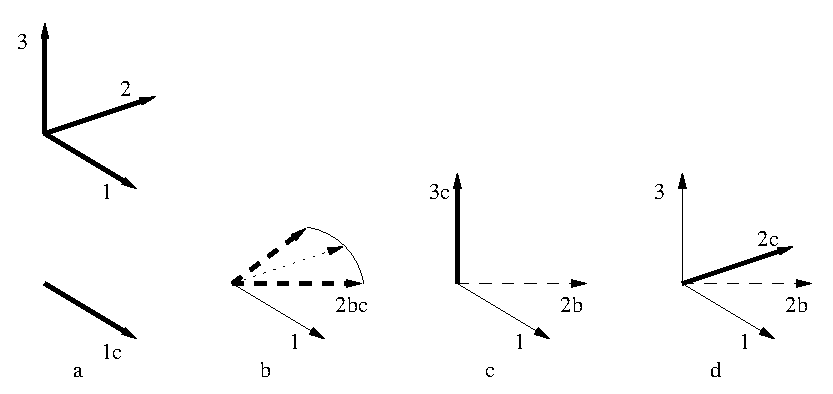
\includegraphics[width=.9\textwidth]{MatR2vec}
\caption{Construction of $3 \times 3$ orientation matrix from two
non-parallel vectors.}
\label{fig:general:orientation-matrices:MatR2vec}
\end{figure}

\subsection{($3 \times 3$) Orientation Matrix}
\label{sec:OrientationMatrix}
Implements the type \ty{OrientationMatrix}.
\begin{enumerate}
\item general case: two vectors that define an orthonormal reference
system, each of them preceded by its index in the final orientation matrix.
The procedure that builds the orientation matrix from the two vectors
is illustrated in Figure~\ref{fig:general:orientation-matrices:MatR2vec}.
The first vector, vector 1 in subfigure (a), is normalized and assumed
to represent the desired direction.
The second vector, vector 2' in subfigure (b), simply concurs
in the definition of the plane the vector that is not given is normal to.
The third vector, vector 3 in subfigure (c), results from the cross-product
of the first two vectors, after normalization.
The actual direction of the second vector, vector 2 in subfigure (d),
results from the cross product of the third and the first vector.
Examples:
\begin{verbatim}
    1, 1.,0.,0., 2, 0.,1.,0.
    1, (real ALPHA = pi/6.; cos(ALPHA)), sin(ALPHA), 0.,
        3, 0.,0.,1.
\end{verbatim}
The first example represents the identity matrix, i.e.\ no rotation 
occurs with respect to the global reference frame: direction 1
in the local frame is parallel to \texttt{1.,0.,0.}, which represents
direction 1 in the global frame, while direction 2 in the local frame
is parallel to \texttt{0.,1.,0.}, which represents direction 2
in the global frame.

The second example describes a rotation of $ \pi/6 $ radian about
global direction 3: direction 1 in the local frame results from 
composing \kw{cos}\texttt{(pi/6.)} in global direction 1
and \kw{sin}\texttt{(pi/6.)}
in global direction 2, while direction 3 in the local frame remains
parallel to \texttt{0.,0.,1.}, which represents direction 3 in the global
frame.

\item a variant of the above, which may be useful when only one
direction really matters, is illustrated in the example below:
\begin{verbatim}
    1, 1.,0.,0., 2, guess
\end{verbatim}
The keyword \kw{guess} tells the parser to generate a random vector
that is orthogonal to the given one, which is used as the direction
indicated by the index (2 in the example).
The vector is computed based on a very simple algorithm: it contains
\begin{itemize}
        \item 1.0 corresponding to the index with smallest module,
        $v_1\plbr{\mathrm{min}}$;
	\item $-v_1\plbr{\mathrm{min}}/v_1\plbr{\mathrm{max}}$
	corresponding to the index with the largest module,
	$v_1\plbr{\mathrm{max}}$;
	\item 0.0 on the remaining index.
\end{itemize}

\item identity matrix: keyword \kw{eye}; the identity matrix,
which means there is no rotation with respect to the global reference
frame.

\item a complete orientation matrix: keyword \kw{matr}
followed by the nine, row-oriented, coefficients, namely
$ r_{11} $, $ r_{12} $, \ldots, $ r_{33} $.
\emph{Note: no orthogonality check is performed; be sure an orthogonal
matrix, within the desired tolerance, is input}.

\item Euler angles: keyword \kw{euler}, followed by the three
values, as output by structural nodes.
The keywords \kw{euler123}, \kw{euler313} and \kw{euler321}
allow to use orientations in the sequence specified by the keyword.
\begin{Verbatim}[commandchars=\\\{\}]
    \{ \kw{euler} | \kw{euler123} | \kw{euler313} | \kw{euler321} \} ,
        [ \kw{degrees} , ]
        \bnt{angle_1} , \bnt{angle_2} , \bnt{angle_3}
\end{Verbatim}
\fbox{\begin{minipage}{.93\textwidth}%
Note: the output in the \texttt{.mov} file is in degrees,
while in input MBDyn requires angles in radians,
unless the values are preceded by the keyword \kw{degrees}.
\end{minipage}}

\emph{Note: the definition of the three angles that are used 
by the code to express orientations may vary between versions.
Currently, Bryant-Cardano angles are used in place of Euler
angles; see the note related to the output of the structural nodes
in Section~\ref{sec:NODE:STRUCTURAL:OUTPUT}, and the Technical Manual.
The code will remain consistent, i.e. the same angle
definition will be used for input and output, but models
over versions may become incompatible, so this syntax should 
really be used only as a means to quickly reproduce in the input
an orientation as resulting from a previous analysis.}

\item Orientation vector: keyword \kw{vector}, followed by the three
values, as output by structural nodes.
The resulting matrix is computed as
\begin{equation}
	\T{R} = \exp\plbr{\T{v}\times{}}
\end{equation}
\end{enumerate}

\subsection{$6 \times 6$ Matrix}
\label{sec:Mat6x6}
Implements the type \ty{Mat6x6}.
\begin{enumerate}
    \item general case: a sequence of 36 reals, comma-separated, that
    represent the row-oriented coefficients $ a_{11} $, $ a_{12}$ ,
    \ldots, $ a_{65} $, $ a_{66} $.
    \item ANBA format: keyword \kw{anba}, followed by 36 reals, 
    comma-separated, that represent the coefficients of the beam stiffness
    matrix as generated by the beam section analysis code ANBA,
    namely the following transformation is performed:
    \begin{itemize}
        \item axis $ x $, in the section plane in ANBA notation, 
	becomes axis 2 in MBDyn notation;    
	\item axis $ y $, in the section plane in ANBA notation, 
	becomes axis 3 in MBDyn notation;    
	\item axis $ z $, the beam axis in ANBA notation, 
	becomes axis 1 in MBDyn notation;    
    \end{itemize}
    \emph{Note: this format is mainly intended for backwards compatibility
    with older versions of that beam section analysis software,
    which used a different numbering convention for the reference frame
    that is local to the beam section.}
    \item symmetric matrix: keyword \kw{sym}, followed by a sequence
    of 21 reals, comma-separated, that represents the upper triangle,
    row-oriented coefficients of a symmetric matrix, 
    e.g. $ a_{11} $, \ldots , $ a_{16} $, $ a_{22} $,
    \ldots , $ a_{26} $, \ldots, $ a_{66} $.
    \item diagonal matrix: keyword \kw{diag}, followed by a sequence
    of 6 reals, comma-separated, that represent the diagonal coefficients 
    of a diagonal matrix.
    \item identity matrix: keyword \kw{eye}; the matrix is initialized
    as the identity matrix, that is a null matrix except for the diagonal 
    coefficients that are 1.
    \item null matrix: keyword \kw{null}; the matrix is initialized 
    with zeros.
\end{enumerate}
\subsection{$6 \times N$ Matrix}
\label{sec:Mat6xN}
Implements the type \ty{Mat6xN}.
\begin{enumerate}
    \item general case: a sequence of $6 \times N$ reals, comma-separated, that
    represent the row-oriented coefficients $ a_{11} $, $ a_{12}$ ,
    \ldots, $ a_{6\plbr{N-1}} $, $ a_{6N} $.
    \item ANBA format: keyword \kw{anba}, followed by $6 \times N$ reals,
    comma-separated, that represent the coefficients of the beam stiffness
    matrix as generated by the code ANBA, namely the following
    transformation is performed:
    \begin{itemize}
        \item axis $ x $, in the section plane in ANBA notation, 
	becomes axis 2 in MBDyn notation;    
	\item axis $ y $, in the section plane in ANBA notation, 
	becomes axis 3 in MBDyn notation;    
	\item axis $ z $, the beam axis in ANBA notation, 
	becomes axis 1 in MBDyn notation;    
    \end{itemize}
    \item null matrix: keyword \kw{null}; the matrix is initialized 
    with zeros.
\end{enumerate}


\section{Input Related Cards} 
(Almost) everywhere in the input file the statement cards defined 
in the following can be used.
They are handled directly by the parsing object, and merely act as
an indirect reference to entities that are not explicitly enumerated.
They are:



\subsection{Constitutive Law}\label{sec:CONSTITUTIVE-LAW}
%\begin{verbatim}
\begin{Verbatim}[commandchars=\\\{\}]
    \bnt{card} ::= \kw{constitutive law} : \bnt{label} ,
        [ \kw{name} , " \bnt{name} " , ]
        \bnt{dim} , (\htmlref{\ty{ConstitutiveLaw}\be{\bnt{dim}\kw{D}}}{sec:ConstitutiveLaw}) \bnt{constitutive_law} ;
\end{Verbatim}
%\end{verbatim}
Constitutive laws are grouped by their dimensionality \nt{dim},
which (up to now) can be any of 1, 3 and 6.
The \nt{constitutive\_law} is parsed according to the rules
described in Section~\ref{sec:ConstitutiveLaw},
and can be referenced later when it needs to be used.



\subsection{C81 Data}\label{sec:C81-DATA}
This keyword allows to define and read the \kw{c81 data} 
airfoil tables that are used by aerodynamic elements.
%\begin{verbatim}
\begin{Verbatim}[commandchars=\\\{\}]
    \bnt{card} ::= \kw{c81 data} : \bnt{label} [ , \kw{name} , " \bnt{name} " ]
        " \bnt{filename} "
        [ , \kw{tolerance} , \bnt{tolerance} ]
        [ , \{ \kw{free format} | \kw{nrel} | \kw{fc511} \} ]
        [ , \kw{flip} ]
        [ , \kw{echo} , " \bnt{output_filename} " [ , \kw{free format} ] ] ;
\end{Verbatim}
%\end{verbatim}
Data is read from file \nt{filename} according to the format specified
in the following.

The optional keyword \kw{tolerance} allows to specify the tolerance
that is used to determine the boundaries of the linear portion
of the lift curve slope.

The traditional format is used unless a format is specified using any
of the keywords \kw{free format}, \kw{nrel} or \kw{fc511}
(the latter is intentionally not documented).
The format is automatically inferred by reading the heading line
of the input file.

The optional keyword \kw{flip} instructs MBDyn to ``flip'' the data,
i.e.\ treat the airfoil data as if the sign of the angle of attack
changed along with that of the lift and moment coefficients,
but not that of the drag coefficient.
This corresponds to considering the airfoil ``upside down''.

The optional keyword \kw{echo} allows to specify the name of the file
that will be generated with the data just read, for cross-checking purposes.
If the following optional keyword is \kw{free format}, or if data was read
in free format, the echo will also be in free format.
Otherwise, it will be in the traditional format.

\subsubsection{Traditional Format}
The file is in textual form; the traditional format (the default) is:
\begin{itemize}
\item first line: \texttt{"\%30s\%2d\%2d\%2d\%2d\%2d\%2d"} 
where the first 30 chars are a title string, currently ignored by MBDyn,
followed by 6 consecutive two-digit integers that indicate:
	\begin{itemize}
	\item the number \texttt{ML} of \emph{Mach} points for $C_l$;
	\item the number \texttt{NL} of angle of attack points for $C_l$;
	\item the number \texttt{MD} of \emph{Mach} points for $C_d$;
	\item the number \texttt{ND} of angle of attack points for $C_d$;
	\item the number \texttt{MM} of \emph{Mach} points for $C_m$;
	\item the number \texttt{NM} of angle of attack points for $C_m$.
	\end{itemize}
The example in \texttt{var/naca0012.c81} contains:
{\small
\begin{verbatim}
1........01........01........0MLNLMDNDMMNM; not part of format
PROFILO NACA 0012             11391165 947
\end{verbatim}
}
\item the format of each following line is up to 10 fields of 7 chars each;
records longer than 10 fields are broken on multiple lines,
with the first field filled with blanks;
\item a block containing the $C_l$ data, made of:
	\begin{itemize}
	\item a record with the first field blank, followed by
	the \texttt{ML} \emph{Mach} values for the $C_l$;
	\item \texttt{NL} records containing the angle of attack
	in the first field, followed by \texttt{ML} values of $C_l$
	for each \emph{Mach} number; angles of attack wrap around 
	360 deg, starting from -180 deg.
	\end{itemize}
The example provided in file \texttt{var/naca0012.c81}
contains 11 \emph{Mach} points and 39 angle of attack records for the $C_l$
of the NACA0012 airfoil at high (unspecified) \emph{Reynolds}:
{\small
\begin{verbatim}
......7......7......7......7......7......7......7......7......7......7; not part of format
       0.     .20    .30    .40    .50    .60    .70    .75    .80
       .90    1.
-180.  0.     0.     0.     0.     0.     0.     0.     0.     0.
       0.     0.
-172.5 .78    .78    .78    .78    .78    .78    .78    .78    .78
       .78    .78
...
\end{verbatim}
}
\item a block containing the $C_d$ data, same as for $C_l$,
with \texttt{MD} \emph{Mach} points and \texttt{ND} angle of attack records;
\item a block containing the $C_m$ data, same as for $C_l$,
with \texttt{MM} \emph{Mach} points and \texttt{NM} angle of attack records.
\end{itemize}

\subsubsection{Free Format}
Finally, to allow higher precision whenever available, a native format,
based on \texttt{c81}, called \kw{free format}, is available.
It basically consists in the \texttt{c81} format without continuation lines
and with arbitrary precision, with fields separated by blanks.
The header is made of an arbitrary string, terminated by a semicolon `\texttt{;}',
followed by the six numbers that define the dimensionality of the expected data.

\paragraph{Example.} \
\begin{verbatim}
# FREE FORMAT
this is the header; 2 8 2 2 2 2
        0.0   0.9
-180.0  0.0   0.0
-170.0  1.0   0.9
 -90.0  0.0   0.0
 -10.0 -1.0  -0.9
  10.0  1.0   0.9
  90.0  0.0   0.0
 170.0 -1.0  -0.9
 180.0  0.0   0.0
        0.0   0.9
-180.0  0.1   0.1
 180.0  0.1   0.1
        0.0   0.9
-180.0  0.0   0.0
 180.0  0.0   0.0
\end{verbatim}

\subsubsection{NREL}
The \kw{nrel} format is used to provide airfoil data for wind turbines.
The format is very compact, but does not allow to account for Mach
dependence, and requires the same angle of attack resolution
for all three coefficients.
See AeroDyn's User Guide \cite{AERODYN-UG-2002} for a description
of the format.
Please note that MBDyn only supports one airfoil per file,
and only considers static coefficients from line 15 on.

\emph{To be completed.}

\subsubsection{Alternative Format}
An alternative format, required by some projects, can be used by supplying
the optional switch \kw{fc511}; it is intentionally not documented.

\subsubsection{Format Conversion}

Traditional format files can be automatically converted in free format
using the \texttt{c81test(1)} utility:
\begin{verbatim}
    $ c81test -d var/naca0012_free_format.c81 var/naca0012.c81
\end{verbatim}
generates a free format version of the NACA 0012 airfoil data
provided in the distribution.

\subsubsection{Miscellaneous}
A simple program that allows to read and plot the C81 tables
is available at \\
\htmladdnormallink{\texttt{http://homepage.mac.com/jhuwaldt/java/Applications/TableReader/TableReader.html}}
        {http://homepage.mac.com/jhuwaldt/java/Applications/TableReader/TableReader.html} \\
(thanks to Marco Fossati for pointing it out).

A simple utility that parses the C81 file and computes 
the aerodynamic coefficients for a given pair of angle of attack 
and Mach number is \texttt{c81test(1)}, available in the MBDyn utils suite.
This routine uses exactly the same code internally used by MBDyn,
so it should be considered a check of the code rather than a real tool.


\subsection{Drive Caller}\label{sec:DRIVE-CALLER}
The \kw{drive caller} directive
%\begin{verbatim}
\begin{Verbatim}[commandchars=\\\{\}]
    \bnt{card} ::= \kw{drive caller} : \bnt{label} ,
        [ \kw{name} , " \bnt{name} " , ]
        (\htmlref{\ty{DriveCaller}}{sec:DriveCaller}) \bnt{drive_caller} ;
\end{Verbatim}
%\end{verbatim}
allows to define
a \hyperref{\kw{drive caller}}{\kw{drive caller} (see Section~}{)}{sec:DriveCaller}
that can be subsequently reused.
It is useful essentially in two cases:
\begin{enumerate}
	\renewcommand{\labelenumi}{\alph{enumi})}
	\item to define a \htmlref{\kw{drive}}{sec:DriveCaller}
	that will be used many times throughout a model;
	\item to define a \htmlref{\kw{drive}}{sec:DriveCaller} 
	that needs to be used in a later defined part of a model, 
	in order to make it parametric.
\end{enumerate}



\subsection{Hydraulic fluid}\label{sec:HYDRAULIC-FLUID}
The \kw{hydraulic fluid} directive:
%\begin{verbatim}
\begin{Verbatim}[commandchars=\\\{\}]
    \bnt{card} ::= \kw{hydraulic fluid} : \bnt{label} , 
        \bnt{fluid_type} , \bnt{fluid_properties} ;
\end{Verbatim}
%\end{verbatim}
allows to define a hydraulic fluid to be later used in hydraulic elements,
see Section~\ref{sec:EL:HYDR}.
The fluid is identified by the \nt{label}. 
The \nt{fluid\_type}s, with the related \nt{fluid\_properties}, are
described in \ref{sec:HydraulicFluid}



\subsection{Include}\label{sec:INCLUDE}
The \kw{include} directive
%\begin{verbatim}
\begin{Verbatim}[commandchars=\\\{\}]
    \bnt{card} ::= \kw{include} : " \bnt{file_name} " ;
\end{Verbatim}
%\end{verbatim}
allows to include the contents of the file
\nt{file\_name},
which must be a valid filename for the operating system in
use.
The file name must be enclosed in double quotes (\texttt{"}).
The full (absolute or relative) path must be given if the included file 
is not in the directory of the including one.

\bigskip

\fbox{There is no check for recursive \kw{include} directives, so 
{\bf the user must take care of recursion}.}

\bigskip

The \kw{include} directive forces the parser to scan the included file
\nt{file\_name} before continuing with the including one.
This is very useful if, for instance, a big model can be made of many
small models that are meaningful by themselves.

It can be used to replicate parts of the model, by simply using parametric 
labels for nodes, elements, reference systems, and setting a bias value 
before multiple-including the same bulk data file.
Examples of this usage are given in the tutorials
\htmladdnormallink{(\texttt{http://www.aero.polimi.it/mbdyn/documentation/tutorials/})}
	{http://www.aero.polimi.it/mbdyn/documentation/tutorials/}.



\subsection{Module Load}
\label{sec:GENERAL:MODULE-LOAD}
The \kw{module load} directive:
%\begin{verbatim}
\begin{Verbatim}[commandchars=\\\{\}]
    \bnt{card} ::= \kw{module load} : " \bnt{file_name} "
        [ , \bnt{module_arglist} ] ;

    \bnt{module_arglist} ::= \bnt{arg} [ , ... ]
\end{Verbatim}
%\end{verbatim}
where \nt{file\_name} is the name of a runtime loadable object,
causes the object to be opened, and a function \texttt{module\_init()},
with prototype
%\begin{verbatim}
\begin{Verbatim}[commandchars=\\\{\}]
        \textcolor{green}{extern} \textcolor{red}{"C"} \textcolor{green}{int}
        module_init(\textcolor{green}{const char} *module_name,
                \textcolor{green}{void} *data_manager, \textcolor{green}{void} *mbdyn_parser);
\end{Verbatim}
%\end{verbatim}
to be executed.

The function is assumed to perform the operations required to initialize
the module, eventually taking advantage of the parsing
and of the data manager; see the technical manual for details.

The function is also expected to take care of the optional \nt{module\_arglist}
arguments; in detail, module developers are encouraged to support
\kw{help} as the first optional argument.
The presence of this argument should result in printing to standard output
as much information as possible about the use of the module.

The typical use consists in registering some methods for later use.
A clear example is given in
\begin{verbatim}
        modules/module-wheel2/module-wheel2.cc
\end{verbatim}
where the \texttt{module\_init()} function registers
the \kw{user defined} element called \kw{wheel2}
in the set of user-defined element handlers.
The module can be retrieved later using the syntax described
in Section~\ref{sec:EL:BASE:USER_DEFINED}.
Note, however, that the \texttt{module\_init()} function may be used
for any purpose.
A typical use consists in registering any kind of handlers
for subsequent use.

Run-time module loading is taken care of by GNU's \texttt{libltdl}.
Modules are compiled using \texttt{libtool} for portability purposes.
The resulting modules take the name
\texttt{libmodule-<name>.la}.

Modules are installed by default in the directory
\texttt{\$\{prefix\}/libexec}.
When loaded using only the module name, the default directory is searched.
The run-time loading path can be modified by the 
\kw{loadable path} statement described
in Section~\ref{sec:CONTROLDATA:LOADABLE_PATH}.

Although \texttt{libltdl} is supposed to be portable on a wide variety
of platforms (this is what it is designed for, all in all),
run-time loading within MBDyn is mainly tested using Linux.
Users are encouraged to report problems they might encounter,
especially when building modules for different platforms,
as this would help making MBDyn more portable.



\subsection{Print symbol table}
The \kw{print symbol table} directive:
%\begin{verbatim}
\begin{Verbatim}[commandchars=\\\{\}]
    \bnt{card} ::= \kw{print symbol table} [ : { \kw{all} | \bnt{namespace_list} } ] ;

    \bnt{namespace_list} ::= \bnt{namespace} [ , \bnt{namespace_list} ]
\end{Verbatim}
%\end{verbatim}
allows to print to standard output the contents of the parser's symbol
table at any stage of the input phase.
This may be useful for model debugging purposes.

When no arguments are provided, it prints the symbol table of the math parser.
Otherwise, it prints the symbol table associated with a specific namespace,
according to the list of arguments (all namespaces when the keyword \kw{all} is used).



\subsection{Reference}
The \kw{reference} directive:
%\begin{verbatim}
\begin{Verbatim}[commandchars=\\\{\}]
    \bnt{card} ::= \kw{reference} : \bnt{unique_label} , 
        [ \kw{name} , (\ty{string}) \bnt{name} , ]
        (\htmlref{\ty{Vec3}}{sec:Vec3}) \bnt{absolute_position} ,
        (\htmlref{\ty{OrientationMatrix}}{sec:OrientationMatrix}) \bnt{absolute_orientation_matrix} ,
        (\htmlref{\ty{Vec3}}{sec:Vec3}) \bnt{absolute_velocity} ,
        (\htmlref{\ty{Vec3}}{sec:Vec3}) \bnt{absolute_angular_velocity} ;
\end{Verbatim}
%\end{verbatim}
A \kw{reference} system is declared and defined.
It must be given a unique identifier, scanned by the math parser
(which means that any regular expression is allowed, and the result is
rounded up to the nearest unsigned integer).
The entries \nt{absolute\_*} are parsed by routines that
compute absolute (i.e.\ referring to the global frame) entities
starting from a given entity in a given reference frame.
These routines are very general, and make intense use of the 
\kw{reference} entries themselves, which means that a reference 
can be recursively defined by means of previously defined 
\kw{reference} entries.

\bigskip

Alternative form, based on Denavit-Hartenberg parameters,
which are particularly used in robotics.
It defines the reference system of the second part of a joint with respect to the first part,
when the two parts are connected by revolute joints.
%\begin{verbatim}
\begin{Verbatim}[commandchars=\\\{\}]
    \bnt{card} ::= \kw{reference} : \bnt{unique_label} , 
        [ \kw{name} , " \bnt{name} " , ]
        \kw{Denavit Hartenberg} ,
        [ \kw{reference} , \{ \kw{global} | \bnt{ref_label} \} , ]
        \bnt{d} , \bnt{theta} , \bnt{a} , \bnt{alpha} ;
\end{Verbatim}
%\end{verbatim}
where:
\begin{itemize}
\item \nt{d}: offset $d$ along previous $z$ axis to the common normal (the current $x$ axis);

\item \nt{theta}: the angle $\theta$ about previous $z$ from previous to current $x$ axis;

\item \nt{a}: length $a$ of the common normal; for revolute joints, the radius of the previous $z$;

\item \nt{alpha}: the angle $\alpha$ about the common normal, from previous to new $z$ axis.
\end{itemize}
The configuration of the first part of the joint is identified by an axis $z_1$ and a point $\text{P}_1$ on it.
The configuration of the second part of the joint is identified by an axis $z_2$;
point $\text{P}_2$ on the second part of the joint results from the definition itself,
and is not strictly relevant for the definition.
If the two axes are not parallel, they have a common normal, $x_2$, that crosses both;
otherwise, one can arbitrarily choose $x_2$ as a direction orthogonal to both $z_1$
(and $z_2$, since they are parallel, or even coincident).
Choose $x_1$ as a vector normal to $z_1$, originating from the reference point of the first part of the joint, $\text{P}_1$,
and directed towards the reference point of the second part of the joint, $\text{P}_2$
(this is not strictly required, as one can choose axis $x_1$ at will, as it only provides the reference for the joint rotation).
In general, $x_1$ will not be able to intersect axis $z_2$, unless axes $z_1$ and $z_2$ are co-planar.
Point $\text{P}_2$ is the intersection between axes $x_2$ and $z_2$.
If needed, axes $y_1$ and $y_2$ are defined according to the right-hand rule.
Then:
\begin{itemize}
\item \nt{d} is the distance, along $z_1$, between the reference point of the first part, $\text{P}_1$, and the plane determined by axes $z_2$ and $x_2$;

\item \nt{theta} is the angle about axis $z_1$ between axes $x_2$ and $x_1$; it represents the actual rotation of the joint;

\item \nt{a} is the distance between axes $z_1$ and $z_2$, which is along axis $x_2$;

\item \nt{alpha} is the angle formed by axis $z_2$ with respect to axis $z_1$; it corresponds to a rotation about axis $x_2$.
\end{itemize}

The new reference data are
\begin{subequations}
\begin{align}
	\T{x}_\text{new}
	&=
	\T{x}_\text{old}
	+
	\TT{R}_\text{old} \plbr{
		\nt{d} \, \T{e}_3
		+
		\text{exp}\plbr{\plbr{\nt{theta} \, \T{e}_3} \times{}} \cdot \plbr{\nt{a} \, \T{e}_1}
	}
	\\
	\TT{R}_\text{new}
	&=
	\TT{R}_\text{old} \text{exp}\plbr{\plbr{\nt{theta} \, \T{e}_3} \times{}} \text{exp}\plbr{\plbr{\nt{alpha} \, \T{e}_1} \times{}}
	\\
	\T{v}_\text{new}
	&=
	\T{v}_\text{old}
	+
	\T{\omega}_\text{old} \times \TT{R}_\text{old} \plbr{
		\nt{d} \, \T{e}_3
		+
		\text{exp}\plbr{\plbr{\nt{theta} \, \T{e}_3} \times{}} \cdot \plbr{\nt{a} \, \T{e}_1}
	}
	\\
	\T{\omega}_\text{new}
	&=
	\T{\omega}_\text{old}
\end{align}
\end{subequations}
where the subscript ``old'' refers to the reference frame with label \nt{ref\_label1}, if any, or otherwise to the global reference system.

\subsubsection{Use of Reference Frames}
Every time an absolute or a relative geometric or physical entity is
required, it is processed by a set of routines that allow the entity to be
expressed in the desired reference frame.
The following cases are considered:
\begin{itemize}
    \item relative position (physical)
    \item absolute position (physical)
    \item relative orientation matrix (physical)
    \item absolute orientation matrix (physical)
    \item relative velocity (physical)
    \item absolute velocity (physical)
    \item relative angular velocity (physical)
    \item absolute angular velocity (physical)
    \item relative arbitrary vector (geometric)
    \item absolute arbitrary vector (geometric)    
\end{itemize}
The caller is responsible for the final interpretation of the input. 
The caller always supplies the routines a default reference structure
the input must be referred to.
So, depending on the caller, the entry can be in the following forms:
\begin{enumerate}
\item \bnt{entity}: \\ 
	the data supplied in \nt{entity} is intended 
	in the default reference frame
\item \texttt{\kw{reference} , \bnt{reference\_type} , \bnt{entity}}: \\
	the data are in \nt{reference\_type} reference frame, where
%\begin{verbatim}
\begin{Verbatim}[commandchars=\\\{\}]
        \bnt{reference_type} ::= \{ \kw{global} | \kw{node} | \kw{local} \}
\end{Verbatim}
%\end{verbatim}
\item \texttt{\kw{reference} , \bnt{reference\_label} , \bnt{entity}}: \\
	the data are in \nt{reference\_label} reference frame. 
	This reference frame must be already defined. 
\end{enumerate}
In some cases, significantly in case of joints that connect two nodes
$a$ and $b$, special reference types are allowed
when reading specific entities related to the second node.
These reference types compute the value of the entity with respect
to the reference frame associated to the first node, $a$:
\begin{enumerate}
\item \kw{other position}: \\
	a relative position $\tilde{\T{p}}$ is intended in the other node's
	reference frame, with respect to the relative position $\tilde{\T{f}}_a$
	already specified for the other node,
\begin{equation}
	\tilde{\T{f}}_b = \TT{R}_b^T\plbr{
		\T{x}_a + \TT{R}_a \plbr{
			\tilde{\T{f}}_a
			+ \tilde{\T{p}}
		}
		- \T{x}_b
	} ,
\end{equation}
	which is the solution of equation
\begin{equation}
	\T{x}_a + \TT{R}_a \plbr{\tilde{\T{f}}_a + \tilde{\T{p}}}
	= \T{x}_b + \TT{R}_b \tilde{\T{f}}_b ;
\end{equation}

\item \kw{other orientation}: \\
	a relative orientation $\tilde{\TT{R}} $ is intended in the other node's
	reference frame, with respect to the relative orientation
	$\tilde{\TT{R}}_{ha}$ already specified for the other node,
\begin{equation}
	\tilde{\TT{R}}_{hb} = \TT{R}_b^T \TT{R}_a \tilde{\TT{R}}_{ha} \tilde{\TT{R}} ,
\end{equation}
	which is the solution of equation
\begin{equation}
	\TT{R}_a \tilde{\TT{R}}_{ha} \tilde{\TT{R}}
	= \TT{R}_b \tilde{\TT{R}}_{hb} ;
\end{equation}

\item \kw{other node}: \\
	a relative position $\tilde{\T{p}}$
	or a relative orientation $\tilde{\TT{R}}$
	are intended in the other node's reference frame,
\begin{subequations}
\begin{align}
	\tilde{\T{f}}_b &= \TT{R}_b^T\plbr{
		\T{x}_a + \TT{R}_a \tilde{\T{p}}
		- \T{x}_b
	} \\
	\tilde{\TT{R}}_{hb} &= \TT{R}_b^T \TT{R}_a \tilde{\TT{R}} ,
\end{align}
\end{subequations}
	which are the solutions of equations
\begin{subequations}
\begin{align}
	\T{x}_a + \TT{R}_a \tilde{\T{p}}
	&= \T{x}_b + \TT{R}_b \tilde{\T{f}}_b \\
	\TT{R}_a \tilde{\TT{R}}
	&= \TT{R}_b \tilde{\TT{R}}_{hb} .
\end{align}
\end{subequations}
\end{enumerate}

\paragraph{Example.} \
\begin{itemize}
    \item absolute position:
    \begin{verbatim}
    null
    reference, global, null
    reference, 8, 1., sin(.3*pi), log(3.)
    \end{verbatim}
    \item relative orientation matrix (e.g.\ as required by many constraints and
    thus referred to a node):
    \begin{verbatim}
    eye
    reference, node, eye
    reference, 8,
        3, 0., 1., 0., 
        1, .5, sqrt(3)/2., 0.
    \end{verbatim}
\end{itemize}
Notes: 
\begin{itemize}
    \item the global reference frame has position $ \cubr{0, 0, 0} $,
    orientation matrix \kw{eye}, velocity $ \cubr{0, 0, 0} $ and angular
    velocity $ \cubr{0, 0, 0} $.
    \item if the caller is not related to a node, the reference type
    \kw{node} should not be defined. 
    In this case it is considered equivalent to \kw{local}.
    \item when processing a velocity or an angular velocity, the resulting
    value always accounts for the velocity and angular velocity of the frame
    the entry is referred to. 

    As an example, if a node is defined in a reference frame $\T{R}_R$
    that has non-null angular velocity $ \T{\Omega}_R $, and the position 
    $ \T{x}_{\text{input}} $ of the node is not coincident
    with the origin $ \T{X}_R $ of the reference frame
    it is attached to, its global velocity and angular velocity result
    as the composition of the input values and of those of the reference 
    frame:
    \begin{eqnarray*}    
        \T{w} & = & \T{R}_R \T{\omega}_{\text{input}} + \T{\Omega}_R \\
	\T{v} & = & \T{R}_R \T{v}_{\text{input}} + \T{V}_R
		+\T{\Omega}_R\times\plbr{\T{R}_R \T{x}_{\text{input}}}
    \end{eqnarray*}
    This, for instance, eases the input of all the parts of a complex system
    that is moving as a rigid body, by defining a reference frame with the
    proper initial velocities, and then referring all the entities, e.g.\ the 
    nodes, to that frame, with null local velocity.
\end{itemize}  
{\em
    Recalling the declaration and the definition of reference frames,
    a simple reference frame definition, with all the entries referring 
    by default to the global system, would be:
    \begin{verbatim}
    reference: 1000,
        null,
        eye,
        null,
        null;
    \end{verbatim}
    which represents a redefinition of the global system.
    A more verbose, and self-explanatory definition would be:
    \begin{verbatim}
    reference: 1000,
        reference, global, null,
        reference, global, eye,
        reference, global, null,
        reference, global, null;			 
    \end{verbatim}
    the reference frame one is referring to must be repeated for all the entries
    since they must be allowed to refer to whatever frame is preferred 
    by the user.
    A fancier definition would be:
    \begin{verbatim}
    reference: Rotating_structure, 
        reference, Fixed_structure, null,
        reference, Spindle_1,
            1, 0.,0.,1., 
            3, 0.,1.,0.,
        reference, Fixed_structure, null,
        reference, Spindle_1, 0.,0.,Omega_1;
    \end{verbatim}
}

\subsubsection{Output}
The reference frames are used only during the input phase, 
where they help referring entities either absolute 
or relative to other entities depending on their internal representation
during the analysis.
As such, reference frames cannot be ``used'' or ``visualized'' neither 
directly nor indirectly at any time during the analysis or by interpreting
the output, because they do not ``evolve'' nor are attached
to any state-dependent entity.
To allow their debugging, however, they can be output in the global
reference frame according to the representation of structural nodes,
as described in Section~\ref{sec:NODE:STRUCTURAL:OUTPUT}, 
by using the \kw{default output} directive 
with the value \kw{reference frames}, as detailed
in Section~\ref{sec:CONTROLDATA:DEFAULTOUTPUT}.



\subsection{Remark}
The \kw{remark} directive:
%\begin{verbatim}
\begin{Verbatim}[commandchars=\\\{\}]
    \bnt{card} ::= \kw{remark} [ : \bnt{math_expression} [ , ... ] ] ;
\end{Verbatim}
%\end{verbatim}
This directive simply prints to stdout the (list of) expression(s) \nt{math\_expression}.
It is used to allow rough input debugging. The file name and line number
are logged first, followed by the result of the evaluation of the expression(s list). 

\paragraph{Example.} \
A file ``remarks'', containing only the statements
\begin{verbatim}
    remark: "square root of 2", sqrt(2);
    set: (
        real EA = 1e6; # N, axial stiffness
        real GA = 1e6; # N, shear stiffness
        real EJ = 1e3; # Nm^2, bending stiffness
        real GJ = 1e3; # Nm^2, torsional stiffness
    0);
    remark: "Stiffness properties", EA, GA, EJ, GJ;
\end{verbatim}
results in
\begin{verbatim}
user@host:~>$ mbdyn -f remarks

MBDyn - Multi-Body Dynamics 1.6.2
configured on Jun 26 2015 at 10:17:02

Copyright 1996-2015 (C) Paolo Mantegazza and Pierangelo Masarati,
Dipartimento di Ingegneria Aerospaziale <http://www.aero.polimi.it/>
Politecnico di Milano                   <http://www.polimi.it/>

MBDyn is free software, covered by the GNU General Public License,
and you are welcome to change it and/or distribute copies of it
under certain conditions.  Use 'mbdyn --license' to see the conditions.
There is absolutely no warranty for MBDyn.  Use "mbdyn --warranty"
for details.

reading from file "remarks"
line 1, file <remarks>: square root of 2, 1.41421
line 8, file <remarks>: Stiffness properties, 1e+06, 1e+06, 1000, 1000
MBDyn terminated normally
user@host:~>$
\end{verbatim}
Notice that in the example above the first expression is actually a string,
as it was required up to version 1.6.1; this is no longer required.

\subsection{Set}
The \kw{set} directive:
%\begin{verbatim}
\begin{Verbatim}[commandchars=\\\{\}]
    \bnt{card} ::= \kw{set} : \bnt{math_expression} ;
\end{Verbatim}
%\end{verbatim}
This directive simply invokes the math parser to evaluate the expression
\nt{math\_expression} and then discards the result.

It can be used to declare new variables, or to set the values
of existing ones.
This feature is very useful, since it allows to build parametric models,
and to reuse generic model components.

\paragraph{Example.} \
\begin{verbatim}
    set: integer LABEL = 1000;    # a label
    set: real E = 210e+9;         # Pa, steel's elastic module
    set: real A = 1e-4;           # m^2, a beam's cross section
    set: real K = E*A;            # N, a beam's axial stiffness
\end{verbatim}



\subsection{Setenv}
The \kw{setenv} directive:
%\begin{verbatim}
\begin{Verbatim}[commandchars=\\\{\}]
    \bnt{card} ::= \kw{setenv} :
        [ \kw{overwrite} , \{ \kw{yes} | \kw{no} | (\ty{bool}) \bnt{overwrite} \} , ]
        " \bnt{varname} [ = \bnt{value} ] " ;
\end{Verbatim}
%\end{verbatim}
This directive sets the environment variable \nt{varname} 
to \nt{value}, if given; otherwise, the variable
is unset.
If \kw{overwrite} is set, the variable is overwritten, 
if already set.
By default, \kw{overwrite} is set according to \texttt{setenv(3)}'s
overwrite parameter (\kw{no}).
\begin{verbatim}
    # set FILE to "test", if it does not exist
    setenv: "FILE=test";
    # set FILE to "test", even if it exists
    setenv: overwrite, yes, "FILE=test";
    # unset FILE
    setenv: "FILE";
    # set FILE to the empty string, if it does not exist
    setenv: "FILE=";
\end{verbatim}
See \texttt{setenv(3)} and \texttt{unsetenv(3)}
(or \texttt{putenv(3)}, if the former is not available)
man pages for details.




\subsection{Template Drive Caller}\label{sec:TPL-DRIVE-CALLER}
The \kw{template drive caller} directive
%\begin{verbatim}
\begin{Verbatim}[commandchars=\\\{\}]
    \bnt{card} ::= \kw{template drive caller} : \bnt{label} , \{ " \bnt{dim_name} " | (\ty{integer}) \bnt{dim} \} ,
        (\htmlref{\ty{TplDriveCaller}\be{\bnt{Entity}}}{sec:TplDriveCaller}) \bnt{tpl_drive_caller} ;

    \bnt{dim_name} ::= \{ \kw{1} | \kw{3} | \kw{6} | \kw{3x3} | \kw{6x6} \}

    \bnt{dim} ::= \{ \kw{1} | \kw{3} | \kw{6} \}
\end{Verbatim}
%\end{verbatim}
allows to define
a \hyperref{\kw{template drive caller}}{\kw{template drive caller} (see Section~}{)}{sec:TplDriveCaller}
that can be subsequently reused.
The type is defined according to
\begin{center}
\begin{tabular}{lcc}
\hline
\ty{Entity} & \nt{dim\_name} & \nt{dim} \\
\hline
\ty{real}				& \kw{1} & \kw{1} \\
\htmlref{\ty{Vec3}}{sec:Vec3}		& \kw{3} & \kw{3} \\
\htmlref{\ty{Vec6}}{sec:Vec6}		& \kw{6} & \kw{6} \\
\htmlref{\ty{Mat3x3}}{sec:Mat3x3}	& \kw{3x3} & \\
\htmlref{\ty{Mat6x6}}{sec:Mat6x6}	& \kw{6x6} & \\
\hline
\end{tabular}
\end{center}
Template drive callers are useful essentially in two cases:
\begin{enumerate}
	\renewcommand{\labelenumi}{\alph{enumi})}
	\item to define a \htmlref{\kw{template drive}}{sec:TplDriveCaller}
	that will be used many times throughout a model;
	\item to define a \htmlref{\kw{template drive}}{sec:TplDriveCaller} 
	that needs to be used in part of a model that is defined later, 
	in order to make it parametric.
\end{enumerate}






\section{Node Degrees of Freedom}\label{sec:NodeDof}
A node in MBDyn is an entity that owns public degrees of freedom
and instantiates the corresponding public equations.
It can lend them to other entities, called elements, to let them write
contributions to public equations, possibly depending on the value
of the public degrees of freedom. 

Usually elements access nodal degrees of freedom through well-defined
interfaces, at a high level. 
But in a few cases, nodal degrees of freedom must be accessed
at a very low level, with the bare knowledge of the node label,
the node type, the internal number of the degree of freedom,
and the order of that degree of freedom (algebraic or differential, if any).
The data that allows an entity to track a nodal degree of freedom
is called \htmlref{\ty{NodeDof}}{sec:NodeDof}; it is read according to
%\begin{verbatim}
\begin{Verbatim}[commandchars=\\\{\}]
    \bnt{node_dof} :: = \bnt{node_label} , 
        \bnt{node_type}
        [ , \bnt{dof_number} ]
        [ , \{ \kw{algebraic} | \kw{differential} \} ]
\end{Verbatim}
%\end{verbatim}
The label \nt{node\_label} and the type \nt{node\_type}
of the node are used to track the pointer to the desired node. 

If \nt{node\_type} refers to a non-scalar node type,
the \nt{dof\_number} field is required to indicate the requested
degree of freedom.

Finally, the order of the degree of freedom is read, if required.
It must be one of \kw{algebraic} or \kw{differential}.
If the \nt{dof\_number} degree of freedom is differential, both
orders can be addressed, while in case of a node referring
to an algebraic degree of freedom there is no choice,
only the \nt{algebraic} order can be addressed and thus this field
is not required.

The \nt{dof\_number} must be between 1 and the number of degrees of freedom
related to the node.
Not all numbers might be valid for specific nodes; for example,
\nt{dof\_number} values 4, 5, and 6 are not valid for a
\hyperref{\kw{structural node}}{\kw{structural node}, Section~}{}{sec:NODE:STRUCTURAL} when the order is \kw{algebraic}.

When the node degree of freedom input syntax is used to address
an equation (as in
\hyperref{\kw{abstract} force elements}{\kw{abstract} force elements, Section~}{}{sec:EL:FORCE:ABSTRACT},
or in
\hyperref{\kw{discrete control} elements}{\kw{discrete control} elements, Section~}{}{sec:EL:DISCCTRL}),
the distinction between \kw{algebraic} and \kw{differential} is meaningless,
and thus this field is not required.




\section{Drives and Drive Callers}\label{sec:DriveCaller}
Implements the type \htmlref{\ty{DriveCaller}}{sec:DriveCaller}.
Every time some entity can be ``driven'', i.e.\ a value can be
expressed as dependent on some ``external'' input, an object of the class 
\htmlref{\ty{DriveCaller}}{sec:DriveCaller} is used. 
The \kw{drive} essentially represents a scalar function, whose
value can change over time or, through some more sophisticated
means, can depend on the state of the analysis.
Usually, the dependence over time is implicitly assumed, unless
otherwise specified.
For example, the amplitude of the force applied by a 
\hyperref{\kw{force} element}{\kw{force} element (see Section~}{)}{sec:EL:FORCE}
is defined by means of a \kw{drive}; as such, the value of the \kw{drive} 
is implicitly calculated as a function of the time.
However, a 
\hyperref{\kw{dof drive}}{\kw{dof drive} (see Section~}{)}{sec:DriveCaller:DOF}
uses a subordinate \kw{drive} to compute its value based on the value
of a degree of freedom of the analysis; as a consequence,
the value of the \kw{dof drive} is represented by the
value of the subordinate \kw{drive} when evaluated as a function
of that specific degree of freedom at the desired time (function of function).

The family of the \htmlref{\ty{DriveCaller}}{sec:DriveCaller} object is very large.
The type of the \htmlref{\ty{DriveCaller}}{sec:DriveCaller} is declared as
%\begin{verbatim}
\begin{Verbatim}[commandchars=\\\{\}]
    \bnt{drive_caller} ::=
        \{ \bnt{drive_caller_type} [ , \bnt{arglist} ]
            | \kw{reference} , \bnt{label} \}
\end{Verbatim}    
%\end{verbatim}    
where \nt{arglist}, if any, is a comma-separated list of arguments
that depends on \nt{drive\_caller\_type}.
As an exception, a constant \htmlref{\ty{DriveCaller}}{sec:DriveCaller} (that behaves exactly as a
numerical constant with little or no overhead depending on the optimizing
capability of the compiler) is assumed when a numeric value is used instead
of a keyword.

If the alternative format is used, the keyword \kw{reference} 
must be followed by the label of an already defined, valid drive caller
(See Section~\ref{sec:DRIVE-CALLER}).

Drive callers are listed in Table~\ref{tab:DRIVE:DRIVE-CALLERS}.

\begin{table}
\centering
\caption{Drive callers}
\label{tab:DRIVE:DRIVE-CALLERS}
\begin{tabular}{lcl}
\hline
\textbf{Name} & \textbf{Differentiable} & \textbf{Notes} \\
\hline\hline
\kw{array} & $\surd$ & depends on subordinate drive callers \\
\kw{closest next} & $\surd$ & depends on subordinate drive caller \\
\kw{const} & $\surd$ & \\
\kw{cosine} & $\surd$ & \\
\kw{cubic} & $\surd$ & \\
\kw{direct} & $\surd$ & \\ %
\kw{dof} & & depends on subordinate drive caller \\ %
\kw{double ramp} & $\surd$ & \\
\kw{double step} & $\surd$ & \\
\kw{drive} & $\surd$ & depends on subordinate drive callers \\ %
\kw{element} & $\surd$ & depends on subordinate drive caller \\ %
\kw{exponential} & $\surd$ & \\
\kw{ginac} & $\surd$ & symbolic differentiation using GiNaC \\
\kw{file} & & \\ %
\kw{fourier series} & $\surd$ & \\
\kw{frequency sweep} & $\surd$ & depends on subordinate drive callers \\
\kw{linear} & $\surd$ & \\
\kw{meter} & $\surd$ & \\ %
\kw{mult} & $\surd$ & depends on subordinate drive callers \\ %
\kw{node} & $\surd$ & depends on subordinate drive caller \\ %
\kw{null} & $\surd$ & \\
%\kw{one} & $\surd$ & \\
\kw{parabolic} & $\surd$ & \\
\kw{periodic} & $\surd$ & depends on subordinate drive caller \\
\kw{piecewise linear} & $\surd$ & \\
\kw{ramp} & $\surd$ & \\
\kw{random} & $\surd$ & \\ %
\kw{sample and hold} & & \\ %
\kw{scalar function} & $\surd$ & depends on underlying scalar function \\
\kw{sine} & $\surd$ & \\
\kw{step} & $\surd$ & \\
\kw{string} & $\surd$ & \\ %
\kw{tanh} & $\surd$ & \\
\kw{time} & $\surd$ & \\
\kw{timestep} & $\surd$ & \\
\kw{unit} & $\surd$ & \\ %
\hline
\end{tabular}
\end{table}

\subsection{Array drive}
%\begin{verbatim}
\begin{Verbatim}[commandchars=\\\{\}]
    \bnt{drive_caller} ::= \kw{array} ,
        \bnt{num_drives} ,
            (\htmlref{\ty{DriveCaller}}{sec:DriveCaller}) \bnt{drive_caller}
            [ , ... ]
\end{Verbatim}
%\end{verbatim}
this is simply a front-end for the linear combination of \nt{num\_drives} 
normal drives; \nt{num\_drives} must be at least 1, in which case 
a simple drive caller is created, otherwise an array of drive callers 
is created and at every call their value is added to give 
the final value of the array drive.

\subsection{Closest next drive}
\label{sec:DriveCaller:CLOSEST_NEXT}
%\begin{verbatim}
\begin{Verbatim}[commandchars=\\\{\}]
    \bnt{drive_caller} ::= \kw{closest next} ,
        \bnt{initial_time} ,
        \{ \kw{forever} | \bnt{final_time} \} ,
        (\htmlref{\ty{DriveCaller}}{sec:DriveCaller}) \bnt{increment}
\end{Verbatim}
%\end{verbatim}
This drive returns a non-zero value when called for the first time
with an argument greater that or equal to the current threshold value,
which is computed starting from \nt{initial\_time} and incrementing
it each time by as many \nt{increment} values as required to pass
the current value of \kw{Time}.
As soon as a threshold value is exceeded, as many values of \nt{increment}
as required to pass the current value of \kw{Time} are added,
and the process repeats.

This drive caller is useful within the \kw{output meter} statement
(see Section~\ref{sec:CONTROLDATA:OUTPUTMETER})
to obtain nearly equally spaced output when integrating
with variable time step.

\subsection{Const(ant) drive}
%\begin{verbatim}
\begin{Verbatim}[commandchars=\\\{\}]
    \bnt{drive_caller} ::= [ \kw{const} , ] \bnt{const_coef}
\end{Verbatim}
%\end{verbatim}
The keyword \kw{const} can be omitted, thus highlighting the real nature
of this driver, that is completely equivalent to a constant, static real
value.

\subsection{Cosine drive}
%\begin{verbatim}
\begin{Verbatim}[commandchars=\\\{\}]
    \bnt{drive_caller} ::= \kw{cosine} ,
        \bnt{initial_time} ,
        \bnt{angular_velocity} ,
        \bnt{amplitude} ,
        \{ [ - ] \bnt{number_of_cycles} | \kw{half} | \kw{one} | \kw{forever} \} , 
        \bnt{initial_value}
\end{Verbatim}
%\end{verbatim}
where \nt{angular\_velocity} is $2\pi/T$.
This drive actually computes a function of the type
\begin{displaymath}
	f\plbr{t} = \nt{initial\_value} + \nt{amplitude} \cdot \plbr{
		1 - \llk{cos}\plbr{
			\nt{angular\_velocity} \cdot \plbr{
				t - \nt{initial\_time}
			}
		}
	} .
\end{displaymath}
The value of \nt{number\_of\_cycles} determines the behavior of the
drive. 
If it is positive, \nt{number\_of\_cycles} oscillations are performed.
If it is negative, the oscillations end after
\nt{number\_of\_cycles}$-1/2$ cycles at the top of the cosine, with null
tangent.   
Special keywords can be used for \nt{number\_of\_cycles}:
\begin{itemize}
	\item \kw{forever}: the oscillation never stops;
	\item \kw{one}: exactly one cycle is performed;
	\item \kw{half}: exactly half cycle is performed,
	so the function stops at
	\begin{displaymath}
		t = \nt{initial\_time} + \frac{\pi}{\nt{angular\_velocity}} ,
	\end{displaymath}
	with a value of
	\begin{displaymath}
		f = 2 \cdot \nt{amplitude} + \nt{initial\_value} ,
	\end{displaymath}
	starting and ending with continuous derivative.
	In this case, it may be convenient to indicate the \nt{angular\_velocity}
	as $\pi/\nt{duration}$, where \nt{duration} is the time
	required to complete the half-wave.
\end{itemize}

\textbf{TODO: add a plot that exemplifies the three cases.}

\subsection{Cubic drive}
%\begin{verbatim}
\begin{Verbatim}[commandchars=\\\{\}]
    \bnt{drive_caller} ::= \kw{cubic} ,
        \bnt{const_coef} , 
        \bnt{linear_coef} ,
        \bnt{parabolic_coef} , 
        \bnt{cubic_coef}
\end{Verbatim}
%\end{verbatim}
The function
\begin{align}
	f\plbr{t} &= \nt{const\_coef} \nonumber \\
		&+ \nt{linear\_coef} \cdot t \nonumber \\
		&+ \nt{parabolic\_coef} \cdot t^2 \nonumber \\
		&+ \nt{cubic\_coef} \cdot t^3
	.
\end{align}

\subsection{Direct}
%\begin{verbatim}
\begin{Verbatim}[commandchars=\\\{\}]
    \bnt{drive_caller} ::= \kw{direct}
\end{Verbatim}
%\end{verbatim}
Transparently returns the input value; the \nt{arglist} is empty.
It is useful in conjunction with those drive callers
that require their output to be fed into another drive caller,
like the \kw{dof}, \kw{node} and \kw{element}
drive callers, when the output needs to be used as is.

\subsection{Dof drive}\label{sec:DriveCaller:DOF}
%\begin{verbatim}
\begin{Verbatim}[commandchars=\\\{\}]
    \bnt{drive_caller} ::= \kw{dof} ,
        (\htmlref{\ty{NodeDof}}{sec:NodeDof}) \bnt{driving_dof} ,
        (\htmlref{\ty{DriveCaller}}{sec:DriveCaller}) \bnt{func_drive}
\end{Verbatim}
%\end{verbatim}
a \htmlref{\ty{NodeDof}}{sec:NodeDof}, 
namely the reference to a degree of freedom of a node, is read. 
Then a recursive call to a drive data is read. 
The driver returns the value of the \nt{func\_drive} 
\htmlref{\kw{drive}}{sec:DriveCaller} using the value of the 
\htmlref{\ty{NodeDof}}{sec:NodeDof} as input instead of the time. 
This can be used as a sort of explicit feedback, to implement fancy
springs (where a force is driven through a function by the displacement
of the node it is applied to) or an active control system; e.g.:
\begin{verbatim}
    ..., dof, 1000, structural, 3, algebraic, 
        linear, 0., 1. ...
\end{verbatim}
uses the value of the third component (z) of structural node 1000 
as is (that is, in a linear expression with null constant coefficient 
and unit linear coefficient, while
\begin{verbatim}
    ..., dof, 1000, abstract, differential, 
        string, "2.*exp(-100.*Var)" ...
\end{verbatim}
uses the value of the derivative of abstract node 1000 in computing 
a string expression.
Refer to the description of a 
\htmlref{\ty{NodeDof}}{sec:NodeDof}
entry for further details.

The same effect can be obtained using the \kw{dof} plugin as follows:
\begin{verbatim}
    set: [dof,x,1000,structural,1,algebraic];
    # ...
        ..., string, "2.*exp(-100.*x)" ...
\end{verbatim}
which applies a couple whose amplitude is computed by evaluating
a \kw{string} drive which depends on variable $x$; this, in turn,
is defined as a \kw{dof} plugin, which causes its evaluation
in terms of the selected degree of freedom of the node at each invocation.

\subsection{Double ramp drive}
%\begin{verbatim}
\begin{Verbatim}[commandchars=\\\{\}]
    \bnt{drive_caller} ::= \kw{double ramp} ,
        \bnt{a_slope} , 
        \bnt{a_initial_time} , 
        \bnt{a_final_time} , 
        \bnt{d_slope} , 
        \bnt{d_initial_time} , 
        \{ \kw{forever} | \bnt{d_final_time} \} , 
        \bnt{initial_value}
\end{Verbatim}
%\end{verbatim}
The function
\begin{align}
	\bnt{f\_a} &::= \nt{a\_slope} \cdot \plbr{\nt{a\_final\_time} - \nt{a\_initial\_time}}
		\nonumber \\
	\bnt{f\_d} &::= \nt{d\_slope} \cdot \plbr{\nt{d\_final\_time} - \nt{d\_initial\_time}}
		\nonumber \\
	f\plbr{t} &= \nt{initial\_value} \\
	&+ \lcubr{\matr{ll}{
		0
			& t < \nt{a\_initial\_time} \\
		\\
		\multicolumn{2}{l}{
		\nt{a\_slope} \cdot \plbr{t - \nt{a\_initial\_time}}
		} \\
			& \nt{a\_initial\_time} \le t \le \nt{a\_final\_value} \\
		\\
		\nt{f\_a}
			& \nt{a\_final\_time} < t < \nt{d\_initial\_time} \\
		\\
		\multicolumn{2}{l}{
		\nt{f\_a}
		+ \nt{d\_slope} \cdot \plbr{t - \nt{d\_initial\_time}}
		} \\
			& \nt{d\_initial\_time} \le t \le \nt{d\_final\_value} \\
		\\
		\nt{f\_a} + \nt{f\_d}
			& \nt{d\_final\_time} < t
	}} \nonumber
\end{align}

\subsection{Double step drive}
%\begin{verbatim}
\begin{Verbatim}[commandchars=\\\{\}]
    \bnt{drive_caller} ::= \kw{double step} ,
        \bnt{initial_time} , 
        \bnt{final_time} ,
        \bnt{step_value} , 
        \bnt{initial_value}
\end{Verbatim}
%\end{verbatim}
The function
\begin{align}
	f\plbr{t} &= \nt{initial\_value} \nonumber \\
	&+ \lcubr{\matr{ll}{
		0
			& t < \nt{initial\_time} \\
		\\
		\nt{step\_value}
			& \nt{initial\_time} \le t \le \nt{final\_value} \\
		\\
		0 
			& \nt{final\_time} < t
	}}
\end{align}

\subsection{Drive drive}
%\begin{verbatim}
\begin{Verbatim}[commandchars=\\\{\}]
    \bnt{drive_caller} ::= \kw{drive} ,
        (\htmlref{\ty{DriveCaller}}{sec:DriveCaller}) \bnt{drive_caller1} , 
        (\htmlref{\ty{DriveCaller}}{sec:DriveCaller}) \bnt{drive_caller2}
\end{Verbatim}
%\end{verbatim}
This is simply a ``function of function'' drive: the output 
of \nt{drive\_caller2} is fed to \nt{drive\_caller1}
and the result is returned.
So the value of \nt{drive\_caller2} becomes the input argument
to \nt{drive\_caller1}.
Note that the very same thing occurs, for instance, in the
\kw{dof}, \kw{node} and \kw{element} drives, where the value of the dof
or of the element's private datum, respectively, are fed 
into the given drive.

\paragraph{Example.}
\begin{verbatim}
    force: 1, abstract,
        1, abstract,
        drive,
            string, "Var*(Var>0.)",
            sine, 0., 2*pi/.2, 10., forever, 0.;
\end{verbatim}
is equivalent to
\begin{verbatim}
    set: real v;
    force: 1, abstract,
        1, abstract,
        string, "v=sin(5.*2*pi*Time); 10.*v*(v>0)";
\end{verbatim}

\subsection{Element drive}\label{sec:DriveCaller:ELEMENT}
%\begin{verbatim}
\begin{Verbatim}[commandchars=\\\{\}]
    \bnt{drive_caller} ::= \kw{element} ,
        \bnt{label} ,
        \bnt{type} ,
        [ \{ \kw{string} , " \bnt{name} " | \kw{index} , \bnt{index} \} , ] # \kw{index} is deprecated
        (\htmlref{\ty{DriveCaller}}{sec:DriveCaller}) \bnt{func_drive}
\end{Verbatim}
%\end{verbatim}
a reference to the private data of an element is read.
This is made of: the element's \nt{label}, the element's \nt{type}
and a specification of which private data are being referred;
the \nt{index} can be directly given, prepended by the keyword
\kw{index}, or the symbolic name \nt{name} can be used, prepended by 
the keyword \kw{string}.
If that element allows only one private data, the specification 
can be omitted.
Then a recursive call to a drive data is read. 
The driver returns the value of the \nt{func\_drive} 
\htmlref{\kw{drive}}{sec:DriveCaller} using the value of the 
element's private data as input instead of the time. 
This can be used as a sort of explicit feedback, to implement fancy
springs (where a force is driven through a function by the rotation
of a joint) or an active control system; e.g.:
\begin{verbatim}
    element, 1000, joint, string, "rz", direct
\end{verbatim}
uses the value of the rotation about axis $z$ of a revolute hinge
as is (that is, in a linear expression with null constant coefficient 
and unit linear coefficient, while
\begin{verbatim}
    element, 1000, joint, index, 1
        string, "2.*exp(-100.*Var)"
\end{verbatim}
uses the same value, addressed in an alternative manner, in computing
a string expression.

The same effect can be obtained using the \kw{element} plugin as follows:
\begin{verbatim}
    set: [element,x,1000,joint,string=rz];
    # ...
    couple: 1, conservative, 1, 0.,0.,1.,
        string, "2.*exp(-100.*x)";
\end{verbatim}
which applies a couple whose amplitude is computed by evaluating
a \kw{string} drive which depends on the variable \texttt{x}; this, in turn,
is defined as an \kw{element} plugin, which causes its evaluation
in terms of the element's private data at each invocation.

\subsection{Exponential drive}
%\begin{verbatim}
\begin{Verbatim}[commandchars=\\\{\}]
    \bnt{drive_caller} ::= \kw{exponential} ,
        \bnt{amplitude_value} ,
        \bnt{time_constant_value} ,
        \bnt{initial_time} ,
        \bnt{initial_value}
\end{Verbatim}
%\end{verbatim}
This drive yields a function that resembles the response
of a first-order system to a step input.
Its value corresponds to \nt{initial\_value}
for $t < \nt{initial\_time}$.
For $t \ge \nt{initial\_time}$, it grows to
$\nt{initial\_value} + \nt{amplitude\_value}$
exponentially.
The growth rate is governed by \nt{time\_constant\_value}.
If $\nt{time\_constant\_value} < 0$, the function diverges.
\begin{align}
	f(t)
	&=
	\nt{initial\_value}
	+ \nt{amplitude\_value} \cdot \plbr{
		1 - \text{e}^{\plbr{-\cfrac{t - \nt{initial\_time}}{\nt{time\_constant\_value}}}}
	}
\end{align}

\paragraph{Example.} \
\begin{verbatim}
    ..., exponential, 10.0, 0.2, 5.0, 0.0, ...
\end{verbatim}
yields a function identical to the response of the system
\begin{align}
	H(s) = \frac{1}{1 + 0.2 s}
\end{align}
to a step input occurring at time $t=5.0$ with amplitude $A=10.0$.

\subsection{File drive}\label{sec:DriveCaller:FILE}
The \htmlref{\ty{DriveCaller}}{sec:DriveCaller} is attached to a file drive object that must be declared
and defined in the \htmlref{\kw{drivers}}{sec:DRIVERS} section 
of the input file (see Section~\ref{sec:DRIVERS}).
As a consequence, \kw{file} drive callers can only be instantiated
after the \htmlref{\kw{drivers}}{sec:DRIVERS} section
of the input file.
%\begin{verbatim}
\begin{Verbatim}[commandchars=\\\{\}]
    \bnt{drive_caller} ::= \kw{file} ,
        \bnt{drive_label}
        [ , \bnt{column_number} ]
        [ , \kw{amplitude} , \bnt{amplitude} ]
\end{Verbatim}
%\end{verbatim}
\nt{drive\_label} is the label of the \htmlref{\kw{drive}}{sec:DriveCaller} 
the \htmlref{\ty{DriveCaller}}{sec:DriveCaller} is attached to, while
\nt{column\_number} is the number of the column the \htmlref{\ty{DriveCaller}}{sec:DriveCaller}
refers to (defaults to 1).
An additional scaling factor \kw{amplitude} can be used to rescale
the drive value (defaults to 1.0).

\subsection{Fourier series drive}
%\begin{verbatim}
\begin{Verbatim}[commandchars=\\\{\}]
    \bnt{drive_caller} ::= \kw{fourier series} ,
        \bnt{initial_time} ,
        \bnt{angular_velocity} ,
        \bnt{number_of_terms} ,
            \bnt{a_0} ,
            \bnt{a_1} , \bnt{b_1} ,
            [ ... , ]
        \{ \bnt{number_of_cycles} | \kw{one} | \kw{forever} \} , 
        \bnt{initial_value}
\end{Verbatim}
%\end{verbatim}
This drive corresponds to a Fourier series of fundamental
angular velocity $\omega$,
truncated after $n$ terms, over a given number of cycles $P$ and starting 
at a given initial time $t_0$ as
\begin{displaymath}
	f\plbr{t} = \frac{\nt{a\_0}}{2} + \sum_{k=1}^n \plbr{
		\nt{a}_k \cos\plbr{k\omega\plbr{t - t_0}}
		+ \nt{b}_k \sin\plbr{k\omega\plbr{t - t_0}}
	}
\end{displaymath}
for
\begin{displaymath}
	t_0 \le t \le t_0 + P \frac{2 \pi}{\omega}
\end{displaymath}
The value of $f\plbr{t}$, if defined, is added to \nt{initial\_value}.
The value of \nt{number\_of\_cycles} determines the behavior of the
drive. 
If it is positive, \nt{number\_of\_cycles} oscillations are
performed.
Special keywords can be used for \nt{number\_of\_cycles}:
\begin{itemize}
	\item \kw{forever}: the oscillation never stops;
	\item \kw{one}: exactly one cycle is performed;
\end{itemize}
the \nt{number\_of\_terms} must be at least 1.

\subsection{Frequency sweep drive}
%\begin{verbatim}
\begin{Verbatim}[commandchars=\\\{\}]
    \bnt{drive_caller} ::= \kw{frequency sweep} ,
        \bnt{initial_time} ,
        (\htmlref{\ty{DriveCaller}}{sec:DriveCaller}) \bnt{angular_velocity_drive} ,
        (\htmlref{\ty{DriveCaller}}{sec:DriveCaller}) \bnt{amplitude_drive} ,
        \bnt{initial_value} ,
        \{ \kw{forever} | \bnt{final_time} \} ,
        \bnt{final_value}
\end{Verbatim}
%\end{verbatim}
this drive recursively calls two other drives that supply the angular velocity 
and the amplitude of the oscillation. Any drive can be used.
\begin{align}
	\omega(t) &= \nt{angular\_velocity\_drive}
	\nonumber \\
	A(t) &= \nt{amplitude\_drive}
	\nonumber \\
	t_i &= \nt{initial\_time}
	\nonumber \\
	t_f &= \nt{final\_time} \ (\text{\kw{forever}: } +\infty)
	\nonumber \\
	f_i &= \nt{initial\_value}
	\nonumber \\
	f_f &= \nt{final\_value}
	\nonumber \\
	f(t) &= \lcubr{\matr{ll}{
		f_i & t < t_i
		\\
		f_i + A(t) \sin\plbr{ \omega(t)\plbr{t - t_i} } & t_i \le t \le t_f
		\\
		f_f & t_f < t
	}}
\end{align}

\subsection{GiNaC}\label{sec:DriveCaller:GINAC}
%\begin{verbatim}
\begin{Verbatim}[commandchars=\\\{\}]
    \bnt{drive_caller} ::= \kw{ginac} ,
        [ \kw{symbol} , " \bnt{symbol} " , ]
        " \bnt{expression} "
\end{Verbatim}
%\end{verbatim}
The function \nt{expression} is evaluated and differentiated, if needed,
as a function of the variable passed as the optional \nt{symbol}.
If none is passed, \texttt{Var} is used.
Currently there is no way to share the variables of the math parser
used by the \kw{string} drive caller.
Not to be confused with the \kw{string} drive caller.

\paragraph{Example.} \
\begin{verbatim}
    ..., ginac, "10*log(1 + Var)" ...
    ..., ginac, symbol, "x", "10*log(1 + x)" ...
\end{verbatim}

\subsection{Linear drive}\label{sec:DriveCaller:LINEAR}
%\begin{verbatim}
\begin{Verbatim}[commandchars=\\\{\}]
    \bnt{drive_caller} ::= \kw{linear} ,
        \bnt{const_coef} ,
        \bnt{slope_coef}
\end{Verbatim}
%\end{verbatim}
The function
\begin{align}
	f\plbr{t} &= \nt{const\_coef} \nonumber \\
		&+ \nt{slope\_coef} \cdot t
\end{align}

\subsection{Meter drive}
The \kw{meter} drive has value zero except for every \kw{steps} steps,
where it assumes unit value.
%\begin{verbatim}
\begin{Verbatim}[commandchars=\\\{\}]
    \bnt{drive_caller} ::= \kw{meter} ,
        \bnt{initial_time} ,
        \{ \kw{forever} | \bnt{final_time} \}
        [ , \kw{steps} , \bnt{steps_between_spikes} ]
\end{Verbatim}
%\end{verbatim}
the first optional entry, preceded by the keyword \kw{steps}, sets the
number of steps between spikes.

\paragraph{Example.} \
\begin{verbatim}
    ..., meter, 0., forever, steps, 10, ...
\end{verbatim}
defines a drive whose value is zero except at time step 0. 
and every 10 time steps from that, where it assumes unit value.

\subsection{Mult drive}
The \kw{mult} drive multiplies the value of two subordinate drives.
%\begin{verbatim}
\begin{Verbatim}[commandchars=\\\{\}]
    \bnt{drive_caller} ::= \kw{mult} ,
        (\htmlref{\ty{DriveCaller}}{sec:DriveCaller}) \bnt{drive\_1} ,
        (\htmlref{\ty{DriveCaller}}{sec:DriveCaller}) \bnt{drive\_2}
\end{Verbatim}
%\end{verbatim}


\subsection{Node drive}\label{sec:DriveCaller:NODE}
%\begin{verbatim}
\begin{Verbatim}[commandchars=\\\{\}]
    \bnt{drive_caller} ::= \kw{node} ,
        \bnt{label} ,
        \bnt{type} ,
        [ \{ \kw{string} , " \bnt{name} " | \kw{index} , \bnt{index} \} , ] # \kw{index} is deprecated
        (\htmlref{\ty{DriveCaller}}{sec:DriveCaller}) \bnt{func_drive}
\end{Verbatim}
%\end{verbatim}
a reference to the private data of a node is read.
This is made of: the node's \nt{label}, the node's \nt{type}
and a specification of which private data are being referred;
the \nt{index} can be directly given, prepended by the keyword
\kw{index}, or the symbolic name \nt{name} can be used, prepended by 
the keyword \kw{string}.
If that node allows only one private data, the specification 
can be omitted.
Then a recursive call to a drive data is read. 
The driver returns the value of the \nt{func\_drive} 
\htmlref{\kw{drive}}{sec:DriveCaller} using the value of the 
node's private data as input instead of the time. 
This can be used as a sort of explicit feedback, to implement fancy
springs (where a force is driven through a function by the rotation
of a joint) or an active control system; e.g.:
\begin{verbatim}
    ..., node, 1000, structural, string, "X[3]",
        linear, 0., 1. ...
\end{verbatim}
uses the value of the displacement in direction $z$ (3) of a
\hyperref{\kw{structural node}}{\kw{structural node}, Section~}{}{sec:NODE:STRUCTURAL:PRIV},
as is (that is, in a linear expression with null constant coefficient 
and unit linear coefficient, see the 
\hyperref{\kw{linear} drive}{\kw{linear} drive, Section~}{}{sec:DriveCaller:LINEAR}),
while
\begin{verbatim}
    ..., node, 1000, structural, index, 3,
        string, "2.*exp(-100.*Var)" ...
\end{verbatim}
uses the same value, addressed in an alternative manner, in computing
a string expression.

\subsection{Null drive}
%\begin{verbatim}
\begin{Verbatim}[commandchars=\\\{\}]
    \bnt{drive_caller} ::= \kw{null}
\end{Verbatim}
%\end{verbatim}
Zero valued; the \kw{arglist} is empty.

\begin{comment}
\subsection{One drive}
%\begin{verbatim}
\begin{Verbatim}[commandchars=\\\{\}]
    \bnt{drive_caller} ::= \kw{one}
\end{Verbatim}
%\end{verbatim}
Unit valued; the \nt{arglist} is empty.
\end{comment}

\subsection{Parabolic drive}
%\begin{verbatim}
\begin{Verbatim}[commandchars=\\\{\}]
    \bnt{drive_caller} ::= \kw{parabolic} ,
        \bnt{const_coef} , 
        \bnt{linear_coef} , 
        \bnt{parabolic_coef}
\end{Verbatim}
%\end{verbatim}
The function
\begin{align}
	f\plbr{t} &= \nt{const\_coef} \nonumber \\
		&+ \nt{linear\_coef} \cdot t \nonumber \\
		&+ \nt{parabolic\_coef} \cdot t^2
\end{align}

\subsection{Periodic drive}
\begin{Verbatim}[commandchars=\\\{\}]
    \bnt{drive_caller} ::= \kw{periodic} ,
        \bnt{initial_time} ,
        \bnt{period} ,
        (\htmlref{\ty{DriveCaller}}{sec:DriveCaller})\bnt{func_drive}
\end{Verbatim}
The function
\begin{align}
	f\plbr{t}
	&=
	0
	& t < \nt{initial\_time}
	\nonumber \\
	f\plbr{t}
	&=
	\nt{func\_drive}\plbr{
		t
		-
		\nt{initial\_time}
		-
		\nt{period} \cdot \textrm{floor}\plbr{\frac{t - \nt{initial\_time}}{\nt{period}}}
	}
	&
	t \ge \nt{initial\_time}
\end{align}

\subsection{Piecewise linear drive}
%\begin{verbatim}
\begin{Verbatim}[commandchars=\\\{\}]
    \bnt{drive_caller} ::= \kw{piecewise linear} ,
        \bnt{num_points} ,
            \bnt{point} , \bnt{value} 
            [ , ... ]
\end{Verbatim}
%\end{verbatim}
Piecewise linear function; the first and the last point/value pairs are
extrapolated in case a value beyond the extremes is required.
Linear interpolation between pairs is used.

\subsection{Postponed drive}
%\begin{verbatim}
\begin{Verbatim}[commandchars=\\\{\}]
    \bnt{drive_caller} ::= \kw{postponed} ,
        \bnt{label}
\end{Verbatim}
%\end{verbatim}
This drive is actually a stub for a drive that cannot be defined
because it occurs too early, when the data manager is not yet available.
A drive caller with \nt{label} must be defined before the drive caller
is first used.

\paragraph{Example.} \
\begin{verbatim}
    begin: initial value;
        # ...
        method: ms, postponed, 99;
        # ...
    end: initial value;
    # ...
    begin: control data;
        # ...
    end: control data;
    # ...
    drive caller: 99, ...
\end{verbatim}
A drive caller that depends on the data manager must be used to define
the spectral radius of the integration method.
A reference to drive caller 99 is used.
The drive caller labeled 99 is defined later,
when all the required information is available.


\subsection{Ramp drive}
%\begin{verbatim}
\begin{Verbatim}[commandchars=\\\{\}]
    \bnt{drive_caller} ::= \kw{ramp} ,
        \bnt{slope} , 
        \bnt{initial_time} ,
        \{ \kw{forever} | \bnt{final_time} \} ,
        \bnt{initial_value}
\end{Verbatim}
%\end{verbatim}
The function
\begin{align}
	f\plbr{t} &= \nt{initial\_value} \nonumber \\
	&+ \lcubr{\matr{ll}{
		0
			& t < \nt{initial\_time} \\
		\\
		\nt{slope} \cdot \plbr{t - \nt{initial\_time}}
			& \nt{initial\_time} \le t \le \nt{final\_value} \\
		\\
		\nt{slope} \cdot \plbr{\nt{final\_time} - \nt{initial\_time}}
			& \nt{final\_time} < t
	}}
\end{align}

\subsection{Random drive}
%\begin{verbatim}
\begin{Verbatim}[commandchars=\\\{\}]
    \bnt{drive_caller} ::= \kw{random} ,
        \bnt{amplitude_value} ,
        \bnt{mean_value} ,
        \bnt{initial_time} ,
        \{ \kw{forever} | \bnt{final_time} \}
        [ , \kw{steps} , \bnt{steps_to_hold_value} ]
        [ , \kw{seed} , \{ \kw{time} | \bnt{seed_value} \} ]
\end{Verbatim}
%\end{verbatim}
Generates pseudo-random numbers using the \texttt{rand(3)} call
of the C standard library.
Numbers are uniformly distributed in the interval
$[\nt{mean\_value} - \nt{amplitude\_value}, \nt{mean\_value} + \nt{amplitude\_value})$.

The first optional entry, \nt{steps\_to\_hold\_value},
preceded by the keyword \kw{steps}, sets the
number of steps a random value must be held before generating a new
random number.
The second optional entry, preceded by the keyword
\kw{seed}, sets the new seed for the random number generator.
A numeric \nt{seed\_value} value can be used,
otherwise the keyword \kw{time} uses the current time from
the internal clock.
A given seed can be used to ensure that two
simulations use exactly the same random sequence (concurrent settings 
are not managed, so it is not very reliable).

\subsection{Sample and hold drive}
%\begin{verbatim}
\begin{Verbatim}[commandchars=\\\{\}]
    \bnt{drive_caller} ::= \kw{sample and hold} ,
        (\htmlref{\ty{DriveCaller}}{sec:DriveCaller}) \bnt{function} ,
        (\htmlref{\ty{DriveCaller}}{sec:DriveCaller}) \bnt{trigger}
	[ , \kw{initial value} , \bnt{initial_value} ]
\end{Verbatim}
%\end{verbatim}
When \nt{trigger} is non-zero, the value of \nt{function}
is recorded and returned; when \nt{trigger} is zero,
the last recorded value is returned.
When the optional keyword \kw{initial value} is present,
if the trigger is initially zero, the value \nt{initial\_value}
is returned until \nt{trigger} becomes non-zero.

\subsection{Scalar function drive}
%\begin{verbatim}
\begin{Verbatim}[commandchars=\\\{\}]
    \bnt{drive_caller} ::= \kw{scalar function} , " \bnt{scalar_function_name} "
        [ , \bnt{scalar_function_definition} ]
\end{Verbatim}
%\end{verbatim}
The scalar function called \nt{scalar\_function\_name} must exist;
alternatively, it is defined inline according to
\nt{scalar\_function\_definition}.

\paragraph{Example.} \
\begin{verbatim}
    scalar function: "this_is_a_test",
        multilinear,
            -20., 1.,
            -10., 0.1,
              0., 0.,
             10., 0.1,
             20., 1.;
     set: integer MY_DRIVE = 1000;
     drive caller: MY_DRIVE, scalar function, "this_is_a_test";
\end{verbatim}
Alternative syntax example:
\begin{verbatim}
     set: integer MY_DRIVE = 1000;
     drive caller: MY_DRIVE, scalar function, "this_is_a_test",
        multilinear,
            -20., 1.,
            -10., 0.1,
              0., 0.,
             10., 0.1,
             20., 1.;
\end{verbatim}

\subsection{Sine drive}
%\begin{verbatim}
\begin{Verbatim}[commandchars=\\\{\}]
    \bnt{drive_caller} ::= \kw{sine} ,
        \bnt{initial_time} ,
        \bnt{angular_velocity} ,
        \bnt{amplitude} ,
        \{ [ - ] \bnt{number_of_cycles} | \kw{half} | \kw{one} | \kw{forever} \} , 
        \bnt{initial_value}
\end{Verbatim}
%\end{verbatim}
where \nt{angular\_velocity} is $2\pi/T$.
The value of \nt{number\_of\_cycles} determines the behavior of the drive. 
If it is positive, $\nt{number\_of\_cycles}-1/2$ oscillations are performed. 
If it is negative, the oscillations end after 
$\nt{number\_of\_cycles}-3/4$ cycles at the top of the sine, with null
tangent.
Special keywords can be used for \nt{number\_of\_cycles}:
\begin{itemize}
	\item \kw{forever}: the oscillation never stops;
	\item \kw{one}: exactly half period is performed;
	\item \kw{half}: exactly a quarter of period is performed,
	so the function stops at
\begin{align}
	f\plbr{t} &= \nt{initial\_value} \\
	&+ \lcubr{\matr{ll}{
		0 & t < \nt{initial\_time} \\
		\\
		\multicolumn{2}{l}{
		\nt{amplitude} \cdot \sin\plbr{\nt{angular\_velocity} \cdot \plbr{
			t - \nt{initial\_time}
		}}
		} \\
			& \nt{initial\_time} \le t
				\le \nt{initial\_time} + \cfrac{\pi}{2 \cdot \nt{angular\_velocity}} \\
		\\
		\nt{amplitude}
			& \nt{initial\_time} + \cfrac{\pi}{2 \cdot \nt{angular\_velocity}} \le t
	}} \nonumber .
\end{align}
\end{itemize}

\subsection{Step drive}
%\begin{verbatim}
\begin{Verbatim}[commandchars=\\\{\}]
    \bnt{drive_caller} ::= \kw{step} ,
        \bnt{initial_time} , 
        \bnt{step_value} ,
        \bnt{initial_value}
\end{Verbatim}    
%\end{verbatim}    
The function
\begin{align}
	f\plbr{t} &= \nt{initial\_value} \nonumber \\
	&+ \lcubr{\matr{ll}{
		0 
			& t < \nt{initial\_time} \\
		\\
		\nt{step\_value}
			& \nt{initial\_time} \le t
	}}
\end{align}

\subsection{String drive}
%\begin{verbatim}
\begin{Verbatim}[commandchars=\\\{\}]
    \bnt{drive_caller} ::= \kw{string} ,
        " \bnt{expression_string} "
\end{Verbatim}
%\end{verbatim}
\nt{expression\_string} is a string, delimited by double quotes.
It is parsed by the math parser every time 
the \htmlref{\kw{drive}}{sec:DriveCaller} is invoked.
The variable \kw{Time} is kept up to date and can be used in the 
string to compute the return value, e.g.:
\begin{verbatim}
    ..., string, "e^(-Time)*cos(2.*pi*Time)" ...
\end{verbatim}
generates a cosine modulated by an exponential.
Another variable, \kw{Var}, is set to the value provided by the caller
in case the drive is called with an explicit argument as, for instance,
in the \hyperref{\kw{dof drive}}{\kw{dof drive} (see Section~}{)}{sec:DriveCaller:DOF};
e.g.:
\begin{verbatim}
    ..., string, "e^(-Var)*cos(2.*pi*Time)" ...
\end{verbatim}

\emph{Note: currently, the expression is parsed each time it is evaluated;
this is not very efficient.
A future version should build a tree-like form of the
parsed expression, where non-symbolic branches are evaluated once for all,
to speed up evaluation.}

\emph{Note: all whitespace in the string is eaten up during input.}
For example
\begin{verbatim}
    ..., string, "1 \
        + cos(2 * pi * Time)", ...
\end{verbatim}
is internally stored as
\begin{verbatim}
    ..., string, "1+cos(2*pi*Time)", ...
\end{verbatim}


\subsection{Tanh drive}
%\begin{verbatim}
\begin{Verbatim}[commandchars=\\\{\}]
    \bnt{drive_caller} ::= \kw{tanh} ,
        \bnt{initial_time} ,
        \bnt{amplitude} ,
        \bnt{slope} ,
        \bnt{initial_value}
\end{Verbatim}
%\end{verbatim}
This drive computes a function of the type
\begin{displaymath}
	f\plbr{t} = \nt{initial\_value} + \nt{amplitude} \cdot\llk{tanh}\plbr{
			\nt{slope} \cdot \plbr{
				t - \nt{initial\_time}
			}
		} .
\end{displaymath}
It is differentiable.

%%% TODO: add a plot that exemplifies the three cases

\subsection{Time drive}
%\begin{verbatim}
\begin{Verbatim}[commandchars=\\\{\}]
    \bnt{drive_caller} ::= \kw{time}
\end{Verbatim}
%\end{verbatim}
Yields the current time; the arglist is empty.

\subsection{Timestep drive}
%\begin{verbatim}
\begin{Verbatim}[commandchars=\\\{\}]
    \bnt{drive_caller} ::= \kw{timestep}
\end{Verbatim}
%\end{verbatim}
Yields the current timestep; the arglist is empty.

\subsection{Unit drive}
%\begin{verbatim}
\begin{Verbatim}[commandchars=\\\{\}]
    \bnt{drive_caller} ::= \kw{unit}
\end{Verbatim}
%\end{verbatim}
Always 1; the \nt{arglist} is empty.

\subsection{Deprecated drive callers}
\begin{itemize}
\item \kw{one}; use \kw{unit} instead.
\end{itemize}








\subsection{Hints}\label{sec:GENERAL:DRIVE:HINT}
\emph{Hints have been sponsored
by \htmladdnormallink{Hutchinson}{http://www.hutchinson.fr} CdR.}
\bigskip

In some cases, during the analysis, different entities can be reinitialized
as a consequence of some event, typically triggered by the waking up 
of a so-called \kw{driven} element (See Section~\ref{sec:EL:BASE:DRIVEN}).
The \htmlref{\ty{DriveCaller}}{sec:DriveCaller} is re-parsed when the entity that owns it is sent
a \kw{hint} of the form
%\begin{verbatim}
\begin{Verbatim}[commandchars=\\\{\}]
    "drive\{ (\htmlref{\ty{DriveCaller}}{sec:DriveCaller}) \bnt{drive_caller} \}"
\end{Verbatim}
%\end{verbatim}
is used, where \nt{drive\_caller} is an arbitrary \htmlref{\ty{DriveCaller}}{sec:DriveCaller}
specification.
The whole hint argument needs to be enclosed in double quotes because MBDyn
treats it as a string.
It is not parsed until needed.
At that point, the string (after removing the enclosing double quotes)
is fed into the parser.

Typically, the use of a \kw{hint} is needed when the specification of the
drive caller parameters depends on the configuration of the system when the
entity that uses it is waken up.
For example, a \kw{distance joint}, an element that enforces the distance
between two nodes, may be waken up by some event.
In the example reported below, the initial value of the \kw{cosine} drive caller
is computed by extracting the current distance between the nodes at the time
the element is waken up:
\begin{verbatim}
    driven: 1, string, "Time > 10.",
        hint, "drive{cosine, 10., 2., .25, half, model::distance_prev(10, 20)}",
    joint: 1, distance,
        10,
        20,
        const, 1; # this length is not actually used,
                  # since the element is inactive until "Time > 10.";
                  # subsequently, the length is replaced by the hint
\end{verbatim}
Note that the function \kw{distance\_prev}
(from the built-in \kw{model} namespace)
is used instead of the function \kw{distance}.
This is needed because hints are parsed \emph{after} the prediction
of the state of the model for a subsequent new time step,
i.e.\ they extract information from the model
\emph{after} its current state has been modified by the prediction
for the next time step.
As a consequence, unless an exactly steady state was reached
for a sufficient number of steps to result in a prediction
that does not change the state of that part of model,
unexpected values could result from a call to a function that returns
information based on the \emph{current} state of the model.
On the contrary, to access the last converged state of the model
within a \kw{hint} one needs to call \kw{model} namespace functions
that refer to the \emph{previous} time step.
See Section~\ref{sec:GENERAL:NAMESPACE} for further details
on the functions of the \kw{model} namespace.



\subsection{Template Drive}\label{sec:TplDriveCaller}
A particular \htmlref{\ty{DriveCaller}}{sec:DriveCaller} is the template drive caller,
indicated as \htmlref{\ty{TplDriveCaller}\be{\bnt{Entity}}}{sec:TplDriveCaller}.
It basically consists in a drive with dimensionality other than scalar.
%Typically, it is made of a constant entity, with the dimensionality
%of \nt{type}, that multiplies a conventional 
%\hyperref{\htmlref{\ty{DriveCaller}}{sec:DriveCaller}}{\htmlref{\ty{DriveCaller}}{sec:DriveCaller} (see Section~}{)}{sec:DriveCaller}
%to give a drive entity of dimensionality different from that 
%of a simple scalar drive.
The family of the \htmlref{\ty{TplDriveCaller}\be{\bnt{Entity}}}{sec:TplDriveCaller} object is very large.
The type of the \htmlref{\ty{TplDriveCaller}\be{\bnt{Entity}}}{sec:TplDriveCaller} is declared as
%\begin{verbatim}
\begin{Verbatim}[commandchars=\\\{\}]
    \bnt{tpl_drive_caller} ::=
        \{ \bnt{tpl_drive_caller_type} [ , \bnt{arglist} ]
            | \kw{reference} , \bnt{label} \}
\end{Verbatim}    
%\end{verbatim}    
where \nt{arglist}, if any, is a comma-separated list of arguments
that depends on \nt{tpl\_drive\_caller\_type}.

If the alternative format is used, the keyword \kw{reference} 
must be followed by the label of an already defined, valid drive caller
(See Section~\ref{sec:TPL-DRIVE-CALLER}).

There are four types of template drive callers:
\begin{itemize}
\item the \kw{null} template drive caller:
\begin{Verbatim}[commandchars=\\\{\}]
    \bnt{tpl_drive_caller} ::= \kw{null}
\end{Verbatim}
a shortcut for nothing;
\item the \kw{single} template drive caller:
\begin{Verbatim}[commandchars=\\\{\}]
    \bnt{tpl_drive_caller} ::= \kw{single} ,
        \bnt{entity} , (\htmlref{\ty{DriveCaller}}{sec:DriveCaller}) \bnt{drive_caller}
\end{Verbatim}
corresponding to $\nt{entity}\times\nt{drive\_caller}$,
where \nt{entity} is a constant of the expected type (scalar, $3 \times 1$ 
vector, $6 \times 1$ vector are the types currently defined, but, since 
a C++ template has been used, the implementation of new ones 
is straightforward);

\item the \kw{component} template drive caller:
\begin{Verbatim}[commandchars=\\\{\}]
    \bnt{tpl_drive_caller} ::= \kw{component} , [ \bnt{type} , ]
        \bnt{component_drive_caller}
        [ , ... ]
        # as many \nt{component_drive_caller} as the dimensionality of \nt{entity}

    \bnt{type} ::= \{ \kw{sym} | \kw{diag} \}
\end{Verbatim}
where each element consists of the corresponding drive caller;
the optional \nt{type} is used with matrix-type entities to specify
special matrix layouts:
\begin{itemize}
\item \kw{sym} indicates that only the upper triangular components are expected;
\item \kw{diag} indicates that only the diagonal components are expected;
\end{itemize}

\item the \kw{array} template drive caller:
\begin{Verbatim}[commandchars=\\\{\}]
    \bnt{component_drive_caller} ::= \{ \kw{inactive} | (\htmlref{\ty{DriveCaller}}{sec:DriveCaller}) \bnt{drive_caller} \}

    \bnt{tpl_drive_caller} ::= \kw{array} ,
        \bnt{num_template_drive_callers} ,
            \bnt{tpl_drive_caller}
            [ , ... ]
            # \nt{num_template_drive_callers} instances of \nt{tpl_drive_caller}
\end{Verbatim}
which linearly combines a set of arbitrary template drive callers.
\end{itemize}
In case of scalar values, a normal drive caller is actually instantiated,
so no overhead is added.

In the case of the \kw{component} template drive caller,
as many instances of a \htmlref{\ty{DriveCaller}}{sec:DriveCaller} as the dimensionality
of the template drive caller are expected.

At least one \nt{tpl\_drive\_caller} is expected in the case of the \kw{array}
template drive caller. 
If \nt{num\_template\_drive\_callers} is exactly 1, only a single
template drive caller is actually constructed, thus avoiding the overhead 
related to handling the template drive caller array.    

The template drive can be re-parsed as a consequence of a
\hyperref{\kw{hint}}{\kw{hint} (see Section~}{)}{sec:GENERAL:DRIVE:HINT}.
In this case, the syntax of the \kw{hint} is:
%\begin{verbatim}
\begin{Verbatim}[commandchars=\\\{\}]
    "drive\bnt{n}\{ \bnt{tpl_drive_caller} \}"
\end{Verbatim}
%\end{verbatim}
where \nt{n} is the dimension of \nt{entity}.
For example, a \htmlref{\ty{TplDriveCaller}\bty{Vec3}}{sec:TplDriveCaller} drive hint is:
\begin{verbatim}
    "drive3{ 1., 0., 0., sine, 0., 2*pi, 1., forever, 0.}"
\end{verbatim}
which corresponds to a vector \texttt{1., 0., 0.} that multiplies
a \kw{sine} drive caller with the parameters illustrated above.



% MBDyn (C) is a multibody analysis code.
% http://www.mbdyn.org
%
% Copyright (C) 1996-2010
%
% Pierangelo Masarati  <masarati@aero.polimi.it>
%
% Dipartimento di Ingegneria Aerospaziale - Politecnico di Milano
% via La Masa, 34 - 20156 Milano, Italy
% http://www.aero.polimi.it
%
% Changing this copyright notice is forbidden.
%
% This program is free software; you can redistribute it and/or modify
% it under the terms of the GNU General Public License as published by
% the Free Software Foundation (version 2 of the License).
% 
%
% This program is distributed in the hope that it will be useful,
% but WITHOUT ANY WARRANTY; without even the implied warranty of
% MERCHANTABILITY or FITNESS FOR A PARTICULAR PURPOSE.  See the
% GNU General Public License for more details.
%
% You should have received a copy of the GNU General Public License
% along with this program; if not, write to the Free Software
% Foundation, Inc., 59 Temple Place, Suite 330, Boston, MA  02111-1307  USA

\section{Scalar functions}\label{sec:SCALARFUNCS}
A \kw{ScalarFunction} object allows to compute the value of a function.
Almost every scalar function is of type \kw{DifferentiableScalarFunction},
derived from \kw{ScalarFunction}, and allows to compute the derivatives of
the function as well. Currently implemented scalar functions are
\begin{itemize}
\item \kw{const}: $f(x)=c$
\item \kw{exp}: $f(x)=m\cdot b^{c\cdot{x}}$
\item \kw{log}: $f(x)=m\cdot\textrm{log}_b(c\cdot{x})$
\item \kw{pow}: $f(x)=x^p$
\item \kw{linear}: linear interpolation between the two points $(x_1,y_1)$
and $(x_2,y_2)$
\item \kw{cubicspline}: cubic natural spline interpolation between the 
set of points $\{(x_i,y_i), i\in[1,k\geq3]\}$
\item \kw{multilinear}: multilinear interpolation between the 
set of points $\{(x_i,y_i), i\in[1,k\geq2]\}$
\item \kw{chebychev}: Chebychev interpolation between the 
set of points $\{a,b)$
\item \kw{sum}: $f(x)=f_1(x) + f_2(x)$
\item \kw{sub}: $f(x)=f_1(x) - f_2(x)$
\item \kw{mul}: $f(x)=f_1(x) \cdot f_2(x)$
\item \kw{div}: $f(x)=f_1(x) / f_2(x)$
\end{itemize}

\noindent
Every \kw{ScalarFunction} card follows the format
\begin{verbatim}
    <card> :: = scalar function : <unique_scalar_func_name>, 
                    <scalar_func_type>,
                    <scalar_func_args>
\end{verbatim}
\begin{verbatim}
    <scalar_func_name> :: = string 
\end{verbatim}

\noindent
The type of scalar function,
\kw{scalar\_func\_type}, together 
with relevant arguments, \kw{scalar\_func\_args},
are as follows:
\subsubsection{Const Scalar Function}
\begin{verbatim}
    <scalar_func_type> ::= const
    <scalar_func_args> ::= <const_coef>
\end{verbatim}
Note: if the \kw{scalar\_func\_type} is omitted,
a \kw{const} scalar function is assumed.

\subsubsection{Exp Scalar Function}
\begin{verbatim}
    <scalar_func_type> ::= exp
    <scalar_func_args> ::=
        [ base , <base> , ]
        [ coefficient , <coef> , ]
        <multiplier_coef>
\end{verbatim}
Note: the optional \kw{base} must be positive (defaults to $e$, Neper's number).

\subsubsection{Log Scalar Function}
\begin{verbatim}
    <scalar_func_type> ::= log
    <scalar_func_args> ::=
        [ base , <base> , ]
        [ coefficient , <coef> , ]
        <multiplier_coef>
\end{verbatim}
Note: the optional \kw{base} (defaults to $e$, Neper's number,
resulting in natural logarithms)
and the optional \kw{coefficient}
must be positive.
The argument must be positive as well, otherwise an exception is thrown.

\subsubsection{Pow Scalar Function}
\begin{verbatim}
    <scalar_func_type> ::= pow
    <scalar_func_args> ::= <exponent_coef>
\end{verbatim}

\subsubsection{Linear Scalar Function}
\begin{verbatim}
    <scalar_func_type> ::= linear
    <scalar_func_args> ::= <point>, <point>
    <point>            ::= <x>, <y>
\end{verbatim}

\subsubsection{Cubic Natural Spline Scalar Function}
\begin{verbatim}
    <scalar_func_type> ::= cubicspline
    <scalar_func_args> ::= [ do not extrapolate , ]
        <point>, 
        <point>
        [ , ... ]
        [ , end ]
    <point>            ::= <x>, <y>
\end{verbatim}
The \kw{end} delimiter is required if the card needs to continue;
it can be omitted if the card ends with a semicolon.

\subsubsection{Multilinear Scalar Function}
\begin{verbatim}
    <scalar_func_type> ::= multilinear
    <scalar_func_args> ::= [ do not extrapolate , ]
        <point>, 
        <point>
        [ , ... ]
        [ , end ]
    <point>            ::= <x>, <y>
\end{verbatim}
Unless \kw{do not extrapolate} is set, when the input is outside
the provided values of \kw{x} the value is extrapolated using the slope
of the nearest point pair.

\subsubsection{Chebychev Scalar Function}
\begin{verbatim}
    <scalar_func_type> ::= chebychev
    <scalar_func_args> ::= 
        <lower_bound> , <upper_bound> ,
        [ do not extrapolate , ]
        <coef_0> [ , <coef_1> [ , ... ] ]
        [ , end ]
\end{verbatim}
Chebychev polynomials of the first kind are defined as
\begin{equation}
	T_n\plbr{\xi} = \cos\plbr{n \cos^{-1}\plbr{\xi}} ,
\end{equation}
with
\begin{equation}
	\xi = 2 \frac{x}{b - a} + \frac{b + a}{b - a} ,
\end{equation}
which corresponds to the series
\begin{align}
	T_0\plbr{\xi} &= 1 \\
	T_1\plbr{\xi} &= x \\
	\ldots \nonumber \\
	T_n\plbr{\xi} &= 2 \xi T_{n-1}\plbr{\xi} - T_{n-2}\plbr{\xi} .
\end{align}
This scalar function implements the truncated series in the form
\begin{equation}
	f\plbr{x} = \sum_{k=0,n} a_k T_k\plbr{\xi} .
\end{equation}
The first derivative of the series is obtained by considering
\begin{align}
	\frac{\mathrm{d}}{\mathrm{d}\xi}T_0\plbr{\xi} &= 0 \\
	\frac{\mathrm{d}}{\mathrm{d}\xi}T_1\plbr{\xi} &= 1 \\
	\ldots \nonumber \\
	\frac{\mathrm{d}}{\mathrm{d}\xi}T_n\plbr{\xi} &= 
		2 T_{n-1}\plbr{\xi}
		+ 2 \xi \frac{\mathrm{d}}{\mathrm{d}\xi}T_{n-1}\plbr{\xi}
		- \frac{\mathrm{d}}{\mathrm{d}\xi}T_{n-2}\plbr{\xi} ,
\end{align}
so the first derivative of the scalar function is
\begin{equation}
	\frac{\mathrm{d}}{\mathrm{d}x}f\plbr{x} = \frac{\mathrm{d}\xi}{\mathrm{d}x} \sum_{k=1,n} a_k \frac{\mathrm{d}}{\mathrm{d}\xi} T_k\plbr{\xi} .
\end{equation}
Subsequent derivatives follow the rule
\begin{equation}
	\frac{\mathrm{d}^i}{\mathrm{d}\xi^i}T_n\plbr{\xi} = 
		2 i \frac{\mathrm{d}^{i-1}}{\mathrm{d}\xi^{i-1}}T_{n-1}\plbr{\xi}
		+ 2 \xi \frac{\mathrm{d}^i}{\mathrm{d}\xi^i}T_{n-1}\plbr{\xi}
		- \frac{\mathrm{d}^i}{\mathrm{d}\xi^i}T_{n-2}\plbr{\xi} .
\end{equation}
Differentiation of order higher than 1 is not currently implemented.




\subsubsection{Sum Scalar Function}
\begin{verbatim}
    <scalar_func_type> ::= sum
    <scalar_func_args> ::= (ScalarFunction)<f1>, (ScalarFunction)<f2>
\end{verbatim}

\subsubsection{Sub Scalar Function}
\begin{verbatim}
    <scalar_func_type> ::= sub
    <scalar_func_args> ::= (ScalarFunction)<f1>, (ScalarFunction)<f2>
\end{verbatim}

\subsubsection{Mul Scalar Function}
\begin{verbatim}
    <scalar_func_type> ::= mul
    <scalar_func_args> ::= (ScalarFunction)<f1>, (ScalarFunction)<f2>
\end{verbatim}

\subsubsection{Div Scalar Function}
\begin{verbatim}
    <scalar_func_type> ::= div
    <scalar_func_args> ::= (ScalarFunction)<f1>, (ScalarFunction)<f2>
\end{verbatim}
Note: division by zero is checked, and an exception is thrown.




\section{Friction}
A friction-based element needs the definition of
at least a friction model and of a shape function.

\subsection{Friction models}
The \kw{friction model} input format is:
%\begin{verbatim}
\begin{Verbatim}[commandchars=\\\{\}]
    \bnt{friction_model} ::= \bnt{friction_type} ,
        \bnt{friction_arglist}
\end{Verbatim}
%\end{verbatim}
where \nt{friction\_function} gives the static friction
as a function of sliding velocity.

Currently implemented friction models are:
\begin{enumerate}
\item \kw{modlugre}\\
This friction model is based on the one presented in \cite{LUGRE-2002}
by Pierre Dupont, Vincent Hayward, Brian Armstrong and Friedhelm Altpeter,
known as `LuGre'.
The input format is:
%\begin{verbatim}
\begin{Verbatim}[commandchars=\\\{\}]
    \bnt{friction_model} ::= \kw{modlugre}

    \bnt{friction_arglist} ::=
        \bnt{sigma0} ,
        \bnt{sigma1} ,
        \bnt{sigma2} ,
        \bnt{kappa} ,
        (\htmlref{\ty{ScalarFunction}}{sec:ScalarFunction}) \bnt{friction_function}
\end{Verbatim}
%\end{verbatim}

    \item \kw{discrete coulomb}\\
    This is a Coulomb model with viscous friction and
    internal states to resolve stick/slip conditions.
%\begin{verbatim}
\begin{Verbatim}[commandchars=\\\{\}]
    \bnt{friction_model} ::= \kw{discrete coulomb}

    \bnt{friction_arglist} ::=
        (\htmlref{\ty{ScalarFunction}}{sec:ScalarFunction}) \bnt{friction_function}
        [ , \kw{sigma2} , \bnt{sigma2} ]
        [ , \kw{velocity ratio} , \bnt{vel_ratio} ]
\end{Verbatim}
%\end{verbatim}
    where \nt{sigma2} gives the viscous friction;
    \nt{vel\_ratio} defaults to 0.8, and is used
    to discriminate stick/slip conditions.
    Note that \kw{discrete coulomb}
    cannot handle stick conditions when the reaction force
    in the constraint goes to zero (resulting in a singular Jacobian matrix).
    The \kw{preload} parameter needs to be used to make sure
    the joint is preloaded as appropriate
    (see the documentation of the specific joint for details).
\end{enumerate}

\subsection{Shape functions}
\label{sec:Shape}
Implements the type \htmlref{\ty{Shape}}{sec:Shape}.
The input format of shape functions is:
%\begin{verbatim}
\begin{Verbatim}[commandchars=\\\{\}]
    \bnt{shape_function} ::= \bnt{shape_function_type} ,
        \bnt{shape_function_arglist}
\end{Verbatim}
%\end{verbatim}
Currently implemented shape functions for friction models are:
\begin{enumerate}
    \item \kw{simple}\\
    This shape function is equal to one. It does not need arguments.
%\begin{verbatim}
\begin{Verbatim}[commandchars=\\\{\}]
    \bnt{shape_function_type} ::= \kw{simple}

    \bnt{shape_function_arglist} ::=
\end{Verbatim}
%\end{verbatim}

    \item \kw{simple plane hinge}
%\begin{verbatim}
\begin{Verbatim}[commandchars=\\\{\}]
    \bnt{shape_function_type} ::= \kw{simple plane hinge}

    \bnt{shape_function_arglist} ::= \bnt{radius}
\end{Verbatim}
%\end{verbatim}
    This is the shape function of a \kw{revolute hinge} with radius equal to 
    \nt{radius} and subject to small loads.
\end{enumerate}



\section{Shapes}
The \htmlref{\ty{Shape}}{sec:Shape} entities are objects that return a value depending on one
(or two, for 2D shapes) dimensionless abscissa, ranging $ \sqbr{-1,1} $.
At present, only 1D shapes are used, by aerodynamic elements.
A \htmlref{\ty{Shape}}{sec:Shape} input format is:
%\begin{verbatim}
\begin{Verbatim}[commandchars=\\\{\}]
    \bnt{shape_1D} ::= \bnt{shape_type} ,
        \bnt{shape_arglist}
\end{Verbatim}
%\end{verbatim}
The shapes currently available are:
\begin{enumerate}
    \item \kw{const}
%\begin{verbatim}
\begin{Verbatim}[commandchars=\\\{\}]
    \bnt{shape_type} ::= \kw{const}

    \bnt{shape_arglist} ::= \bnt{const_value}
\end{Verbatim}
%\end{verbatim}
\begin{align}
	f = \nt{const\_value}
\end{align}

    \item \kw{piecewise const}
%\begin{verbatim}
\begin{Verbatim}[commandchars=\\\{\}]
    \bnt{shape_type} ::= \kw{piecewise const}

    \bnt{shape_arglist} ::=
        \bnt{number_of_points} , 
            \bnt{abscissa} , \bnt{value}
            [ , ... ]
\end{Verbatim}
%\end{verbatim}
\begin{subequations}
\begin{align}
	f(\xi) &= \nt{value}_1	&& \xi \le \nt{abscissa}_1
	\\
	f(\xi) &= \nt{value}_i	&& \nt{abscissa}_i \le \xi < \nt{abscissa}_{i+1}
	\\
	f(\xi) &= \nt{value}_N	&& \nt{abscissa}_N \le \xi
\end{align}
\end{subequations}

    \item \kw{linear}
%\begin{verbatim}
\begin{Verbatim}[commandchars=\\\{\}]
    \bnt{shape_type} ::= \kw{linear}

    \bnt{shape_arglist} ::=
        \bnt{value_at_-1} , 
        \bnt{value_at_1}
\end{Verbatim}
%\end{verbatim}
\begin{align}
	f(\xi) &= \frac{\nt{value\_at\_-1} + \nt{value\_at\_1}}{2}
		+ \frac{\nt{value\_at\_-1} - \nt{value\_at\_1}}{2} \xi
\end{align}

    \item \kw{piecewise linear}
%\begin{verbatim}
\begin{Verbatim}[commandchars=\\\{\}]
    \bnt{shape_type} ::= \kw{piecewise linear}

    \bnt{shape_arglist} ::=
        \bnt{number_of_points} , 
            \bnt{abscissa} , \bnt{value}
            [ , ... ]
\end{Verbatim}
%\end{verbatim}
\begin{subequations}
\begin{align}
	f(\xi) &= \nt{value}_1	&& \xi \le \nt{abscissa}_1
	\\
	f(\xi) &=
		\nt{value}_i \, \, \frac{\nt{abscissa}_{i+1} - \xi}{\nt{abscissa}_{i+1} - \nt{abscissa}_i}
	\nonumber \\
		&
		+ \nt{value}_{i+1} \, \frac{\xi - \nt{abscissa}_i}{\nt{abscissa}_{i+1} - \nt{abscissa}_i}
		&& \nt{abscissa}_i \le \xi < \nt{abscissa}_{i+1}
	\\
	f(\xi) &= \nt{value}_N	&& \nt{abscissa}_N \le \xi
\end{align}
\end{subequations}

    \item \kw{parabolic}
%\begin{verbatim}
\begin{Verbatim}[commandchars=\\\{\}]
    \bnt{shape_type} ::= \kw{parabolic}

    \bnt{shape_arglist} ::=
        \bnt{value_at_-1} , 
        \bnt{value_at_0} , 
        \bnt{value_at_1}
\end{Verbatim}
%\end{verbatim}
\begin{align}
	f(\xi) &= \nt{value\_at\_-1} \cdot \xi\plbr{\xi - 1}
		+ \nt{value\_at\_0} \cdot \plbr{1 - \xi^2}
		+ \nt{value\_at\_1} \cdot \xi\plbr{\xi + 1}
\end{align}

\end{enumerate}
This form of input has been chosen since, being the shapes mainly used to
interpolate values, it looks more ``natural'' to insert the mapping values
at characteristic points.
For \kw{piecewise linear} shapes, there must be 
\nt{number\_of\_points} pairs of absciss\ae\ and values; absciss\ae\
must be in the range $\sqbr{-1,1}$, in strict ascending order.


\section{Constitutive Laws}\label{sec:ConstitutiveLaw}
Implements the type \texttt{\ty{ConstitutiveLaw}\be{\bnt{Entity}, \bnt{DerivativeOfEntity}}}.
Every time a ``deformable'' entity requires a constitutive law, a template
constitutive law is read. This has been implemented by means of C++
templates in order to allow the definition of a general constitutive law
when possible.
The ``deformable'' elements at present are:
\begin{itemize}
\item \htmlref{\kw{rod}}{sec:EL:STRUCT:JOINT:ROD}
	and
	\htmlref{\kw{genel} \kw{spring}}{sec:EL:GENEL:SPRING}
	and related elements (1D);
\item \htmlref{\kw{deformable hinge}}{sec:EL:JOINT:DEFORMABLEHINGE}
	and \htmlref{\kw{deformable displacement joint}}{sec:EL:JOINT:DEFORMABLEDISP}
	elements (3D);
\item \htmlref{\kw{deformable joint}}{sec:EL:JOINT:DEFORMABLEJOINT}
	and \htmlref{\kw{beam}}{sec:EL:BEAM}
	elements (6D).
\end{itemize}

Constitutive laws are also used in non-structural components,
to allow some degree of generality in defining input/output relationships.
Some constitutive laws are meaningful only when related to some precise
dimensionality. 
In some special cases, general purpose (\htmlref{\kw{genel}}{sec:EL:GENEL})
elements use 1D constitutive laws to express an arbitrary dependence
of some value on a scalar state of the system.
Table~\ref{tab:CONST-LAW-DIM} shows the availability of each constitutive law.

The meaning of the input and output parameters of a constitutive law
is dictated by the entity that uses it.
In general, the user should refer to the element the constitutive law
is being instantiated for in order to understand what the input
and the output parameters are supposed to be.

Usually, constitutive laws can be directly defined when required,
according to the definition of an element.
However, the special card described in Section~\ref{sec:CONSTITUTIVE-LAW}
allows to define constitutive laws stand-alone, and attach them
to the elements by means of the following mechanism:
%\begin{verbatim}
\begin{Verbatim}[commandchars=\\\{\}]
    \bnt{constitutive_law} ::=
        \{ \bnt{constitutive_law_definition} | \kw{reference} , \bnt{label} \}
\end{Verbatim}
%\end{verbatim}
where \nt{<constitutive\_law\_definition>} is described in the following,
while \nt{<label>} is the label of a previously defined constitutive law
of the appropriate dimensionality, as described
in Section~\ref{sec:CONSTITUTIVE-LAW}.



\begin{table}%[H]
    \newlength{\constlawwidth}
    \setlength{\constlawwidth}{70mm}
    \centering
    \caption{Constitutive laws dimensionality}\label{tab:CONST-LAW-DIM}
    \begin{tabular}{l|c|c|c} 
        \hline
        \multicolumn{1}{c}{\textbf{Constitutive law}} &
	\multicolumn{1}{c}{\textbf{1D}} &
	\multicolumn{1}{c}{\textbf{3D}} &
	\multicolumn{1}{c}{\textbf{6D}} \\ 
	\hline
	\kw{linear elastic}, \kw{linear elastic isotropic}			& $\surd$ & $\surd$ & $\surd$ \\
	\kw{linear elastic generic}						& $\surd$ & $\surd$ & $\surd$ \\
	\kw{linear elastic generic axial torsion coupling}			&         &         & $\surd$ \\
	\kw{cubic elastic generic}						& $\surd$ & $\surd$ &         \\
	\kw{inverse square elastic}						& $\surd$ &         &         \\
	\kw{log elastic}							& $\surd$ &         &         \\
	\kw{linear elastic bistop}						& $\surd$ & $\surd$ & $\surd$ \\
	\kw{double linear elastic}						& $\surd$ & $\surd$ &         \\
	\kw{isotropic hardening elastic}					& $\surd$ & $\surd$ & $\surd$ \\
	\kw{scalar function elastic}, \kw{scalar function elastic isotropic}	& $\surd$ & $\surd$ & $\surd$ \\
	\kw{scalar function elastic orthotropic}				& $\surd$ & $\surd$ & $\surd$ \\
	\kw{linear viscous}, \kw{linear viscous isotropic}			& $\surd$ & $\surd$ & $\surd$ \\
	\kw{linear viscous generic}						& $\surd$ & $\surd$ & $\surd$ \\
	\kw{linear viscoelastic}, \kw{linear viscoelastic isotropic}		& $\surd$ & $\surd$ & $\surd$ \\
	\kw{linear viscoelastic generic}					& $\surd$ & $\surd$ & $\surd$ \\
	\kw{linear time variant viscoelastic generic}				& $\surd$ & $\surd$ & $\surd$ \\
	\kw{linear viscoelastic generic axial torsion coupling}			&         &         & $\surd$ \\
	\kw{cubic viscoelastic generic}						& $\surd$ & $\surd$ &         \\
	\kw{double linear viscoelastic}						& $\surd$ & $\surd$ &         \\
	\kw{turbulent viscoelastic}						& $\surd$ &         &         \\
	\kw{linear viscoelastic bistop}						& $\surd$ & $\surd$ & $\surd$ \\
	\kw{shock absorber}							& $\surd$ &         &         \\
	\kw{symbolic elastic}							& $\surd$ & $\surd$ & $\surd$ \\
	\kw{symbolic viscous}							& $\surd$ & $\surd$ & $\surd$ \\
	\kw{symbolic viscoelastic}						& $\surd$ & $\surd$ & $\surd$ \\
	\kw{ann elastic}							& $\surd$ & $\surd$ & $\surd$ \\
	\kw{ann viscoelastic}							& $\surd$ & $\surd$ & $\surd$ \\
	\kw{nlsf elastic}							& $\surd$ & $\surd$ & $\surd$ \\
	\kw{nlsf viscous}							& $\surd$ & $\surd$ & $\surd$ \\
	\kw{nlsf viscoelastic}							& $\surd$ & $\surd$ & $\surd$ \\
	\kw{nlp elastic}							& $\surd$ & $\surd$ & $\surd$ \\
	\kw{nlp viscous}							& $\surd$ & $\surd$ & $\surd$ \\
	\kw{nlp viscoelastic}							& $\surd$ & $\surd$ & $\surd$ \\
	\hline
	\multicolumn{4}{c}{} \\
	\hline
        \multicolumn{1}{c}{\textbf{Constitutive law wrapper}} &
	\multicolumn{1}{c}{\textbf{1D}} &
	\multicolumn{1}{c}{\textbf{3D}} &
	\multicolumn{1}{c}{\textbf{6D}} \\ 
	\hline
	\kw{array} (wrapper)							& $\surd$ & $\surd$ & $\surd$ \\
	\kw{bistop} (wrapper)							& $\surd$ & $\surd$ & $\surd$ \\
	\kw{invariant angular} (wrapper)					&         & $\surd$ &         \\
	\hline
    \end{tabular}
\end{table}

The constitutive laws are entered as follows:
%\begin{verbatim}
\begin{Verbatim}[commandchars=\\\{\}]
    \bnt{constitutive_law_definition} ::= \bnt{specific_const_law}
        [ , \kw{prestress} , (\ty{Entity}) \bnt{prestress} ]
        [ , \kw{prestrain} , (\htmlref{\ty{TplDriveCaller}\be{\bnt{Entity}}}{sec:TplDriveCaller}) \bnt{prestrain} ]

    \bnt{specific_const_law} ::= \bnt{const_law_name} ,
        \bnt{const_law_data}
\end{Verbatim}
%\end{verbatim}
where \nt{const\_law\_name} is the name of the constitutive law and
\nt{const\_law\_data} depends on the specific constitutive law. 
The latter fields, whose type depends on the dimensionality of the
constitutive law, are optional, under the assumption that the
constitutive law is the last portion of a card, or that any ambiguity 
can be avoided.
The data specific to the currently available constitutive laws must be
entered as follows:


\subsection{Linear elastic, linear elastic isotropic}
%\begin{verbatim}
\begin{Verbatim}[commandchars=\\\{\}]
    \bnt{specific_const_law} ::= \kw{linear elastic} [ \kw{isotropic} ] , 
        (\ty{real}) \bnt{stiffness}
\end{Verbatim}
%\end{verbatim}
the isotropic stiffness coefficient; the word \kw{isotropic}
can be omitted, essentially because it has no meaning
for scalar constitutive laws.

\paragraph{Example.} \
\begin{verbatim}
    constitutive law: 1, name, "scalar isotropic law",
        1, linear elastic, 1.e9;
    constitutive law: 2, name, "3D isotropic law",
        3, linear elastic isotropic, 1.e9;
    constitutive law: 3, name, "6D isotropic law",
        6, linear elastic isotropic, 1.e9;
\end{verbatim}
  
  
\subsection{Linear elastic generic}
%\begin{verbatim}
\begin{Verbatim}[commandchars=\\\{\}]
    \bnt{specific_const_law} ::= \kw{linear elastic generic} ,
        (\ty{DerivativeOfEntity}) \bnt{stiffness}
\end{Verbatim}
%\end{verbatim}
the stiffness matrix. In case of 1D, the type is scalar, 
and there is no distinction between \kw{generic} and \kw{isotropic}, 
while, in case of $N \times 1$ vectors, the type is the corresponding 
$N \times N$ matrix.

\paragraph{Example.} \
\begin{verbatim}
    constitutive law: 1, name, "scalar isotropic law",
        1, linear elastic generic, 1.e9;
    constitutive law: 2, name, "3D isotropic law",
        3, linear elastic generic,
            sym, 1.e9,  0.,    0.,
                        1.e6, -1.e5,
                               1.e6;
    constitutive law: 3, name, "6D isotropic law",
        6, linear elastic generic,
            diag, 1.e9, 1.e9, 1.e9, 1.e6, 1.e6, 1.e6;
\end{verbatim}
  

\subsection{Linear elastic generic axial torsion coupling}
\label{sec:ConstitutiveLaw:LINEAR-ELASTIC-GENERIC-AXIAL-TORSION-COUPLING}
%\begin{verbatim}
\begin{Verbatim}[commandchars=\\\{\}]
    \bnt{specific_const_law} ::= 
        \kw{linear elastic generic axial torsion coupling} ,
            (\ty{DerivativeOfEntity}) \bnt{stiffness} ,
            (\ty{real}) \bnt{coupling_coefficient}
\end{Verbatim}
%\end{verbatim}
this is defined only for $6 \times 1$ vectors, where the torsion stiffness,
coefficient $ a_{44} $ in the stiffness matrix, depends linearly on 
the axial strain, $ \varepsilon_1 $, by means of 
\nt{coupling\_coefficient}, i.e.\ the run-time torsion stiffness is 
\begin{align}
	a_{44}
	&=
	GJ + \nt{coupling\_coefficient} \cdot \varepsilon_1 .
\end{align}
This \nt{<coupling\_coefficient>}, in the classical nonlinear beam theory,
is estimated according to some geometric property \cite{HOUBOLT-BROOKS-1957};
a general approach to the computation of prestressed beam properties
is presented in \cite{BORRI-MERLINI}, which is implemented in some versions
of the ANBA software.

\subsection{Cubic elastic generic}
%\begin{verbatim}
\begin{Verbatim}[commandchars=\\\{\}]
    \bnt{specific_const_law} ::= 
        \kw{cubic elastic generic}
            (\ty{Entity}) \bnt{stiffness_1} ,
            (\ty{Entity}) \bnt{stiffness_2} ,
            (\ty{Entity}) \bnt{stiffness_3}
\end{Verbatim}
%\end{verbatim}
this is defined only for scalar and $3 \times 1$ vectors; the constitutive
law is written according to the formula
\begin{align}
	f
	&=
	\nt{stiffness\_1} \cdot \varepsilon
	+ \nt{stiffness\_2} \cdot \shbr{\varepsilon}\varepsilon
	+ \nt{stiffness\_3} \cdot \varepsilon^3
\end{align}
%and it is mainly intended for use with human body models 
%where the stiffness of the joints is typically given in this form.
%
%\textbf{FIXME: check!}

\subsection{Inverse square elastic}
%\begin{verbatim}
\begin{Verbatim}[commandchars=\\\{\}]
    \bnt{specific_const_law} ::= \kw{inverse square elastic} ,
        (\ty{real}) \bnt{stiffness} , (\ty{real}) \bnt{ref_length}
\end{Verbatim}
%\end{verbatim}
this is defined only for scalars. The force is defined as:
\begin{align}
    f &= \frac{\nt{stiffness}}{\plbr{\nt{ref\_lenght} \cdot \plbr{1 + \varepsilon}}^2}
\end{align}
  
\subsection{Log elastic}
%\begin{verbatim}
\begin{Verbatim}[commandchars=\\\{\}]
    \bnt{specific_const_law} ::= \kw{log elastic} ,
        (\ty{DerivativeOfEntity}) \bnt{stiffness}
\end{Verbatim}
%\end{verbatim}
this is defined only for scalars. The force is defined as:
\begin{align}
    f &= \nt{stiffness} \cdot \llk{log}\plbr{1 + \varepsilon}
\end{align}
  
\subsection{Linear elastic bistop}
%\begin{verbatim}
\begin{Verbatim}[commandchars=\\\{\}]
    \bnt{specific_const_law} ::= \kw{linear elastic bistop} ,
        (\ty{DerivativeOfEntity}) \bnt{stiffness} ,
        [ \kw{initial status} , \{ \kw{inactive} | \kw{active} | (\ty{bool}) \bnt{status} \} , ]
        (\htmlref{\ty{DriveCaller}}{sec:DriveCaller}) \bnt{activating_condition} ,
        (\htmlref{\ty{DriveCaller}}{sec:DriveCaller}) \bnt{deactivating_condition}
\end{Verbatim}
%\end{verbatim}
  
\subsection{Double linear elastic}
%\begin{verbatim}
\begin{Verbatim}[commandchars=\\\{\}]
    \bnt{specific_const_law} ::= \kw{double linear elastic} ,
        (\ty{real}) \bnt{stiffness_1} ,
        (\ty{real}) \bnt{upper_strain} ,
        (\ty{real}) \bnt{lower_strain} ,
        (\ty{real}) \bnt{stiffness_2}
\end{Verbatim}
%\end{verbatim}
this is defined for scalar and $3 \times 1$ vectors. In the scalar case the
meaning of the entries is straightforward,
while in case of $3 \times 1$ vectors the constitutive law is isotropic
but in the local direction 3, where, in case of strain
out of the upper or lower bound, the \nt{stiffness\_2} is used.

\subsection{Isotropic hardening elastic}
%\begin{verbatim}
\begin{Verbatim}[commandchars=\\\{\}]
    \bnt{specific_const_law} ::= \kw{isotropic hardening elastic} ,
        (\ty{real}) \bnt{stiffness} ,
        (\ty{real}) \bnt{reference_strain}
        [ , \kw{linear stiffness} , \bnt{linear_stiffness} ]
\end{Verbatim}
%\end{verbatim}
this constitutive law is defined as follows:
\begin{displaymath}
    f \ = \ \nt{stiffness} \ \frac{
        \beta + \alpha\shbr{\T{\varepsilon}}^2
    }{
        1 + \alpha\shbr{\T{\varepsilon}}^2
    }\varepsilon
\end{displaymath}
where $\alpha=3/\shbr{\nt{reference\_strain}}^2$,
and $\beta=\nt{linear\_stiffness}/\nt{stiffness}$.
The resulting constitutive law, in the scalar case,
is somewhat soft/hard when $\beta$ is lower/greater than 1
and $\shbr{\varepsilon}$ is smaller than \nt{reference\_strain},
approaching \nt{linear\_stiffness} when $\varepsilon\rightarrow{0}$,
while it grows to quasi-linear for larger $\shbr{\varepsilon}$, 
with slope $\nt{stiffness}$.

\subsection{Scalar function elastic, scalar function elastic isotropic}
This constitutive law is based on a 
\htmlref{\ty{ScalarFunction}}{sec:ScalarFunction}
to represent an analytical force-displacement curve 
of a single variable that is automatically differentiated 
to compute the slope of the curve, namely the local stiffness.
%\begin{verbatim}
\begin{Verbatim}[commandchars=\\\{\}]
    \bnt{specific_const_law} ::= \kw{scalar function elastic} [ \kw{isotropic} ] ,
        (\htmlref{\ty{DifferentiableScalarFunction}}{sec:ScalarFunction}) \bnt{function}
\end{Verbatim}
%\end{verbatim}
this constitutive law is defined as follows:
\begin{displaymath}
	f_i = \nt{function}\plbr{\T{\varepsilon}_i}
\end{displaymath}
the force is computed for each direction as a function of the respective
strain component using the same function.
When used for 1D elements, the word \kw{isotropic} can be omitted.

\subsection{Scalar function elastic orthotropic}
%\begin{verbatim}
\begin{Verbatim}[commandchars=\\\{\}]
    \bnt{specific_const_law} ::= \kw{scalar function elastic} [ \kw{orthotropic} ] ,
        \{ (\htmlref{\ty{DifferentiableScalarFunction}}{sec:ScalarFunction}) \bnt{function} | \kw{null} \}
        [ , ... ]
\end{Verbatim}
%\end{verbatim}
this constitutive law is defined as follows:
\begin{displaymath}
	f_i = \nt{function}_i \plbr{\T{\varepsilon}_i}
\end{displaymath}
the force is computed for each direction as a function of the respective
strain component using a specific function for each component.
If no force ought to be used for a direction, for example because 
that direction is constrained by a kinematic joint, the keyword \kw{null}
can be used to indicate that no function is expected for that component.
When used for 1D elements, the word \kw{orthotropic} can be omitted;
note that in this case a \kw{scalar function elastic isotropic}
constitutive law is actually instantiated.

\paragraph{Example.} \
\begin{verbatim}
    scalar function: "myfunc", multilinear,
        -1., -100.,
        -.5, -70.,
        0., 0.,
        .5, 70.,
        1., 100.;
    constitutive law: 1000, 3,
        scalar function elastic orthotropic,
            null,
            null,
            "myfunc";
\end{verbatim}
indicates that the constitutive law is only defined in direction 3 
as a multilinear function.

\subsection{Linear viscous, linear viscous isotropic}
%\begin{verbatim}
\begin{Verbatim}[commandchars=\\\{\}]
    \bnt{specific_const_law} ::= \kw{linear viscous} [ \kw{isotropic} ] , 
        (\ty{real}) \bnt{viscosity}
\end{Verbatim}
%\end{verbatim}
the linear viscous coefficient. \\
{\em 
    Note: this constitutive law does not require any prestrain template
    drive caller.
}
  
\subsection{Linear viscous generic}
%\begin{verbatim}
\begin{Verbatim}[commandchars=\\\{\}]
    \bnt{specific_const_law} ::= \kw{linear viscous generic} , 
        (\ty{DerivativeOfEntity}) \bnt{viscosity}
\end{Verbatim}
%\end{verbatim}
the linear viscous $N \times N $ matrix. \\
{\em 
    Note: this constitutive law does not require any prestrain template
    drive caller.
}
  
\subsection{Linear viscoelastic, linear viscoelastic isotropic}
%\begin{verbatim}
\begin{Verbatim}[commandchars=\\\{\}]
    \bnt{specific_const_law} ::= \kw{linear viscoelastic} [ \kw{isotropic} ] ,
        (\ty{real}) \bnt{stiffness} ,
        \{ (\ty{real}) \bnt{viscosity}
            | \kw{proportional} , (\ty{real}) \bnt{factor} \}
\end{Verbatim}
%\end{verbatim}
the isotropic stiffness and viscosity coefficients.
If \kw{proportional} is given, then
$\nt{viscosity} = \nt{factor} \cdot \nt{stiffness}$.
  
\subsection{Linear viscoelastic generic}
%\begin{verbatim}
\begin{Verbatim}[commandchars=\\\{\}]
    \bnt{specific_const_law} ::= \kw{linear viscoelastic generic} ,  
        (\ty{DerivativeOfEntity}) \nt{stiffness} ,
        \{ (\ty{DerivativeOfEntity}) \bnt{viscosity} 
            | \kw{proportional} , (\ty{real}) \bnt{factor} \}
\end{Verbatim}
%\end{verbatim}
the linear stiffness and viscosity $N \times N$ matrices.
If \kw{proportional} is given, then
$\nt{viscosity} = \nt{factor} \cdot \nt{stiffness}$.
  
\subsection{Linear time variant viscoelastic generic}
%\begin{verbatim}
\begin{Verbatim}[commandchars=\\\{\}]
    \bnt{specific_const_law} ::= \kw{linear time variant viscoelastic generic} ,
        (\ty{DerivativeOfEntity}) \bnt{stiffness} ,
        (\htmlref{\ty{DriveCaller}}{sec:DriveCaller}) \bnt{stiffness_scale} ,
        \{ (\ty{DerivativeOfEntity}) \bnt{viscosity}
            | \kw{proportional} , (\ty{real}) \bnt{factor} \} ,
        (\htmlref{\ty{DriveCaller}}{sec:DriveCaller}) \bnt{viscosity_scale}
\end{Verbatim}
%\end{verbatim}
the linear stiffness and viscosity matrices are multiplied
by the respective scale factors,
\begin{align}
	\T{f} &= \nt{stiffness} \cdot \nt{stiffness\_scale} \cdot \T{\varepsilon}
		+ \nt{viscosity} \cdot \nt{viscosity\_scale} \cdot \dot{\T{\varepsilon}}
	.
\end{align}
If \kw{proportional} is given, then
$\nt{viscosity} = \nt{factor} \cdot \nt{stiffness}$.

\paragraph{Example.}
\begin{verbatim}
    linear time variant visco elastic,
        1000., cosine, 2., pi/.2, .1/2, half, 1.,
        100., cosine, 2., pi/.2, 1/2, half, 1.
\end{verbatim}
At 2s, the stiffness grows of 10\% from the nominal value in .2s,
while the damping doubles.
See Section~\ref{sec:DriveCaller} for details on the syntax
of \htmlref{\ty{DriveCaller}}{sec:DriveCaller} entities.

Beware that arbitrarily changing the stiffness
and the damping of an elastic component during the execution
of the simulation may have no physical meaning.
The intended use of this feature is for tailoring the analysis;
for example, a higher damping level may be desirable to smooth out
a non-physical transient, and later return to the appropriate damping value.
  
\subsection{Linear viscoelastic generic axial torsion coupling}
%\begin{verbatim}
\begin{Verbatim}[commandchars=\\\{\}]
    \bnt{specific_const_law} ::= 
        \kw{linear viscoelastic generic axial torsion coupling} ,
            (\ty{DerivativeOfEntity}) \bnt{stiffness} ,
            \{ (\ty{DerivativeOfEntity}) \bnt{viscosity} 
                | \kw{proportional} , (\ty{real}) \bnt{factor} \}
            (\ty{real}) \bnt{coupling_coefficient}
\end{Verbatim}
%\end{verbatim}
this is defined only for $6 \times 1$ vectors; it is the viscoelastic 
extension of the 
\hyperref{\kw{linear elastic generic axial torsion coupling} constitutive law}{\kw{linear elastic generic axial torsion coupling} constitutive law (see Section~}{)}{sec:ConstitutiveLaw:LINEAR-ELASTIC-GENERIC-AXIAL-TORSION-COUPLING}.


\subsection{Cubic viscoelastic generic}
%\begin{verbatim}
\begin{Verbatim}[commandchars=\\\{\}]
    \bnt{specific_const_law} ::= 
        \kw{cubic elastic generic}
            (\ty{Entity}) \bnt{stiffness_1} ,
            (\ty{Entity}) \bnt{stiffness_2} ,
            (\ty{Entity}) \bnt{stiffness_3} ,
            (\ty{DerivativeOfEntity}) \bnt{viscosity}
\end{Verbatim}
%\end{verbatim}
this is defined only for scalar and $3 \times 1$ vectors; the constitutive
law is written according to the formula
\begin{displaymath}
	f = \nt{stiffness\_1} \cdot \varepsilon
	+ \nt{stiffness\_2} \cdot \shbr{\varepsilon}\varepsilon
	+ \nt{stiffness\_3} \cdot \varepsilon^3
	+ \nt{viscosity} \cdot \dot{\varepsilon}
\end{displaymath}
and it is mainly intended for use with human body models 
where the stiffness of the joints is typically given in this form.

\subsection{Double linear viscoelastic}
%\begin{verbatim}
\begin{Verbatim}[commandchars=\\\{\}]
    \bnt{specific_const_law} ::= \kw{double linear viscoelastic} ,
        (\ty{real}) \bnt{stiffness_1} ,
        (\ty{real}) \bnt{upper_strain} ,
        (\ty{real}) \bnt{lower_strain} ,
        (\ty{real}) \bnt{stiffness_2} ,
        (\ty{real}) \bnt{viscosity}
        [ , \kw{second damping} , (\ty{real}) \bnt{viscosity_2} ]
\end{Verbatim}
%\end{verbatim}
this is analogous to the \kw{double linear elastic} constitutive law,
except for the isotropic viscosity term.
The second viscosity value is used when the strain is outside the
$\nt{lower\_strain} - \nt{upper\_strain}$ range.

When this constitutive law is used with $3 \times 1$ vectors, 
the double linear elastic and viscous term only applies to component 3.
  
\subsection{Turbulent viscoelastic}
%\begin{verbatim}
\begin{Verbatim}[commandchars=\\\{\}]
    \bnt{specific_const_law} ::= \kw{turbulent viscoelastic} ,
        (\ty{real}) \bnt{stiffness} ,
        (\ty{real}) \bnt{parabolic_viscosity}
        [ , (\ty{real}) \bnt{threshold}
            [ , (\ty{real}) \bnt{linear_viscosity} ] ]
\end{Verbatim}
%\end{verbatim}
the constitutive law has the form:
\begin{displaymath}
    \T{f} \ = \ \nt{stiffness} \ \T{\varepsilon} + k \ \dot{\T{\varepsilon}}
\end{displaymath}
where:
\begin{displaymath}
    k = \lcubr{\matr{lcr}{
        \nt{linear\_viscosity} & & 
            \shbr{\dot{\T{\varepsilon}}} \leq \nt{threshold} \\
        \nt{parabolic\_viscosity} & &
            \shbr{\T{\dot{\varepsilon}}} > \nt{threshold}
    }}
\end{displaymath}
if \nt{threshold} is null, or not defined, the constitutive law is always
parabolic. If the \nt{linear\_viscosity} is not defined, it is
computed based on \nt{parabolic\_viscosity} and on 
\nt{threshold} to give a continuous force curve (with discontinuous slope).
Otherwise, it can be set by the user to give a discontinuous force curve,
as observed in some fluids at intermediate Reynolds number.

\subsection{Linear viscoelastic bistop}
%\begin{verbatim}
\begin{Verbatim}[commandchars=\\\{\}]
    \bnt{specific_const_law} ::= \kw{linear viscoelastic bistop} ,
        (\ty{DerivativeOfEntity}) \bnt{stiffness} ,
        (\ty{DerivativeOfEntity}) \bnt{viscosity} ,
        [ \kw{initial status} , \{ \kw{inactive} | \kw{active} | (\ty{bool}) \bnt{status} \} , ]
        (\htmlref{\ty{DriveCaller}}{sec:DriveCaller}) \bnt{activating_condition} ,
        (\htmlref{\ty{DriveCaller}}{sec:DriveCaller}) \bnt{deactivating_condition}
\end{Verbatim}
%\end{verbatim}
  
\subsection{GRAALL damper}
This very experimental constitutive law, based on a nonlinear model
for a hydraulic damper to be used in landing gear modeling,
has been moved to \texttt{module-damper-graall}.

\subsection{shock absorber}\label{sec:CL:SHOCK-ABSORBER}
This constitutive law implements a landing gear hydraulic shock absorber:
%\begin{verbatim}
\begin{Verbatim}[commandchars=\\\{\}]
    \bnt{specific_const_law} ::= \kw{shock absorber} ,
        [ \kw{prestrain} , \bnt{value} , ]
        \bnt{reference_pressure} ,
        \bnt{reference_area_for_force_computation} ,
        \bnt{interaction_coefficient} ,
        \bnt{polytropic_exponent} ,
        [ \kw{epsilon max} , \bnt{upper_strain_bound} , ]
        [ \kw{epsilon min} , \bnt{lower_strain_bound} , ]
        [ \kw{penalty} , \bnt{penalty_factor_for_strain} , 
            \bnt{penalty_factor_for_strain_rate} , ]
        [ \kw{metering} , (\ty{DriveCaller})\bnt{metering_area} ,
            [ \kw{negative} , (\ty{DriveCaller})\bnt{metering_area_for_negative_strain_rate} , ]
        [ \kw{orifice} , (\ty{DriveCaller})\bnt{orifice_area} , ]
        \bnt{fluid_area} ,
        \bnt{fluid_density} ,
        \bnt{drag_coefficient_/_reference_length} # scales strain rate to velocity
        [ , \kw{friction} , \bnt{reference_epsilon_prime} ,
             \bnt{friction_amplitude_coefficient} ]
\end{Verbatim}
%\end{verbatim}
where
\begin{itemize}
\item the \nt{interaction\_coefficient} is represented by
\begin{displaymath}
	\nt{kinematic scale} \cdot \frac{L A}{V_0}
\end{displaymath}
where \nt{kinematic scale} is the ratio between the stroke
of the shock absorber and that of the gas;
\item \nt{upper\_strain\_bound} is the upper strain bound; it must be
at least larger than the prestrain, and defaults to 0,
i.e.\ the shock absorber, at rest, is assumed to be fully
extended;
\item \nt{lower\_strain\_bound} is the lower strain bound; it must be
at least smaller than the prestrain, and defaults to -0.5, 
i.e.\ the shock absorber is assumed to allow a contraction
equal to half its full length;
\item the \nt{penalty\_factor\_for\_strain} defaults to 1e+9;
it is active only when strain bounds are violated;
\item the \nt{penalty\_factor\_for\_strain\_rate} defaults to 0;
it is active only when strain bounds are violated;
\item the \nt{metering\_area} is given by a \htmlref{\ty{DriveCaller}}{sec:DriveCaller} 
and is strain dependent; if the keyword \kw{negative} is used, 
then the \nt{metering\_area\_for\_negative\_strain\_rate} is used
when the strain rate is negative, i.e.\ the shock absorber
is being compressed, while \nt{metering\_area} is used only
when the shock absorber is extending;
\item the \kw{orifice} drive determines the area of an
additional orifice, which essentially depends on the sign
of the strain rate; it is used to implement relief valves;
\item ...
\end{itemize}
This constitutive law contributes to the output of the element
it is associated with.
The name associated to each output contribution can be used to reference
the corresponding value as element private data.
The contributions are
\begin{enumerate}
\item \kw{"p"} gas pressure;
\item \kw{"A"} metering area;
\item \kw{"Fe"} elastic force;
\item \kw{"Fv"} viscous force.
\end{enumerate}

\subsection{symbolic elastic}\label{sec:CL:SYMBOLIC-ELASTIC}
The implementation  of the family of \kw{symbolic} constitutive laws
is based on GiNaC 
(\htmladdnormallink{\kw{http://www.ginac.de/}}{http://www.ginac.de/}),
a free software package for symbolic algebra manipulation.
It is essentially used to automatically differentiate
the user-supplied expression that describes the relationship
between the output and the input.

The syntax is
%\begin{verbatim}
\begin{Verbatim}[commandchars=\\\{\}]
    \bnt{specific_const_law} ::= \kw{symbolic elastic} ,
        \kw{epsilon} , " \bnt{epsilon} " [ , ... ] ,
        \kw{expression} , " \bnt{expression} " [ , ... ]
\end{Verbatim}
%\end{verbatim}
where \nt{epsilon} is the symbol describing the input
parameter as it will be used in \nt{expression}.

For constitutive laws with more than one dimension,
a string for each \nt{epsilon} and one for each \nt{expression}
are expected.  For example:
\begin{verbatim}
    # 1D symbolic constitutive law
    constitutive law: 1001, 1, symbolic elastic,
        epsilon, "eps",
        expression, "1000.*eps + 5.*eps^3";
    # 3D symbolic constitutive law
    constitutive law: 1003, 3, symbolic elastic,
        epsilon, "eps1", "eps2", "eps3",
        expression,
            "1000.*eps1 + 5.*eps1^3 - 10.*eps2*eps3",
            "1000.*eps2 + 5.*eps2^3 - 10.*eps3*eps1",
            "1000.*eps3 + 5.*eps3^3 - 10.*eps1*eps2";
\end{verbatim}

\emph{Note: right now, the symbols defined within the mathematical parser
are not available within symbolic consitutive laws.}

\subsection{symbolic viscous}\label{sec:CL:SYMBOLIC-VISCOUS}
The syntax is
%\begin{verbatim}
\begin{Verbatim}[commandchars=\\\{\}]
    \bnt{specific_const_law} ::= \kw{symbolic viscous} ,
        \kw{epsilon prime} , " \bnt{epsilon_prime} " [ , ... ] ,
        \kw{expression} , " \bnt{expression} " [ , ... ]
\end{Verbatim}
%\end{verbatim}
where \nt{epsilon\_prime} is the symbol describing the derivative
of the input parameter as it will be used in \nt{expression}.

For constitutive laws with more than one dimension,
a string for each \nt{epsilon\_prime} and one for each \nt{expression}
are expected.

\subsection{symbolic viscoelastic}\label{sec:CL:SYMBOLIC-VISCOELASTIC}
The syntax is
%\begin{verbatim}
\begin{Verbatim}[commandchars=\\\{\}]
    \bnt{specific_const_law} ::= \kw{symbolic viscoelastic} ,
        \kw{epsilon} , " \bnt{epsilon} " [ ,  ... ] ,
        \kw{epsilon prime} , " \bnt{epsilon_prime} " [ , ... ] ,
        \kw{expression} , " \bnt{expression} " [ , ... ]
\end{Verbatim}
%\end{verbatim}
where \nt{epsilon} and \nt{epsilon\_prime} are the symbols describing 
the input parameter and its derivative as they will be used
in \nt{expression}.

For constitutive laws with more than one dimension,
a string for each \nt{epsilon}, one for each \nt{epsilon\_prime},
and one for each \nt{expression} are expected.

\subsection{ann elastic}\label{sec:CL:ANN-ELASTIC}
The implementation  of the family of \kw{ann} constitutive laws
is based on an Artifical Neural Network library that is embedded in MBDyn.

The syntax is
%\begin{verbatim}
\begin{Verbatim}[commandchars=\\\{\}]
    \bnt{specific_const_law} ::= \kw{ann elastic} ,
        " \bnt{file_name} "
\end{Verbatim}
%\end{verbatim}
where the file \nt{file\_name} contains the parameters of the network.
What is mainly significant to users is the need to scale inputs and outputs
to match the amplitudes and possibly the offsets used in the training.
For this purpose, the last two rows of the input files contain coefficients
\begin{verbatim}
    b1 b0
    a1 a0
\end{verbatim}
which are used to scale the input $u$ and the output $y$ according
to the transformation
\begin{align}
	\overline{u} &= b_1 u + b_0 \\
	\overline{y} &= a_1 y + a_0
\end{align}
so that the actual output is
\begin{equation}
	y = \frac{f\plbr{b_1 u + b_0} - a_0}{a_1}
\end{equation}

\subsection{ann viscoelastic}\label{sec:CL:ANN-VISCOELASTIC}
The syntax is
%\begin{verbatim}
\begin{Verbatim}[commandchars=\\\{\}]
    \bnt{specific_const_law} ::= \kw{ann viscoelastic} ,
        " \bnt{file_name} "
\end{Verbatim}
%\end{verbatim}
where the file \nt{file\_name} contains the parameters of the network.

\subsection{nlsf viscoelastic}
\emph{This constitutive law was sponsored
by \htmladdnormallink{Hutchinson}{http://www.hutchinson.fr} CdR.}
\bigskip

For an $n$-dimensional constitutive law, it implements the formula
\begin{equation}
        f_i
        = \sum_{j=1,n} k'_{0ij} \varepsilon_j
        + f'_i\plbr{\varepsilon_i}
        + \sum_{j=1,n} k''_{0ij} \dot{\varepsilon}_j
        + f''_i\plbr{\dot{\varepsilon_i}}
        \label{eq:nlsf-cl}
\end{equation}
where $f'_i$ and $f''_i$ are arbitrary instances
of the \htmlref{\kw{scalar functions}}{sec:ScalarFunction} primitive,
which includes piecewise linear and spline regularization
of given data, while $k'_{0ij}$ and $k''_{0ij}$ are the constant
coefficients of a linear viscoelastic model, that account
for the cross-couplings between the stresses 
and the strains and strain rates.

Elastic and viscous variants are defined.
They differ from the viscoelastic one by only allowing
the specific fraction of the input data.

\paragraph{Syntax.}
\label{sec:CL:nlsf-syntax}
The syntax is
%\begin{verbatim}
\begin{Verbatim}[commandchars=\\\{\}]
    \bnt{specific_const_law} ::= \kw{nlsf viscoelastic} ,
        (\ty{DerivativeOfEntity}) \bnt{kappa_0'} ,
        \{ \kw{null} | (\htmlref{\ty{ScalarFunction}}{sec:ScalarFunction}) \bnt{diag_force'} \}
        [ , ... ] ,
        \{ (\ty{DerivativeOfEntity}) \bnt{kappa_0''} | \kw{proportional} , \bnt{coef} \} ,
        \{ \kw{null} | (\htmlref{\ty{ScalarFunction}}{sec:ScalarFunction}) \bnt{diag_force''} \}
        [ , ... ]

    \bnt{specific_const_law} ::= \kw{nlsf elastic} ,
        (\ty{DerivativeOfEntity}) \bnt{kappa_0'} ,
        \{ \kw{null} | (\htmlref{\ty{ScalarFunction}}{sec:ScalarFunction}) \bnt{diag_force'} \}
        [ , ... ]

    \bnt{specific_const_law} ::= \kw{nlsf viscous} ,
        (\ty{DerivativeOfEntity}) \bnt{kappa_0''} ,
        \{ \kw{null} | (\htmlref{\ty{ScalarFunction}}{sec:ScalarFunction}) \bnt{diag_force''} \}
        [ , ... ]
\end{Verbatim}
%\end{verbatim}
The terms \nt{kappa\_0'} and \nt{kappa\_0'{'}} are indicated as
\ty{DerivativeOfEntity} because in the generic case they are the result
of a differential operator that computes the derivative of the force vector
as function of the strain or strain rate vectors.
So, for a 3D constitutive law, the force, the strain and the strain rate
are $3\times 1$ vectors, while \nt{kappa\_0'} and \nt{kappa\_0'{'}}
are $3\times 3$ matrices.
Matrix input, in MBDyn, requires to write the whole set of coefficients,
row-wise; however, it can be described in many synthetic manners if
matrices have some special properties, as typical linear constitutive laws do.

For example, symmetric, diagonal and empty matrices have specific
short forms; in the $3\times 3$ case they are
\begin{verbatim}
        # generic 3x3 matrix:
        10., -2., -2.,
        -2., 20., -8.,
        -2., -8., 20.

        # symmetric 3x3 matrix (same as above matrix):
        sym,
        10., -2., -2.,
             20., -8.,
                  20.

        # diagonal 3x3 matrix (diagonal of above matrix):
        diag,
        10., 20., 20.

        # empty 3x3 matrix:
        null
\end{verbatim}
The terms \nt{diag\_force'} and \nt{diag\_force'{'}} refer
to the names of the scalar functions that are defined for each component
of the force vector.
There must be as many terms as the dimensions of the constitutive law.
These terms can either be \kw{null}, if no non-linear contribution
is defined for that component, or contain a string, enclosed in double quotes,
which must refer to an already defined scalar function.
The same scalar function can be used multiple times.


\paragraph{Example.} \
A 1D and a 3D constitutive law using the same exponential scalar function:
\begin{verbatim}
    # define a scalar function
    scalar function: "exponential", exp, coefficient, -2., 5.;

    # define a 1D constitutive law
    constitutive law: 1000, 1,
        nlsf viscoelastic,
            10.,
                null,               # stiffness is just linear
            0.,
                "exponential";      # damping is exponential

    # define a 3D constitutive law
    constitutive law: 3000, 3,
        nlsf viscoelastic,
            sym,
                10., -2., -2.,
                     10., -2.,
                          10.,
                null,               # stiffness is just linear
                null,               # stiffness is just linear
                null,               # stiffness is just linear
            null,
                "exponential",      # damping is exponential...
                null,               # ...but in direction 1 only!
                null;
\end{verbatim}
The first constitutive law corresponds to
\begin{equation}
        f = 10.0 \cdot \varepsilon
        + 5.0 \cdot \mathrm{e}^{-2 \dot{\varepsilon}}
\end{equation}
while the second one corresponds to
\begin{equation}
        \T{f} = \sqbr{\matr{ccc}{
                10.0 & -2.0 & -2.0 \\
                -2.0 & 10.0 & -2.0 \\
                -2.0 & -2.0 & 10.0
        }} \cubr{\cvvect{
                \varepsilon_1 \\
                \varepsilon_2 \\
                \varepsilon_3
        }} + \cubr{\cvvect{
                5.0 \cdot \mathrm{e}^{-2 \dot{\varepsilon}_1} \\
                0.0 \\
                0.0
        }}
\end{equation}



\subsection{nlp viscoelastic}
\emph{This constitutive law was sponsored
by \htmladdnormallink{Hutchinson}{http://www.hutchinson.fr} CdR.}
\bigskip

This constitutive law consists in the linear combination
of nonlinear elastic and viscous effects whose coefficients
are arbitrary nonlinear functions of the strain $\varepsilon$:
\begin{equation}
	f_i = \sum_{j=1,3} \plbr{
		k'_{0ij} + \delta_{ij} k_i'\plbr{\varepsilon_i}
	} \varepsilon_j
	+ \sum_{j=1,3} \plbr{
		k''_{0ij} + \delta_{ij} k''_i\plbr{\varepsilon_i}
	} \dot{\varepsilon}_j ,
	\label{eq:nlp-cl}
\end{equation}
where $\delta_{ij}$ is Kronecker's operator;
$k'_i$ and $k''_i$ are implemented as arbitrary
\htmlref{\kw{scalar functions}}{sec:ScalarFunction},
which includes piecewise linear and spline regularization
of given data.

Elastic and viscous variants are defined.
They differ from the viscoelastic one by only allowing
the specific fraction of the input data.

\paragraph{Syntax.}
The syntax is
%\begin{verbatim}
\begin{Verbatim}[commandchars=\\\{\}]
    \bnt{specific_const_law} ::= \kw{nlp viscoelastic} ,
        (\ty{DerivativeOfEntity}) \bnt{kappa_0'} ,
        \{ \kw{null} | (\htmlref{\ty{ScalarFunction}}{sec:ScalarFunction}) \bnt{diag_stiffness} \}
        [ , ... ] ,
        \{ (\ty{DerivativeOfEntity}) \bnt{kappa_0''} | \kw{proportional} , \bnt{coef} \} ,
        \{ \kw{null} | (\htmlref{\ty{ScalarFunction}}{sec:ScalarFunction}) \bnt{diag_damping} \}
        [ , ... ]

    \bnt{specific_const_law} ::= \kw{nlp elastic} ,
        (\ty{DerivativeOfEntity}) \bnt{kappa_0'} ,
        \{ \kw{null} | (\htmlref{\ty{ScalarFunction}}{sec:ScalarFunction}) \bnt{diag_stiffness} \}
        [ , ... ]

    \bnt{specific_const_law} ::= \kw{nlp viscous} ,
        (\ty{DerivativeOfEntity}) \bnt{kappa_0''} ,
        \{ \kw{null} | (\htmlref{\ty{ScalarFunction}}{sec:ScalarFunction}) \bnt{diag_damping} \}
        [ , ... ]
\end{Verbatim}
%\end{verbatim}

\paragraph{Example.} \
A 1D and a 3D constitutive law using the same exponential scalar function:
\begin{verbatim}
    # define a scalar function
    scalar function: "exponential", exp, coefficient, -2., 5.;

    # define a 1D constitutive law
    constitutive law: 1000, 1,
        nlp viscoelastic,
            10.,
                null,               # stiffness is just linear
            0.,
                "exponential";      # damping slope is exp.

    # define a 3D constitutive law
    constitutive law: 3000, 3,
        nlp viscoelastic,
            sym,
                10., -2., -2.,
                     10., -2.,
                          10.,
                null,               # stiffness is just linear
                null,               # stiffness is just linear
                null,               # stiffness is just linear
            null,
                "exponential",      # damping slope is exp...
                null,               # ...but in direction 1 only!
                null;
\end{verbatim}
The first constitutive law corresponds to
\begin{equation}
        f = 10.0 \cdot \varepsilon
        + 5.0 \cdot \mathrm{e}^{-2 \varepsilon} \cdot \dot{\varepsilon}
\end{equation}
while the second one corresponds to
\begin{equation}
        \T{f} = \sqbr{\matr{ccc}{
                10.0 & -2.0 & -2.0 \\
                -2.0 & 10.0 & -2.0 \\
                -2.0 & -2.0 & 10.0
        }} \cubr{\cvvect{
                \varepsilon_1 \\
                \varepsilon_2 \\
                \varepsilon_3
        }} + \sqbr{\matr{ccc}{
                5.0 \cdot \mathrm{e}^{-2 \varepsilon_1} & 0.0 & 0.0 \\
                0.0 & 0.0 & 0.0 \\
                0.0 & 0.0 & 0.0
        }} \cubr{\cvvect{
                \dot{\varepsilon}_1 \\
                \dot{\varepsilon}_2 \\
                \dot{\varepsilon}_3
        }}
\end{equation}
Note: although the syntax of this constitutive law
and that of the \kw{nlsf viscoelastic} one
(Section~\ref{sec:CL:nlsf-syntax})
is essentially identical, their behavior may be quite different,
as indicated by Equations~(\ref{eq:nlsf-cl}) and~(\ref{eq:nlp-cl}).


\subsection{array}
This constitutive law wrapper linearly combines the output
of multiple constitutive laws.
The syntax is
%\begin{verbatim}
\begin{Verbatim}[commandchars=\\\{\}]
    \bnt{specific_const_law} ::= \kw{array} ,
        \bnt{number} ,
            \bnt{wrapped_const_law} [ , ... ]
\end{Verbatim}
%\end{verbatim}
The type of the resulting constitutive law is computed by combining
that of the underlying constitutive laws.
For example, if an elastic and a viscous constitutive law are combined,
the type of the resulting array is viscoelastic.
If \nt{number} is 1, the underlying constitutive law is instantiated,
and the array is ignored.
Each underlying constitutive law can have a specific value
of prestress and prestrain, as allowed by its own definition.
No overall prestress nor prestrain is allowed by the \kw{array} wrapper.

\paragraph{Example.} \
\begin{verbatim}
    # the constitutive law
    array, 2,
        linear elastic, 1000.,
        linear viscous, 10.

    # is equivalent to
    linear viscoelastic, 1000., 10.
\end{verbatim}


\subsection{bistop}
This wrapper applies the logic of the bistop, that is activate or deactivate
the constitutive property based on distinct conditions, with memory,
to a generic underlying constitutive law.
The syntax is
%\begin{verbatim}
\begin{Verbatim}[commandchars=\\\{\}]
    \bnt{specific_const_law} ::= \kw{bistop} ,
        [ \kw{initial status} , \{ \kw{inactive} | \kw{active} | (\ty{bool}) \bnt{status} \} , ]
        (\htmlref{\ty{DriveCaller}}{sec:DriveCaller}) \bnt{activating_condition} ,
        (\htmlref{\ty{DriveCaller}}{sec:DriveCaller}) \bnt{deactivating_condition} ,
        (\htmlref{\ty{ConstitutiveLaw}\be{\bnt{Entity}, \bnt{DerivativeOfEntity}}}{sec:ConstitutiveLaw}) \bnt{wrapped_const_law}
\end{Verbatim}
%\end{verbatim}


\subsection{invariant angular}
This is not a constitutive law, but rather a wrapper
for constitutive laws used within the ``attached'' variant
of the \htmlref{\kw{deformable hinge}}{sec:EL:JOINT:DEFORMABLEHINGE} joint.
As such, it can only be used with the 3D dimensionality.
It basically allows to refer an ancillary 3D constitutive law
to an orientation that is intermediate with respect to the orientations
of the two connected nodes.
%\begin{verbatim}
\begin{Verbatim}[commandchars=\\\{\}]
    \bnt{specific_const_law} ::= \kw{invariant angular} ,
        \bnt{xi} , \bnt{wrapped_const_law}
\end{Verbatim}
%\end{verbatim}
\nt{xi} is the fraction of relative orientation the ancillary
constitutive law will be referred to, with respect
to the first node of the joint.
Its value should be comprised between 0 (attached to the first node)
and 1 (attached to the second node); a value of 1/2 yields
the \htmlref{\kw{invariant deformable hinge}}{sec:EL:JOINT:INVDEFORMABLEHINGE}
joint, but any value is allowed, not limited to within the [0, 1] range.

Note: the contribution to the Jacobian matrix will be incomplete
when the underlying constitutive law has a viscous contribution.
This may slow down convergence, or even prevent it.
If this is an issue,
the \htmlref{\kw{invariant deformable hinge}}{sec:EL:JOINT:INVDEFORMABLEHINGE}
should be used, since it does not suffer from this limitation,
although it only allows $\nt{xi} = 1/2$.




\section{Hydraulic fluid}\label{sec:HydraulicFluid}
Hydraulic fluid data defines the constitutive properties
of hydraulic fluids, which are generally required by hydraulic elements.
Hydraulic fluid data can be defined in two ways, according to the BNF:
%\begin{verbatim}
\begin{Verbatim}[commandchars=\\\{\}]
    \bnt{hydraulic_fluid} ::=
        \{ \bnt{fluid_type} , \bnt{fluid_properties}
            | \kw{reference} , \bnt{label} \}
\end{Verbatim}
%\end{verbatim}
The latter references a previously defined hydraulic fluid dataset,
described in Section~\ref{sec:HYDRAULIC-FLUID}.
The available types \nt{fluid\_type},
with the related \nt{fluid\_properties}, are:

\subsection{Incompressible}
%\begin{verbatim}
\begin{Verbatim}[commandchars=\\\{\}]
    \bnt{fluid_type} ::= \kw{incompressible}

    \bnt{fluid_properties} ::=
        \bnt{property} [ , ... ]

    \bnt{property} ::=
        \{ \kw{density} , \bnt{density}
            | \kw{viscosity} , \bnt{viscosity}
            | \kw{pressure} , \bnt{pressure}
            | \kw{temperature} , \bnt{temperature} \}
\end{Verbatim}
%\end{verbatim}

\subsection{Linearly compressible}
%\begin{verbatim}
\begin{Verbatim}[commandchars=\\\{\}]
    \bnt{fluid_type} ::= \kw{linear compressible}

    \bnt{fluid_properties} ::=
        \bnt{property} [ , ... ]

    \bnt{property} ::=
        \{ \kw{density} , \bnt{ref_density} ,
                \{ \kw{sound celerity} , \bnt{sound_celerity} | \bnt{beta} \} , \bnt{ref_pressure}
            | \kw{viscosity} , \bnt{viscosity}
            | \kw{temperature} , \bnt{temperature} \}
\end{Verbatim}
%\end{verbatim}
If the keyword \kw{sound celerity} is used, the bulk modulus \nt{beta}
is computed as
\begin{align}
	\nt{beta}
	&=
	\nt{ref\_density} \cdot \nt{sound\_celerity}^2
\end{align}

\subsection{Linearly compressible, with thermal dependency}
% \begin{verbatim}
\begin{Verbatim}[commandchars=\\\{\}]
    \bnt{fluid_type} ::= \kw{linear thermal compressible}

    \bnt{fluid_properties} ::= 
        \bnt{property} [ , ... ]

    \bnt{property} ::=
        \{ \kw{density} , \bnt{ref_density} ,
                \{ \kw{sound celerity} , \bnt{sound_celerity} | \bnt{beta} \} , \bnt{ref_pressure}
                \bnt{alpha} , \bnt{ref_temperature}
            | \kw{viscosity} , \bnt{viscosity} \}
\end{Verbatim}
%\end{verbatim}

\subsection{Super (linearly compressible, with thermal dependency)}
%\begin{verbatim}
\begin{Verbatim}[commandchars=\\\{\}]
    \bnt{fluid_type} ::= \kw{super}

    \bnt{fluid_properties} ::= 
        \bnt{property} [ , ... ]

    \bnt{property} ::=
        \{ \kw{density} , \bnt{ref_density} ,
                \{ \kw{sound celerity} , \bnt{sound_celerity} | \bnt{beta} \} , \bnt{ref_pressure}
            | \kw{viscosity} , \bnt{viscosity}
            | \kw{temperature} , \bnt{temperature} \}
\end{Verbatim}
%\end{verbatim}
according to equation
\begin{align}
	\rho_-
	&=
	\rho_0 + \nt{ref\_density} \cdot \cfrac{1}{2}\plbr{
		1 + \tanh\plbr{a\plbr{p - p_0}}
	}
	\nonumber \\
	\rho
	&=
	\rho_-
		& p &< p_0
	\\
	\rho
	&=
	\rho_- + \cfrac{p - p_0}{\nt{beta}}
		& p &> p_0
	\nonumber
\end{align}
\emph{Note: highly experimental; currently, $\rho_0$, $a$ and $p_0$
are hardcoded in SI units; the synatx will change}

\subsection{Exponential compressible fluid, with saturation}
%\begin{verbatim}
\begin{Verbatim}[commandchars=\\\{\}]
    \bnt{fluid_type} ::= \kw{exponential}

    \bnt{fluid_properties} ::= 
        [ \bnt{property} [ , ... ] , ] \bnt{p_sat}

    \bnt{property} ::=
        \{ \kw{density} , \bnt{ref_density} ,
                \{ \kw{sound celerity} , \bnt{sound_celerity} | \bnt{beta} \} , \bnt{ref_pressure}
            | \kw{viscosity} , \bnt{viscosity}
            | \kw{temperature} , \bnt{temperature} \}
\end{Verbatim}
%\end{verbatim}
where \nt{p\_sat} is the saturation pressure, according to equation
\begin{align}
	\rho &= \nt{ref\_density} \cdot \text{e}^{\cfrac{p - \nt{ref\_pressure}}{\nt{beta}}}
		& p &> \nt{p\_sat}
	\nonumber \\
	\rho &= \nt{ref\_density} \cdot \text{e}^{1000\cfrac{p - \nt{ref\_pressure}}{\nt{beta}}}
		& p &< \nt{p\_sat}
\end{align}
\emph{Note: this fluid constitutive law is loosely inspired by AMESim's
simply corrected compressible fluid.}



\section{Authentication Methods}
Some authentication methods are defined and made available to specific
program modules; they are used to authenticate before accessing some
resources of the program while it is running.
The syntax is:
%\begin{verbatim}
\begin{Verbatim}[commandchars=\\\{\}]
    \bnt{authentication_method} ::= \bnt{method} [ , \bnt{specific_data} ]
\end{Verbatim}
%\end{verbatim}
Authentication methods in general expect some authentication tokens to be
input.
Usually a user name and a password are required.

\subsection{Note on security and confidentiality}
No encryption is used in communications, unless provided
by the underlying mechanism (e.g. some SASL mechs), 
so the authentication methods are very rough
and should be considered as insecure.
TLS may be considered in the future.
If confidentiality is required, SASL with at least DIGEST-MD5 
is strongly recommended; otherwise no authentication should be used.
As an alternative, a SSH tunnel may be established between the client
and the server machine, and simple authentication can be used.
Otherwise, if the user has direct access to the server where
the computation is being run, sockets with \texttt{local} namespace
can be used, and security can be enforced by means of the access
privileges of the socket file.
Since some of the UN*X systems do not honor socket permissions,
a portable way to exploit filesystem access permissions is to put
the socket in a dedicated directory, and use the permissions
of the directory to control access to the socket.

Available methods are:
\subsection{No authentication}
%\begin{verbatim}
\begin{Verbatim}[commandchars=\\\{\}]
    \bnt{authentication_method} ::= \kw{no auth}
\end{Verbatim}
%\end{verbatim}

\subsection{Password}
%\begin{verbatim}
\begin{Verbatim}[commandchars=\\\{\}]
    \bnt{authentication_method} ::= \kw{password}

    \bnt{specific_data} ::=
        \kw{user} , " \bnt{user_name} " ,
        \kw{credentials} , \{ \kw{prompt} | " \bnt{user_cred} " \}
        [ , \kw{salt format} , \bnt{salt_format} ]
\end{Verbatim}
%\end{verbatim}
In case the keyword \kw{prompt} is given as \kw{credentials}, the user is
prompted for a password; \nt{user\_cred} is used otherwise.
The optional parameter \nt{salt\_format} allows to specify different
formats for the \texttt{salt}, for those \texttt{crypt(3)} extensions 
that support more sophisticated encryption mechanisms (e.g.\ MD5).
See \texttt{crypt(3)} for details.
If the credentials are preceded by the string \texttt{\{CRYPT\}},
they are assumed to be already encrypted, and the remaining portion is used.

\subsection{PAM (Pluggable Authentication Modules)}
%\begin{verbatim}
\begin{Verbatim}[commandchars=\\\{\}]
    \bnt{authentication_method} ::= \kw{pam}

    \bnt{specific_data} ::=
        [ \kw{user} , " \bnt{user_name} " ]
\end{Verbatim}
%\end{verbatim}
The {\em Linux-PAM} Pluggable Authentication Modules can be used to
authenticate a user. 
If no user name is provided, the effective user id, as provided by the 
\texttt{geteuid(2)} system function, is used to retrieve the username of the
owner of mbdyn process.
the \kw{user} must be valid. 
The authentication is performed through a system-dependent \kw{pam}
configuration file.
No checks on the validity of the account or on the permission of opening a
session are made; account, session and password changes should be explicitly
denied to \texttt{mbdyn} to avoid possible security breaks (see the following
example).
The interested reader should consult the documentation that comes with the
package, try for instance
\htmladdnormallink{\texttt{http://www.kernel.org/pub/linux/libs/pam/\ }}\
for details.

An example is provided with the package, in  \texttt{/etc/pam.d/mbdyn}:
\begin{verbatim}
    ### use either of the following:
    auth       required     /lib/security/pam_unix_auth.so
    # auth       required     /lib/security/pam_pwdb.so
    #
    ### no account, session or password allowed
    account    required     /lib/security/pam_deny.so
    session    required     /lib/security/pam_deny.so
    password   required     /lib/security/pam_deny.so
\end{verbatim}
which allows authentication by using standard Un*x or \kw{libpwdb} based
authentication.



\subsection{SASL (Simple Authentication and Security Layer)}
%\begin{verbatim}
\begin{Verbatim}[commandchars=\\\{\}]
    \bnt{authentication_method} ::= \kw{sasl}

    \bnt{specific_data} ::= [ \bnt{parameter} [ , ... ] ]

    \bnt{parameter} ::=
        \{ \kw{user} , " \bnt{user_name} "
            | \kw{mechanism} , " \bnt{preferred_mechanism} " \}
\end{Verbatim}
%\end{verbatim}
This is the preferred authentication method because 
it is mechanism-independent, it can be reasonably secure
and automatically selects the most appropriate mechanism available
on both the client and the server machine.
It requires Cyrus SASL 2 (See 
\htmladdnormallink{\texttt{http://asg.web.cmu.edu/sasl/\ }}\
for details, and follow the documentation to obtain a working setup).



\section{Miscellaneous}
Finally there are some miscellaneous points:
\begin{itemize}
    \item (UN*X systems) Environment variables whose name starts with MBDYN may
    be defined and passed to an execution of the mbdyn command.
    The following are recognized at present:
  
    \begin{enumerate}
  
        \item \texttt{\kw{MBDYNVARS}=\bnt{expr\_list}}
	where \nt{expr\_list} is a series of mathematical expressions
	separated by semicolons. 
	They are parsed and evaluated; if variables are declared, they are
	added to the symbol table to be used during the whole execution 
	of the program.
    
        \item \texttt{\kw{MBDYN\_\bnt{type}\_\bnt{name}}=\bnt{value}},
	where \nt{type} is a legal mbdyn type (\kw{integer}, \kw{real}
	or \kw{string}; see Table~\ref{tab:MATHP-TYPES} for details),
	\nt{name} is a legal symbol name and \nt{value} is a legal
	expression.
    
    \end{enumerate}

    \textbf{Example:} \
    sample code to execute MBDyn from within a python script,
    passing it the time step in the \kw{real} variable \texttt{DT}:
\begin{verbatim}
    import os;
    dt = 1.e-3;
    os.environ['MBDYNVARS'] = 'real DT = ' + str(dt) + ';';
    os.system('mbdyn -f input.mbd -o output > output.txt 2>&1 &');
    # use 'dt' in the python peer's analysis as appropriate...
\end{verbatim}

    \item Newlines and indentations are not meaningful. But good indentation
    habits can lead to better and more readable input files.
    
    \item Everything that follows the character \texttt{`\#'} is considered a
    remark, and is discarded until the end of the line. 
    This can occur everywhere in the file, even inside a math expression 
    (if any problems occur, please let me know, because chances are 
    it is a bug!)
    
    \item A new style for comments has been introduced, resembling the 
    C programming language style: everything comprised between the marks
    \texttt{/*} and \texttt{*/} is regarded as a remark:
\begin{verbatim}
    /*
     * useful comments make input files readable!
     */
\end{verbatim}
    This can happen (almost) everywhere in the text except in the middle 
    of a keyword.
    
    \item (UN*X systems) Whenever a file name contains a portion
    of the form \verb;$VARNAME; or \verb;${VARNAME};, appropriate
    expansion from environment is performed; \verb;VARNAME; is
\begin{verbatim}
    VARNAME ::= [_a-zA-Z][_a-zA-Z0-9]*
\end{verbatim}
    namely, it must begin with a letter or an underscore, and can be
    made of underscores, letters and digits.

    \item (UN*X systems) Whenever a file name is required, if the string
    containing the file name starts with '\texttt{\$}', shell environment
    variable expansion occurs.

    \textbf{Example:} \
    expand the local socket's name in \kw{external} forces
\begin{verbatim}
        # ...
        path, "$MBSOCK",
        # ...
\end{verbatim}

    \textbf{Example:} \
    sample code to execute MBDyn from within a python script,
    passing it the name of the local socket to be used
    for an \kw{external} force:
\begin{verbatim}
    import os;
    import tempfile;
    tmpdir = tempfile.mkdtemp('', '.mbdyn_');
    path = tmpdir + '/mbdyn.sock';
    os.environ['MBSOCK'] = path;
    os.system('mbdyn -f input.mbd -o output > output.txt 2>&1 &');
    # use 'path' as the name of the socket as shown in the previous example
    # ...
    # when done...
    os.rmdir(tmpdir);
\end{verbatim}
    This code:
    \begin{itemize}
    \item creates a uniquely named temporary directory
    in the default temporary directory (e.g.\ \texttt{/tmp})
    only accessible to the owner of the process, according
    to \texttt{/tmp/.mbdyn\_XXXXXX}, where \texttt{XXXXXX}
    are six random chars (see \texttt{mkdtemp(3)} for details);

    \item appends the name \texttt{/mbdyn.sock} to form
    the full path of the socket;

    \item sets the full path of the socket in the environment
    under the name \texttt{MBSOCK};

    \item executes MBDyn; its input file is supposed to use
    "\texttt{\$MBSOCK}" as path name of a local socket.
    \end{itemize}
    This procedure guarantees that a co-simulation performed
    between MBDyn and the peer Python script uses a unique,
    protected socket and thus does not interfere with other
    co-simulations running on the same system.

    \item (UN*X systems) Whenever a file name is required, the shell-like
    syntax for home directories (i.e.\ \verb1~/filename1
    or \verb1~user/filename1 is automatically resolved if legal [user and]
    filename values are inserted.
    Home expansion occurs after environment variable expansion (see above).

    \item The \kw{license} and the \kw{warranty} statements
    respectively show on the standard output the license 
    and the warranty statement under which the code is released.
    They do not affect the simulation.
    
\end{itemize}
 

% MBDyn (C) is a multibody analysis code.
% http://www.mbdyn.org
%
% Copyright (C) 1996-2004
%
% Pierangelo Masarati  <masarati@aero.polimi.it>
%
% Dipartimento di Ingegneria Aerospaziale - Politecnico di Milano
% via La Masa, 34 - 20156 Milano, Italy
% http://www.aero.polimi.it
%
% Changing this copyright notice is forbidden.
%
% This program is free software; you can redistribute it and/or modify
% it under the terms of the GNU General Public License as published by
% the Free Software Foundation (version 2 of the License).
% 
%
% This program is distributed in the hope that it will be useful,
% but WITHOUT ANY WARRANTY; without even the implied warranty of
% MERCHANTABILITY or FITNESS FOR A PARTICULAR PURPOSE.  See the
% GNU General Public License for more details.
%
% You should have received a copy of the GNU General Public License
% along with this program; if not, write to the Free Software
% Foundation, Inc., 59 Temple Place, Suite 330, Boston, MA  02111-1307  USA

\chapter{Data}\label{sec:DATA}
The \kw{data} section is read directly by the driver program. It is
included between the cards:
\begin{verbatim}
    begin: data;
        ...
    end: data;
\end{verbatim}
At present it is used only to select the integrator to be used in the
simulation. 
Since the only available integrator is the multistep one, the only active 
card (optional, at present), is:
\begin{verbatim}
    <card> ::= integrator: multistep;
\end{verbatim}
Anyway, the \kw{data} section \underline{must} be present.


% $Header$
% MBDyn (C) is a multibody analysis code.
% http://www.mbdyn.org
%
% Copyright (C) 1996-2017
%
% Pierangelo Masarati  <masarati@aero.polimi.it>
%
% Dipartimento di Ingegneria Aerospaziale - Politecnico di Milano
% via La Masa, 34 - 20156 Milano, Italy
% http://www.aero.polimi.it
%
% Changing this copyright notice is forbidden.
%
% This program is free software; you can redistribute it and/or modify
% it under the terms of the GNU General Public License as published by
% the Free Software Foundation (version 2 of the License).
% 
%
% This program is distributed in the hope that it will be useful,
% but WITHOUT ANY WARRANTY; without even the implied warranty of
% MERCHANTABILITY or FITNESS FOR A PARTICULAR PURPOSE.  See the
% GNU General Public License for more details.
%
% You should have received a copy of the GNU General Public License
% along with this program; if not, write to the Free Software
% Foundation, Inc., 59 Temple Place, Suite 330, Boston, MA  02111-1307  USA

\chapter{Problems}\label{sec:PROBLEMS}
This section is used to insert all the data related to the problem that
one needs MBDyn to solve in the simulation.
The section data are included between the cards:
%\begin{verbatim}
\begin{Verbatim}[commandchars=\\\{\}]
    \kw{begin} : \bnt{problem_name} ;
        # ...
    \kw{end} : \bnt{problem_name} ;
\end{Verbatim}
%\end{verbatim}

Implemented problems are:
\begin{itemize}
\item \kw{initial value}, the time integration of mechanical
and multidisciplinary problems formulated
as Differential-Algebraic Equations (DAE).
It can be downgraded to the solution of static and kinematic problems,
by selecting purely static or kinematic contributions
to the governing equations, thus giving time the role
of an ordinal parameter.

\item \kw{inverse dynamics}, the computation of the generalized forces
required to make a generic system perform a given trajectory.
This problem is currently under development, so it is not discussed
in detail.

\end{itemize}





\section{Initial-Value Problem}
\label{sec:IVP}
At present, the main problem is \kw{initial value},
which solves initial value problems
by means of generic integration schemes that can be cast
in a broad family of multistep and, experimentally,
Implicit Runge-Kutta-like schemes
\cite{MASARATI-LANZ-MANTEGAZZA-2001}.

The syntax of the module is:
%\begin{verbatim}
\begin{Verbatim}[commandchars=\\\{\}]
    \kw{begin} : \kw{initial value} ;
        # ...
    \kw{end} : \kw{initial value} ;
\end{Verbatim}
%\end{verbatim}
At present, there are a number of cards that can be grouped as follows, 
based on the integration phase they refer to.

\subsection{General Data}
those data that refer to the main integration phase or the simulation as a
whole. They are:

\subsubsection{Initial Time}
%\begin{verbatim}
\begin{Verbatim}[commandchars=\\\{\}]
    \bnt{card} ::= \kw{initial time} : \bnt{time} ;
\end{Verbatim}
%\end{verbatim}

\subsubsection{Final Time}
%\begin{verbatim}
\begin{Verbatim}[commandchars=\\\{\}]
    \bnt{card} ::= \kw{final time} : \{ \kw{forever} | \bnt{time} \} ;
\end{Verbatim}
%\end{verbatim}

\subsubsection{Strategy}
%\begin{verbatim}
\begin{Verbatim}[commandchars=\\\{\}]
    \bnt{card} ::= \kw{strategy} : \bnt{strategy_type} [ , \bnt{strategy_data} ] ;
\end{Verbatim}
%\end{verbatim}
The available strategies are:
\begin{itemize}
\item \kw{no change}
%\begin{verbatim}
\begin{Verbatim}[commandchars=\\\{\}]
    \bnt{strategy_type} ::= \kw{no change}
\end{Verbatim}
%\end{verbatim}
the time step is never changed.
However, this prevents simulation termination when the maximum number
of iterations is reached.
As a consequence, its use only makes sense when repeating a time step
results in some modification of the analysis related to some user-defined
function.

\item \kw{factor}
%\begin{verbatim}
\begin{Verbatim}[commandchars=\\\{\}]
    \bnt{strategy_type} ::= \kw{factor}

    \bnt{strategy_data} ::= 
        \bnt{reduction_factor} ,
        \bnt{steps_before_reduction} ,
        \bnt{raise_factor} ,
        \bnt{steps_before_raise} ,
        \bnt{min_iterations}
        [ , \bnt{max_iterations} ]
\end{Verbatim}
%\end{verbatim}
the time step is reduced or raised of the proper factor not before a
minimum number of time steps; it is reduced if more than 
\nt{max\_iterations} are performed at a time step, or it the current
step do not converge; it is raised if less
than \nt{min\_iterations} are performed at a time step;
\nt{max\_iterations} defaults to the global \nt{max\_iterations}
simulation value; however, it is better to set it to a lower value,
leaving some spare iterations before bailing out the simulation; 
the simulation bails out if two consecutive solution steps
are performed without converging.

\item \kw{change}
%\begin{verbatim}
\begin{Verbatim}[commandchars=\\\{\}]
    \bnt{strategy_type} ::= \kw{change}

    \bnt{strategy_data} ::= (\hty{DriveCaller}) \bnt{time_step_pattern}
\end{Verbatim}
%\end{verbatim}
the time step is changed according to the \nt{time\_step\_pattern} pattern.
If the time step returned by the drive caller does not change
when a step needs to be repeated, the analysis is interrupted.

Note: the \kw{change} strategy is not normally intended to provide
adaptive time step, it rather allows to prescribe a given
variable time step pattern based on the rule defined
by the \nt{time\_step\_pattern} \hty{DriveCaller}.
\end{itemize}
In any case, step change only occurs after the first step, which is performed
using the \nt{time\_step} value provided with the \kw{time step} statement.


\subsubsection{Min Time Step}
%\begin{verbatim}
\begin{Verbatim}[commandchars=\\\{\}]
    \bnt{card} ::= \kw{min time step} : \bnt{min_time_step} ;
\end{Verbatim}
%\end{verbatim}
Defines the minimum value allowed for the time step.
This statement is only meaningful when variable time step is used.
If the time step change strategy tries to use a time step smaller
than \nt{min\_time\_step}, the simulation aborts.

\subsubsection{Max Time Step}
%\begin{verbatim}
\begin{Verbatim}[commandchars=\\\{\}]
    \bnt{card} ::= \kw{max time step} : \{ \bnt{max_time_step} | \kw{unlimited} \} ;
\end{Verbatim}
%\end{verbatim}
Defines the maximum value allowed for the time step.
This statement is only meaningful when variable time step is used.
If the time step change strategy tries to use a time step larger
than \nt{max\_time\_step}, the value \nt{max\_time\_step} is used instead.

\subsubsection{Time Step}
%\begin{verbatim}
\begin{Verbatim}[commandchars=\\\{\}]
    \bnt{card} ::= \kw{time step} : \bnt{time_step} ;
\end{Verbatim}
%\end{verbatim}
The initial time step.
This value is used throughout the simulation unless some variable time step
strategy is defined using the \kw{strategy} statement.

\subsubsection{Tolerance}\label{sec:IVP:TOLERANCE}
%\begin{verbatim}
\begin{Verbatim}[commandchars=\\\{\}]
    \bnt{card} ::= \kw{tolerance} : \{ \kw{null} | \bnt{residual_tolerance} \}
            [ , \kw{test} , \{ \kw{none} | \kw{norm} | \kw{minmax} \} [ , \kw{scale} ] ]
        [ , \{ \kw{null} | \bnt{solution_tolerance} \} 
            [ , \kw{test} , \{ \kw{none} | \kw{norm} | \kw{minmax} \} ] ] ;
\end{Verbatim}
%\end{verbatim}
The only mandatory value is \nt{residual\_tolerance}, 
the tolerance used for the residual test; the keyword \kw{null}
disables the residual testing, disabling the computation
of the test on the residual.
The \kw{test} mechanism is used to select what kind of test must
be performed; currently, only \kw{norm} (the default) 
and \kw{minmax} are supported.
The special value \kw{none} means that the test is not actually 
computed; it is the default when the test is disabled by setting
the tolerance to zero, or by using the keyword \kw{null};
however, it can be restored to any mechanism for output purposes.
The optional parameter \kw{scale} is used to enable the scaling
of the residual before performing the test; default scale factors 
can be set for each type of degree of freedom owner, as seen for the control data item of Section~\ref{sec:CONTROLDATA:DEFAULTSCALE}; some
entities allow individual scaling, as seen for nodes in Chapter~\ref{sec:NODES}; by default, no scaling takes place.
A tolerance \nt{solution\_tolerance} to test the solution 
(the difference between the states at two iterations) is allowed, 
and also in this case a test mechanism can be chosen;
by default, no test on the solution convergence is done.
Currently, no scaling is allowed in the solution test.

\noindent
\paragraph{Example.} \
\begin{verbatim}
    # residual test by means of the norm
    tolerance: 1.e-6;
    # residual test with minmax method
    tolerance: 1.e-6, test, minmax;
    # residual test with norm method and scaling
    tolerance: 1.e-6, test, norm, scale;
    # solution test
    tolerance: null, 1.e-9;
    # residual and solution test
    # (the first that succeeds breaks the loop)
    tolerance: 1.e-6, 1.e-9;
    # residual test with computation of solution norm
    tolerance: 1.e-6, null, test, norm;
\end{verbatim}

\subsubsection{Max Iterations}
%\begin{verbatim}
\begin{Verbatim}[commandchars=\\\{\}]
    \bnt{card} ::= \kw{max iterations} : \bnt{max_iterations} [ , \kw{at most} ] ;
\end{Verbatim}
%\end{verbatim}
Error out after \nt{max\_iterations} without passing the convergence test.
The default value is zero.

If the optional keywords \kw{at most} are given,
the step is considered successfully performed after \nt{max\_iterations}
regardless of passing the convergence test, as soon as the error
reduced since the first iteration.
For example, when using
\begin{verbatim}
    max iterations: 5, at most;
\end{verbatim}
the convergence pattern
\begin{verbatim}
    ...
        Iteration(0) 1.16374e+06 J
                SolErr 0
        Iteration(1) 8330.76 J
                SolErr 0
        Iteration(2) 43768.8 J
                SolErr 0
        Iteration(3) 2981.01 J
                SolErr 0
        Iteration(4) 118839 J
                SolErr 0
        Iteration(5) 8654.02 J
    ...
\end{verbatim}
succeeds, since $8654.02 < 1.16374\text{e$+$}06$, while
\begin{verbatim}
    ...
        Iteration(0) 1.66901e+06 J
                SolErr 0
        Iteration(1) 2.06327e+09 J
                SolErr 0
        Iteration(2) 2.64337e+10 J
                SolErr 0
        Iteration(3) 1.2131e+12 J
                SolErr 0
        Iteration(4) 7.08449e+12 J
                SolErr 0
        Iteration(5) 2.18828e+15 J
Max iterations number 5 has been reached during Step=6, Time=0.06; \
TimeStep=0.01 cannot be reduced further; aborting...
An error occurred during the execution of MBDyn; aborting... 
\end{verbatim}
fails since $2.18828\text{e$+$}15 > 1.66901\text{e$+$}06$.

\fbox{\textbf{This option should be used with extreme care.}}

\subsubsection{Modify Residual Test}
%\begin{verbatim}
\begin{Verbatim}[commandchars=\\\{\}]
    \bnt{card} ::= \kw{modify residual test} ;
\end{Verbatim}
%\end{verbatim}
modify the residual test taking in account the rate of change of the status.

\subsubsection{Method}
%\begin{verbatim}
\begin{Verbatim}[commandchars=\\\{\}]
    \bnt{card} ::= \kw{method} : \bnt{method_data} ;
\end{Verbatim}
%\end{verbatim}
there are four multistep methods at present. 

The first is Crank-Nicolson:
%\begin{verbatim}
\begin{Verbatim}[commandchars=\\\{\}]
    \bnt{method_data} ::= \kw{crank nicolson}
\end{Verbatim}
%\end{verbatim}

The second and the third are original 
methods; the former is discussed in \cite{MASARATI-LANZ-MANTEGAZZA-2001},
see also
\begin{quote}
\htmladdnormallink{\texttt{http://www.aero.polimi.it/mbdyn/publications.html}}{http://www.aero.polimi.it/mbdyn/publications.html}
\end{quote} 
Those methods are unconditionally stable and can be tuned to give 
the desired algorithmic dissipation
by setting the value of the asymptotic spectral radius.
The radius can be set independently for the differential
and the algebraic variables, and a driver is used, to allow parameter 
dependent radius variation.
%\begin{verbatim}
\begin{Verbatim}[commandchars=\\\{\}]
    \bnt{method_data} ::= \{ \kw{ms} | \kw{hope} \} ,
        (\hty{DriveCaller}) \bnt{differential_radius}
        [ , (\hty{DriveCaller}) \bnt{algebraic_radius} ]
\end{Verbatim}
%\end{verbatim}
The first method proved to be more accurate at high values of asymptotic
radius (low dissipation), while the second proved to be more accurate
at low values of the radius (high dissipation).
They look nearly equivalent at radii close to 0.4, with the former
giving the best compromise between algorithmic dissipation and accuracy 
at about 0.6.
The \nt{algebraic\_radius} can be omitted, defaulting to the same 
as the differential one.
It is unclear whether a different spectral radius can help in increasing
accuracy or dissipation of the algebraic unknowns.

The fourth method is experimental. It is a third-order,
two stage unconditionally stable method, which can be tuned to give 
the desired algorithmic dissipation by setting the value 
of the asymptotic spectral radius, which should not be 
too close to zero.
Currently it is not possible to independently set the radius 
for the differential and the algebraic variables.
%\begin{verbatim}
\begin{Verbatim}[commandchars=\\\{\}]
    \bnt{method_data} ::= \kw{third order} ,
        \{ \kw{ad hoc} | (\hty{DriveCaller}) \bnt{differential_radius} \}
\end{Verbatim}
%\end{verbatim}
When the keyword \kw{ad hoc} is used, a method equivalent
to a Runge-Kutta Radau IIA results, with zero asymptotic
spectral radius; otherwise, an original third-order
integration method is used, with tunable algorithmic dissipation.

\noindent
The multistep method, when the asymptotic radius is zero, degenerates
in the Backward Differentiation Formulas of order two.
A shortcut to this case is provided as
%\begin{verbatim}
\begin{Verbatim}[commandchars=\\\{\}]
    \bnt{method_data} ::= \kw{bdf} [ , \kw{order} , \bnt{order} ]
\end{Verbatim}
%\end{verbatim}
The keyword \kw{order} can be used to indicate a specific \nt{order}
of the Backward Differentiation Formulas (BDF); only first order (implicit Euler) and 
second order formulas are currently implemented, and the default
is the second order formula, which is the most useful.
The first order formula may be of help for very specific problems.
It can also be selected using the shortcut
%\begin{verbatim}
\begin{Verbatim}[commandchars=\\\{\}]
    \bnt{method_data} ::= \kw{implicit euler}
\end{Verbatim}
%\end{verbatim}

\subsubsection{Nonlinear Solver}
The nonlinear solver solves a nonlinear problem $F(x)=0$.
The syntax is
%\begin{verbatim}
\begin{Verbatim}[commandchars=\\\{\}]
    \bnt{card} ::= \kw{nonlinear solver} : \bnt{nonlinear_solver_name}
        [ , \bnt{nonlinear_solver_data} ] ;
\end{Verbatim}
%\end{verbatim}
Currently available nonlinear solvers are:

\paragraph{Newton-Raphson.}
%\begin{verbatim}
\begin{Verbatim}[commandchars=\\\{\}]
    \bnt{nonlinear_solver_name} ::= \kw{newton raphson}

    \bnt{nonlinear_solver_data} ::=
        [ \{ \kw{true}
        | \kw{modified} , \bnt{iterations}
            [ , \kw{keep jacobian matrix} ]
            [ , \kw{honor element requests} ] \} ] ;
\end{Verbatim}
%\end{verbatim}
if \kw{modified}, the number of \nt{iterations} the same Jacobian matrix 
will be reused, and thus factored only once, is expected.
If the option \kw{keep jacobian matrix} is selected,
the Jacobian matrix is preserved
for the desired \nt{iterations} even across time steps.
By default, the Jacobian matrix is recomputed at the beginning 
of each time step.
If the option \kw{honor element requests} is selected, the factorization
is updated also when an element changes the structure of its equations.
The default behavior is to ignore such requests\footnote{
	At present, only few elements that can change the structure
	of the equations, or at least radically change the Jacobian matrix,
	actually issue this request.
}.
This nonlinear solver is well tested.

\paragraph{Line search.}
\emph{Author: Reinhard Resch}
\begin{Verbatim}[commandchars=\\\{\}]
    \bnt{nonlinear_solver_name} ::= \kw{line search | bfgs}

    \bnt{nonlinear_solver_data} ::= 
        [ \{ \kw{true}
        | \kw{modified} , \bnt{iterations}
            [ , \kw{keep jacobian matrix} ]
            [ , \kw{honor element requests} ] \} ]
        [ , \kw{tolerance x} , \bnt{tolerance_x} ]
        [ , \kw{tolerance min} , \bnt{tolerance_min} ]
        [ , \kw{max iterations} , \bnt{max_iterations} ]
        [ , \kw{alpha} , \bnt{alpha} ]
        [ , \kw{lambda min} , \bnt{lambda_min}
            [ , \kw{relative} , \{ \kw{yes} | \kw{no} | (\ty{bool}) \bnt{relative} \} ] ]
        [ , \kw{lambda factor min} , \bnt{lambda_factor_min} ]
        [ , \kw{max step} , \bnt{max_step} ]
        [ , \kw{zero gradient} , \kw{continue} , \{ \kw{yes} | \kw{no} | (\ty{bool}) \bnt{zero_gradient_continue} \} ]
        [ , \kw{divergence check} , \{ \kw{yes} | \kw{no} | (\ty{bool}) \bnt{divergence_check} \}
            [ , \kw{factor} , \bnt{factor} ] ]
        [ , \kw{algorithm} , \{ \kw{cubic} | \kw{factor} \} ]
        [ , \kw{scale newton step} , \{ \kw{yes} | \kw{no} | (\ty{bool}) \bnt{scale\_newton\_step} \}
            [ , \kw{min scale} , \bnt{min_scale} ] ]
        [ , \kw{print convergence info} , \{ \kw{yes} | \kw{no} | (\ty{bool}) \bnt{print_convergence_info} \} ]
        [ , \kw{verbose} , \{ \kw{yes} | \kw{no} | (\ty{bool}) \bnt{verbose} \} ]
        [ , \kw{abort at lambda min} , \{ \kw{yes} | \kw{no} | (\ty{bool}) \bnt{abort_at_lambda_min} \} ] ;
\end{Verbatim}
\begin{itemize}
\item $\nt{tolerance\_x} \ge 0$; default: $\nt{tolerance\_x}=10^{-7}$
\item $\nt{tolerance\_min} \ge 0$; default: $\nt{tolerance\_min} = 10^{-8}$
\item $\nt{max\_iterations} \ge 0$; default: $\nt{max\_iterations} = 200$
\item $\nt{alpha} \ge 0$; default: $\nt{alpha}=10^{-4}$
\item $\nt{lambda\_min} \ge 0$; default: $\nt{lambda\_min}=10^{-2}$
\item $0 < \nt{lambda\_factor\_min} < 1$; default: $\nt{lambda\_factor\_min}=10^{-1}$
\item $\nt{max\_step} \ge 0$; default: $\nt{max\_step} = 100$
\item $\nt{factor} \ge 0$; default: $\nt{factor} = 1$
\item $0 \le \nt{min\_scale} \le 1$; default: $\nt{min\_scale}=10^{-3}$
\end{itemize}

\subparagraph{Brief description of the solver}
The line search solver should be used mainly if the Newton Raphson solver diverges and further reduction of the time step is not possible or not available (for example in the initial assembly phase). In many situations this solver is able to handle larger time steps or load increments than the ordinary Newton Raphson solver. However the total number of iterations can increase for large time steps.

\subparagraph{The ordinary Newton Raphson strategy}
The Newton Raphson Solver solves a problem of the form $\boldsymbol{F}\left(\boldsymbol{x}\right)=\boldsymbol{0}$ by means of the iteration $\delta\boldsymbol{x}=\boldsymbol{J}^{-1}\,\boldsymbol{F}$.

\begin{description}
\item[$\delta\boldsymbol{x}$] The increment of the solution $\boldsymbol{x}$ during one iteration.
\item[$\boldsymbol{J}$] The modified Jacobian matrix. 
For example during the initial assembly phase $\boldsymbol{J}=-\frac{\partial \boldsymbol{F}}{\partial \boldsymbol{x}}$. 
On the other hand during the regular solution phase of an initial value problem $\boldsymbol{J}=-\frac{\partial \boldsymbol{F}}{\partial \dot{\boldsymbol{x}}}-c\,\frac{\partial \boldsymbol{F}}{\partial \boldsymbol{x}}$
and $\delta\dot{\boldsymbol{x}}=\boldsymbol{J}^{-1}\,\boldsymbol{F}$ whereas $\delta\boldsymbol{x}=c\,\delta\dot{\boldsymbol{x}}$. But that's totally transparent to the nonlinear solver.
\end{description}

If the prediction for $\boldsymbol{x}$ is close enough to the solution of the problem, the convergence rate will be quadratic as long as $\boldsymbol{J}$ is exact and $\boldsymbol{F}$ is continuously differentiable in the neighborhood of $\boldsymbol{x}$. Otherwise the rate of convergence will be not as good or even worse, the solution could diverge. The standard way to overcome such problems is to reduce the time step or to use adaptive time step control. If there are still convergence problems, the line search solver can be used.

\subparagraph{The basic idea of line search}
The line search solver from \cite{NUMERICAL-RECIPES-IN-C} uses the following modified strategy:

\begin{equation}
\delta\boldsymbol{x}=\lambda\,\boldsymbol{J}^{-1}\,\boldsymbol{F}
\end{equation}

\begin{description}
\item[$0 < \lambda \le 1$] a scalar parameter
\end{description}

In other words the direction of the increment $\delta\boldsymbol{x}$ is the same like with the Newton Raphson solver but the step size can be optionally reduced by the factor $\lambda$ in order to avoid divergence.

\subparagraph{How to determine $\lambda$}
The parameter $\lambda$ is chosen by the algorithm at each iteration in order to minimize the scalar function $f=\frac{1}{2}\,\boldsymbol{F}^T\,\boldsymbol{F}$ during the line search along the Newton direction $\delta\boldsymbol{x}$. Since the Newton direction $\delta\boldsymbol{x}$ is a descent direction for $f$, it is guaranteed that the residual will decrease at each iteration as long as $\nabla f \neq \boldsymbol{0}$, $\boldsymbol{J}$ is exact and $\boldsymbol{F}\left(\boldsymbol{x}\right)$ is continuously differentiable in the neighborhood of $\boldsymbol{x}$.

\subparagraph{Local minimum}
However it could happen that the solver converges to a local minimum of $f$ where $\nabla f = \boldsymbol{0}$ but $\boldsymbol{F} \neq \boldsymbol{0}$.
The default behavior of the solver is to bail out in such a situation unless \kw{zero gradient}, \kw{continue}, \kw{yes} has been specified. This flag has been added in order to test the solver but should not be used in general. If the solver bails out because the gradient $\nabla f$ is close to zero, it is recommended to decrease either $\bnt{tolerance\_min}$ or to reduce the time step.

\subparagraph{Cubic interpolation of $f\left(\lambda\right)$}
Two different strategies in order to determine $\lambda$ have been implemented.
The original one published in \cite{NUMERICAL-RECIPES-IN-C} which uses a cubic interpolation of $f\left(\lambda\right)$ will be used if \kw{algorithm}, \kw{cubic} was specified in the input file.
In order to avoid too small increments $\delta\boldsymbol{x}$, a value for $\nt{lambda\_factor\_min}$ can be specified.

\begin{equation}
\lambda_{n+1} \geq \nt{lambda\_factor\_min} \, \lambda_{n}
\end{equation}

\subparagraph{Multiplication by a constant factor}
Also a simple algorithm, which multiplies $\lambda$ by the constant factor $\nt{lambda\_factor\_min}$ at each line search iteration, can be used if \kw{algorithm}, \kw{factor} is specified in the input file.

\subparagraph{The condition for backtracking}
According to \cite{NUMERICAL-RECIPES-IN-C} the line search is completed if

\begin{eqnarray}
f &<& f_{prev} + \nt{alpha} \, s \\ \nonumber
\end{eqnarray}

\begin{description}
\item[$s=\left(\nabla f\right)^T\,\boldsymbol{J}^{-1}\,\boldsymbol{F} = -\boldsymbol{F}^T\,\boldsymbol{F} < 0$]:
the initial slope of decrease of $f$ is the projection of the gradient $\nabla f$ to the Newton direction $\delta\boldsymbol{x}$.
\item[$\nabla f=-\boldsymbol{J}^T\,\boldsymbol{F}$]: the gradient of $f$
\item[$f_{prev}$]: the value of $f$ at the previous iteration
\end{description}

\subparagraph{If line search is not successful}
If $\lambda$ becomes excessively small during line search, the solution might be too close to the prediction for $\boldsymbol{x}$.
In that case the solver will bail out unless \kw{abort~at~lambda~min},~\kw{no} has been specified.

\subparagraph{How to avoid excessively slow convergence}
In order to avoid too small increments $\delta\boldsymbol{x}$, the minimum value for $\lambda$ can be specified by $\nt{lambda\_min}$, or $\nt{tolerance\_x}$ can be increased. In this case a reduction of the residual at each iteration is no longer guaranteed. For that reason \kw{abort~at~lambda~min},~\kw{no} should be specified and $\nt{factor}$ in \kw{divergence~check} should be increased.

By default also a relative test for $\lambda$ according to equation \ref{eqn:100} will be used unless \kw{lambda~min},~$\bnt{lambda\_min}$, \kw{relative},~\kw{no} has been specified.

\begin{eqnarray}
\label{eqn:100}
\lambda &\geq& \max{\left[\nt{lambda\_min},\,\min{\left(\frac{\nt{tolerance\_x}}{t_{\lambda}},\,1\right)}\right]} \\ \nonumber
t_{\lambda}&=&\max{\left[\frac{\left|\left(\boldsymbol{J}^{-1}\,\boldsymbol{F}\right)_{i}\right|}{\max{\left(\left|\boldsymbol{x}_i\right|,\, \left|\dot{\boldsymbol{x}}_i\right|,\, 1\right)}}\right]}_{i=1}^{n}
\end{eqnarray}

Equation \ref{eqn:100} was adapted from \cite{NUMERICAL-RECIPES-IN-C}.
If one wishes only the relative test, $\nt{lambda\_min}=0$ should be specified.

\subparagraph{How to avoid too large increments}
In order to avoid too large increments $\delta\boldsymbol{x}$, a scale factor $\gamma$ has been introduced in \cite{NUMERICAL-RECIPES-IN-C}.
\begin{eqnarray}
\gamma &=& \max{\left[\nt{min\_step\_scale}, \, \min{\left(\frac{p}{\left|\left| \boldsymbol{J}^{-1} \, \boldsymbol{F} \right|\right|},\, 1\right)}\right]} \\ \nonumber
p &=& \nt{max\_step\_size} \, \max{\left(\sqrt{\boldsymbol{x}^T\,\boldsymbol{x} + \dot{\boldsymbol{x}}^T\,\dot{\boldsymbol{x}}},\, n\right)} \\ \nonumber
\delta\boldsymbol{x}&=&\gamma\,\lambda\,\boldsymbol{J}^{-1}\,\boldsymbol{F}
\end{eqnarray}

\begin{description}
\item[$n$] The dimension of $\boldsymbol{x}$
\item[$p$] The maximum step size
\end{description}

By specifying smaller values for $\nt{max\_step\_size}$ one can force the solver to search in the proximity of the prediction for $\boldsymbol{x}$. However the rate of convergence could be reduced in that way.

\subparagraph{Solver diagnostic}
Like for other nonlinear solvers, the convergence can be printed to the standard output by means of a \kw{output}:~\kw{iterations} statement in the initial value section. Moreover this solver prints also the line search history if \kw{print~convergence~info},~\kw{yes} was specified. This could be helpful in order to decide whether to increase or decrease $\nt{lambda\_min}$ or the maximum number of iterations. If one wants detailed information about the decisions of the solver, \kw{verbose}, \kw{yes} should be specified.

\subparagraph{General notes}
If one specifies \kw{abort~at~lambda~min},~\kw{no}, \kw{scale~newton~step},~\kw{no}, \kw{divergence~check},~\kw{no} and $\nt{lambda\_min}=1$, one gets the same behavior like Newton Raphson. Moreover if $\nt{lambda\_min}<1$ and \kw{algorithm}, \kw{factor} was specified, the behavior will be similar to a damped Newton method.

The \kw{bfgs} line search solver can be used ony together with the \kw{qr} or the \kw{spqr} linear solver.




\paragraph{Matrix free.}
\emph{Author: Giuseppe Quaranta}
%\begin{verbatim}
\begin{Verbatim}[commandchars=\\\{\}]
    \bnt{nonlinear_solver_name} ::= \kw{matrix free}

    \bnt{nonlinear_solver_data} ::= \{ \kw{bicgstab} | \kw{gmres} \}
        [ , \kw{tolerance} , \bnt{tolerance} ]
        [ , \kw{steps} , \bnt{steps} ]
        [ , \kw{tau} , \bnt{tau} ]
        [ , \kw{eta} , \bnt{eta} ]
        [ , \kw{preconditioner} ,
            \{ \kw{full jacobian matrix} [ , \kw{steps} , \bnt{steps} ] 
	        [ , \kw{honor element requests} ] \} ];
\end{Verbatim}
%\end{verbatim}
where \nt{tolerance} is the iterative linear solver tolerance;
\nt{steps} is the maximum number of linear solver iterations;
\nt{tau} is a measure of the configuration perturbation used
to obtain a matrix-free approximation of the product
of the Jacobian matrix times the solution vector;
it is seldom necessary to change the default value of this parameter,
mainly for very ``stiff'' problems.
By setting \nt{eta} the convergence requirements are changed; 
further reference for this parameter may be found in \cite{KELLEY-1995}; 
do not change it unless you know what you are doing.
The value \nt{steps} of the \kw{steps} keyword 
of the \kw{preconditioner} sub-block 
sets the maximum number of iterations that can be performed 
without requiring an update of the preconditioner; 
this parameter can heavily influence
the performance of the matrix-free solver.
If the option \kw{honor element requests} is selected, the preconditioner
is updated also when an element changes the structure of its equations.
The default behavior is to ignore such requests\footnote{See note above}.
This nonlinear solver is experimental.


\subsubsection{Eigenanalysis}
\label{sec:IVP:eigenanalysis}
%\begin{verbatim}
\begin{Verbatim}[commandchars=\\\{\}]
    \bnt{card} ::= \kw{eigenanalysis} :
        \{ \bnt{when} | \kw{list} , \bnt{num_times} , \bnt{when} [ , ... ] \}
        [ , \{ \kw{suffix width} , \{ \kw{compute} | \bnt{width} \}
            | \kw{suffix format} , " \bnt{format} "
            | \kw{output} [ \kw{full} ] \kw{matrices}
            | \kw{output sparse matrices}
            | \kw{output eigenvectors}
            | \kw{output geometry}
	    | \kw{matrix output precision}, \bnt{matrix_precision},
	    | \kw{results output precision}, \bnt{results_precision},
            | \kw{parameter} , \bnt{param}
            | \kw{lower frequency limit} , \bnt{lower}
            | \kw{upper frequency limit} , \bnt{upper}
            | \bnt{method} \}
            [ , ... ] ]
    \bnt{method} ::=
        \{ \kw{use lapack} [ , \kw{balance} , \{ \kw{no} | \kw{scale} | \kw{permute} | \kw{all} \} ]
            | \kw{use arpack} , \bnt{nev} , \bnt{ncv} , \bnt{tol}
            | \kw{use jdqz} , \bnt{nev} , \bnt{ncv} , \bnt{tol} \} 
\end{Verbatim}
%\end{verbatim}
Performs the direct eigenanalysis of the problem.
This functionality is experimental;
see \cite{MASARATI-2009} for theoretical aspects.
Direct eigenanalysis based on the matrices of the system
only makes sense when the system is in a steady configuration,
so the user needs to ensure this configuration has been reached.
Moreover, not all elements currently contribute to the Jacobian
matrix of the system, so YMMV.
In case of rotating systems, a steady configuration could be reached
when the model is expressed in a relative reference frame,
using the \kw{rigid body kinematics} card
(see Section~\ref{sec:CONTROLDATA:RBK}).

\begin{itemize}
\item \nt{when} indicates at what time the eigenanalysis is performed.
	The analysis is performed at the first time step for which
	$\kw{Time} \ge \nt{when}$.
	If the keyword \kw{list} is given, \nt{num\_times} values
	of \nt{when} are expected.  At most \nt{num\_times} eigenanalyses
	are performed; the output file name is composed using
	the position of the corresponding \nt{when} in the array
	of times;
	if $\nt{when} < \nt{initial\_time}$ the first eigenanalysis
	is performed before the ``derivatives'' phase;
	if $\nt{when} = \nt{initial\_time}$ the first eigenanalysis
	is performed after the ``derivatives'' phase
	and before the first regular step;
\item \nt{width} is the width of the field that contains the eigenanalysis number
	in the related output file name; the resulting number is prefixed with zeros;
	when \kw{compute} is used, the width is set in order to accommodate
	the largest number;
\item \nt{format} is the format that is going to be used; it must contain exactly one
	format specification for an integer; for example, to have zero-prefixed, three digit
	file names, use \texttt{"\%03d"};
\item \nt{param} is the value of the coefficient that is used to project
	the problem in the discrete time domain; it represents
	a singularity point in the transformation from the discrete
	to the continuous eigenvalues, so it should not coincide with
	an eigenvalue of the problem;  by default it is 1.0;
\item \kw{output full matrices} causes the output
	of the (full) problem matrices in a \texttt{.m} file,
	intended to be loaded by tools like Octave/Matlab. If
	NetCDF output is enabled with the related 
	card (see Section~\ref{sec:CONTROLDATA:NETCDF}), 
	the matrices along with the eigenanalysis parameters 
	are written in an \texttt{.nc} file as described in 
	Section~\ref{sec:NetCDF:Eigen};
\item \kw{output sparse matrices} causes the output
	of the problem matrices in sparse form in a \texttt{.m} file,
	intended to be loaded by tools like Octave/Matlab, and in the
	NetCDF \texttt{.nc} file as described in 
	Section~\ref{sec:NetCDF:Eigen}, if NetCDF output is enabled;
\item \kw{output eigenvectors} causes the output of the eigenvalues
	and of the eigenvectors in a \texttt{.m} file,
	intended to be loaded by tools like Octave/Matlab, and/or in the
	NetCDF \texttt{.nc} file as described in 
	Section~\ref{sec:NetCDF:Eigen}, if NetCDF output is enabled;
\item \kw{output geometry} causes the output of the reference
	configuration of structural nodes, if any,
	and of the indexes that need to be used in order to extract
	the perturbation of their position and orientation
	from the eigenvectors;
\item \kw{matrix output precision} sets the precision for the text output
  	of the problem matrices in the \texttt{.m} file to 
        \nt{matrix\_precision};
\item \kw{results output precision} sets the precision for the text output
  	of the eigenanalysis results in the \texttt{.m} file to
	\nt{results\_precision};
\item \kw{use lapack} performs the eigenanalysis using
	LAPACK's \texttt{dggev()} routine (generalized unsymmetric eigenanalysis
	using the QZ decomposition);
\item \kw{balance} performs matrix permutation (\kw{permute}),
	scaling (\kw{scale}), both (\kw{all}) using LAPACK's
	\texttt{dggevx()} routine, or none (\kw{no}) using \texttt{dggev()};
	by default, matrix permutation is performed, using \texttt{dggevx()};
\item \kw{use arpack} performs the eigenanalysis using
	ARPACK's \texttt{dnaupd()} and \texttt{dneupd()} routines
	(canonical unsymmetric eigenanalysis,
	using the Implicitly Restarted Arnoldi Method, IRAM).
	It requires the additional parameters:
	\begin{itemize}
	\item \nt{nev}, the number of the desired eigenvalues;
	\item \nt{ncv}, the number of the Arnoldi vectors;
	\item \nt{tol}, the tolerance (positive; zero means machine error).
	\end{itemize}
\item \kw{use jdqz} performs the eigenanalysis using JDQZ (Jacobi-Davidson QZ
	decomposition).
	It requires the same parameters of ARPACK;
	actually, it allows a lot of tuning, but its input
	is not formalized yet (experimental).
\item \kw{lower frequency limit} only outputs those eigenvalues and eigenvectors
	that are complex and whose imaginary part is larger than
	\nt{lower} Hz;
\item \kw{upper frequency limit} only outputs those eigenvalues and eigenvectors
	that are complex and whose imaginary part is smaller than
	\nt{upper} Hz;
\end{itemize}
The \kw{eigenanalysis} functionality is experimental,
so the syntax could need adjustments and change across versions.

Note: in practical cases, the use of lapack with \kw{balance}
appeared to be quite sensitive to the problem data.
In some cases, the use of \kw{scale} may introduce errors
in eigenvalues.
The use of \kw{permute} is usually beneficial: it allows to directly
single out some of those spurious eigenvalues that correspond
to constraint equations.

Note: in practical cases, the usefulness of arpack appeared
to be questionable, especially in those cases where a significant amount
of constraints is present.
It may be beneficial in those cases where the number of deformable components
is much larger than the number of constraint equations.

\paragraph{Output}
A brief summary of the eigenvalues is output in the \texttt{.out} file.
Most of the information is dumped in a \texttt{.m} file in a format
that is suitable for execution with scientific software like
Octave and Matlab. The execution of the file populates the environment 
of those software with a set of variables that contains the results 
of the eigenanalysis. \\ 
Binary output in NetCDF format, if supported, is written in the 
\texttt{.nc} file. Refer to Section~\ref{sec:CONTROLDATA:NETCDF} 
for details on how to activate NetCDF output and to 
Section~\ref{sec:NetCDF:Eigen} for a complete description of the 
binary output. \\
According to the options used in the 
\kw{eigenanalysis} card,
the \texttt{.m} file may contain:
\begin{itemize}
\item \texttt{Aplus}: 
matrix
$\TT{J}_{(+c)} = \T{f}_{/\dot{\T{x}}} + \texttt{dCoef} \cdot \T{f}_{/\T{x}}$,
either in full or sparse format;

\item \texttt{Aminus}: 
matrix
$\TT{J}_{(-c)} = \T{f}_{/\dot{\T{x}}} - \texttt{dCoef} \cdot \T{f}_{/\T{x}}$,
either in full or sparse format;

\item \texttt{dCoef}: the coefficient used to build the matrices
$\TT{J}_{(+c)}$ and $\TT{J}_{(-c)}$;

\item \texttt{alpha}:
an array of three columns containing
$\alpha_r = \texttt{alpha(:, 1)}$,
$\alpha_i = \texttt{alpha(:, 2)}$
and $\beta = \texttt{alpha(:, 3)}$,
such that the $k$-th discrete-time eigenvalue $\Lambda_k$ is
\begin{align}
	\Lambda_k
	&=
	\frac{\alpha_r(k) + \text{i} \alpha_i(k)}{\beta(k)}
	.
\end{align}
Note that $\alpha_r$, $\alpha_i$ and $\beta$ can be all zero;
only a fraction of the eigenvalues may be output;
the corresponding continuous time domain eigenvalue $\lambda_k$ is
\begin{align}
	\lambda_k
	&=
	\frac{1}{\texttt{dCoef}}
	\frac{\Lambda_k - 1}{\Lambda_k + 1}
	=
	\frac{1}{\texttt{dCoef}}
	\frac{
		\alpha_r(k)^2
		+
		\alpha_i(k)^2
		-
		\beta(k)^2
		+
		\text{i} 2 \alpha_i(k) \beta(k)
	}{
		\plbr{\alpha_r(k) + \beta(k)}^2 + \alpha_i(k)^2
	}
	,
\end{align}
where $\texttt{dCoef}$ is defined in the \texttt{.m} file;

\item \texttt{VR}: the right eigenvectors, solution of the problem
$\plbr{\TT{J}_{(+c)} + \Lambda \TT{J_{(-c)}}}\T{V_R}=\T{0}$;
only the eigenvectors corresponding to the selected eigenvalues are output;

\item \texttt{VL}: the left eigenvectors, solution of the problem
$\plbr{\TT{J}_{(+c)} + \Lambda \TT{J_{(-c)}}}^T\T{V_L}=\T{0}$;
only the eigenvectors corresponding to the selected eigenvalues are output;

\item \texttt{X0}: a vector containing the reference position
and orientation of the structural nodes, if any (excluding any dummy node);
the vector contains, for each node, the three components
of the reference position and the three components of the Euler vector
corresponding to the reference orientation; all data are referred
to the absolute reference frame;

\item \texttt{idx}: a vector containing the reference row index
of each structural node in the eigenvectors;
\end{itemize}
The contents of this file may change across versions.

\paragraph{Example.}
\begin{verbatim}
    # to access the "x" component of each node of each eigenvector
    octave:1> VR(idx + 1, :)
    # to plot the "y" component of each node of each eigenvector,
    # with respect to the reference "x" component of the position of the nodes
    octave:2> plot(X0(1:6:end), VR(idx + 2, :))
\end{verbatim}



\subsubsection{Abort After}
\label{sec:IVP:abort after}
%\begin{verbatim}
\begin{Verbatim}[commandchars=\\\{\}]
    \bnt{card} ::= \kw{abort after} :
        \{ \kw{input} 
            | \kw{assembly}
            | \kw{derivatives}
            | \kw{dummy steps} \} ;
\end{Verbatim}
%\end{verbatim}
mainly used to cleanly check models and simulations at various phases.
When set to \kw{input}, the simulation ends after input is completed;
when set to \kw{assembly}, the simulation ends after initial assembly,
if required;
when set to \kw{derivatives}, the simulation ends after the computation
of the derivatives, i.e.\ after the system is solved at the initial
time to compute initial momentum and momenta moment derivatives and 
reaction forces;
when set to \kw{dummy steps}, the simulation ends after the dummy steps
execution, if required.
In any case, the output is generated with the system configured 
as resulting from the last computation phase, so this mode can be useful 
to check how the system is actually configured after phases that are not 
usually output.


\subsubsection{Linear Solver}   
\label{sec:LINEAR-SOLVER}
%\begin{verbatim}
\begin{Verbatim}[commandchars=\\\{\}]
    \bnt{card} ::= \kw{linear solver} :
            \{ \kw{naive} | \kw{umfpack} | \kw{klu} | \kw{y12} | \kw{lapack} | \kw{superlu} | \kw{taucs} | \kw{watson} | \kw{pastix} | \kw{qr} | \kw{spqr}\}
        [ , \{ \kw{map} | \kw{cc} | \kw{dir} \} ]
        [ , \{ \kw{colamd} | \kw{mmdata} | \kw{amd} | \kw{given} | \kw{metis} \} ]
        [ , \{ \kw{mt} | \kw{multithread} \} , \bnt{threads} ]
        [ , \kw{workspace size} , \bnt{workspace_size} ] 
        [ , \kw{pivot factor} , \bnt{pivot\_factor} ]
        [ , \kw{drop tolerance} , \bnt{drop\_tolerance} ]
        [ , \kw{block size} , \bnt{block_size} ]
        [ , \kw{scale} , \{ \kw{no} | \kw{always} | \kw{once} | \kw{max} | \kw{sum} \} ]
    ;
\end{Verbatim}
%\end{verbatim}

\paragraph{Umfpack.}
The default, when available, is \kw{umfpack}.
Since it dynamically allocates memory as required, the \kw{workspace size} 
parameter is ignored.
The \kw{umfpack} linear solver honors the \kw{block size} keyword,
which refers to an internal parameter.
The default value (32) is usually good for most problems; however,
it has been observed that a lower value can slightly improve
performances on small problems (e.g.\ a rigid rotorcraft model
with some 180 degrees of freedom showed a 10\% speedup with 
a block size of 4, while a rigid robot showed even higher speedups,
of the order of 30\%, with a block size between 4 and 16).
With respect to scaling, the \kw{scale} option supports \kw{max} and \kw{sum}
which respectively scale the matrix according to each row's
largest absolute value and to the sum of the absolute values
of the coefficients in the row (the latter is the default),
and \kw{always} and \kw{once} which scale the matrix
according to Lapack's \texttt{dgeequ(3)} algorithm
respectively all times or with factors computed the first time
the matrix is factored.

\paragraph{Naive.}
The \kw{naive} solver is built-in, so it is always present.
When \kw{umfpack} is not available, it is used by default.
The naive solver uses a full storage but keeps track of the non-zeros.
This allows a very efficient solution of sparse matrices, with
a $O(1)$ access cost to the coefficients.
It ignores the \kw{workspace size} parameter.
See \cite{NAIVE-2007} for details.

\bigskip
\begin{minipage}{.9\textwidth}
\textbf{Important note:} the naive solver should always be used
with some reordering option.
The \kw{colamd} option is always available (see discussion below),
since it is built-in.
Other options are experimental, and should be used with care.
If this option is not used, the factorization may not be robust.
If the \kw{linear solver} statement is \underline{not used},
and the \kw{naive} solver \underline{is used by default}
(because no other solver with higher priority is present),
\textbf{no reordering option is set by default.}
In this case, it is safe to explicitly force the linear solver
with a valid reordering option.  For example
\begin{verbatim}
    linear solver: naive, colamd;
\end{verbatim}
\end{minipage}

\bigskip

\noindent
The Naive solver supports matrix scaling using Lapack's \texttt{dgeequ}'s
function.
Scaling may occur \kw{always}, i.e.\ for each factorization,
or \kw{once}, thus preserving the scaling factors resulting
from the analysis of the first matrix that is factored.

\paragraph{KLU.}
The \kw{klu} solver is provided by University of Florida's SparseSuite.
It is very efficient (usually faster than \kw{umfpack}),
but it should be used with care, because in the current implementation,
to exploit its efficiency, the symbolic factorization is reused across
factorizations.
Whenever the solver realizes that the symbolic factorization
needs to be regenerated, because the structure of the matrix changed
(e.g.\ when using \kw{driven} elements, but not only in that case),
the matrix is already invalidated, and should be regenerated.
This is not handled correctly yet.
Matrix scaling can be performed \kw{always} or \kw{once} 
according to Lapack's \texttt{dgeequ(3)} algorithm
respectively all times or with factors computed the first time
the matrix is factored

\paragraph{Y12.}
The \kw{y12} linear solver is provided for historical reasons
and should not be used for practical purposes.
It requires static allocation of the workspace;
the optimal size \nt{workspace\_size} is between 3 and 5 times
the number of nonzero coefficients of the sparse matrix.
By default, twice the size of the full matrix is allocated
(which sounds a bit nonsense, but is conservative enough);
then the linear solver automatically uses an optimal amount of memory
based on the results of the previous factorization; this could
result in a failure if the filling of the matrix changes 
dramatically between two factorizations.

\paragraph{Lapack.}
The \kw{lapack} linear solver uses LAPACK's \texttt{dgetrf()}
and \texttt{dgetrs()} functions with a dense storage,
and thus ignores the \kw{workspace size} parameter.
It is fairly inefficient for most practical applications,
when compared to sparse solvers, except when problems are very small
(less than 60 equations) and very dense.

\paragraph{SuperLU.}
Finally, \kw{superlu} is an experimental linear solver that is able to perform
the factorization in a multi-threaded environment.
If more than one CPU is available, it automatically uses all the CPUs;
the keyword \kw{mt} allows to enforce the desired number of \nt{threads}.
See also the \kw{threads} keyword for more details on multi-threaded
solution.

\begin{comment}
Another linear solver, that is available mostly for historical reasons, 
is \kw{harwell}, with a \nt{workspace\_size}
of $ \nt{numdofs}\times\nt{numdofs} $, but in certain cases the user
might prefer a smaller workspace, since the matrix is handled as sparse,
while sometimes a larger space is required, since when the matrix is
full, a little more space is required, due to extra storage needs when
the matrix fills up.
\end{comment}

\paragraph{Other.}
Historically, MBDyn supported the \kw{meschach} and \kw{harwell} solvers.
They are now deprecated and undocumented.
Other linear solvers may be supported for experimental reasons
(for example, \kw{taucs}, \kw{watson});
however, they are not documented as they are not intended for general use.

\paragraph{Miscellaneous keywords.}
The keywords \kw{map} (Sparse Map), \kw{cc} (Column Compressed)
and \kw{dir} (Direct Access) can be used to modify the way
the sparse matrix is handled:
\begin{itemize}
\item \kw{map} uses an array of binary trees to store the matrix
coefficients; right before the factorization, the matrix is transformed
in the form required by each linear solver, usually Column Compressed
(also known as Harwell-Boeing format) or Index (as used by \kw{y12}).
The matrix is regenerated each time an assembly is required.
\item \kw{cc} uses the compact format resulting from the transformation
required by the linear solver to store the coefficients
in subsequent assemblies,
thus saving the time required to transform the matrix.
If the profile of the matrix changes, the compact form is invalidated,
and the matrix is reset to \kw{map} form.  As a consequence, this matrix
form allows faster access and reduced factorization cost, but in certain
cases may require an additional cost.
\item \kw{dir} uses a full index table to grant direct access time to
the actual location of each coefficient.
In principle it should be a bit faster than \kw{cc}, at the cost
of some memory waste.
However, in practical applications, the cost of these operations
is a very small fraction of the factorization time.
If the problem is quite large, the memory consumption might
become unacceptable; if the problem is quite small, the access time
of \kw{cc} is quite limited ($\log_2\plbr{\bnt{nz}}$, where
\nt{nz} is the number of non-zeroes in a column) so it is definitely
comparable to that of \kw{cc}.
\end{itemize}
Only \kw{umfpack}, \kw{klu}, \kw{y12} and \kw{superlu}
linear solvers allow these settings.

The keyword \kw{colamd} is honored by the \kw{naive} and SuperLU linear solvers;
it enables the column rearrangement that minimizes the sparsity
of the factored matrix, as implemented in \texttt{libcolamd}
(part of University of Florida's SparseSuite package).
The keyword \kw{mmdata} is honored by 
the scalar SuperLU linear solver only; it enables column rearrangement
based on the MMD ordering of the symmetric matrix $A^T A$.


The \nt{pivot\_factor} is a real number, which in a heuristic sense 
can be regarded as the threshold for the ratio between two coefficients 
below which they are switched, so $ 0.0 $ means no pivoting, 
while $ 1.0 $ means switch as soon as the norm of the ratio 
is less than unity.

The keyword \kw{drop tolerance} enables incomplete factorization.
Elements of the factorization whose absolute value is below
the \nt{drop\_tolerance} threshold are discarded.
By default it is 0.
Only \kw{umfpack} allows this setting.

The keyword \kw{block size} is specific to \kw{umfpack}.
See the related documentation for the meaning.

The keyword \kw{scale} indicates whether the matrix and the right-hand side
must be scaled before linear solution.
By default no scaling takes place (\kw{no}).
Only \kw{naive} allows this setting.
It is experimental; it should only be used for development purposes.

Table~\ref{tab:linear-solvers-props} summarizes the properties that can be set
for each type of linear solver; Table~\ref{tab:linear-solvers-memory}
summarizes  the memory usage of the linear solvers;
Table~\ref{tab:linear-solvers-pivot}
summarizes how each linear solver deals with pivoting policies.

\begin{table}
\centering
\caption{Linear solvers properties}\label{tab:linear-solvers-props}
\begin{tabular}{lccccccc}
\hline
	\multicolumn{1}{c}{\textbf{\emph{Solver}}} &
	\multicolumn{1}{c}{\textbf{\emph{Map}}} &
	\multicolumn{1}{c}{\textbf{\emph{Column}}} &
	\multicolumn{1}{c}{\textbf{\emph{Dir}}} &
	\multicolumn{1}{c}{\textbf{\emph{Multi-}}} &
	\multicolumn{1}{c}{\textbf{\emph{Worksp.}}} &
	\multicolumn{1}{c}{\textbf{\emph{Pivot}}} &
	\multicolumn{1}{c}{\textbf{\emph{Block}}} \\
	& & \multicolumn{1}{c}{\textbf{\emph{Compr.}}} &
	& \multicolumn{1}{c}{\textbf{\emph{Thread}}}
	& \multicolumn{1}{c}{\textbf{\emph{Size}}}
	& \multicolumn{1}{c}{\textbf{\emph{Factor}}}
	& \multicolumn{1}{c}{\textbf{\emph{Size}}} \\
\hline\hline
	Naive		&         &         &         & ($\surd$) &         & $\surd$ &	        \\
	Umfpack		& $\surd$ & $\surd$ & $\surd$ &           &         & $\surd$ & $\surd$ \\
	KLU		& $\surd$ & $\surd$ & $\surd$ &           &         & $\surd$ &	        \\
	Y12m		& $\surd$ & $\surd$ & $\surd$ &	          & $\surd$ & $\surd$ &	        \\
	Lapack		&         &         &         &           &         & $\surd$ &         \\
%	Harwell		&         &         &         &           &         & $\surd$ &         \\
%	Meschach	&         &         &         &           &         & $\surd$ &         \\
	SuperLU		& $\surd$ & $\surd$ & $\surd$ & $\surd$   &         & $\surd$ &	        \\
	TAUCS		& ?       & ?       & ?       & ?         & ?       & ?       & $\surd$ \\
	Watson		& $\surd$ & $\surd$ & $\surd$ & $\surd$   &         & $\surd$ &	        \\
\hline
\end{tabular}
\end{table}

\begin{table}
\centering
\caption{Linear solvers memory usage}\label{tab:linear-solvers-memory}
\begin{tabular}{llll}
\hline
	\multicolumn{1}{c}{\textbf{\emph{Solver}}} &
	\multicolumn{1}{c}{\textbf{\emph{Workspace}}} &
	\multicolumn{1}{c}{\textbf{\emph{Memory}}} &
	\multicolumn{1}{c}{\textbf{\emph{Block Size}}} \\
	&
	&
	\multicolumn{1}{c}{\textbf{\emph{Size}}} &
	\multicolumn{1}{c}{\textbf{\emph{Allocation}}} \\
\hline\hline
	Naive		& 			& full		&		\\
	Umfpack 	& 			& dynamic	& default=32	\\
	KLU 		& 			& dynamic	& 		\\
	Y12m 		& default=$2\times{n^2}$& static	&		\\
			& $3nz \rightarrow 5nz$	&		&		\\
	Lapack		&			& full		&		\\
%	Harwell		& ?			& static	&		\\
%	Meschach	& 			& dynamic	&		\\
	SuperLU		& 			& dynamic 	&		\\
	TAUCS		&			& ?		&		\\
	Watson		&			& dynamic	&		\\
\hline
\end{tabular}
\end{table}

\begin{table}
\centering
\caption{Linear solvers pivot handling}\label{tab:linear-solvers-pivot}
\begin{tabular}{llll}
\hline
	\multicolumn{1}{c}{\textbf{\emph{Solver}}} &
	\multicolumn{1}{c}{\textbf{\emph{Pivot}}} &
	\multicolumn{1}{c}{\textbf{\emph{Default}}} &
	\multicolumn{1}{c}{\textbf{\emph{Description}}} \\
\hline\hline
	Naive		& 1.0$\rightarrow$0.0		& 1.e$-8$	& \\
	Umfpack 	& 0.0$\rightarrow$1.0 		& 0.1 		& \\
	KLU 		& 0.0$\rightarrow$1.0 		& 0.1 		& \\
	Y12m 		& boolean: none=0.0, full=1.0	& full		& \\
	Lapack		& 1.0$\rightarrow$0.0		&		& \\
%	Harwell		& full: 1.0			& 1.0		& \\
%	Meschach	& full: 1.0			& 1.0		& \\
	SuperLU		& 0.0$\rightarrow$1.0		& 1.0		& \\
	TAUCS		&				&		& \\
	Watson		&				&		& \\
\hline
\end{tabular}
\end{table}



\subsubsection{Solver}   
Deprecated; see
\hyperref{\kw{linear solver}}{\kw{linear solver} (Section~}{)}{sec:LINEAR-SOLVER}.


\subsubsection{Threads}   
%\begin{verbatim}
\begin{Verbatim}[commandchars=\\\{\}]
    \bnt{card} ::= \kw{threads} :
        \{ \kw{auto} | \kw{disable} | [ \{ \kw{assembly} | \kw{solver} \} , ] \bnt{threads} \}
\end{Verbatim}
%\end{verbatim}
By default, if enabled at compile time, the assembly is performed
in a multi-threaded environment if more than one CPU is available 
and the selected solver allows it (e.g.\ if it supports any form 
of compressed matrix handling, \kw{cc} or \kw{dir}).
However, this behavior can be influenced by the \kw{threads} directive.
The value \kw{auto} is the default; the value \kw{disable} reverts
to the usual scalar behavior; otherwise \nt{threads}, the desired 
number of threads, is read and used.
If it is prefixed by the keyword \kw{assembly}, the desired number
of threads is used only in assembly; if it is prefixed by the keyword
\kw{solver}, the desired number of threads is used only during 
factorization/solution, if the linear solver supports it (currently,
only \kw{naive} and \kw{superlu} solvers do).
As an example, on a 4 CPU architecture, to use 2 threads for assembly
and 4 threads for solution, use
\begin{verbatim}
    threads: assembly, 2;
    solver: superlu, cc, mt, 4;
\end{verbatim}





\subsection{Derivatives Data}
Data related to the `derivatives' phase.
Right after the initial assembly and before the simulation starts, the
so-called derivatives solution is performed. The system is solved with
the kinematic unknowns constrained, in order to properly determine the
dynamic unknowns, namely momenta and constraint reactions. For this
purpose, the coefficient that relates the state perturbation to the
derivative perturbation must be set to a value that is small enough to
allow the determination of accurate derivatives with very small change
in the states. This coefficient should be zero, but this leads to matrix
singularity, so it must be chosen by the user, since it is highly
problem dependent. A rule-of-thumb is: if the system has small
stiffness and high inertia, the coefficient can be big, if the system
has high stiffness and small inertia, the coefficient must be small.

The derivatives solution is always performed and cannot be disabled.
If for any reason it does not converge, to practically disable it 
one can set a very large tolerance.
Subsequent time steps may start with a less than ideal initialization,
resulting in a rough transient.

\subsubsection{Derivatives Tolerance}
%\begin{verbatim}
\begin{Verbatim}[commandchars=\\\{\}]
    \bnt{card} ::= \kw{derivatives tolerance} : \bnt{tolerance} ;
\end{Verbatim}
%\end{verbatim}

\subsubsection{Derivatives Max Iterations}
%\begin{verbatim}
\begin{Verbatim}[commandchars=\\\{\}]
    \bnt{card} ::= \kw{derivatives max iterations} : \bnt{max_iterations} ;
\end{Verbatim}
%\end{verbatim}

\subsubsection{Derivatives Coefficient}
%\begin{verbatim}
\begin{Verbatim}[commandchars=\\\{\}]
    \bnt{card} ::= \kw{derivatives coefficient} : \bnt{coefficient}
        | [ \bnt{coefficient} , ] \kw{auto}
            [ , \kw{max iterations} , \bnt{max_iterations} ]
            [ , \kw{factor} , \bnt{factor} ]
        ;
\end{Verbatim}
%\end{verbatim}



\subsection{Dummy Steps Data}
Data related to the `dummy steps' phase.
The dummy steps are intended as a sort of numerical computation 
of the second order derivatives of the constraint equations. 
The displacement constraint equations in an index three 
Differential-Algebraic Equations system
(DAE) represent the second derivative effect of the constraints on the
kinematic unknowns. Thus, to ensure the proper initial conditions, the
constraint equations should be differentiated twice. To simplify the code,
those equations have been differentiated once only, in the initial assembly,
the second derivation being performed numerically by the dummy steps.
During these steps the system converges to a solution whose error from
the sought solution is bounded. For this reason, the dummy steps
should be performed with a very short time step, to seek accuracy, and
with a high numerical damping, to cancel as quickly as possible the high
frequency numerical noise.

\emph{Note: no step change, modified Newton-Raphson and so on is allowed
    during the dummy steps.}

\emph{Note: in most practical applications, dummy steps should not be used.}


\subsubsection{Dummy Steps Tolerance}
%\begin{verbatim}
\begin{Verbatim}[commandchars=\\\{\}]
    \bnt{card} ::= \kw{dummy steps tolerance} : \bnt{tolerance} ;
\end{Verbatim}
%\end{verbatim}

\subsubsection{Dummy Steps Max Iterations}
%\begin{verbatim}
\begin{Verbatim}[commandchars=\\\{\}]
    \bnt{card} ::= \kw{dummy steps max iterations} : \bnt{max iterations} ;
\end{Verbatim}    
%\end{verbatim}    

\subsubsection{Dummy Steps Number}
%\begin{verbatim}
\begin{Verbatim}[commandchars=\\\{\}]
    \bnt{card} ::= \kw{dummy steps number} : \bnt{number} ;
\end{Verbatim}
%\end{verbatim}
number of dummy steps.

\subsubsection{Dummy Steps Ratio}
%\begin{verbatim}
\begin{Verbatim}[commandchars=\\\{\}]
    \bnt{card} ::= \kw{dummy steps ratio} : \bnt{ratio} ;
\end{Verbatim}
%\end{verbatim}
ratio of the time step to be used in the dummy steps to the regular
time step.

\subsubsection{Dummy Steps Method}
%\begin{verbatim}
\begin{Verbatim}[commandchars=\\\{\}]
    \bnt{card} ::= \kw{dummy steps method} : \bnt{method_data} ;
\end{Verbatim}
%\end{verbatim}
Same as for the normal simulation method. 

\subsection{Output Data}\label{sec:PROBLEMS:OUTPUT}
Model output, e.g.\ nodes and elements output, is handled
by the data manager in the \kw{control data} block;
the solver only deals with simulation-related output,
and takes care of some debug output.

\subsubsection{Output}
This command requests special output related to the solution phase.
%\begin{verbatim}
\begin{Verbatim}[commandchars=\\\{\}]
    \bnt{card} ::= \kw{output} : \bnt{item} [ , ... ] ;

    \bnt{item} ::=
        \{ \kw{iterations}
            | \kw{residual}
            | \kw{solution}
            | \kw{jacobian matrix}
            | \kw{messages}
            | \kw{counter}
            | \kw{bailout}
            | \kw{matrix condition number}
            | \kw{solver condition number}
            | \kw{cpu time}
            | \kw{none} \}
\end{Verbatim}
%\end{verbatim}
The keyword \kw{counter} logs on the standard output a string
that summarizes the statistics of the time step just completed.
By default it is off; the same information, by default,
is logged in the \texttt{.out} file.
The keyword \kw{iterations} logs on \texttt{stdout}
a detailed output of the error at each iteration inside a time step.
The keywords \kw{residual}, \kw{solution} and \kw{jacobian matrix}
log to \texttt{stdout} the residual, the solution and the Jacobian matrix;
they are mainly intended for last resort debugging purposes,
as the output can be extremely verbose.
The item \kw{messages} refers to all messaging on the \texttt{.out} file;
by default, it is on.
The special item \kw{bailout} instructs the solver to output the residual
(as with \kw{residual}) only in case of no convergence, before bailing out.
The special item \kw{none} clears the output flags; the items
are additive, so, for instance, to clear out the default 
and add the iterations output, use:
\begin{verbatim}
    output: none, iterations;
\end{verbatim}

\subsubsection{Output meter}
This command conditions the output selected by the \kw{output} command
to a meter, expressed in terms of a drive caller.
Only when the drive caller returns \texttt{true} (!0), the output occurs.
%\begin{verbatim}
\begin{Verbatim}[commandchars=\\\{\}]
    \bnt{card} ::= \kw{output meter} : (\hty{DriveCaller}) \bnt{when} ;
\end{Verbatim}
%\end{verbatim}



\subsection{Real-Time Execution}\label{sec:REAL-TIME}
\emph{Initially implemented by Michele Attolico} \\
\emph{Extensively reworked by Pierangelo Masarati}

\noindent
This statement forces MBDyn to be scheduled in real-time,
based on the capabilities of the underlying OS.
%\begin{verbatim}
\begin{Verbatim}[commandchars=\\\{\}]
    \bnt{card} ::= \kw{real time} : [ \{ \kw{RTAI} | \kw{POSIX} \} , ]
        \bnt{mode}
        [ , \kw{reserve stack} , \bnt{stack_size} ]
        [ , \kw{allow nonroot} ]
        [ , \kw{cpu map} , \bnt{cpu-map} ]
        [ , \kw{output} , \{ \kw{yes} | \kw{no} \} ]
        [ , \kw{hard real time} ]
        [ , \kw{real time log} [ , \kw{file name} , \bnt{command_name} ] ]

    \bnt{mode} ::=
        \{ [ \kw{mode} , \kw{period} , ] \kw{time step} , \bnt{time_step}
        | \kw{mode} , \kw{semaphore} [ , \bnt{semaphore_args} ]
        | \kw{mode} , \kw{IO} \}
\end{Verbatim}
%\end{verbatim}
where:
\begin{itemize}
\item the optional \kw{RTAI} or \kw{POSIX} keywords indicate whether
RTAI (Linux Real-Time Application Interface, \texttt{http://www.rtai.org/})
or POSIX should be used to schedule the execution of MBDyn in real-time
(defaults to \kw{RTAI});

\item when the keyword \kw{mode} is set to \kw{period}, the execution
is scheduled periodically; when \kw{mode} is set to \kw{semaphore},
the execution waits for an external trigger to start a new step;
when \kw{mode} is set to \kw{IO}, the execution assumes synchronization
to be provided by waiting on blocking I/O streams
(note: \kw{semaphore} is not implemented yet,
so \nt{semaphore\_args} is currently undefined;
the default \kw{mode} is \kw{period});

\item the \nt{time\_step}, required when scheduling is \kw{periodic},
is the sample rate in nanoseconds (ns); 
usually, it matches the time step of the simulation,
but it can be different for other purposes;

\item \kw{allow nonroot} means that the program should be allowed to run
as a regular (non-root) user while performing hard real-time operations
with the underlying OS (by default, only the superuser is allowed
to execute in real-time, since this requires the process to acquire
the highest priority; only honored by \kw{RTAI});

\item the keyword \kw{reserve stack} instructs the program 
to statically reserve the desired stack size by means 
of the \texttt{mlockall(2)} system call; it should be used to ensure 
that no page swapping occurs during the real-time simulation;
a minimal default value (1024 bytes) is set in any case;

\item the keyword \kw{cpu map} allows the program to force its
execution on a specific subset of CPUs on multiprocessor hardware;
the syntax of the \nt{cpu\_map} field is a byte-sized integer 
(between 0 and 255) whose active bits are the desired CPUs (up to 8);

\item the keyword \kw{output} determines whether output is entirely disabled
or not; this option is only available to \kw{POSIX} real-time,
and should always be set to \kw{no} in order to disable any output,
so that I/O only occurs for the purpose of interprocess communication;

\item the keyword \kw{hard real time} instructs the program to run
in hard real-time; the default is soft real-time
(RTAI only; by default scheduling is in soft real-time);

\item the keyword \kw{real time log} enables logging by means 
of RTAI mailboxes; an optional \kw{file name} argument allows 
to set the \nt{command\_name} of the logging process that is used.
It should be a low priority soft real-time process that communicates
with the simulator by means of the RTAI mailbox called \texttt{logmb}.
The log process mailbox may receive a sequence of message consisting
in two integers: the time step number and the amount of nanoseconds
that time step overrun the scheduling period.

Note: if no \nt{command\_name} is given, to guarantee the detection 
of the default log command the process \texttt{PATH} environment variable 
is augmented by prepending \texttt{".:BINPATH"}; by default,
\texttt{BINPATH} is the \verb;${bindir}; directory of the build environment,
so it can be set by using the \verb;--bindir; configure switch.
\end{itemize}
The keywords must be given in the sequence reported above.
Real-time simulation is mostly useless without interaction 
with external programs.
The input is dealt with by the stream file drivers described
in Sections~\ref{sec:RTAI_in} and~\ref{sec:Stream}.
The output is dealt with by the stream output
elements described in Sections~\ref{sec:EL:OUTELEM:STREAM_OUTPUT},
\ref{sec:EL:OUTELEM:RTAI_out},
and~\ref{sec:EL:OUTELEM:STREAM_MOTION_OUTPUT}.

\section{Other Problems}
Other types of problems are either possible or being developed.
Typically, static problems can be obtained in terms of a downgrading
of the initial value problem, by eliminating time-dependent
interactions and treating time as an ordering parameter.

A special problem that is currently under development
is \kw{inverse dynamics}.

% $Header$
% MBDyn (C) is a multibody analysis code.
% http://www.mbdyn.org
%
% Copyright (C) 1996-2012
%
% Pierangelo Masarati  <masarati@aero.polimi.it>
%
% Dipartimento di Ingegneria Aerospaziale - Politecnico di Milano
% via La Masa, 34 - 20156 Milano, Italy
% http://www.aero.polimi.it
%
% Changing this copyright notice is forbidden.
%
% This program is free software; you can redistribute it and/or modify
% it under the terms of the GNU General Public License as published by
% the Free Software Foundation (version 2 of the License).
% 
%
% This program is distributed in the hope that it will be useful,
% but WITHOUT ANY WARRANTY; without even the implied warranty of
% MERCHANTABILITY or FITNESS FOR A PARTICULAR PURPOSE.  See the
% GNU General Public License for more details.
%
% You should have received a copy of the GNU General Public License
% along with this program; if not, write to the Free Software
% Foundation, Inc., 59 Temple Place, Suite 330, Boston, MA  02111-1307  USA

\chapter{Control Data}\label{sec:CONTROL-DATA}
This section is read by the manager of all the bulk simulation data, namely
the nodes, the drivers and the elements. It is used to set some global
parameters closely related to the behavior of these entities, to tailor the
initial assembly of the joints in case of structural simulations, and to
tell the data manager how many entities of every type it should expect from
the following sections. Historically this is due to the fact that the data
structure for nodes and elements is allocated at the beginning with fixed
size. This is going to change, giving raise to a ``free'' and resizable
structure. But this practice is to be considered reliable since it allows a
sort of double-check on the entities that are inserted.

\section{Assembly-Related Cards}
The initial assembly related cards are: 

\subsection{Skip Initial Joint Assembly}
%\begin{verbatim}
\begin{Verbatim}[commandchars=\\\{\}]
    \bnt{card} ::= \kw{skip initial joint assembly} ;
\end{Verbatim}
%\end{verbatim}
This directive inhibits the execution of the initial joint assembly.
Note that for a model to behave correctly, the initial joint assembly
should always succeed.
A correct model succeeds with 0 iterations, i.e.\ it intrinsically 
satisfies the constraints from the beginning.
However, the initial joint assembly is more than a simple compliance
test; it represents a static preprocessor for models.
See the directives \kw{use} in Section~\ref{sec:CONTROLDATA:USE}
and \kw{initial stiffness} in Section~\ref{sec:CONTROLDATA:INITIALSTIFFNESS}
for more details on performing appropriate initial joint assembly.



\subsection{Use}\label{sec:CONTROLDATA:USE}
%\begin{verbatim}
\begin{Verbatim}[commandchars=\\\{\}]
    \bnt{card} ::= \kw{use} : \bnt{item_list} , \kw{in assembly} ;

    \bnt{item_list} ::= \bnt{item} [ , ... ]
    \bnt{item} ::=
        \{ \kw{rigid bodies}
            | \kw{gravity}
            | \kw{forces}
            | \kw{beams}
            | \kw{aerodynamic elements}
            | \kw{loadable elements} \} 
\end{Verbatim}
%\end{verbatim}
\kw{joints} are used by default, and cannot be added to the list.
\kw{beams} are used by default, too, but can be added to the list
essentially for backward compatibility.

\subsection{Initial Stiffness}\label{sec:CONTROLDATA:INITIALSTIFFNESS}
%\begin{verbatim}
\begin{Verbatim}[commandchars=\\\{\}]
    \bnt{card} ::= \kw{initial stiffness} : \bnt{position_stiffness} [ , \bnt{velocity_stiffness} ] ;
\end{Verbatim}
%\end{verbatim}
This directive affects the stiffness of the dummy springs that constrain
the position and the orientation (\nt{position\_stiffness})
and the linear and angular velocity (\nt{velocity\_stiffness})
of the structural nodes during the initial assembly; the default is 1.0 for both.
Note that each node can use a specific value; 
see Section~\ref{sec:NODE:STRUCTURAL} for details. \\
\emph{Note that the same value is used for the position and the orientation,
so this stiffness is dimensionally inconsistent; It should really 
be intended as a penalty coefficient.
The same considerations apply to the penalty value for linear 
and angular velocities.}

\subsection{Omega Rotates}
%\begin{verbatim}
\begin{Verbatim}[commandchars=\\\{\}]
    \bnt{card} ::= \kw{omega rotates} : \{ \kw{yes} | \kw{no} \} ;
\end{Verbatim}
%\end{verbatim}
Sets whether the imposed angular velocity should be considered attached 
to the node or fixed in the global system during the initial assembly.

\subsection{Tolerance}
%\begin{verbatim}
\begin{Verbatim}[commandchars=\\\{\}]
    \bnt{card} ::= \kw{tolerance} : \bnt{tolerance} ;
\end{Verbatim}
%\end{verbatim}
The tolerance that applies to the initial joint assembly; 
this tolerance is used to test the norm 2 of the residual,
because it is very important, for a correct start of the simulation,
that the algebraic constraints be satisfied as much as possible.
The alternate statement \kw{initial tolerance} is tolerated 
for backwards compatibility.

\subsection{Max Iterations}
%\begin{verbatim}
\begin{Verbatim}[commandchars=\\\{\}]
    \bnt{card} ::= \kw{max iterations} : \bnt{max_iterations} ;
\end{Verbatim}
%\end{verbatim}
The number of iterations that are allowed during the initial assembly.
The alternate statement \kw{max initial iterations} is tolerated
for backwards compatibility.



\section{General-Purpose Cards}

\subsection{Title}
%\begin{verbatim}
\begin{Verbatim}[commandchars=\\\{\}]
    \bnt{card} ::= \kw{title} : " \bnt{simulation_title} " ;
\end{Verbatim}
%\end{verbatim}

\subsection{Print}\label{sec:CONTROLDATA:PRINT}
%\begin{verbatim}
\begin{Verbatim}[commandchars=\\\{\}]
    \bnt{card} ::= \kw{print} : \bnt{item} [ , ... ] ;

    \bnt{item} ::=
        \{ \kw{dof stats}
            | [ \{ \kw{dof} | \kw{equation} \} ] \kw{description}
            | [ \{ \kw{element} | \kw{node} \} ] \kw{connection}
            | \kw{all}
            | \kw{none} \}
\end{Verbatim}
%\end{verbatim}
\begin{itemize}
\item The keyword \kw{dof stats} enables printing of all potential
	dof owner entities at initial assembly and at regular assembly,
	so that the index of all variables can be easily identified;
\item the keyword \kw{dof description} adds extra variable description;
\item the keyword \kw{equation description} adds extra equation description;
\item the keyword \kw{description} is a shortcut for both
	\kw{dof description} and \kw{equation description};
\item the keyword \kw{element connection} prints information
	about element connectivity;
\item the keyword \kw{node connection} prints information
	about node connectivity;
\item the keyword \kw{connection} is a shortcut for both
	\kw{node connection} and \kw{element connection};
\item the keyword \kw{all} enables all dof statistics printing;
\item the keyword \kw{none} disables all dof statistics printing
	(the default).
\end{itemize}
Note that, apart from \kw{none}, the other values are additive,
i.e.\ the statement
\begin{verbatim}
    print: dof stats;
    print: dof description;
\end{verbatim}
is equivalent to 
\begin{verbatim}
    print: dof stats, dof description;
\end{verbatim}
while the statement
\begin{verbatim}
    print: none;
\end{verbatim}
disables all.

\subsection{Make Restart File}
%\begin{verbatim}
\begin{Verbatim}[commandchars=\\\{\}]
    \bnt{card} ::= \kw{make restart file}
        [ : \{ \kw{iterations} , \bnt{iterations_between_restarts}
            | \kw{time} , \nt{time_between_restarts} \} ] ;
\end{Verbatim}
%\end{verbatim}
The default (no arguments) is to make the restart file only at the end of
the simulation.

\emph{Note: the \kw{make restart file} statement is experimental and essentially abandoned.}

\subsection{Select Timeout}
%\begin{verbatim}
\begin{Verbatim}[commandchars=\\\{\}]
    \bnt{card} ::= \kw{select timeout} , \{ \kw{forever} | \bnt{timeout} \} ;
\end{Verbatim}
%\end{verbatim}
exit after \nt{timeout} minutes when waiting for connections 
on \kw{stream drives} or \kw{stream output elements}.
By default, no timeout is used, so \texttt{select(2)} waits forever.

\subsection{Default Output}\label{sec:CONTROLDATA:DEFAULTOUTPUT}
%\begin{verbatim}
\begin{Verbatim}[commandchars=\\\{\}]
    \bnt{card} ::= \kw{default output} : \bnt{output_list} ;

    \bnt{output_list} ::= \{ \kw{all} | \kw{none} | \bnt{output_item} \} [ , ... ]

    \bnt{output_item} ::=
        \{ \kw{reference frames}
        | \kw{abstract nodes}
        | \kw{electric nodes}
        | \kw{hydraulic nodes}
        | \kw{structural nodes} [ | \kw{accelerations} ]
        | \kw{aerodynamic elements}
        | \kw{air properties}
        | \kw{beams}
        | \kw{electric elements}
        | \kw{forces}
        | \kw{genels}
        | \kw{gravity}
        | \kw{hydraulic elements}
        | \kw{joints}
        | \kw{rigid bodies}
        | \kw{induced velocity elements} \}
\end{Verbatim}
%\end{verbatim}
Here the default output flag for a type of node or element can be set.
It can be overridden for each entity either when it is created or later,
for entity aggregates, in each entity module, by means of the \kw{output}
directive for 
\hyperref{\kw{nodes}}{\kw{nodes} (see Section~}{)}{sec:NODE:MISC:OUTPUT}
and 
\hyperref{\kw{elements}}{\kw{elements} (see Section~}{)}{sec:EL:MISC:OUTPUT}.
Special values are:
\begin{itemize}
\item \kw{all} enables output of all entities;
\item \kw{none} disables output of all entities;
\item \kw{reference frames} by default, reference frames are not output;
when enabled, a special file \texttt{.rfm} is generated, which contains
all the reference frames defined, using the syntax of the \texttt{.mov} file.
\item \kw{accelerations} enables output of linear and angular accelerations
for dynamic structural nodes, which are disabled by default.
Accelerations output can be enabled on a node by node basis;
see 
\hyperref{\kw{structural node}}{\kw{structural node} (see Section~}{)}{sec:NODE:STRUCTURAL}
for details.
\end{itemize}
Since values are additive, except for \kw{none}, to select 
only specific entities use \kw{none} first, followed by a list
of the entities whose output should be activated.

\paragraph{Example.} \
\begin{verbatim}
    begin: control data;
        # ...
        # disable all except structural nodes
        default output: none, structural nodes;
        # ...
    end: control data;
\end{verbatim}

\subsection{Output Frequency}
\label{sec:CONTROLDATA:OUTPUTFREQUENCY}
This statement is intended for producing partial output.
%\begin{verbatim}
\begin{Verbatim}[commandchars=\\\{\}]
    \bnt{card} ::= \kw{output frequency} : \bnt{steps} ;
\end{Verbatim}
%\end{verbatim}
Despite the perhaps misleading name, this statement causes output to be produced
every \nt{steps} time steps, starting from the initial time.
A more general functionality is now provided by the \kw{output meter}
statement (Section~\ref{sec:CONTROLDATA:OUTPUTMETER}).

\subsection{Output Meter}
\label{sec:CONTROLDATA:OUTPUTMETER}
A drive that causes output to be generated when different from zero,
while no output is created when equal to zero.  It is useful to reduce 
the size of the output file during analysis phases that are not of interest.
%\begin{verbatim}
\begin{Verbatim}[commandchars=\\\{\}]
    \bnt{card} ::= \kw{output meter} : (\ty{DriveCaller}) \bnt{meter} ;
\end{Verbatim}
%\end{verbatim}
The functionality of the deprecated \kw{output frequency} statement
can be reproduced by using the \nt{meter} drive caller as follows:
\begin{verbatim}
    output meter: meter, 0., forever, steps, 10;
\end{verbatim}

When integrating with variable time step,
one may want to use the
\kw{closest next} \ty{DriveCaller}
(see Section~\ref{sec:DRIVE:CLOSEST_NEXT}); for example,
\begin{verbatim}
    output meter: closest next, 2., forever, const, 0.01;
\end{verbatim}
causes output to occur at times greater than or equal to
multiples of 0.01 s, starting at 2 s.

\subsection{Output Precision}
Sets the desired output precision for those file types that honor it
(currently, all the native output except the \texttt{.out} file).
The default is 6 digits; since the output is in formatted plain text,
the higher the precision, the larger the files and the slower the simulation.
%\begin{verbatim}
\begin{Verbatim}[commandchars=\\\{\}]
    \bnt{card} ::= \kw{output precision} : \bnt{number_of_digits} ;
\end{Verbatim}
%\end{verbatim}
This will no longer be an issue when the binary output is implemented;
in that case, the output format will likely be fixed (float), or
an optional extended format (double) will be allowed.

\subsection{Output Results}
This deprecated statement was intended for producing output in formats
compatible with other software.
See Appendix~\ref{sec:APP:OUTPUTRESULTS} for a description of the types
of output that MBDyn can provide.
Most of them are produced in form of postprocessing, based on the default
raw output.

Right now, the \kw{output results} statement is only used to enable
the experimental support for NetCDF output, which eventually
will replace the current textual output:
%\begin{verbatim}
\begin{Verbatim}[commandchars=\\\{\}]
    \bnt{card} ::= \kw{output results} : \kw{netcdf} [ , \kw{no text} ] ;
\end{Verbatim}
%\end{verbatim}
If the optional keyword \kw{no text} is present,
standard output in ASCII form is disabled.

\subsection{Default Orientation}\label{sec:CONTROLDATA:DEFAULTORIENTATION}
This statement is used to select the default format for orientation output.
For historical reasons, MBDyn always used the 123 form of Euler angles
(also known as Cardano angles).
This statement allows to enable different formats:
%\begin{verbatim}
\begin{Verbatim}[commandchars=\\\{\}]
    \bnt{card} ::= \kw{default orientation} : \bnt{orientation_type} ;

    \bnt{orientation_type} ::=
        \{ \kw{euler123}
            | \kw{euler313}
            | \kw{euler321}
            | \kw{orientation vector}
            | \kw{orientation matrix} \}
\end{Verbatim}
%\end{verbatim}
where
\begin{itemize}
\item \kw{euler123} is the historical representation by means 
	of three angles that represent three consecutive rotations
	about axes 1, 2 and 3 respectively, always applied to the axis
	as it results from the previous rotation;
\item \kw{euler313} is similar to \kw{euler123}, but the rotations
are about axes 3, 1 and 3 in the given sequence.
This is the usual form for Euler angles.
\item \kw{euler321} is similar to \kw{euler123}, but the rotations
are about axes 3, 2 and 1 in the given sequence.
\item \kw{orientation vector} is the vector whose direction indicates
	the axis of the rotation that produces the orientation,
	and whose modulus indicates the magnitude of that rotation;
\item \kw{orientation matrix} indicates the orientation matrix itself.
\end{itemize}
The default remains \kw{euler123}.

Note: this change implies that by default the selected way will be used
to represent orientations in input and output.
This flag is not fully honored throughout the code, yet.
Right now, only \kw{structural nodes} and selected elements
can output orientations as indicated by \kw{default orientation}.
However, there is no direct means to detect what format is used
in the \texttt{.mov} file (while it is easy, for example, in the \texttt{.nc}
file generated by NetCDF).
As a consequence, it is the user's responsibility to keep track
of what representation is being used and treat output accordingly.

\subsection{Default Aerodynamic Output}\label{sec:CONTROLDATA:DEFAULTAERODYNAMICOUTPUT}
This statement is used to select the default output of built-in aerodynamic elements.
%\begin{verbatim}
\begin{Verbatim}[commandchars=\\\{\}]
    \bnt{card} ::= \kw{default aerodynamic output} :
        \bnt{custom_output_flag} [ , ... ] ;

    \bnt{custom_output_flag} ::=
        \{ \kw{position}
            | \kw{orientation} [ , \bnt{orientation_description} ]
            | \kw{velocity}
            | \kw{angular velocity}
            | \kw{configuration} # ::= \kw{position}, \kw{orientation}, \kw{velocity}, \kw{angular velocity}
            | \kw{force}
            | \kw{moment}
            | \kw{forces}        # ::= \kw{force}, \kw{moment}
            | \kw{all} \}         # equivalent to all the above

    \bnt{orientation_description} ::= \kw{orientation description} , \bnt{orientation_type}
\end{Verbatim}
%\end{verbatim}
The \nt{orientation\_type} is defined
in Section~\ref{sec:CONTROLDATA:DEFAULTORIENTATION}.

Flags add up to form the default aerodynamic element output request.
Flags may not be repeated.

Output occurs for each integration point.
The kinematics refers to location, orientation,
and linear and angular velocity of the reference point.
The forces are actual forces and moments contributing
to the equilibrium of a specific node.
By default, only force and moment are output.
The custom output is only available in NetCDF format;
see Section~\ref{sec:NetCDF:Elem:Aerodynamic}.


\subsection{Default Beam Output}\label{sec:CONTROLDATA:DEFAULTBEAMOUTPUT}
This statement is used to select the default output of beam elements.
%\begin{verbatim}
\begin{Verbatim}[commandchars=\\\{\}]
    \bnt{card} ::= \kw{default beam output} : \bnt{custom_output_flag} [ , ... ] ;

    \bnt{custom_output_flag} ::=
        \{ \kw{position}
            | \kw{orientation} [ , \bnt{orientation_description} ]
            | \kw{configuration}        # ::= \kw{position}, \kw{orientation}
            | \kw{force}
            | \kw{moment}
            | \kw{forces}               # ::= \kw{force}, \kw{moment}
            | \kw{linear strain}
            | \kw{angular strain}
            | \kw{strains}              # ::= \kw{linear strain}, \kw{angular strain}
            | \kw{linear strain rate}
            | \kw{angular strain rate}
            | \kw{strain rates}         # ::= \kw{linear strain rate}, \kw{angular strain rate}
            | \kw{all} \}                # equivalent to all the above

    \bnt{orientation_description} ::= \kw{orientation description} ,
        \bnt{orientation_type}
\end{Verbatim}
%\end{verbatim}
The \nt{orientation\_type} is defined
in Section~\ref{sec:CONTROLDATA:DEFAULTORIENTATION}.

Flags add up to form the default beam output request.
Flags may not be repeated.
Output refers to the beam's ``evaluation points''.
Strain rates are only available from viscoelastic beams;
even if set, elastic beams will not output them.

By default, only forces are output, to preserve compatibility
with the original output format.
The custom output is only available in NetCDF format;
see Section~\ref{sec:NetCDF:Elem:Beam}.



\subsection{Default Scale}\label{sec:CONTROLDATA:DEFAULTSCALE}
%\begin{verbatim}
\begin{Verbatim}[commandchars=\\\{\}]
    \bnt{card} ::= \kw{default scale} : \bnt{scale_list} ;

    \bnt{scale_list} ::= \bnt{scale_pair} [ , \bnt{output_list} ]

    \bnt{scale_pair} ::= \{ \kw{all} | \kw{none} | \bnt{scale_item} \} , \bnt{scale_factor}

    \bnt{scale_item} ::=
        \{ \kw{abstract nodes}
            | \kw{electric nodes}
            | \kw{hydraulic nodes}
            | \kw{structural nodes}
            | \kw{thermal nodes} \}
\end{Verbatim}
%\end{verbatim}
Define the residual scaling factor for all dof owners, or for specific
types of dof owners.
In principle, all dof owners should allow to define a scale factor,
since they define a set of equations.
In practice, only the above listed types support this option.

Residual scaling is only active when specifically requested
by the related option for the \kw{tolerance} keyword
in the problem-specific section.
See Section~\ref{sec:IVP:TOLERANCE} for further details.


\subsection{Model}
\label{sec:CONTROLDATA:MODEL}
%\begin{verbatim}
\begin{Verbatim}[commandchars=\\\{\}]
    \bnt{card} ::= \kw{model} : \bnt{model_type} ;

    \bnt{model_type} ::= \kw{static}
\end{Verbatim}
%\end{verbatim}
This statement allows to set the model type to \kw{static}, which means
that all dynamic structural nodes will be treated as static, and inertia
forces ignored.
Gravity and centripetal acceleration will only be considered as forcing
terms.
See the \kw{structural} node (Section~\ref{sec:NODE:STRUCTURAL}) for details.



\subsection{Rigid Body Kinematics}
\label{sec:CONTROLDATA:RBK}
%\begin{verbatim}
\begin{Verbatim}[commandchars=\\\{\}]
    \bnt{card} ::= \kw{rigid body kinematics} : \bnt{rbk_data} ;

    \bnt{rbk_data} ::= \{ \bnt{const_rbk} | \bnt{drive_rbk} \}

    \bnt{const_rbk} ::= \kw{const}
            [ , \kw{position} , (\ty{Vec3}) \bnt{abs_position} ]
            [ , \kw{orientation} , (\ty{OrientationMatrix}) \bnt{abs_orientation} ]
            [ , \kw{velocity} , (\ty{Vec3}) \bnt{abs_velocity} ]
            [ , \kw{angular velocity} , (\ty{Vec3}) \bnt{abs_angular_velocity} ]
            [ , \kw{acceleration} , (\ty{Vec3}) \bnt{abs_acceleration} ]
            [ , \kw{angular acceleration} , (\ty{Vec3}) \bnt{abs_angular_acceleration} ]

    \bnt{drive_rbk} ::= \kw{drive}
            [ , \kw{position} , (\ty{TplDriveCaller<Vec3>}) \bnt{abs_position} ]
            [ , \kw{orientation} , (\ty{TplDriveCaller<Vec3>}) \bnt{abs_orientation_vector} ]
            [ , \kw{velocity} , (\ty{TplDriveCaller<Vec3>}) \bnt{abs_velocity} ]
            [ , \kw{angular velocity} , (\ty{TplDriveCaller<Vec3>}) \bnt{abs_angular_velocity} ]
            [ , \kw{acceleration} , (\ty{TplDriveCaller<Vec3>}) \bnt{abs_acceleration} ]
            [ , \kw{angular acceleration} , (\ty{TplDriveCaller<Vec3>}) \bnt{abs_angular_acceleration} ]
\end{Verbatim}
%\end{verbatim}
In principle, the kinematic parameters should be consistent.
However, in most cases this is not strictly required, nor desirable.
In fact, if the model is made only of rigid bodies, algebraic constraints
and deformable restraints, the case of a system rotating
at constant angular velocity does not require \nt{abs\_angular\_velocity}
to be the derivative of \nt{abs\_orientation}, since the latter
never appears in the forces acting on the system.
Similarly, the \nt{abs\_position} and \nt{abs\_velocity}
do not appear as well, as soon as the latter is constant.

However, if other forces that depend on the absolute motion
(position, orientation, and velocity) participate, this is no longer true.
This is the case, for example, of aerodynamic forces,
which depend on the velocity of the body with respect to the airstream,
whose velocity is typically expressed in the global reference frame.



\subsection{Loadable path}
\label{sec:CONTROLDATA:LOADABLE_PATH}
%\begin{verbatim}
\begin{Verbatim}[commandchars=\\\{\}]
    \bnt{card} ::= \kw{loadable path} : [ \{ \kw{set} | \kw{add} \} , ] " \bnt{path} " ;
\end{Verbatim}
%\end{verbatim}
This card allows to either set (optional keyword \kw{set})
or augment (optional keyword \kw{add}) the search path
for run-time loadable modules using the path specified
as the mandatory argument \nt{path}.

Note: this command should be considered obsolete, but its replacement
is not implemented yet.
It impacts the loading of all run-time loadable modules,
not only that of \kw{user defined} or \kw{loadable} elements
(Section~\ref{sec:EL:BASE:USER_DEFINED}.
See for example the \kw{module load} statement
in Section~\ref{sec:GENERAL:MODULE-LOAD}.



\section{Model Counter Cards}
The following counters can be defined:
\subsection{Nodes}
\begin{itemize}
\item \kw{abstract nodes}
\item \kw{electric nodes}
\item \kw{hydraulic nodes}
\item \kw{parameter nodes}
\item \kw{structural nodes}
\item \kw{thermal nodes}
\end{itemize}

\subsection{Drivers}
\begin{itemize}
\item \kw{file drivers}
\end{itemize}

\subsection{Elements}
\begin{itemize}
\item \kw{aerodynamic elements}
\item \kw{aeromodals}
\item \kw{air properties}
\item \kw{automatic structural elements}
\item \kw{beams}
\item \kw{bulk elements}
\item \kw{electric bulk elements}
\item \kw{electric elements}
\item \kw{external elements}
\item \kw{forces}
\item \kw{genels}
\item \kw{gravity}
\item \kw{hydraulic elements}
\item \kw{joints}
\item \kw{loadable elements}
\item \kw{output elements}
\item \kw{rigid bodies}
\item \kw{induced velocity elements}
\end{itemize}



% $Header$
% MBDyn (C) is a multibody analysis code.
% http://www.mbdyn.org
%
% Copyright (C) 1996-2015
%
% Pierangelo Masarati  <masarati@aero.polimi.it>
%
% Dipartimento di Ingegneria Aerospaziale - Politecnico di Milano
% via La Masa, 34 - 20156 Milano, Italy
% http://www.aero.polimi.it
%
% Changing this copyright notice is forbidden.
%
% This program is free software; you can redistribute it and/or modify
% it under the terms of the GNU General Public License as published by
% the Free Software Foundation (version 2 of the License).
% 
%
% This program is distributed in the hope that it will be useful,
% but WITHOUT ANY WARRANTY; without even the implied warranty of
% MERCHANTABILITY or FITNESS FOR A PARTICULAR PURPOSE.  See the
% GNU General Public License for more details.
%
% You should have received a copy of the GNU General Public License
% along with this program; if not, write to the Free Software
% Foundation, Inc., 59 Temple Place, Suite 330, Boston, MA  02111-1307  USA

\chapter{Nodes}\label{sec:NODES}
The \kw{nodes} section is enclosed in the cards:
%\begin{verbatim}
\begin{Verbatim}[commandchars=\\\{\}]
    \kw{begin} : \kw{nodes} ;
        # ...
    \kw{end} : \kw{nodes} ;
\end{Verbatim}
%\end{verbatim}
Every node card has the format:
%\begin{verbatim}
\begin{Verbatim}[commandchars=\\\{\}]
    \bnt{card} ::= \bnt{node_type} : \bnt{node_label}
        \bnt{additional_args}
        [ , \kw{scale} , \{ \kw{default} | \bnt{scale} \} ]
        [ , \kw{output} , \{ \kw{yes} | \kw{no} | (\ty{bool})\bnt{output_flag} \} ]
        [ , \bnt{extra_arglist} ] ;
\end{Verbatim}
%\end{verbatim}
where \nt{node\_type} is one of the following:
\begin{itemize}
    \item \kw{abstract}
    \item \kw{electric}
    \item \kw{hydraulic}
    \item \kw{parameter}
    \item \kw{structural}
    \item \kw{thermal}
\end{itemize}
The data manager reads the node type and the label and checks for
duplication.
If the node is not defined yet, the appropriate read function is
called, which parses the rest of the card and constructs the node.

The optional \kw{scale} keyword is only supported by
\begin{itemize}
    \item \kw{abstract}
    \item \kw{electric}
    \item \kw{hydraulic}
    \item \kw{structural}
    \item \kw{thermal}
\end{itemize}
nodes.
See Section~\ref{sec:CONTROLDATA:DEFAULTSCALE} for further details.




\section{Structural Node}
\label{sec:NODE:STRUCTURAL}
Structural nodes can have 6 degrees of freedom (position and orientation),
and thus describe the kinematics of rigid-body motion in space,
or 3 degrees of freedom (position) and thus describe the kinematics
of point mass motion in space.

The former has been originally implemented in MBDyn;
the latter has been added in MBDyn 1.5.0,
mainly to support the implementation of membrane elements.

The 6 dof structural node can be \kw{static},
\kw{dynamic}, \kw{modal} or \kw{dummy}.

The 3 dof structural node can be \kw{static} or \kw{dynamic}.

Elements that only require displacement can be connected to either type
of nodes; when connected to a 6 degree of freedom node, they only make use
of position/velocity and only contribute to force equilibrium equations.

Elements that require both displacement and orientation can only be connected
to 6 degree of freedom nodes.



\subsection{Static Node}
\label{sec:NODE:STRUCTURAL:STATIC}
The \kw{static} keyword means no inertia is related to that node, 
so it must be appropriately constrained or attached to elastic elements.
Static nodes are useful when there is no need to apply inertia
to them, thus saving 6 degrees of freedom.

\subsection{Dynamic Node}
\label{sec:NODE:STRUCTURAL:DYNAMIC}
The \kw{dynamic} keyword means inertia can be attached to the node, 
so it provides linear and angular momenta degrees of freedom, 
and automatically generates the so-called \kw{automatic structural}
elements.

\subsection{Modal Node}
\label{sec:NODE:STRUCTURAL:MODAL}
The \kw{modal} node is basically a regular \kw{dynamic} node
that must be used to describe the rigid reference motion
of a \kw{modal} joint.
See Section~\ref{sec:EL:STRUCT:JOINT:MODAL} for further details.

\subsection{Syntax}
\label{sec:NODE:STRUCTURAL:SYNTAX}
The syntax of 6 degrees of freedom rigid-body motion structural nodes is
%\begin{verbatim}
\begin{Verbatim}[commandchars=\\\{\}]
    \bnt{additional_args} ::= , \{ \kw{static} | \kw{dynamic} | \kw{modal} \} ,
        (\hty{Vec3})              \bnt{absolute_position} ,
        (\hty{OrientationMatrix}) \bnt{absolute_orientation_matrix} ,
            [ \kw{orientation description} , \bnt{orientation_description} , ]
        (\hty{Vec3})              \bnt{absolute_velocity} ,
        (\hty{Vec3})              \bnt{absolute_angular_velocity}
        [ , \kw{assembly}
          , (\ty{real}) \bnt{position_initial_stiffness}
          , (\ty{real}) \bnt{velocity_initial_stiffness}
          , (\ty{YesNo})  \bnt{omega_rotates?} ]

    \bnt{orientation_description} ::=
        \{ \kw{euler123} | \kw{euler313} | \kw{euler321}
             | \kw{orientation vector} | \kw{orientation matrix} \}
\end{Verbatim}
%\end{verbatim}

The syntax of 3 degrees of freedom point mass motion structural nodes is
%\begin{verbatim}
\begin{Verbatim}[commandchars=\\\{\}]
    \bnt{additional_args} ::= , \{ \kw{static displacement} | \kw{dynamic displacement} \} ,
        (\hty{Vec3})              \bnt{absolute_position} ,
        (\hty{Vec3})              \bnt{absolute_velocity} ,
        [ , \kw{assembly}
          , (\ty{real}) \bnt{position_initial_stiffness}
          , (\ty{real}) \bnt{velocity_initial_stiffness} ]
\end{Verbatim}
%\end{verbatim}

The stiffness parameters and the \nt{omega\_rotates?} flag
override the default values optionally set by the \kw{initial stiffness}
and \kw{omega rotates} keywords in the \kw{control data} block. 
They are optional, but they must be supplied all together if at least
one is to be input.

The \nt{omega\_rotates?} parameter determines whether 
the initial angular velocity should follow or not the node 
as it is rotated by the initial assembly procedure.
It can take values \kw{yes} or \kw{no};
a numerical value of 0 (no) or 1 (yes) is supported for backward
compatibility, but its use is deprecated.

The \kw{dynamic} and the \kw{modal} node types allow
the optional output keyword
\kw{accelerations} after the standard node output parameters:
%\begin{verbatim}
\begin{Verbatim}[commandchars=\\\{\}]
    \bnt{extra_arglist} ::= \kw{accelerations} , \{ \kw{yes} | \kw{no} | \bnt{value} \}
\end{Verbatim}
%\end{verbatim}
to enable/disable the output of the linear and angular accelerations
of the node.  Since they are computed as a postprocessing, they are not required
by the regular analysis, so they should be enabled only when strictly required.

Also note that accelerations may be inaccurate, since they are reconstructed
from the momentum and the momenta moment derivatives through the inertia
properties associated to dynamic nodes.

The keyword \kw{accelerations} can be used for \kw{dummy} nodes;
however, the dummy node will compute and output the linear and angular accelerations
only if the node it is connected to can provide them.

Accelerations output can be controlled by means of the
\hyperref{\kw{default output} statement}{\kw{default output} statement (see Section~}{)}{sec:CONTROLDATA:DEFAULTOUTPUT}.

If the \kw{static} model type is used in the control data block,
all dynamic structural nodes are actually treated as static.
This is a shortcut to ease running static analyses without the need
to modify each node of a dynamic model.

\subsection{Dummy Node}
\label{sec:NODE:STRUCTURAL:DUMMY}
The \kw{dummy} structural node has been added to ease the visualization
of the kinematics of arbitrary points of the system
during the simulation. 
It does not provide any degrees of freedom, and it must be attached
to another node.

Two dummy structural node types are available.
%\begin{verbatim}
\begin{Verbatim}[commandchars=\\\{\}]
    \bnt{additional_args} ::= , \kw{dummy} , \bnt{base_node_label} , \bnt{type} , \bnt{dummy_node_data}
\end{Verbatim}
%\end{verbatim}

Dummy nodes take the label \nt{base\_node\_label} of the node they are attached to, 
followed by \nt{type}, the type of dummy node, possibly followed by specific data,
\nt{dummy\_node\_data}.
The following types are available:

\begin{itemize}
    \item \kw{offset}:
%\begin{verbatim}
\begin{Verbatim}[commandchars=\\\{\}]
    \bnt{type} ::= \kw{offset}

    \bnt{dummy_node_data} ::=
        (\hty{Vec3})              \bnt{relative_offset} ,
        (\hty{OrientationMatrix}) \bnt{relative_orientation_matrix}
            [ , \kw{orientation description} , \bnt{orientation_description} ]
\end{Verbatim}
%\end{verbatim}
    It outputs the configuration of a point offset from the base node.
            
    \item \kw{relative frame}:
%\begin{verbatim}
\begin{Verbatim}[commandchars=\\\{\}]
    \bnt{type} ::= \kw{relative frame}

    \bnt{dummy_node_data} ::= \bnt{reference_node_label}
        [ , \kw{position} , (\hty{Vec3}) \bnt{reference_offset} ]
        [ , \kw{orientation} , (\hty{OrientationMatrix}) \bnt{reference_orientation_matrix} ]
            [ \kw{orientation description} , \bnt{orientation_description} , ]
        [ , \kw{pivot node} , \bnt{pivot_node_label}
            [ , \kw{position} , (\hty{Vec3}) \bnt{pivot_offset} ]
            [ , \kw{orientation} , (\hty{OrientationMatrix}) \bnt{pivot_orientation_matrix} ] ]
\end{Verbatim}
%\end{verbatim}
    It outputs the configuration of the base node in the frame defined
    by the node of label \nt{reference\_node\_label}, optionally offset 
    by \nt{reference\_offset} and with optional relative orientation 
    \nt{reference\_orientation\_matrix}.

    If a \nt{pivot\_node\_label} is given, the relative frame motion
    is transformed as if it were expressed in the reference frame
    of the pivot node, optionally offset by \nt{pivot\_offset}
    and with optional relative orientation \nt{pivot\_orientation\_matrix}.
\end{itemize}

\paragraph{Example.} \
\begin{verbatim}
    set: real Omega = 1.;
    structural: 1, static, null, eye, null, 0.,0.,Omega;
    structural: 1000, dummy, 1, offset, 1.,0.,0., eye;
    structural: 1001, dummy, 1, relative frame, 1000;
    structural: 2000, dynamic,
        0.,0.,1.,
        1, 1.,0.,0., 2, 0.,0.,1.,
        null,
        null,
        accelerations, yes;
\end{verbatim}

\paragraph{Output.}
\label{sec:NODE:STRUCTURAL:OUTPUT}
Structural nodes generate two kinds of output files:
\begin{itemize}
\item the \texttt{.mov} file;
\item the \texttt{.ine} file.
\end{itemize}
The output of displacement-only 3 degree of freedom nodes is identical
to that of 6 degree of freedom nodes, with the meaningless fields
filled with zeros.

\textbf{The \texttt{.mov} Output File.} \\
The first refers to the kinematics of the node; its extension is \texttt{.mov},
and for each time step it contains one row for each node whose output is
required.
The rows contain: \vspace{2mm} \\
\begin{tabular}{lp{140mm}}
	\hline
	1      & the label of the node \\
	2--4   & the three components of the position of the node \\
	5--7   & the three Euler angles that define the orientation of the node \\
	8--10  & the three components of the velocity of the node \\
	11--13 & the three components of the angular velocity of the node \\
	\hline
	14--16 & the three components of the linear acceleration
		of the \kw{dynamic} and \kw{modal} nodes (optional) \\
	17--19 & the three components of the angular acceleration
		of the \kw{dynamic} and \kw{modal} nodes (optional) \\
	\hline
\end{tabular}\vspace{2mm}\\
All the quantities are expressed in the global frame, except for
the \kw{relative frame} type of \kw{dummy} node, whose quantities are,
by definition, in the relative frame.

There exist two variants of this output.
The output of the orientation can be modified by requesting
either the three components of the Euler vector,
or the nine components of the orientation matrix.

When the Euler vector is requested, columns 5 to 7 contain
its components.
Beware that it is not possible to discriminate between
the original output and this format without knowing
what output type was requested.

When the orientation matrix is requested, columns 5 to 13
contains the elements of the matrix, written row-wise,
that is: $r_{11}$, $r_{12}$, $r_{13}$, $r_{21}$, \ldots, $r_{33}$.
Note that in this case the total column count, if accelerations
are not requested, corresponds to that of a structural node
with optional accelerations, so it might be hard to discriminate
as well.

This ambiguity is resolved when results are output in NetCDF format.
See Section~\ref{sec:NetCDF:Node:Structural Node} for details.

\emph{Note: actually, the angles denoted as ``Euler angles'' 
are the three angles that describe a rotation made of a sequence
of three steps: first, a rotation about global axis 1,
followed by a rotation about axis 2 of the frame resulting from
the previous rotation, concluded by a rotation about axis 3
of the frame resulting from the two previous rotations.
To consistently transform this set of parameters into some other
representation, see the tools
\texttt{eu2rot(1)}, \texttt{rot2eu(1)}, \texttt{rot2eup(1)}, \texttt{rot2phi(1)}.
The functions that compute the relationship between an orientation
matrix and the set of three angles and vice versa are
\texttt{MatR2EulerAngles()} and \texttt{EulerAngles2MatR()}, in \texttt{matvec3.h}.
}

\textbf{The \texttt{.ine} Output File.} \\
The second output file refers only to dynamic nodes, and contains their
inertia; its extension is \texttt{.ine}.
For each time step, it contains information about the inertia of all the
nodes whose output is required.
Notice that more than one inertia body can be attached to one node; the
information in this file refers to the sum of all the inertia related to
the node.

The rows contain: \vspace{2mm} \\
\begin{tabular}{lp{140mm}}
        \hline
	1	& the label of the node \\
	2--4	& item the three components of the momentum
		in the absolute reference frame \\
	5--7	& item the three components of the momenta moment
		in the absolute reference frame,
		with respect to the coordinates of the node, 
		thus to a moving frame \\
    	8--10	& the three components of the derivative of the momentum \\
    	11--13	& the three components of the derivative of the momentum moment \\
	\hline
\end{tabular}\vspace{2mm}\\

\paragraph{Private Data.}
\label{sec:NODE:STRUCTURAL:PRIV}
The following data are available:
\begin{enumerate}
\item[] all structural nodes:
\item \kw{"X[1]"} position in global direction 1
\item \kw{"X[2]"} position in global direction 2
\item \kw{"X[3]"} position in global direction 3
\item \kw{"x[1]"} position in direction 1, in the reference frame of the node
\item \kw{"x[2]"} position in direction 2, in the reference frame of the node
\item \kw{"x[3]"} position in direction 3, in the reference frame of the node
\item \kw{"Phi[1]"} orientation vector in global direction 1
\item \kw{"Phi[2]"} orientation vector in global direction 2
\item \kw{"Phi[3]"} orientation vector in global direction 3
\item \kw{"XP[1]"} velocity in global direction 1
\item \kw{"XP[2]"} velocity in global direction 2
\item \kw{"XP[3]"} velocity in global direction 3
\item \kw{"xP[1]"} velocity in direction 1, in the reference frame of the node
\item \kw{"xP[2]"} velocity in direction 2, in the reference frame of the node
\item \kw{"xP[3]"} velocity in direction 3, in the reference frame of the node
\item \kw{"Omega[1]"} angular velocity in global direction 1
\item \kw{"Omega[2]"} angular velocity in global direction 2
\item \kw{"Omega[3]"} angular velocity in global direction 3
\item \kw{"omega[1]"} angular velocity in direction 1, in the reference frame of the node
\item \kw{"omega[2]"} angular velocity in direction 2, in the reference frame of the node
\item \kw{"omega[3]"} angular velocity in direction 3, in the reference frame of the node
\item \kw{"E[1]"} Cardan angle 1 (about global direction 1)
\item \kw{"E[2]"} Cardan angle 2 (about local direction 2)
\item \kw{"E[3]"} Cardan angle 3 (about local direction 3)
\item \kw{"E313[1]"} Cardan angle 1 (about global direction 3)
\item \kw{"E313[2]"} Cardan angle 2 (about local direction 1)
\item \kw{"E313[3]"} Cardan angle 3 (about local direction 3)
\item \kw{"E321[1]"} Cardan angle 1 (about global direction 3)
\item \kw{"E321[2]"} Cardan angle 2 (about local direction 2)
\item \kw{"E321[3]"} Cardan angle 3 (about local direction 1)
\item \kw{"PE[0]"} Euler parameter 0
\item \kw{"PE[1]"} Euler parameter 1
\item \kw{"PE[2]"} Euler parameter 2
\item \kw{"PE[3]"} Euler parameter 3
\item[] dynamic nodes only:
\item \kw{"XPP[1]"} acceleration in global direction 1
\item \kw{"XPP[2]"} acceleration in global direction 2
\item \kw{"XPP[3]"} acceleration in global direction 3
\item \kw{"xPP[1]"} acceleration in direction 1, in the reference frame of the node
\item \kw{"xPP[2]"} acceleration in direction 2, in the reference frame of the node
\item \kw{"xPP[3]"} acceleration in direction 3, in the reference frame of the node
\item \kw{"OmegaP[1]"} angular acceleration in global direction 1
\item \kw{"OmegaP[2]"} angular acceleration in global direction 2
\item \kw{"OmegaP[3]"} angular acceleration in global direction 3
\item \kw{"omegaP[1]"} angular acceleration in direction 1, in the reference frame of the node
\item \kw{"omegaP[2]"} angular acceleration in direction 2, in the reference frame of the node
\item \kw{"omegaP[3]"} angular acceleration in direction 3, in the reference frame of the node
\end{enumerate}

Note: Euler parameters actually do not take into account 
the whole orientation of a node, since they are post-processed
from the orientation matrix.
As a consequence, they only parametrize the minimum norm orientation
that yields the current orientation matrix of the node.
The same applies to the orientation vector $\varphi$.

Note: if accelerations are requested using the \kw{string} form,
their computation is enabled even if it was not explicitly enabled
when the node was instantiated.
However, if the \kw{index} form is used, their computation must have
already been explicitly enabled.

Note: dummy nodes based on dynamic nodes inherit the capability to provide
access to linear and angular accelerations.


\section{Electric Node}
%\begin{verbatim}
\begin{Verbatim}[commandchars=\\\{\}]
    \bnt{additional_args} ::= [ , \kw{value} , \bnt{initial_value}
        [ , \kw{derivative} , \bnt{derivative_initial_value} ] ]
\end{Verbatim}
%\end{verbatim}
\emph{Note: the keywords \kw{value} and \kw{derivative}
have been introduced recently; \kw{value} is not mandatory,
resulting in a warning, while \kw{derivative} is required.
The same applies to the \kw{abstract node} 
and to the \kw{hydraulic node}; the latter is an algebraic
node, so only \kw{value} is allowed.
}

\paragraph{Private Data.}
\label{sec:NODE:ELECTRIC:PRIV}
The following data are available:
\begin{enumerate}
\item \kw{"x"} value
\item \kw{"xP"} derivative value
\end{enumerate}





\section{Abstract Node}
%\begin{verbatim}
\begin{Verbatim}[commandchars=\\\{\}]
    \bnt{additional_args} ::= , \{ \kw{algebraic} | \kw{differential} \}
        [ , \kw{value} , \bnt{initial_value}
        [ , \kw{derivative} , \bnt{derivative_initial_value} ] ]
\end{Verbatim}
%\end{verbatim}
\emph{
	Note: abstract nodes are ancestors of all scalar node types.
	Many \kw{genel} and \kw{electric} elements can be connected
	to \kw{abstract} nodes as well, since they directly use
	the ancestor class. 
}

\paragraph{Output.}
The value of abstract nodes is output with file extension \texttt{.abs}; for
each time step the output of the required nodes is written.
The format of each row is
\begin{itemize}
    \item the label of the node
    \item the value of the node
    \item the value of the node derivative, when \kw{differential} (the default)
\end{itemize}

\paragraph{Private Data.}
\label{sec:NODE:ABSTRACT:PRIV}
The following data are available:
\begin{enumerate}
\item \kw{"x"} value
\item \kw{"xP"} derivative value
\end{enumerate}



\section{Hydraulic Node}
\label{sec:NODE:HYDRAULIC}
The hydraulic node represents the pressure
at a given location of a hydraulic circuit.
It is derived from the generic scalar agebraic node; as a consequence,
it can be connected to all elements that operate on generic scalar nodes. 

The syntax is
%\begin{verbatim}
\begin{Verbatim}[commandchars=\\\{\}]
    \bnt{additional_args} ::= [ , \kw{value} , \bnt{initial_value} ]
\end{Verbatim}
%\end{verbatim}

\paragraph{Private Data.}
\label{sec:NODE:HYDRAULIC:PRIV}
The following data are available:
\begin{enumerate}
\item \kw{"x"} value
\end{enumerate}



\section{Parameter Node}
\label{sec:NODE:PARAMETER}

\emph{NOTE: \kw{parameter} nodes are essentially obsolete;
in most cases their purpose can be better fulfilled
by \kw{element} and \kw{node} drive callers.}

%\begin{verbatim}
\begin{Verbatim}[commandchars=\\\{\}]
    \bnt{additional_args} ::= \{ [ , \kw{value} , \bnt{initial_value} ]
        | , \kw{element}
        | , \kw{sample and hold} , (\hty{NodeDof}) \bnt{signal} , \bnt{sample_time}
        | , \kw{beam strain gage} , \bnt{y} , \bnt{z} \}
\end{Verbatim}
%\end{verbatim}
The parameter node is derived from the class scalar algebraic node, but it
is used in a rather peculiar way: it doesn't own any degree of freedom,
so it does not participate in the solution; it is rather used as a sort of
placeholder for those elements that require to be connected to a scalar node
that is not otherwise significant to the analysis.
Thanks to the availability of the \kw{parameter} node, these elements
do not need be reformulated with a grounded node, while the parameter
node value can be changed during the solution by several means,
listed in the following.

\paragraph{Element.}
\label{sec:NODE:PARAMETER:ELEMENT}
When the argument list starts with the keyword \kw{element}, the parameter
node expects to be bound to an element, and to access bulk element data 
(see the \hyperref{\kwnd{bind} statement}{\kw{bind} statement, Section~}{}{sec:EL:MISC:BIND}).

\paragraph{Sample and Hold.}
\label{sec:NODE:PARAMETER:SAH}
When the argument list starts with the keyword \kw{sample and hold},
followed by a \hty{NodeDof} specification and a sample time,
the parameter node contains the value of the input signal, namely
the value of the node, for the duration of the \nt{sample\_time}.
This may be useful to preserve the value of some signal across
time steps.

\paragraph{Beam Strain Gage.}
\label{sec:NODE:PARAMETER:BEAM_STRAIN_GAGE}
When the argument list starts with the keyword \kw{beam strain gage},
followed by the coordinates of a point on the section of a beam,
the \kw{parameter} node expects to be bound to a \kw{beam} element,
and to access the measure of the axial strain at point \nt{x}, \nt{y}
in the section plane as a combination of section strains and curvatures:
\begin{equation}
	\varepsilon = \nu_x
		+ \nt{z} \cdot \kappa_y 
		- \nt{y} \cdot \kappa_z ,
\end{equation}
where
\begin{itemize}
\item $\nu_x$ is the axial strain of the beam;
\item $\kappa_y$ is the bending curvature of the beam about the $y$ axis;
\item $\kappa_z$ is the bending curvature of the beam about the $z$ axis.
\end{itemize}
The span-wise location of the point where the strain is evaluated
is set in the 
\hyperref{\kwnd{bind} statement}{\kw{bind} statement (see Section~}{)}{sec:EL:MISC:BIND}.

\emph{Note: measuring strains by means of derivatives of interpolated
positions and orientations may lead to inaccurate results; force summation
should be used instead.}





\section{Miscellaneous}

\subsection{Output}
\label{sec:NODE:MISC:OUTPUT}
There is an extra card, that is used to modify the output behavior of nodes:  
%\begin{verbatim}
\begin{Verbatim}[commandchars=\\\{\}]
    \bnt{card} ::= \kw{output} : \bnt{node_type} , \bnt{node_list} ;

    \bnt{node_list} ::= \{ \bnt{node_label}  [ , ... ] 
        | \kw{range} , \bnt{node_start_label} , \bnt{node_end_label} \}
\end{Verbatim}
%\end{verbatim}
\nt{node\_type} is a valid node type that can be read in the \kw{nodes}
block.
In case the keyword \kw{range} is used, all nodes of that type
with label between \nt{node\_start\_label} and \nt{node\_end\_label}
are set.

\noindent
{\em
   Note: if a node should never (\kw{no}) or always (\kw{yes}) be output,
   its output flag should be set directly on the node card. 
   The global behavior of all the nodes of a type can be set from the 
   \kw{control data} block by adding the node type to the item list in the 
   \kw{default output} card. 
   Then, the specific output flag of sets of nodes can be altered by means 
   of the \kw{output} card in the \kw{nodes} block. 
   This allows high flexibility in the selection of the desired output. 
   The same remarks apply to the output of the elements.
}

If \nt{node\_type} is \kw{structural}, the optional keyword \kw{accelerations}
can be used right after the \nt{node\_type} to enable the output
of the accelerations.


% $Header$
% MBDyn (C) is a multibody analysis code.
% http://www.mbdyn.org
%
% Copyright (C) 1996-2011
%
% Pierangelo Masarati  <masarati@aero.polimi.it>
%
% Dipartimento di Ingegneria Aerospaziale - Politecnico di Milano
% via La Masa, 34 - 20156 Milano, Italy
% http://www.aero.polimi.it
%
% Changing this copyright notice is forbidden.
%
% This program is free software; you can redistribute it and/or modify
% it under the terms of the GNU General Public License as published by
% the Free Software Foundation (version 2 of the License).
% 
%
% This program is distributed in the hope that it will be useful,
% but WITHOUT ANY WARRANTY; without even the implied warranty of
% MERCHANTABILITY or FITNESS FOR A PARTICULAR PURPOSE.  See the
% GNU General Public License for more details.
%
% You should have received a copy of the GNU General Public License
% along with this program; if not, write to the Free Software
% Foundation, Inc., 59 Temple Place, Suite 330, Boston, MA  02111-1307  USA

\chapter{Drivers}\label{sec:DRIVERS}
The \kw{drivers} section is enclosed by the cards:
%\begin{verbatim}
\begin{Verbatim}[commandchars=\\\{\}]
    \kw{begin} : \kw{drivers} ;
        # ...
    \kw{end} : \kw{drivers} ;
\end{Verbatim}
%\end{verbatim}
Every \kw{driver} card has the format:
%\begin{verbatim}
\begin{Verbatim}[commandchars=\\\{\}]
    \bnt{card} ::= \bnt{driver_type} : \bnt{arglist} ;
\end{Verbatim}
%\end{verbatim}
At present the only type \nt{driver\_type} of drivers supported is \kw{file}.

\section{File Drivers}
The \kw{file} drivers are defined by the statement
%\begin{verbatim}
\begin{Verbatim}[commandchars=\\\{\}]
    \kw{file} : \bnt{file_arglist} ;
\end{Verbatim}
%\end{verbatim}
A comprehensive family of \kw{file} drivers is available;
their syntax is:
%\begin{verbatim}
\begin{Verbatim}[commandchars=\\\{\}]
    \bnt{file_arglist} ::= \bnt{label} , \bnt{normal_arglist}
\end{Verbatim}
%\end{verbatim}
The following \kw{file} drivers are supported:



\subsection{Fixed Step}
%\begin{verbatim}
\begin{Verbatim}[commandchars=\\\{\}]
    \bnt{normal_arglist} ::= \kw{fixed step} , 
        \{ \kw{count} | \bnt{steps_number} \} ,
        \bnt{columns_number} ,
        \kw{initial time} , \{ \kw{from file} | \bnt{initial_time} \} ,
        \kw{time step} , \{ \kw{from file} | \bnt{time_step} \} ,
        [ \kw{interpolation} , \{ \kw{linear} | \kw{const} \} , ]
        [ \{ \kw{pad zeroes} , \{ \kw{yes} | \kw{no} \}
            | \kw{bailout} , \{ \kw{none} | \kw{upper} | \kw{lower} | \kw{any} \} \} , ]
        " \bnt{file_name} "
\end{Verbatim}
%\end{verbatim}
If the keyword \kw{count} is used instead of the \nt{steps\_number},
the number of time records provided by the file is obtained
by counting the valid records.

If the keyword \kw{from file} is used instead of either 
\nt{initial\_time} or \nt{time\_step},
the value is read from the file.
In this case, comment lines of the form
\begin{verbatim}
# initial time: <initial_time>
# time step: <time_step>
\end{verbatim}
are expected; the corresponding values are parsed and checked.
A valid value provided in the input file always overrides
any corresponding value provided in the corresponding comment line.

The value at an arbitrary time is interpolated from the available data.
If the requested value is out of time bounds, zero is returned,
unless \kw{pad zeroes} is set to \kw{no}, which means that the first
or the last set of values is respectively used.
As an alternative, if \kw{bailout} is set to \kw{upper}, \kw{lower}
or \kw{any}, the simulation is stopped as soon as the time goes out
of the respective ''time`` bounds.

If \kw{interpolation} is \kw{linear} (the default), a linear interpolation
is used.
Otherwise, if \kw{interpolation} is \kw{const}, the value at the beginning
of the time step that includes the current time is used.

The file format is
\begin{verbatim}
# an arbitrary number of comment lines starting with `#'
#
# comment lines may provide special parameters
# like "initial time", "time step" as indicated above; for example
#
# initial time: 0
# time step: 0.01
#
# channel #1 channel #2 ... channel #n
  1.         2.         ... 100.
...
\end{verbatim}


\paragraph{Example.} \
\begin{verbatim}
    begin: drivers;
        file: 100,
            fixed step,
            100,       # n. steps
            1,         # n. channels
            0,         # initial_time
            0.01,      # time_step
            "input.dat";

        file: 200,
            fixed step,
            count,     # n. steps
            1,         # n. channels
            from file, # initial_time
            from file, # time_step
            "input.dat";
    end: drivers;
\end{verbatim}

\subsection{Variable Step}
%\begin{verbatim}
\begin{Verbatim}[commandchars=\\\{\}]
    \bnt{normal_arglist} ::= \kw{variable step} , 
        \bnt{channels_number} ,
        [ \kw{interpolation} , \{ \kw{linear} | \kw{const} \} , ]
        [ \{ \kw{pad zeroes} , \{ \kw{yes} | \kw{no} \} 
            | \kw{bailout} , \{ \kw{none} | \kw{upper} | \kw{lower} | \kw{any} \} , \} , ]
        " \bnt{file_name} "
\end{Verbatim}
%\end{verbatim}
The same considerations of the \kw{fixed step} type apply.

The file format is
\begin{verbatim}
# an arbitrary number of lines starting with `#'
#
# time channel#1 channel#2 ... channel#n
  0.   1.        2.        ... 100.
  0.01 1.2       1.8       ...  90.
...
\end{verbatim}
The number of available records is computed as the number
of non-comment lines (lines not starting with a hash mark `\texttt{\#}').
The first column contains the time, while the remaining
\nt{channels\_number} columns contain the values of the input channels
at that time.
Time values must grow monotonically.


\subsection{Socket}
%\begin{verbatim}
\begin{Verbatim}[commandchars=\\\{\}]
    \bnt{normal_arglist} ::= \kw{socket} , 
        \bnt{columns_number} ,
	[ \kw{initial values} , \bnt{value \#1} , ... , ]
        \{ \kw{local} , " \bnt{file_name} " 
            | [ \kw{port} , \bnt{port_number} , ] (\ty{AuthenticationMethod}) \bnt{authentication} \}
\end{Verbatim}
%\end{verbatim}
The driver binds to a socket listening on port \nt{port\_number} 
(defaults to 9011) or on the named pipe \nt{file\_name}; at the
beginning of each time step, in case of connection, the driver expects some
input data in text format, consisting in an authentication token 
(if required).
The authentication token is usually in the form
%\begin{verbatim}
\begin{Verbatim}[commandchars=\\\{\}]
    user: \bnt{user_name} NEWLINE
    password: \bnt{user_password} NEWLINE
\end{Verbatim}
%\end{verbatim}
where \texttt{NEWLINE} is a literal `newline' (i.e.\ `\verb;\n;').
White-spaces may be significant in \nt{user\_name}, 
and surely are in \nt{user\_password}.

The identification is followed by a label token, in the form
%\begin{verbatim}
\begin{Verbatim}[commandchars=\\\{\}]
    label: \bnt{label} NEWLINE
\end{Verbatim}
%\end{verbatim}
indicating the column being edited, followed by the desired changes; 
the connection is terminated by a single mark followed by a newline:
%\begin{verbatim}
\begin{Verbatim}[commandchars=\\\{\}]
    . NEWLINE
\end{Verbatim}
%\end{verbatim}
The permitted operations, at present, are:
%\begin{verbatim}
\begin{Verbatim}[commandchars=\\\{\}]
    value: \bnt{value} NEWLINE
\end{Verbatim}
%\end{verbatim}
sets the value the drive will assume from the current step on
%\begin{verbatim}
\begin{Verbatim}[commandchars=\\\{\}]
    inc: \{ \kw{yes} | \kw{no} \} NEWLINE
\end{Verbatim}
%\end{verbatim}
tells whether to switch \kw{on} or \kw{off} the increment mode, resulting in
subsequent value commands being ``set'' rather than ``add''
%\begin{verbatim}
\begin{Verbatim}[commandchars=\\\{\}]
    imp: \{ \kw{yes} | \kw{no} \} NEWLINE
\end{Verbatim}
%\end{verbatim}
tells whether to switch \kw{on} or \kw{off} the impulse mode;
when \kw{on}, subsequent value commands to be applied for one step only.
At present, impulse mode supersedes any incremental mode, namely
the value of the drive is reset to zero after one step.
This behavior may change in the future.



\subsection{RTAI Mailbox}\label{sec:RTAI_in}
This special drive is a variant of the Socket Stream
(Section~\ref{sec:Stream}; under development yet)
that reads the input data from a RTAI mailbox in non-blocking mode.
It is intended as a means of communication between different processes
running in real-time.
The syntax is:
%\begin{verbatim}
\begin{Verbatim}[commandchars=\\\{\}]
    \bnt{normal_arglist} ::= \kw{RTAI input} ,
        \kw{stream drive name} , " \bnt{stream_name} " ,
        [ \kw{create} , \{ \kw{yes} | \kw{no} \} , ]
        [ \kw{host} , " \bnt{host_name} " , ]
        [ \{ [ \kw{non} ] \kw{blocking} \} , [ ... ] ]
        \bnt{columns_number} ;
\end{Verbatim}
%\end{verbatim}
where
\begin{itemize}
\item \nt{stream\_name} is the name of the mailbox (a unique string 
no more than 6 characters long);
\item the \kw{create} keyword determines whether the mailbox 
must be created or looked-up as already existing on the system;
\item \nt{host\_name} is the name or the IP of the remote host where 
the mailbox resides; note that if this field is given, \kw{create} must
be set to \kw{no} and the mailbox must be already defined
on the remote host;
\item the number of channels \nt{columns\_number} determines how many
columns can be accessed via the \kw{file} drive caller mechanism 
of Section~\ref{sec:DRIVE:FILE}, as for all the other \kw{file} drivers.
\end{itemize}
This part of the program is rapidly evolving, so do please not expect
too much documentation and backward compatibility.

\emph{Note: at present, these elements require that the simulation
be run in real-time mode (see Section~\ref{sec:REAL-TIME});
future development will allow to emulate the use of these elements
also when the simulation is not run in real-time, e.g.\ for modeling
or model debugging purposes.}



\subsection{Stream}\label{sec:Stream}
%\begin{verbatim}
\begin{Verbatim}[commandchars=\\\{\}]
    \bnt{normal_arglist} ::= \kw{stream} ,
        \kw{name} , " \bnt{stream_name} " ,
        \kw{create} , \{ \kw{yes} | \kw{no} \} ,
        [ \{ \kw{local} , " \bnt{path} " ,
            | [ \kw{port} , \bnt{port_number} , ] [ \kw{host} , " \bnt{host_name} " , ] \} ]
        [ \{ [ \kw{no} ] \kw{signal}
            | [ \kw{non} ] \kw{blocking} \} , [ ... ] , ]
        [ \kw{input every} , \bnt{steps} , ]
        [ \kw{receive first} , \{ \kw{yes} | \kw{no} \} , ]
        [ \kw{timeout} , \bnt{timeout} , ]
        [ \kw{echo} , " \bnt{echo_file_name} "
            [ , \kw{precision} , \bnt{precision} ]
            [ , \kw{shift} , \bnt{shift} ] , ]
        \bnt{columns_number}
            [ , \kw{initial values} , \bnt{value \#1} , ... ]
\end{Verbatim}
%\end{verbatim}
The \kw{stream} drive allows MBDyn to receive streamed inputs 
from remote processes both during regular simulations and during 
real-time simulations under RTAI.
If the simulation is run in real-time, it uses RTAI mailboxes, 
otherwise regular UNIX sockets are used, either in the \kw{local} or 
in the \kw{internet} namespace.

This drive type is intended to allow the development of real-time models
by running regular simulations for the purpose of debugging the model
and the control process without the overhead and the potential problems
of running in real-time.
Then the same model can be run in real-time without changing the details
of the communication with the controller process.

\paragraph{Non real-time simulation}
During non real-time simulations, streams operate in blocking mode.
The meaning of the parameters is:
\begin{itemize}
\item \nt{stream\_name} indicates the name the stream will be known as;
it is mostly useless, and must be no more than 6 characters long,
since it is only allowed for compatibility with RTAI's mailboxes;

\item the instruction \kw{create} determines whether the socket will be
created or looked for by MBDyn; if \kw{create} is set to \kw{no},
MBDyn will retry for 60 seconds and then give up;

\item the keyword \kw{local} indicates that a socket 
in the local namespace will be used; if \kw{create} is set to \kw{yes},
the socket is created, otherwise it must exist.

\item either of the keywords \kw{port} or \kw{host} indicate that a socket
in the internet namespace will be used;
if \kw{create} is set to \kw{yes}, \nt{host\_name} indicates 
the host that is allowed to connect to the socket; it defaults 
to any host (0.0.0.0); if \kw{create} is set to \kw{no},
\nt{host\_name} indicates what host to connect to; the default 
is localhost (127.0.0.1); the default port is 9011;

\item the keyword \kw{no signal} disables raising a \texttt{SIGPIPE}
in case the stream is read after it was closed by the peer;

\item the keyword \kw{input every} allows to read new driver values
every \nt{steps} time steps;

\item the keyword \kw{receive first} allows to enable/disable
receiving data at the initial time (defaults to \kw{yes},
thus data is expected at the initial time, during derivatives);

\item the keyword \kw{timeout} allows to set a timeout
for each read operation; the timeout is expressed in seconds
as a floating point number, with a theoretical micro-second resolution
(the actual resolution is left to the OS);

\item the keyword \kw{echo} allows to echo the streamed data
into file \nt{echo\_file\_name}, using the optional \kw{precision}
and a \kw{shift} for the time, to make sure step changes are captured
correctly (a small negative value is recommended);
the resulting file is suitable to re-execute the simulation
using a \kw{variable step} file driver, using a \kw{const} value
for the \kw{interpolation} option;

\item the keyword \kw{initial values},
followed by \nt{columns\_number} real values,
allows to set the initial values of each channel;
this is useful for example if the initial value of a channel
is needed during initial assembly, before the first set of values
is read from the peer.
\end{itemize}
If no socket type is specified, i.e.\ none of the \kw{local}, \kw{port} 
and \kw{host} keywords are given, a socket is opened by default 
in the internet namespace with the default IP and port; the \kw{create}
keyword is mandatory.

\paragraph{Real-time simulation}
During real-time simulations, streams wrap non-blocking RTAI mailboxes.
The meaning of the parameters is:
\begin{itemize}
\item the parameter \nt{stream\_name} indicates the name the stream
will be known as in RTAI's resource namespace;
it must no more than 6 characters long, and actually represents the mailbox name;
\item the instruction \kw{create} determines whether the mailbox will be
created or looked for by MBDyn;
\item the keyword \kw{local} is ignored;
\item the keyword \kw{host} indicates that a mailbox on a remote host 
will be used; it is useless when \kw{create} is set to \kw{yes}, because
RTAI does not provide the possibility to create remote resources;
if none is given, a local mailbox is assumed;
\item the keyword \kw{port} is ignored.
\end{itemize}

The parameter \nt{columns\_number} determines how many
channels will be used.
A channel is a double typed number; a \kw{stream drive} can read
an arbitrary number of simultaneous channels.

% MBDyn (C) is a multibody analysis code.
% http://www.mbdyn.org
%
% Copyright (C) 1996-2007
%
% Pierangelo Masarati  <masarati@aero.polimi.it>
%
% Dipartimento di Ingegneria Aerospaziale - Politecnico di Milano
% via La Masa, 34 - 20156 Milano, Italy
% http://www.aero.polimi.it
%
% Changing this copyright notice is forbidden.
%
% This program is free software; you can redistribute it and/or modify
% it under the terms of the GNU General Public License as published by
% the Free Software Foundation (version 2 of the License).
% 
%
% This program is distributed in the hope that it will be useful,
% but WITHOUT ANY WARRANTY; without even the implied warranty of
% MERCHANTABILITY or FITNESS FOR A PARTICULAR PURPOSE.  See the
% GNU General Public License for more details.
%
% You should have received a copy of the GNU General Public License
% along with this program; if not, write to the Free Software
% Foundation, Inc., 59 Temple Place, Suite 330, Boston, MA  02111-1307  USA
%
% Copyright (C) 2007
%
% Marco Morandini

\chapter{Elements}\label{sec:ELEMENTS}
The \kw{elements} section is enclosed in the cards:
\begin{verbatim}
    begin: elements;
        ...
    end: elements;
\end{verbatim}
Every element card has the following format:
\begin{verbatim}
    <card> ::= <elem_type> : <arglist>
               [ , output , { yes | no } ] ;
\end{verbatim}
where \kw{elem\_type} is one of the following:
\begin{itemize}
\item \kw{aerodynamic beam}
\item \kw{aerodynamic body}
\item \kw{air properties}
\item \kw{automatic structural}
\item \kw{beam}
\item \kw{bind}
\item \kw{body}
\item \kw{bulk}
\item \kw{couple}
\item \kw{electric}
\item \kw{force}
\item \kw{genel}
\item \kw{gravity}
\item \kw{hydraulic}
\item \kw{joint}
\item \kw{loadable}
\item \kw{rotor}
\item \kw{RTAI output}
\item \kw{Miscellaneous}
\end{itemize}
in case of elements that can be instantiated only once, like
the \kw{gravity} or the \kw{air properties} elements, the \kw{arglist}
doesn't contain any label; otherwise, a label is expected first, to allow 
for checks on duplicated elements, namely: 
\begin{verbatim}
    <arglist> ::= <label> , <normal_arglist>
\end{verbatim}
The data manager reads the element type and the label and checks for
duplication. If the element is not defined yet, the proper read function is
called, which parses the rest of the card and constructs the element.
The elements are read as follows.



\section{Aerodynamic Body and Aerodynamic Beam Elements}
These elements share the description of the aerodynamics; the former assumes
the aerodynamic surface to be rigid, and takes its configuration from a
single node, while the latter relies on a three-node beam and uses the
same interpolation functions of the beam to compute the configuration 
at an arbitrary point.
The \kw{aerodynamic body} input format is:
\begin{verbatim}
    <normal_arglist> ::= <node_label> 
        [ , rotor , <rotor_label> ] ,
        (Vec3)              <relative_surface_offset> , 
        (OrientationMatrix) <relative_surface_orientation> ,
        (scalar)            <surface_span> ,
        (shape_1D)          <surface_chord> ,
        (shape_1D)          <surface_aerodynamic_center> ,
        (shape_1D)          <surface_b_c_point> ,
        (shape_1D)          <surface_twist> ,
                            <integration_points>
        [ , control , (drive_caller) <control_drive> ] 
        [ , <airfoil_data> ]
        [ , unsteady , { bielawa } ]
\end{verbatim}
The \kw{aerodynamic beam} input format is:
\begin{verbatim}
    <normal_arglist> ::= <beam_label> 
        [ , rotor , <rotor_label> ] ,
        (Vec3)              <relative_surface_offset_1> ,       
        (OrientationMatrix) <relative_surface_orientation_1> ,
        (Vec3)              <relative_surface_offset_2> ,
        (OrientationMatrix) <relative_surface_orientation_2> ,
        (Vec3)              <relative_surface_offset_3> ,       
        (OrientationMatrix) <relative_surface_orientation_3> ,
        (shape_1D)          <surface_chord> ,
        (shape_1D)          <surface_aerodynamic_center> ,
        (shape_1D)          <surface_b_c_point> ,
        (shape_1D)          <surface_twist> ,
                            <integration_points>
        [ , control , (drive_caller) <control_drive> ] 
        [ , <airfoil_data> ]
        [ , unsteady , { bielawa } ]
\end{verbatim}
where
\begin{verbatim}
    <airfoil_data> ::= { naca 0012 | rae 9671 | c81 , <c81_data> }
\end{verbatim}
and
\begin{verbatim}
    <c81_data> ::= <c81_label> 

    <c81_data> ::= multiple , <airfoil_number> ,
        <c81_label> , <end_point>
        [ ... ]

    <c81_data> ::= interpolated, <airfoil_number> ,
        <c81_label> , <position>
        [ ... ]
\end{verbatim}
The field \kw{rotor} instructs the element that it is linked to a 
\kw{rotor} element; this means that it can get information about the
induced velocity and should supply information about the forces it generates.
An arbitrary configuration and offset is allowed for both elements with
respect to the nodes they are linked to. 
This means that the aerodynamic beam offsets refer to the position of the nodes,
and have nothing to do with offsets related to the structural beam element.
The \kw{shape} entities are used to compute the physical chord,
aerodynamic center, velocity measurement point (the point where the
kinematic boundary conditions are evaluated) and twist as functions 
of the dimensionless abscissa along the span.
The span of the \kw{aerodynamic body} element is set by the user; the
center-span of the element is assumed to be the end of the offset vector.
The span of the \kw{aerodynamic beam} is computed based on the end of the
offset vectors related to nodes 1, 3.
The aerodynamic center and the velocity measurement points are measured
relative to the centerline of the elements, that is the line in direction 3
of the local frame from the end of the offset vector.
This line is assumed to be at the 25\% of the airfoil chord when steady
aerodynamic coefficients are used (\kw{unsteady\_flag} = 0).
The direction 1 is assumed to be the ``reference'' line of the airfoil, 
from the trailing edge to the leading edge (points ``forward''),
while direction 2 is normal to the other two and goes from the lower 
to the upper side of the airfoil (points ``up''). 
Figure~\ref{fig:AIRFOIL} shows the arrangement of the airfoil geometry 
and properties.

\begin{figure}[h]
  \centering
    %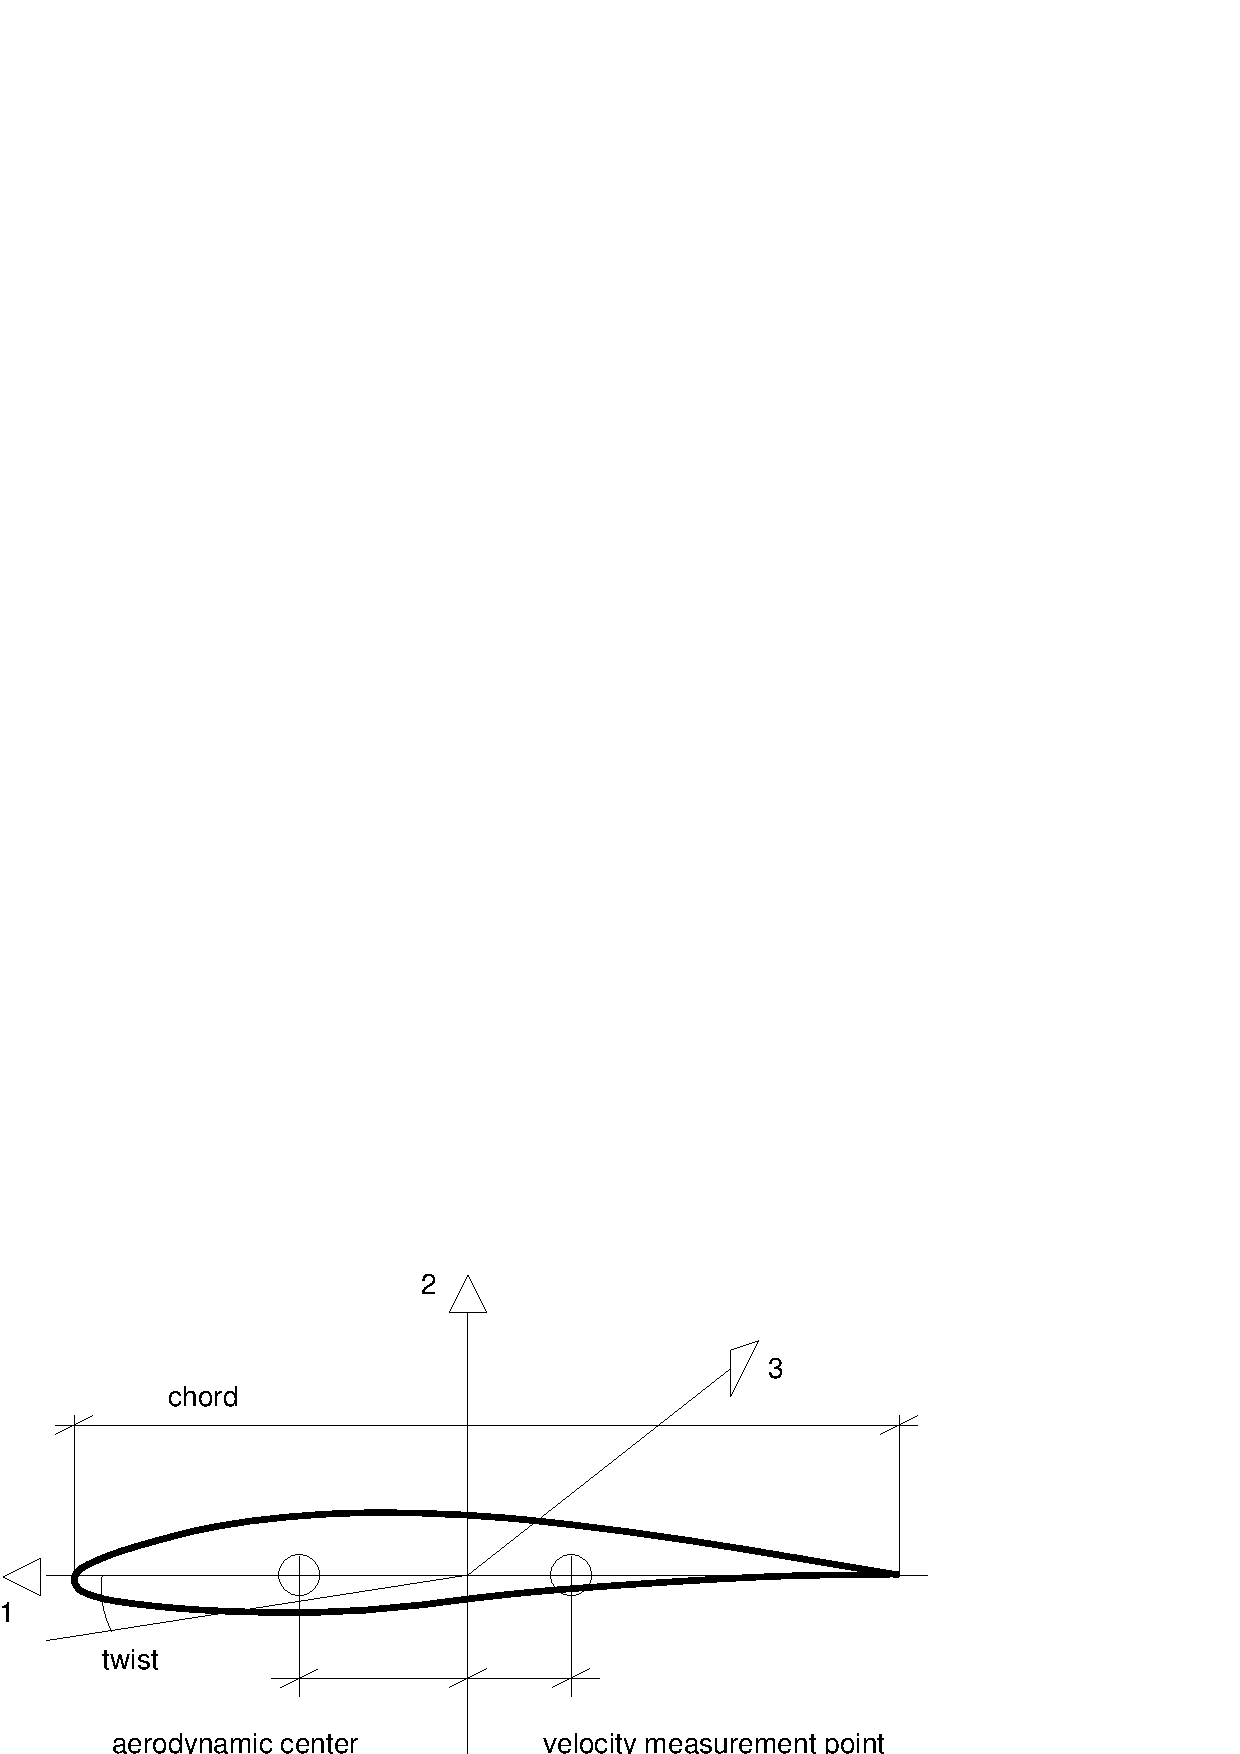
\includegraphics[width=80mm]{airfoil.pdf}
    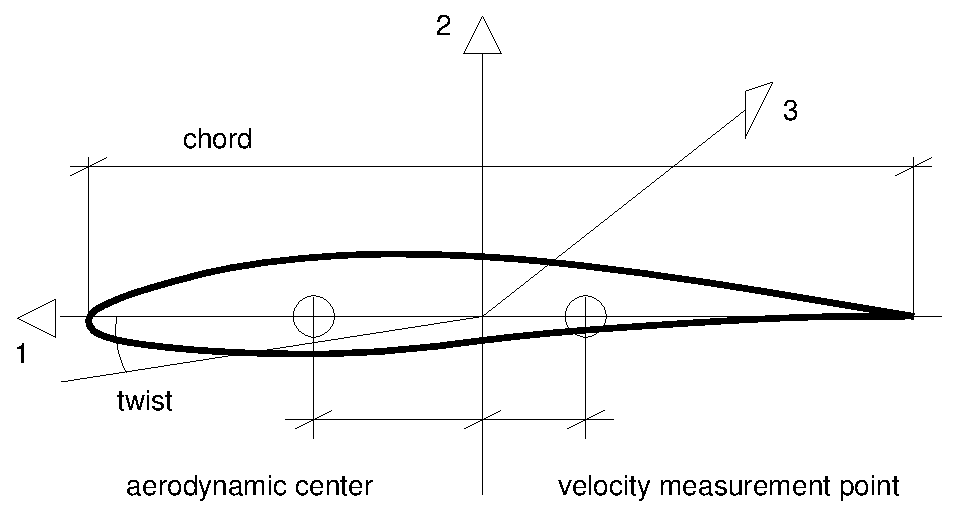
\includegraphics[width=80mm]{airfoil.eps}
  \caption{Airfoil geometry}\label{fig:AIRFOIL}
\end{figure}

The \kw{airfoil\_data} defaults to a builtin NACA 0012 semi-analytical
model (FIXME: the unsteady correction is buggy; use the \kw{c81} 
mode instead).

The \kw{multiple} mode of the c81 data allows to specify
more than one airfoil for an aerodynamic element; the transition
between airfoils is sharp.
The integer \kw{airfoil\_number} indicates how many airfoils are expected;
the real \kw{end\_point} indicates where the influence zone for that
airfoil ends, expressed in terms of a non-dimensional abscissa spanning 
$\plbr{-1,1}$ along the reference line, roughly along axis 3 
of the aerodynamic reference frame; \kw{end\_point} must not lie outside
the element.
So, for example, if airfoil NACA 0015 is used in the leftmost part
of an element up to 1/4 span, NACA 0012 is used from 1/4 to 3/4 span,
and NACA 0009 is used in the remaining rightmost 1/4, the syntax is:
\begin{verbatim}
    set: integer naca0015 = 15;
    set: integer naca0012 = 12;
    set: integer naca0009 = 9;
    c81 data: naca0015, "naca0015.c81";
    c81 data: naca0012, "naca0012.c81";
    c81 data: naca0009, "naca0009.c81";
    # beginning of aerodynamic element definition...
        multiple, 3,
            naca0015, -0.5,    # from -1.0 to -0.5
            naca0012,  0.5,    # from -0.5 to  0.5
            naca0009,  1.0,    # from  0.5 to  1.0
    # ...rest of aerodynamic element definition
\end{verbatim}

The \kw{interpolated} mode of the c81 data allows to specify 
a smooth transition between different airfoils inside an element.
The interpolation occurs at the integration points where the
aerodynamic data is required, and it is performed once for all
at the beginning of the analysis.
Since this operation is time consuming, and essentially unnecessary,
the interpolated data can be generated once for all with the utility
\kw{util/c81merge} once the position of the integration point is known,
and the \kw{multiple} mode can be used to directly provide
the interpolated data to the aerodynamic element.

\noindent
\emph{FIXME: not implemented yet}


\subsection{Output}
Aerodynamic elements, both bodies and beams, write their output with file
extension \kw{.aer}; for each time step the required elements are output.
Three different formats are available; the format can be selected only at
compile time, and it must be the same for all the elements. 

\noindent
\emph{Note: eventually it will freeze; if all the output formats will be
maintained, they will be made selectable at run-time.}

\noindent
In any case the label of the element is output first.

\subsubsection{Node}
The format is:
\begin{itemize}
    \item the label of the node
    \item the three components of the force applied to the node
    \item the three components of the couple applied to the node
\end{itemize}
When an \kw{aerodynamic beam} is considered, the output is repeated 
for each node the element is attached to.

\subsubsection{Forces at Gauss points}
The output refers to each Gauss integration point; the format is:
\begin{itemize}
    \item the direction of the wind velocity relative to the element frame
    \item the lift,
    \item the drag,
    \item and the aerodynamic moment per unit length
\end{itemize}
When an \kw{aerodynamic beam} is considered, the output 
is repeated for each portion of beam.

\subsubsection{Coefficients at Gauss points}
The output refers to each Gauss integration point; the format is:
\begin{itemize}
    \item the local incidence
    \item the local yaw angle
    \item the local Mach number
    \item the lift,
    \item the drag,
    \item and the aerodynamic moment coefficient
\end{itemize}
When an \kw{aerodynamic beam} is considered, the output 
is repeated for each portion of the beam.



\section{Aeromodal Element}
\emph{Note: prepared by Alessandro Scotti.}

\noindent
This element is used to model an aerodynamic modal element,
i.e.\ an unsteady aerodynamic model that inherits the structural 
motion from a  \htmlref{\kw{modal}}{sec:EL:STRUCT:JOINT:MODAL} element
Its definition is very similar to that of the pure modal element, 
but it also includes some data representing unsteady aerodynamics 
in the time domain trough the residualization matrices.
This element is defined as follows:
\begin{verbatim}
    <joint_type> ::= aeromodal
    <joint_arglist> ::= <label> , 
        <modal node> ,  
        <reference modal joint> ,
        (Mat3x3)<orientation> ,
        <reference chord> ,
        <number of aerodynamic states> ,
        <state space modal matrices file>
\end{verbatim}
With this formulation, anytime an aeromodal element is defined, 
the user needs to declare the number of modal aerodynamic elements 
in use in the \kw{control data} section.
An \htmlref{\kw{air properties}}{sec:EL:AERO:AIRPORPERTIES}
card definition is also required. 
The \kw{.fea} file includes the state space model in form 
of matrices $A$, $B$, $C$, $D_0$, $D_1$ and $D_2$, according to the representation
\begin{align*}
	\dot{\T{x}} &= \T{A}\T{x} + \T{B}\T{q} \\	
	\T{f} &= q\plbr{\T{C}\T{x} + \T{D}_0 \T{q} + \frac{2V_{\infty}}{c} \T{D}_1 \dot{\T{q}} + \plbr{\frac{2V_{\infty}}{c}}^2 \T{D}_2 \ddot{\T{q}}}
\end{align*}
where $\T{q}$ are the modal variables that describe the structural motion,
and $\T{f}$ are the unsteady aerodynamic forces that apply to the structural
dynamics equations.

The file is formatted as follows:
\begin{verbatim}
    *** MATRIX A
    (<na> x <na> coefficients)
    *** MATRIX B
    (<na> x <ns> coefficients)
    *** MATRIX C
    (<ns> x <na> coefficients)
    *** MATRIX D0
    (<ns> x <ns> coefficients)
    *** MATRIX D1
    (<ns> x <ns> coefficients)
    *** MATRIX D2
    (<ns> x <ns> coefficients)
\end{verbatim}

\noindent
Example:
\begin{verbatim}
    aeromodal: Wing, Wing, Wing,
        eye,
        131.25, 10, "ha145b.fea";
\end{verbatim}
The \kw{aeromodal} element is declared with the label \kw{Wing}.
This element is attached to a modal node, also labeled
with the name \kw{Wing}, and the reference \kw{modal} joint 
it is referred to is named \kw{Wing} as well.
The orientation of the aerodynamic reference with respect 
to the nodal reference is here expressed by the matrix eye.
The aerodynamic element chord is 131.25 (inches!).
This quantity must be consistent with the system chosen to define 
the whole model (S.I., for example; in this case, British Units).
The next field, 10, indicates the number of states needed to use 
the aerodynamic model.
The string \kw{ha145b.fea} is the name of the file that contains
the state space model matrices, obtained with an approximation 
chosen by the user.
In this particular case, a 10 states Pad\'e approximation 
has been chosen.
This example is taken from the Bisplinghoff Ashley Halfman
(BAH) Jet Transport Wing cantilevered wing with modal aerodynamic 
frequency responce, computed by a double-lattice method at Mach 0.0.
Data were extracted from the MSC-NASTRAN aeroelastic example file, 
named \kw{ha145b}, while the aerodynamic state-space fitting 
has been computed using a Pad\'e polynomial approximation
(by Pasinetti \& Mantegazza).
All quantities are expressed in inches and pounds.



\section{Aircraft Instruments}
\begin{verbatim}
    <card> ::= aircraft instruments
    <arglist> ::= <aircraft_node>
        [ , orientation , (Mat3x3)<relative orientation> ]
\end{verbatim}
The \kw{<aircraft\_node>} represents the aircraft; it is assumed
that the ``nose'' of the aircraft is toward the positive $x$ direction
of the node, and the ``top'' of the aircraft is toward the positive 
$z$ direction of the node.
An optional orientation can be added to change the orientation 
of the aircraft with respect to the node.
This is useful, for example, with helicopters, where conventionally
the positive direction of the $x$ axis is nose to tail.

The available measures are accessed during the simulation 
by defining appropriate \kw{parameter} nodes, and by binding
the \kw{aircraft instruments} element private data to the nodes 
by means of the \kw{bind} mechanism, or directly by means
of the 
\hyperref{\kw{element} drive}{\kw{element} drive (see Section~}{)}{sec:DRIVE-ELEMENT}.

\paragraph{Private Data}
The following data is available:
\begin{itemize}
\item \kw{"airspeed"} the airspeed as seen by the reference 
	point on the aircraft, i.e. the combination 
	of the airstream speed and of the node speed
\item \kw{"groundspeed"} the absolute value of the projection
	of the node speed in the $xy$ plane.
\item \kw{"altitude"} the $z$ component of the node position
\item \kw{"attitude"} $\arctan\plbr{r_{31}, r_{11}}$
	(FIXME: better $\arcsin\plbr{r_{31}}$?)
\item \kw{"bank"} $\arctan\plbr{r_{32}, r_{22}}$
	(FIXME: better $\arcsin\plbr{r_{32}}$?)
\item \kw{"turn"} (not available yet)
\item \kw{"slip"} (not available yet)
\item \kw{"verticalspeed"} the $z$ component of the node velocity
\item \kw{"angleofattack"} the angle between the $z$ 
\item \kw{"heading"} the angle between the $x$ axis of the aircraft 
	and the ``north'' (the global $x$ axis) about the global $z$ axis;
	note: heading wraps about South
	(+180 deg from East, -180 deg from West).
\end{itemize}

\noindent
\emph{Note: this element is eXperimental.}




\section{Air Properties Element}\label{sec:EL:AERO:AIRPORPERTIES}
The properties of the airstream are made of the physical properties
of the air plus the description of the airstream velocity direction
and amplitude.
The former can be expressed in different forms, while the latter
are based on three-dimensional vectors which depend on multipliers.
\begin{verbatim}
    <arglist> ::= {
        (drive_caller) <air_density> , (scalar) <sound_speed> 
        | std , { { SI | British }
            [ , temperature deviation , <delta T> ]
            | <p0> , (drive_caller) <rho0> ,
            <T0> , <dT/dz> , <R> , <g0> , <z1> , <z2>
        } [ , reference altitude, <z0> ]
    } , (Vec3_tpl_drive_caller) <air_speed>
    [ , gust , <gust_model> ]
\end{verbatim}
The first form consists in the bare input of the air density,
in form of a drive caller, and of the sound celerity, e.g.:
\begin{verbatim}
    air properties: 1.225, 340.,
        1.,0.,0., 150.;
\end{verbatim}
The second form uses standard air properties, both in the
international system (SI) or in British units, possibly
with a temperature deviation and an altitude offset, e.g.:
\begin{verbatim}
    air properties: std, SI, temperature deviation, -55,
        reference altitude, 1000.,
        1.,0.,0., 150.;
\end{verbatim}
where standard properties in SI are used, with a temperature
deviation of -55 K and a reference altitude of 1000 m.
The air properties are computed based on the Z position of the
point where the air properties are requested (plus the optional
altitude offset).
The last possibility lets the user input all the parameters
required to compute the air properties based on the Z position
of the point where they are requested, namely the reference
pressure \kw{p0}, the reference density \kw{rho0},
the reference temperature \kw{T0}, the initial temperature
gradient \kw{dT/dz}, the gas constant \kw{R}, the
initial gravity acceleration \kw{g0}, the bottom and top
altitudes of the null temperature gradient region \kw{z1} and
\kw{z2}; e.g., for SI units:
\begin{verbatim}
    air properties: std,
        101325.,       /* Pa */
        1.2250,        /* kg/m^3 */
        288.16,        /* K */
        -6.5e-3,       /* K/m */
        287.,          /* J/kgK */
        9.81,          /* m/s^2 */
        11000.,        /* m */
        25000.,        /* m */
        temperature deviation, -55,
        reference altitude, 1000.,
        1.,0.,0., 150.;
\end{verbatim}
The asymptotic air properties are characterized by the 3D template drive 
of the air speed, in the global reference frame.
If the optional \kw{gust} keyword is used, a gust model can be added.
Note that a very elementary gust model, represented by a uniform change
in airstream speed and direction can be implemented by using
a time-dependent airstream drive.
A more sophisticated model is currently available, and provisions are
made to allow four-dimensional gust profiles, dependent on time
and position.
The syntax is:
\begin{verbatim}
    <gust_model> ::= front 1D ,
        (Vec3) <front_direction> ,
        (Vec3) <perturbation_direction> ,
        (scalar) <front_velocity> ,
        (drive_caller) <front_profile>
\end{verbatim}
This model consists in a uniform front, defined as
\begin{displaymath}
	\T{v}\plbr{\T{x}, t} = \T{n} g\plbr{\T{f} \cdot \T{x} + V_{ref} \cdot t}
\end{displaymath}
where
\begin{itemize}
\item $\T{v}$ is the velocity perturbation;
\item $\T{x}$ is the position of the point whose airstream velocity
is being computed;
\item $t$ is the current time;
\item $\T{n}$ is the unit vector \kw{perturbation\_direction} 
that defines the direction of the velocity perturbation;
\item $g\plbr{\cdot}$ is the function \kw{front\_profile} 
that defines the gust profile;
\item $\T{f}$ is the unit vector \kw{front\_direction} 
that defines the direction of propagation of the front;
\item $V_{ref}$ is the velocity \kw{front\_velocity} 
of propagation of the front in direction $\T{f}$.
\end{itemize}
As an example, a transverse cosine-shaped gust, with a wavelength of 100 m
and a peak velocity of 5 m/s moving downstream at the airstream speed,
100 m/s, in standard air, is presented:
\begin{verbatim}
    set: real waveLength = 100.; # m
    set: real V_inf = 100.;      # m/s
    set: real V_g = 5.;          # m/s
    air properties: std, SI,
        1.,0.,0., const, V_inf,  # reference airstream along X
        gust, front 1D,
            1.,0.,0.,            # front moving along X
            0.,0.,1.,            # gust along Z
            V_inf,               # front moving at V_inf
            cosine, 0., pi/waveLength, V_g/2., one, 0.;
\end{verbatim}

\subsection{Output}
The output occurs in the \kw{.air} file, which contains:
\begin{itemize}
\item a fake label, always set to 0
\item the air density
\item the sound celerity
\item the three components of the reference air speed
with respect to the inertial reference frame
\end{itemize}



\section{Automatic structural}
The so called \kw{automatic structural} element is automatically generated
when a dynamic structural node is instantiated.
As such, when defined in the \kw{elements} block,
the element already exists.
The only reason to repeat its definition is to modify the values
of the momentum and of the momenta moment, and to initialize
their derivatives.
The label must match that of the node it refers to.
\begin{verbatim}
    <element_type> ::= beam3
    <normal_arglist> ::=
        (Vec3) <momentum> ,
        (Vec3) <momenta_moment> ,
        (Vec3) <momentum_derivative> ,
        (Vec3) <momenta_moment_derivative>
\end{verbatim}
All the provided values are recomputed during the initial derivatives phase,
so they should be intended as initial values for the Newton iteration.
In general, there is no need to provide this data; they can speed up
initial convergence in case of systems that are not at rest in the initial
configuration, with kinematic constraints that strongly affect
the motion.

\paragraph{Private Data}
The following data is available:
\begin{enumerate}
\item \kw{"beta[1]"} momentum in global direction 1
\item \kw{"beta[2]"} momentum in global direction 2
\item \kw{"beta[3]"} momentum in global direction 3
\item \kw{"gamma[1]"} momenta moment in global direction 1
\item \kw{"gamma[2]"} momenta moment in global direction 2
\item \kw{"gamma[3]"} momenta moment in global direction 3
\item \kw{"betaP[1]"} momentum derivative in global direction 1
\item \kw{"betaP[2]"} momentum derivative in global direction 2
\item \kw{"betaP[3]"} momentum derivative in global direction 3
\item \kw{"gammaP[1]"} momenta moment derivative in global direction 1
\item \kw{"gammaP[2]"} momenta moment derivative in global direction 2
\item \kw{"gammaP[3]"} momenta moment derivative in global direction 3
\end{enumerate}





\section{Beam Element}
The family of finite volume beam elements implemented in MBDyn
allows to model slender deformable structural components 
with a high level of flexibility.

\noindent
The beam is defined by a reference line and by a manifold
of orientations attached to the line.
It is assumed that the direction 1 of the orientations lies along
the reference line, but it is not strictly required to be tangent
to it even in the reference configuration.

\noindent
The beam element is defined by its nodes; currently, 2 and 3 node 
beam elements are implemented.
Each node of the beam is related to a \kw{structural node} by an offset
and a relative orientation, to provide topological flexibility.
The beam element is modeled by means of an original Finite Volume approach
\cite{FV-AIAA}, which computes the internal forces as functions 
of the straining of the reference line and orientation at selected points
along the line itself, called \emph{evaluation points},
which lie somewhere between two pairs of beam nodes.
At each evaluation point, a 6D constitutive law must be defined,
which defines the relationship between the strains, the curvatures
of the beam and their time derivatives
and the internal forces and moments at the evaluation points.
The strains and curvatures and their time derivatives are obtained 
from the nodal positions and orientations by differentiating
the interpolation functions.
The 6D constitutive laws are defined as
\begin{displaymath}
	\cubr{\cvvect{
		F_x \\
		F_y \\
		F_z \\
		M_x \\
		M_y \\
		M_z
	}} = \T{f}\plbr{
		\cubr{\cvvect{
			\varepsilon_x \\
			\gamma_y \\
			\gamma_z \\
			\kappa_x \\
			\kappa_y \\
			\kappa_z
		}},
		\cubr{\cvvect{
			\dot{\varepsilon}_x \\
			\dot{\gamma}_y \\
			\dot{\gamma}_z \\
			\dot{\kappa}_x \\
			\dot{\kappa}_y \\
			\dot{\kappa}_z
		}}
	}
\end{displaymath}
where, if the convention of using $x$ as beam axis is followed:
\begin{itemize}
\item $F_x$ is the axial force component;
\item $F_y$ and $F_z$ are the shear force components;
\item $M_x$ is the torsional moment component;
\item $M_y$ and $M_z$ are the bending moment components;
\item $\varepsilon_x$ is the axial strain component;
\item $\gamma_y$ and $\gamma_z$ are the shear strain components;
\item $\kappa_x$ is the torsional curvature component;
\item $\kappa_y$ and $\kappa_z$ are the bending curvature component;
\item $\T{f}$ is an arbitrary function that defines the constitutive law.
\end{itemize}



\subsection{Beam Section Constitutive Law}
Typically, linear elastic or viscoelastic constitutive laws are used,
although one may want to implement specific nonlinear elastic
or elastic-plastic constitutive laws.



\subsubsection{Beam Section Characterization}
MBDyn allows the broadest generality in defining what a linear elastic 
constitutive law contains, since the entire $6\times{6}$ constitutive
matrix can be input.
This means that internal forces and couples can be arbitrarily related
to generalized strains and curvatures.
However, to make sense, a constitutive matrix at the section level,
must satisfy some constraints, e.g.\ it is expected to be symmetric, 
although this is not strictly enforced by the code.

However, most of the info about the extra-diagonal terms 
of the stiffness matrix are not usually available.
One easy way to work this around is to resort to any so-called
composite beam section characterization analysis available 
in the literature.
For details, the reader is referred to \cite{HODGES-REVIEW90} 
for a review of the topic, to \cite{ANBA-GIAVOTTO-83}
for an early work on the subject, and to \cite{MASARATI-2001}
for a recent review of the original formulation.


\subsubsection{Disclaimer}
The following paragraphs are intended as a means to help users
preparing data for MBDyn models in a consistent manner.
By no means they indicate that the beam section stiffness properties
must be provided in a specific reference frame.
On the contrary, MBDyn allows as much generality as possible,
and actually the variety of choices is redundant, since equivalent
properties can be input in different ways.
This is intended to allow the code to suit the user's needs
regardless of the original format of the input data.
As such, all the transformations reported in the following 
are only intended as suggestions and should not be taken literally.
For instance, rotations and transportation of reference points
could be reversed, changing the values of the offsets, without
affecting the final result.
The most important aspect of MBDyn notion of beam section properties
is that the reference point and orientation, although arbitrary,
must be unique, and the common notions of center of axial strain,
shear center (and center of mass) have no special meaning.



\subsubsection{Equivalent $6\times6$ Section of Isotropic Beam}
When an isotropic beam section is considered, the $6\times$ 
constitutive matrix, referred to an arbitrary point in the section,
with an arbitrary orientation, can always be written in terms 
of elementary stiffness and geometrical properties.
These are the properties that are usually available in tabular form
either from simplified beam section analysis or by experiments.
A sketch of a generic section is shown
in Figure~\ref{fig:EL:BEAM:SECTION},
where the arbitrary reference frame indicated by axes 
$x$, $y$ and $z$ originates from an arbitrary reference point
on the section.

Isotropic uniform beam sections allow to group the internal forces 
and couples in two sets, together with their conjugated generalized 
strains:
those related to shear stress and strain, and those related 
to axial stress and strain, as illustrated
in Figure~\ref{fig:EL:BEAM:GROUPS}.
\begin{figure}[h]
\centering
\begin{tabular}{c|c|c|c|c|c|c|}
	&
		$\varepsilon_x$ &
		$\gamma_y$ &
		$\gamma_z$ &
		$\kappa_x$ &
		$\kappa_y$ &
		$\kappa_z$ \\
	\hline
	$F_x$ & A &   &   &   & A & A \\
	\hline
	$F_y$ &   & S & S & S &   &   \\
	\hline
	$F_z$ &   & S & S & S &   &   \\
	\hline
	$M_x$ &   & S & S & S &   &   \\
	\hline
	$M_y$ & A &   &   &   & A & A \\
	\hline
	$M_z$ & A &   &   &   & A & A \\
	\hline
\end{tabular}
\caption{Constitutive coefficients grouping (S: shear, A: axial)}
\label{fig:EL:BEAM:GROUPS}
\end{figure}
There is no direct coupling between the two group, at the section level,
so the corresponding coupling coefficients are always zero.
This is no longer true when material anisotropy must be taken 
into account.

The $3\times3$ sub-blocks can be separately transformed 
in diagonal form by referring the corresponding properties
to appropriate separate points in the beam section, 
and by applying an appropriate rotation about the axis of the beam.



\subsubsection{Axial Stress and Strain Properties}
Consider first the submatrix represented by the coefficients 
marked as A in Figure~\ref{fig:EL:BEAM:GROUPS}, under the assumption 
that it is symmetric, as indicated in Equation~(\ref{eq:EL:BEAM:AXIAL}):
\begin{equation}
	\cubr{\cvvect{
		F_x \\
		M_y \\
		M_z
	}} = \sqbr{\matr{ccc}{
		A_{11} & A_{12} & A_{13} \\
		 & A_{22} & A_{23} \\
		\llk{sym.} & & A_{33}
	}}\cubr{\cvvect{
		\varepsilon_x \\
		\kappa_y \\
		\kappa_z
	}}
	\label{eq:EL:BEAM:AXIAL}
\end{equation}
The transformation of Equation~(\ref{eq:EL:BEAM:AXIAL-TRANSFORM})
moves the point of application of the axial force 
of an arbitrary amount $\cubr{y,z}$ in the beam section, to the point
indicated as $as$ (axial strain) in Figure~\ref{fig:EL:BEAM:SECTION}:
\begin{eqnarray}
	\cubr{\cvvect{
		F_x \\
		M_y \\
		M_z
	}}^*
	& = & \sqbr{T_{\llk{axial}}}\cubr{\cvvect{
		F_x \\
		M_y \\
		M_z
	}}
	\nonumber \\
	& = & \sqbr{\matr{ccc}{
		 1 & 0 & 0 \\
		 z & 1 & 0 \\
		-y & 0 & 1
	}}\cubr{\cvvect{
		F_x \\
		M_y \\
		M_z
	}}
	\label{eq:EL:BEAM:AXIAL-TRANSFORM}
\end{eqnarray}
So the transformed axial block of the constitutive matrix becomes
\begin{eqnarray}
	\cubr{\cvvect{
		F_x \\
		M_y \\
		M_z
	}}^*
	& = & \sqbr{T_{\llk{axial}}}
	\cubr{\cvvect{
		F_x \\
		M_y \\
		M_z
	}}
	\nonumber \\
	& = & \sqbr{T_{\llk{axial}}} \sqbr{A} \sqbr{T_{\llk{axial}}}^T
	\cubr{\cvvect{
		\varepsilon_x \\
		\kappa_y \\
		\kappa_z
	}}^*
	\label{eq:EL:BEAM:AXIAL-TRANSFORMED}
	\\
	& = &
	\sqbr{\matr{ccc}{
		A_{11} & A_{12} + z A_{11} & A_{13} - y A_{11} \\
		& A_{22} + 2 z A_{12} + z^2 A_{11} & 
			A_{23} + z A_{13} - y A_{12} - yz A_{11} \\
		\llk{sym.} &  & A_{33} - 2 y A_{13} + y^2 A_{13}
	}}\cubr{\cvvect{
		\varepsilon_x \\
		\kappa_y \\
		\kappa_z
	}}^*
	\nonumber
\end{eqnarray}
If the position of the point is selected in such a manner 
that the axial force and the bending moment are decoupled, i.e.,
according to the definition of center of axial strain,
\begin{eqnarray*}
	y & = & \frac{A_{13}}{A_{11}} \\
	z & = & -\frac{A_{12}}{A_{11}}
\end{eqnarray*}
the axial block becomes
\begin{eqnarray*}
	\cubr{\cvvect{
		F_x \\
		M_y \\
		M_z
	}}^*
	& = &
	\sqbr{\matr{ccc}{
		A_{11} & 0 & 0 \\
		& A_{22} - A_{12}^2/A_{11} & A_{23} - A_{12}A_{13}/A_{11} \\
		\llk{sym.} &  & A_{33} - A_{13}^2/A_{11}
	}}\cubr{\cvvect{
		\varepsilon_x \\
		\kappa_y \\
		\kappa_z
	}}^*
	\\
	& = &
	\sqbr{\matr{ccc}{
		A_{11}^* & 0 & 0 \\
		& A_{22}^* & A_{23}^* \\
		\llk{sym.} &  & A_{33}^*
	}}\cubr{\cvvect{
		\varepsilon_x \\
		\kappa_y \\
		\kappa_z
	}}^*
\end{eqnarray*}
Now, a rotation about the beam section axis can be applied 
in order to decouple the bending moments:
\begin{eqnarray}
	\cubr{\cvvect{
		F_x \\
		M_y \\
		M_z
	}}^{\dagger}
	& = & \sqbr{R_{\llk{axial}}}\cubr{\cvvect{
		F_x \\
		M_y \\
		M_z
	}}^*
	\nonumber \\
	& = & \sqbr{\matr{ccc}{
		 1 & 0 & 0 \\
		 0 & \cos\alpha & -\sin\alpha \\
		 0 & \sin\alpha & \cos\alpha
	}}\cubr{\cvvect{
		F_x \\
		M_y \\
		M_z
	}}^*
	\label{eq:EL:BEAM:AXIAL-ROTATION}
\end{eqnarray}
The angle that decouples the bending moments is
\begin{equation*}
	\alpha = \frac{1}{2}\llk{atan}\plbr{\frac{2 A_{23}^*}{A_{22}^* - A_{33}^*}}
\end{equation*}
representing a rotation about the beam axis $x$ at point $as$
(axial strain) in Figure~\ref{fig:EL:BEAM:SECTION},
and the resulting coefficients are
\begin{eqnarray}
	EA & = & A_{11} \\
	EJ_y & = & A_{22}^* \cos^2\alpha + A_{33}^* \sin^2\alpha
		- 2 A_{23}^* \sin\alpha \cos\alpha \\
	EJ_z & = & A_{22}^* \sin^2\alpha + A_{33}^* \cos^2\alpha
		+ 2 A_{23}^* \sin\alpha \cos\alpha
\end{eqnarray}
When the axial and bending stiffnesses, and the position 
of the axial strain center and the orientation of the neutral axes
are available, the axial portion of the stiffness matrix 
can be computed by reversing the order of the transformations 
described in
Equations~(\ref{eq:EL:BEAM:AXIAL-TRANSFORM}--\ref{eq:EL:BEAM:AXIAL-ROTATION}),
i.e.:
\begin{equation}
	\sqbr{\matr{ccc}{
		A_{11} & A_{12} & A_{13} \\
		& A_{22} & A_{23} \\
		\llk{sym.} & & A_{33}
	}} = \sqbr{T_{\llk{axial}}}^{-1} \sqbr{R_{\llk{axial}}}^T \sqbr{\matr{ccc}{
		EA & 0 & 0 \\
		0 & EJ_y & 0 \\
		0 & 0 & EJ_z
	}} \sqbr{R_{\llk{axial}}} \sqbr{T_{\llk{axial}}}^{-T}
	\label{eq:EL:BEAM:AXIAL-TRANSFORM-REVERSED}
\end{equation}
This expression implies that the stiffness properties are referred
to an arbitrary point at $\cubr{-y,-z}$ from the axial strain center,
after that they are rotated into the section reference frame, 
i.e.\ by an amount $-\alpha$.
The resulting coefficients are
\begin{eqnarray*}
	A_{11} & = & EA \\
	A_{12} & = & -z EA \\
	A_{13} & = & y EA \\
	A_{22} & = & EJ_y \cos^2\alpha + EJ_z \sin^2\alpha + z^2 EA \\
	A_{23} & = & \plbr{EJ_z - EJ_y} \sin\alpha\cos\alpha - y z EA \\
	A_{33} & = & EJ_z \cos^2\alpha + EJ_y \sin^2\alpha + y^2 EA
\end{eqnarray*}



\subsubsection{Shear Stress and Strain Properties}
Consider now the submatrix represented by the coefficients 
marked as S in Figure~\ref{fig:EL:BEAM:GROUPS}, under the assumption 
that it is symmetric, as indicated in Equation~(\ref{eq:EL:BEAM:SHEAR}):
\begin{equation}
	\cubr{\cvvect{
		F_y \\
		F_z \\
		M_x
	}} = \sqbr{\matr{ccc}{
		S_{11} & S_{12} & S_{13} \\
		 & S_{22} & S_{23} \\
		\llk{sym.} & & S_{33}
	}}\cubr{\cvvect{
		\gamma_y \\
		\gamma_z \\
		\kappa_x
	}}
	\label{eq:EL:BEAM:SHEAR}
\end{equation}
The orientation of the shear force components about the section axis
can be selected in order to decouple them; by applying the transformation
\begin{eqnarray}
	\cubr{\cvvect{
		F_y \\
		F_z \\
		M_x
	}}^{\dagger}
	& = & \sqbr{R_{\llk{axial}}}\cubr{\cvvect{
		F_y \\
		F_z \\
		M_x
	}}^*
	\nonumber \\
	& = & \sqbr{\matr{ccc}{
		\cos\beta & -\sin\beta & 0 \\
		\sin\beta & \cos\beta & 0 \\
		0 & 0 & 1
	}}\cubr{\cvvect{
		F_y \\
		F_z \\
		M_x
	}}^*
	\label{eq:EL:BEAM:SHEAR-ROTATION}
\end{eqnarray}
The angle that decouples the shear forces is
\begin{equation*}
	\beta = \frac{1}{2}\llk{atan}\plbr{\frac{2 S_{12}^*}{S_{22}^* - S_{11}^*}}
\end{equation*}
representing a rotation about the axis $x$ of the beam with respect
to the origin of the initial reference frame as shown 
in Figure~\ref{fig:EL:BEAM:SECTION},
and the resulting coefficients are
\begin{eqnarray}
	GA_y & = & S_{11}^* \cos^2\alpha + S_{22}^* \sin^2\alpha
		- 2 S_{12}^* \sin\alpha \cos\alpha \\
	GA_z & = & S_{11}^* \sin^2\alpha + S_{22}^* \cos^2\alpha
		+ 2 S_{12}^* \sin\alpha \cos\alpha
\end{eqnarray}
the shear block becomes
\begin{eqnarray*}
	\cubr{\cvvect{
		F_y \\
		F_x \\
		M_x
	}}^*
	& = &
	\sqbr{\matr{ccc}{
		GA_y & 0 & S_{13}\cos\beta - S_{23}\sin\beta \\
		& GA_z & S_{13}\sin\beta + S_{23}\cos\beta \\
		\llk{sym.} &  & S_{33}
	}}\cubr{\cvvect{
		\gamma_y \\
		\gamma_z \\
		\kappa_x
	}}^*
	\\
	& = &
	\sqbr{\matr{ccc}{
		GA_y & 0 & S_{13}^* \\
		& GA_z & S_{23}^* \\
		\llk{sym.} &  & S_{33}
	}}\cubr{\cvvect{
		\gamma_y \\
		\gamma_z \\
		\kappa_x
	}}^*
\end{eqnarray*}
The transformation of Equation~(\ref{eq:EL:BEAM:SHEAR-TRANSFORM})
moves the point of application of the shear force 
of an arbitrary amount $\cubr{y,z}$ in the beam section,
with respect to the reference frame rotated by $\beta$ about 
the axis $x$ of the beam, as indicated
in Figure~\ref{fig:EL:BEAM:SECTION}:
\begin{eqnarray}
	\cubr{\cvvect{
		F_y \\
		F_z \\
		M_x
	}}^{\dagger}
	& = & \sqbr{T_{\llk{shear}}}\cubr{\cvvect{
		F_y \\
		F_z \\
		M_x
	}}^*
	\nonumber \\
	& = & \sqbr{\matr{ccc}{
		1 &  0 & 0 \\
		0 &  1 & 0 \\
		z & -y & 1
	}}\cubr{\cvvect{
		F_y \\
		F_z \\
		M_x
	}}^*
	\label{eq:EL:BEAM:SHEAR-TRANSFORM}
\end{eqnarray}
So the transformed shear block of the constitutive matrix becomes
\begin{eqnarray}
	\cubr{\cvvect{
		F_y \\
		F_z \\
		M_x
	}}^{\dagger}
	& = & \sqbr{T_{\llk{shear}}}
	\cubr{\cvvect{
		F_y \\
		F_z \\
		M_x
	}}^*
	\nonumber \\
	& = & \sqbr{T_{\llk{shear}}} \sqbr{A} \sqbr{T_{\llk{shear}}}^T
	\cubr{\cvvect{
		\gamma_y \\
		\gamma_z \\
		\kappa_x
	}}^{\dagger}
	\label{eq:EL:BEAM:SHEAR-TRANSFORMED}
	\\
	& = &
	\sqbr{\matr{ccc}{
		GA_y & 0 & S_{13}^* + z GA_y \\
		& GA_z & S_{23}^* - y GA_z \\
		\llk{sym.} &  & S_{33} - y S_{23}^* + z S_{13}^*
		+z\plbr{S_{13}^* + z GA_y} - y\plbr{S_{23}^* - y GA_z}
	}}\cubr{\cvvect{
		\gamma_y \\
		\gamma_z \\
		\kappa_x
	}}^{\dagger}
	\nonumber
\end{eqnarray}
If the position of the point is selected in such a manner 
that the shear force and the torsional moment are decoupled, i.e.,
according to the definition of center of shear force (the point 
in a beam section where the application of a transverse force
results in no twist)
\begin{eqnarray*}
	y & = & -\frac{S_{13}^*}{GA_y} \\
	z & = & \frac{S_{23}^*}{GA_z}
\end{eqnarray*}
the shear block becomes
\begin{eqnarray*}
	\cubr{\cvvect{
		F_y \\
		F_x \\
		M_x
	}}^{\dagger}
	& = &
	\sqbr{\matr{ccc}{
		GA_y & 0 & 0 \\
		& GA_z & 0 \\
		\llk{sym.} &  & S_{33} - {S_{13}^*}^2/GA_y - {S_{23}^*}^2/GA_z
	}}\cubr{\cvvect{
		\gamma_y \\
		\gamma_z \\
		\kappa_x
	}}^{\dagger}
	\\
	& = &
	\sqbr{\matr{ccc}{
		GA_y & 0 & 0 \\
		& GA_z & 0 \\
		\llk{sym.} &  & GJ
	}}\cubr{\cvvect{
		\gamma_y \\
		\gamma_z \\
		\kappa_x
	}}^{\dagger}
\end{eqnarray*}
When the shear and torsional stiffnesses, and the position 
of the shear strain center and the orientation of the shear axes
are available, the shear portion of the stiffness matrix 
can be computed by reversing the order of the transformations 
described in
Equations~(\ref{eq:EL:BEAM:SHEAR-ROTATION}--\ref{eq:EL:BEAM:SHEAR-TRANSFORM}),
i.e.:
\begin{equation}
	\sqbr{\matr{ccc}{
		S_{11} & S_{12} & S_{13} \\
		& S_{22} & S_{23} \\
		\llk{sym.} & & S_{33}
	}} = \sqbr{R_{\llk{shear}}}^T \sqbr{T_{\llk{shear}}}^{-1} \sqbr{\matr{ccc}{
		GA_y & 0 & 0 \\
		0 & GA_z & 0 \\
		0 & 0 & GJ
	}} \sqbr{T_{\llk{shear}}}^{-T} \sqbr{R_{\llk{shear}}}
	\label{eq:EL:BEAM:SHEAR-TRANSFORM-REVERSED}
\end{equation}
This expression implies that the stiffness properties are referred
to an arbitrary point at $\cubr{-y,-z}$ from the shear center,
in the shear reference frame, followed by a rotation
into the section reference frame by an amount $-\beta$.
The resulting coefficients are
\begin{eqnarray*}
	S_{11} & = & GA_y \cos^2\beta + GA_z \sin^2\beta \\
	S_{12} & = & \plbr{GA_z - GA_y} \sin\beta\cos\beta \\
	S_{13} & = & y GA_z \sin\beta - z GA_y \cos\beta \\
	S_{22} & = & GA_z \cos^2\beta + GA_y \sin^2\beta \\
	S_{23} & = & y GA_z \cos\beta + z GA_y \sin\beta \\
	S_{33} & = & GJ + z^2 GA_y + y^2 GA_z
\end{eqnarray*}
Note that the order of the rotation and reference point transportation 
is reversed with respect to the axial properties; this is mostly done
for convenience in computing the coefficients, because the opposite
would result in more complicated formulas; however, their development
the other way 'round is straightforward.

\begin{figure}
\centering
\psfrag{alpha}{\hspace{0cm}\large $\alpha$}
\psfrag{beta}{\hspace{0cm}\large $\beta$}
\psfrag{sc}{\hspace{0cm}\large s.c.}
\psfrag{a.s.}{\hspace{0cm}\large a.s.}
\psfrag{x}{\hspace{0cm}\large $x$}
\psfrag{y}{\hspace{0cm}\large $y$}
\psfrag{z}{\hspace{0cm}\large $z$}
\psfrag{ysc}{\hspace{0cm}\large $y_{sc}$}
\psfrag{zsc}{\hspace{0cm}\large $z_{sc}$}
\psfrag{yas}{\hspace{0cm}\large $y_{as}$}
\psfrag{zas}{\hspace{0cm}\large $z_{as}$}
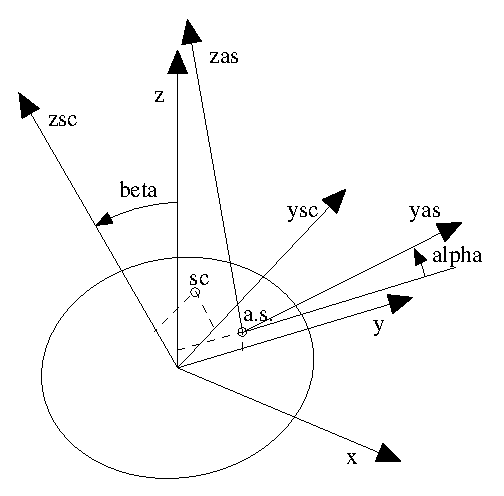
\includegraphics[width=.7\textwidth]{beamsect}
\caption{Beam section}
\label{fig:EL:BEAM:SECTION}
\end{figure}



\subsubsection{Locking Correction for Two-Node Beam}
The three-node finite volume element has been implemented first, 
and uses conventional polynomial parabolic interpolation 
of the nodal displacements and orientations;
the two-node finite volume element has been introduced later.
This latter element presents some shear-locking, which, for linear elastic
constitutive laws, may be overcome by correcting the section stiffness matrix
in a relatively straightforward form:
\begin{equation}\label{eq:2-NODE-BEAM-STIFFNESS}
	\hat{\T{K}} = \plbr{\T{F} + \frac{L^2}{12}\T{T} \T{F} \T{T}^T}^{-1} ,
\end{equation}
where $\T{F}=\T{K}^{-1}$ is the compliance matrix of the section, 
$L$ is the length of the beam, i.e.\ the distance between
the two reference points obtained by adding the optional offset 
to the nodes, and
\begin{displaymath}
	\T{T} \ = \ \sqbr{\matr{cc}{
		\T{0} & \T{e}_x \times{} \\
		\T{0} & \T{0}
	}}
\end{displaymath}
is the ``arm'' matrix that appears in the differential equilibrium equation
\begin{displaymath}
	\T{\vartheta}_{/x} - \T{T}^T\vartheta + \T{f} \ = \ 0 .
\end{displaymath}
There are no provisions to automatically apply the correction 
when defining the constitutive law of the section.
The two-node beam has been reimplemented using a helicoidal interpolation
of the nodal positions and orientations, to improve its capability
to undergo large displacements and relative rotations.
It is activated by using the keyword \kw{hbeam2} instead of \kw{beam2}.
However, to reduce the shear-locking effect, the stiffness properties 
still need to be manually corrected according
to Equation~(\ref{eq:2-NODE-BEAM-STIFFNESS}).
The \kw{hbeam2} element is \emph{experimental}, and should be used
only for development purposes.


\subsection{Three-node beam element}
The three node beam element is described in detail in \cite{FV-AIAA}.
Each ``node'' is referred to a structural node but can have an arbitrary
offset to allow high generality in the positioning of the structural 
reference line of the beam.
A finite volume formulation is used;
as a consequence, the internal forces and moments are evaluated 
at two points that are at about midpoint between nodes 1 and 2, 
and nodes 2 and 3 (at $ -1/\sqrt{3} $ and $1/\sqrt{3}$ considering
a non-dimensional abscissa running from -1 at node 1 to 1 at node 3).
So the constitutive properties must be supplied in these points, as well as
the orientation matrices from the material to the global frame (the axial force
is in direction 1).
Any of the allowed 6D constitutive laws can be supplied to define the
constitutive properties.
The traditional input format is
\begin{verbatim}
    <element_type> ::= beam3
    <normal_arglist> ::=
        <node_1> , (Vec3) <relative_offset_1> ,
        <node_2> , (Vec3) <relative_offset_2> ,
        <node_3> , (Vec3) <relative_offset_3> ,
        (OrientationMatrix) <orientation_matrix_section_I> ,
        (ConstitutiveLaw6D) <constitutive_law_section_I> ,
        { same | (OrientationMatrix) <orientation_matrix_section_II> } ,
        { same | (ConstitutiveLaw6D) <constitutive_law_section_II> }
\end{verbatim}
Based on the type of constitutive law, the simple or the viscoelastic beam
element is used.
The two keywords \kw{same} respectively mean that the same orientation 
and the same constitutive law defined for the first point will be used 
for the second point.
A more complete input format is
\begin{verbatim}
    <element_type> ::= beam3
    <normal_arglist> ::=
        <node_1> ,
            [ position , ] (Vec3) <relative_offset_1> ,
            [ orientation , (Mat3x3) <relative_orientation_1> , ]
        <node_2> ,
            [ position , ] (Vec3) <relative_offset_2> ,
            [ orientation , (Mat3x3) <relative_orientation_2> , ]
        <node_3> ,
            [ position , ] (Vec3) <relative_offset_3> ,
            [ orientation , (Mat3x3) <relative_orientation_3> , ]
        { (OrientationMatrix) <orientation_matrix_section_I>
            | from nodes } ,
        (ConstitutiveLaw6D) <constitutive_law_section_I> ,
        { same
            | (OrientationMatrix) <orientation_matrix_section_II>
            | from nodes } ,
        { same
            | (ConstitutiveLaw6D) <constitutive_law_section_II> }
\end{verbatim}
This format is a superset of the traditional one, which is extended
by adding the possibility to set relative node orientations
that can be subsequently used to interpolate the orientation matrices
at the evaluation points, by providing the keyword \kw{from nodes}
instead of the matrix.
If the keyword \kw{same} is used for the second evaluation point,
the same method is used to compute the orientation matrix.

\noindent
As an example, a simple beam element, with diagonal section stiffness 
matrix is presented:
\begin{verbatim}
    set: integer beam_label = 1000;
    set: integer beam_node1 = 2001;
    set: integer beam_node2 = 2002;
    set: integer beam_node3 = 2003;
    set: real EA = 1e6;   # N
    set: real GAy = .6e6; # N
    set: real GAy = .6e6; # N
    set: real GJ = 1.e3;  # Nm^2
    set: real EJy = 2.e3; # Nm^2
    set: real EJz = 1.e4; # Nm^2
    beam3: beam_label,
        beam_node1, reference, node, null,
        beam_node2, reference, node, null,
        beam_node3, reference, node, null,
        eye,
        linear elastic generic, diag,
            EA, GAy, GAz, GJ, EJy, EJz,
        same,
        same;
\end{verbatim}

\noindent
A not-so-simple beam section, where the center of axial strain 
and the shear center are not coincident, is illustrated below.
The node offset is used to align the reference line 
with the shear center, and the axial strain center offset 
is used in the constitutive matrix:
\begin{verbatim}
    set: integer beam_label = 1000;
    set: integer beam_node1 = 2001;
    set: integer beam_node2 = 2002;
    set: integer beam_node3 = 2003;
    set: real EA = 1e6;    # N
    set: real GAy = .6e6;  # N
    set: real GAy = .6e6;  # N
    set: real GJ = 1.e3;   # Nm^2
    set: real EJy = 2.e3;  # Nm^2
    set: real EJz = 1.e4;  # Nm^2
    set: real yas = 2.e-2; # m
    set: real zas = 1.e-2; # m
    set: real ysc = 4.e-2; # m
    set: real zsc = 2.e-2; # m
    set: real y = yas-ysc; # compute the axial strain center
    set: real z = zas-zsc; # wrt/ the shear center
    beam3: beam_label,
        beam_node1, reference, node, 0.,ysc,zsc,
        beam_node2, reference, node, 0.,ysc,zsc,
        beam_node3, reference, node, 0.,ysc,zsc,
        eye,
        linear elastic generic, sym,
            EA, 0.,  0.,  0., z*EA,       -y*EA,
                GAy, 0.,  0., 0.,          0.,
                     GAz, 0., 0.,          0.,
                          GJ, 0.,          0.,
                              EJy+z^2*EA, -z*y*EA,
                                           EJz+y^2*EA,
        same,
        same;
\end{verbatim}


\noindent
A piezoelectric actuator beam element is available; an arbitrary
linear piezoelectric actuation matrix is required, together with the labels
of the abstract nodes that represent the input signal tensions, as follows:
\begin{verbatim}
    <normal_arglist> ::=
        <node_1> , (Vec3) <relative_offset_1> ,
        <node_2> , (Vec3) <relative_offset_2> ,
        <node_3> , (Vec3) <relative_offset_3> ,
        (OrientationMatrix) <orientation_matrix_section_I> ,
        (ConstitutiveLaw6D) <constitutive_law_section_I> ,
        { same | (OrientationMatrix) <orientation_matrix_section_II> } ,
        { same | (ConstitutiveLaw6D) <constitutive_law_section_II> } ,
        piezoelectric actuator , 
        <electrodes_number> ,
        <abstract_node_label_list> ,
        (Mat6xN) <piezoelectric_matrix_I> ,
        { same | (Mat6xN) <piezoelectric_matrix_II> }
\end{verbatim}
where the \kw{abstract\_node\_label\_list} is the list of the labels of the
abstract nodes that represent the electrodes.


\paragraph{Private Data}
The following data is available:
\begin{enumerate}
\item \kw{"pI.ex"} point I axial strain
\setcounter{enumi}{3}
\item \kw{"pI.kx"} point I curvature about local axis 1 (torsional)
\item \kw{"pI.ky"} point I curvature about local axis 2 (bending)
\item \kw{"pI.kz"} point I curvature about local axis 3 (bending)
\item \kw{"pI.Fx"} point I axial force
\setcounter{enumi}{9}
\item \kw{"pI.Mx"} point I moment about local axis 1 (torsional)
\item \kw{"pI.My"} point I moment about local axis 2 (bending)
\item \kw{"pI.Mz"} point I moment about local axis 3 (bending)
\item \kw{"pII.ex"} point II axial strain
\setcounter{enumi}{15}
\item \kw{"pII.kx"} point II curvature about local axis 1 (torsional)
\item \kw{"pII.ky"} point II curvature about local axis 2 (bending)
\item \kw{"pII.kz"} point II curvature about local axis 3 (bending)
\item \kw{"pII.Fx"} point II axial force
\setcounter{enumi}{21}
\item \kw{"pII.Mx"} point II moment about local axis 1 (torsional)
\item \kw{"pII.My"} point II moment about local axis 2 (bending)
\item \kw{"pII.Mz"} point II moment about local axis 3 (bending)
\end{enumerate}









\subsection{Two-node beam element}
\begin{verbatim}
    <element_type> ::= beam2
    <normal_arglist> ::=
        <node_1> , (Vec3) <relative_offset_1> ,
        <node_2> , (Vec3) <relative_offset_2> ,
        (OrientationMatrix) <orientation_matrix_section_I> ,
        (ConstitutiveLaw6D) <constitutive_law_section_I>
        [ , piezoelectric actuator , 
        <electrodes_number> ,
        <abstract_node_label_list> ,
        (Mat6xN) <piezoelectric_matrix_I> ]
\end{verbatim}
\begin{verbatim}
    <element_type> ::= beam2
    <normal_arglist> ::=
        <node_1> ,
            [ positions , ] (Vec3) <relative_offset_1> ,
            [ orientation , (Mat3x3) <relative_orientation_1> , ]
        <node_2> ,
            [ positions , ] (Vec3) <relative_offset_2> ,
            [ orientation , (Mat3x3) <relative_orientation_2> , ]
        { (OrientationMatrix) <orientation_matrix_section_I>
            | from nodes } ,
        (ConstitutiveLaw6D) <constitutive_law_section_I>
        [ , piezoelectric actuator , 
        <electrodes_number> ,
        <abstract_node_label_list> ,
        (Mat6xN) <piezoelectric_matrix_I> ]
\end{verbatim}

\paragraph{Private Data}
The following data is available:
\begin{enumerate}
\item \kw{"ex"} axial strain
\setcounter{enumi}{3}
\item \kw{"kx"} curvature about local axis 1 (torsional)
\item \kw{"ky"} curvature about local axis 2 (bending)
\item \kw{"kz"} curvature about local axis 3 (bending)
\item \kw{"Fx"} axial force
\setcounter{enumi}{9}
\item \kw{"Mx"} moment about local axis 1 (torsional)
\item \kw{"My"} moment about local axis 2 (bending)
\item \kw{"Mz"} moment about local axis 3 (bending)
\end{enumerate}




As an example, a simple beam element, with diagonal section stiffness 
matrix is presented:
\begin{verbatim}
    set: integer beam_label = 1000;
    set: integer beam_node1 = 2001;
    set: integer beam_node2 = 2002;
    set: real L = .4;     # m
    set: real EA = 1e6;   # N
    set: real GAy = .6e6; # N
    set: real GAy = .6e6; # N
    set: real GJ = 1.e3;  # Nm^2
    set: real EJy = 2.e3; # Nm^2
    set: real EJz = 1.e4; # Nm^2
    beam2: beam_label,
        beam_node1, reference, node, null,
        beam_node2, reference, node, null,
        eye,
        linear elastic generic, diag,
            EA, 1./(1./GAy+L^2/12./EJz), 1./(1./GAz+L^2/12./EJy),
            GJ, EJy, EJz;
\end{verbatim}
Note that the shear terms have been na\"{\i}vely inverted to eliminate
shear locking, according to Equation~(\ref{eq:2-NODE-BEAM-STIFFNESS}).

\subsection{Output}
The output related to beam elements is contained in a file with extension 
\kw{.act}; for each time step, the output of the required beams is
written.
The internal forces and couples are computed from the interpolated strains
along the beam by means of the constitutive law, at the two evaluation
points. 
The format is:
\begin{itemize}
    \item the label of the beam
    \item the three components of the force at the first evaluation point
    \item the three components of the couple at the first evaluation point
    \item the three components of the force at the second evaluation point
    \item the three components of the couple at the second evaluation point    
\end{itemize}
The last two items (i.e.\ the last 6 columns) are generated
only by the three-node beam element.



\section{Bind}\label{sec:EL:BIND}
This is not really an element; it is used to instruct a \kw{parameter node}
about which parameter of an element it is bound to.
The \kw{parameter node} must exist, and the element the node 
is being bound to, of type \kw{element\_type} and label \kw{element\_label},
must have been already defined.
The complete syntax is:
\begin{verbatim}
    <arglist> ::= <element_label> , 
        <element_type> ,
        <parameter_node_label> , 
        { <parameter_index> | name , " <parameter_name> " }
\end{verbatim}
Each element makes a number of parameters available for such binding; a
detailed list is being added to the input manual.
The value of \kw{parameter\_index} must be legal, i.e.\ between 1 and the
maximum number of parameters made available by the element.
The alternative form, which will become the default, allows more
friendly definition of the binding.
The name of the parameter depends on the element whose property
is being bound.
A complete listing of the parameters that a parameter node 
can be bound to is not available, since most are added based
on developers' needs.
It is advisable that a mechanism for elements to publish 
what parameters they can make available be devised and implemented.

Example: the parameter node \kw{angle} is bound to the rotation of a 
\hyperref{\kw{revolute hinge}}{\kw{revolute hinge} (see Section~}{)}{sec:EL:STRUCT:JOINT:REVOLUTE_HINGE}.
\begin{verbatim}
    # ... integrator
    begin: control data;
        structural nodes: 2;
        parameter nodes: 1;
        forces: 2;
        # ... other control data
    end: control data;

    set: integer node1 = 1000;
    set: integer node2 = 2000;
    set: integer angle = 5000;

    begin: nodes;
        structural: node1, dynamic, null, eye, null, null;
        structural: node2, dynamic, null, eye, null, null;
        parameter: angle, element;

        # ... other nodes
    end: nodes;

    begin: elements;
        joint: 1, revolute hinge,
            node1, reference, node, null,
                hinge, reference, node, eye,
            node2, reference, node, null,
                hinge, reference, node, eye;
        bind: 1, joint, angle, string, "rx";
        couple: 1, node1, 0.,0.,1.,
            dof, angle, parameter, 1, linear, 0.,1.;
        couple: 2, node2, 0.,0.,1.,
            element, 1, joint, string, "rx", linear, 0.,1.;

        # ... other elements
    end: elements;
\end{verbatim}
Note that the same element data, i.e.\ the revolute hinge
relative rotation angle, is used to drive a couple in two different
ways; the latter, by means of the 
\hyperref{\kw{element} drive}{\kw{element} drive (see Section~}{)}{sec:DRIVE-ELEMENT}
is more direct, but the former, by means of the 
\hyperref{\kw{dof} drive}{\kw{dof} drive (see Section~}{)}{sec:DRIVE-DOF}
through the \kw{bind} mechanism has the additional effect of updating
the \kw{parameter} node, which can be used to connect \kw{genel} elements 
for special purposes.



\section{Body}
\begin{verbatim}
    <one_body> ::=
        (scalar) <mass> , 
        (Vec3)   <relative_center_of_mass> ,
        (Mat3x3) <inertia_matrix>
        [ , inertial , 
            { node | (OrientationMatrix) <orientation_matrix> } ]

    <normal_arglist> ::= <node_label> ,
        { <one_body>
        | condense, (integer) <num_masses> ,
            <one_body> [ , ... ] }
        [ , reference node , <ref_node_label> ]
\end{verbatim}
If only one mass is defined, the first method should be used. Otherwise,
many masses can be referred to the same element by means of the keyword
\kw{condense}, followed by the number of expected masses \kw{num\_masses}.
The format of each sub-mass is the same as for the single mass input (actually, 
when \kw{condense} is not supplied, \kw{num\_masses} is assumed to be 1).

The \kw{inertia\_matrix} is always referred to the center of mass of the
mass that is being added. It can be rotated locally by means of the extra
\kw{orientation\_matrix} supplied after the (optional) keyword \kw{inertial}.
The keyword \kw{node} corresponds to the default, i.e.\ the inertia matrix
is assumed to be input in the node reference frame.

Note: in many commercial finite element software, the off-diagonal elements 
of the inertia matrix are defined with a minus sign; for instance, 
NASTRAN's \kw{CONM2} lumped inertia card expects the values as indicated
in Figure~\ref{fig:el:body:CONM2}.
%
\begin{figure}
\centering
\begin{minipage}{120mm}
\begin{verbatim}
$.......2.......3.......4.......5.......6.......7.......8.......
CONM2   EID     G       CID     M       X1      X2      X3
        I11     I21     I22     I31     I32     I33
\end{verbatim}
\end{minipage}
\caption{NASTRAN \kw{CONM2} card}
\label{fig:el:body:CONM2}
\end{figure}
%
However, the matrix is reconstructed as
\begin{displaymath}
	\mathrm{NASTRAN \ ::= } \ \sqbr{\matr{cccccc}{
		M & & & & & \\
		& M & & \multicolumn{3}{c}{\mathrm{symmetric}} \\
		& & M & & & \\
		& & & I11 & & \\
		& & & -I21 & I22 & \\
		& & & -I31 & -I32 & I33
	}}
\end{displaymath}
see for instance \emph{NASTRAN V70.5 Quick Reference Guide} for details.

\noindent
On the contrary, MBDyn directly reads the matrix 
that will be used in the computation, i.e.\ 
\textbf{without the minus signs in the off-diagonal terms},
as reported below:
\begin{displaymath}
	\mathrm{MBDyn \ ::= } \ \sqbr{\matr{ccc}{
		i11 & \multicolumn{2}{r}{\mathrm{sym.}} \\
		i21 & i22 & \\
		i31 & i32 & i33
	}}
\end{displaymath}
So:
\begin{eqnarray*}
	i11 & = & I11 \\
	i22 & = & I22 \\
	i33 & = & I33 \\
	i21 & = & - I21 \\
	i31 & = & - I31 \\
	i32 & = & - I32
\end{eqnarray*}
The inertia properties of the model can be logged and verified
by means of the \kw{inertia} keyword, as detailed
in Section~\ref{sec:EL:MISC:INERTIA}.

If the optional \kw{reference node} parameter is given, the structural
node the element is connected to must be \kw{static}, or the model type
must be \kw{static} in the control data section.
In this case, the reference node is used to compute the ongular velocity
and the centripetal acceleration, which are used to generate reference
inertia forcing terms.


\section{Bulk Elements}
The \kw{bulk} element is intended as a sort of NASTRAN's \kw{CELAS} card,
that can be used to apply a stiffness term on an arbitrary degree of freedom.
Extensions are planned to different kind of elements.
The syntax of the \kw{bulk} element is:
\begin{verbatim}
    <normal_arglist> ::= <bulk_type> , <bulk_arglist>
\end{verbatim}
At present only the \kw{stiffness spring} type is available.

\subsection{Stiffness spring}
\begin{verbatim}
    <bulk_type> ::= stiffness spring
    <bulk_arglist> ::= (node_dof) <dof> ,
                       (drive_caller) <stiffness_drive>
\end{verbatim}
The equation related to the desired dof of the linked node is added a
contribution based on the value of the desired degree of freedom (even the
derivative can be used) multiplied times the stiffness. \\
{\em Note: this family of elements has been partially superseded by the
\kw{genel} elements, which allow more generality.}




\section{Couple}
A variant of \kw{force}; see Section~\ref{sec:EL:FORCE} for details.




\section{Electric Elements}
\kw{electric} elements are those elements that model electric and electronic
devices, dealing with abstract degrees of freedom more than with electric
ones (from the program's point of view they are exactly the same, the
difference is only semantic). The true electric elements, such resistors,
switches and so on, are classified as \kw{electric bulk} elements.
The syntax for \kw{electric} elements is:
\begin{verbatim}
    <normal_arglist> ::= <electric_type> , <electric_arglist>
\end{verbatim}
The \kw{electric} elements implemented at present are:
\begin{itemize}
	\item \kw{accelerometer}
	\item \kw{displacement}
	\item \kw{motor}
	\item \kw{discrete control}
\end{itemize}
The syntax is described below.

\subsection{Accelerometer}
\begin{verbatim}
    <electric_arglist> ::=
        { translational | rotational } ,
        <struct_node_label> ,
        <abstract_node_label> ,
        (Vec3) <measure_direction>
        [ , position , (Vec3) <position> ]
\end{verbatim}
The \kw{position} is optional; it is meaningless for \kw{rotational}
accelerometers.

\noindent
Legacy element: accelerometer with builtin transfer function
\begin{verbatim}
    <electric_arglist> ::= <struct_node_label> ,
        <abstract_node_label> ,
        (Vec3) <measure_direction> ,
        (scalar) <omega> ,
        (scalar) <tau> ,
        (scalar) <csi> ,
        (scalar) <kappa>	
\end{verbatim}
The label \kw{struct\_node\_label} defines the node whose acceleration 
is being measured; the label \kw{abstract\_node\_label} defines the
\kw{abstract node} that will receive the output signal. 
An \kw{electric node} can be used as well (?).
The transfer function of the accelerometer is:
\begin{displaymath}
    \frac{e_0}{a} = \kw{kappa}\frac{\kw{tau} \ s}{
        \plbr{1+\kw{tau} \ s}
        \plbr{1+2 \ \kw{csi}/\kw{omega} \ s+s^2/\kw{omega}^2}
    }
\end{displaymath}
where $ e_0 $ is the output signal, $ a $ is the input (the acceleration)
and $ s $ is the Laplace variable.

\subsection{Displacement}
\begin{verbatim}
    <electric_arglist> ::=
        <node_1> , (Vec3) <relative_offset_1> ,
        <node_2> , (Vec3) <relative_offset_2> ,
        <abstract_node_label>
\end{verbatim}

\subsection{Motor}
\begin{verbatim}
    <electric_arglist> ::=
        <node_1> ,
        <node_2> , 
	(Vec3) <direction_relative_to_node_1> ,
        <abstract_node_label1>,
        <abstract_node_label2>,
	(scalar) dG,
	(scalar) dl,
	(scalar) dr
\end{verbatim}


\subsection{Discrete control}
  \begin{verbatim}
    <electric_arglist> ::= <num_outputs> , <num_inputs> , <num_iter>
        <orderA> [, fir , <orderB> ] ,
        <control_data> , 
        outputs [ , (node_dof) <output_dofs> [ , scale , (drive_caller) scale ] [ , [ ] ... ] ] ,
        inputs [ , (node_dof) <input_dofs> [ , ... ] ]
  \end{verbatim}
  The lists of the output and input dofs follows. The input {\tt
  node\_dof}s don't require the \kw{orderA} and \kw {orderB} 
  fields, since they are simply
  used to compute the control forces, and thus identify an equation.
  \kw{orderB} defaults to \kw{orderA} unless a \kw{fir} control is choosen.\\
  The \kw{control\_data} has the following syntax:
  \begin{verbatim}  
        <control_data> ::= <control_type> , <control_arglist>
  \end{verbatim}
  At present only a simple form of control is implemented. Other types
  to come are system identification, both recursive and one-shot, and
  adaptive control, with different models and schemes, all based on 
  Generalized Predictive Control (GPC) and Deadbeat Control.
  The \kw{control\_data} syntax is:
  \begin{verbatim}
    <control_data> ::= { control , " <control_matrices_file> " }
                       | { identification , <identification_data> }
                       | { adaptive control , <adaptive_control_data> }
  \end{verbatim}
  \subsubsection{Control}
  The file \kw{control\_matrices\_file} must contain the matrices
  $ a_c $, $ b_c $ of the control in plain text (as generated by Matlab, for
  instance): \\
  \begin{tabular}{l}
    $ a_{c1} $, \\
    \ldots,     \\
    $ a_{cp} $, \\
    $ b_{c1} $, \\
    \ldots,     \\
    $ b_{cp} $  \\
  \end{tabular} \\
  where $ p $ is the \kw{order} of the controller and the matrices $ a_c $
  have \kw{num\_inputs} rows and \kw{num\_outputs} columns, while the
  matrices $ b_c $ have \kw{num\_inputs} rows and \kw{num\_inputs} columns.

\subsubsection{Identification}
\begin{verbatim}
    <identification_data> ::=
        { arx | armax } ,
        <forgetting_factor> ,
        <persistent excitation> ,
        [file, " <output_file_name> " ]
\end{verbatim}
The forgetting factor is defined as
\begin{verbatim}
    <forgetting_factor> ::=
        [ forgettingfactor,
          { const , (scalar) d |
            dynamic,
              (integer) n1 ,
              (integer) n2 ,
              (scalar) rho ,
              (scalar) fact ,
              (scalar) kref ,
              (scalar) klim
           }
        ]    
\end{verbatim}
The default is a \kw{const} forgetting factor with $d=1$.

\noindent
The \kw{persistent\_excitation} is defined as
\begin{verbatim}
    <persistent_excitation> ::=
        [ excitation , (drive caller) excitation_drive [ , ... ] ]
\end{verbatim}
where \kw{num\_inputs} \kw{excitation\_drive}s must be defined.

\subsubsection{Adaptive control}
The \kw{adaptive\_control\_data} card is
\begin{verbatim}
    <adaptive_control_data> ::=
        [ arx | armax ]
        [ , periodic , (scalar) periodic_factor ] ,
        [ , { 
               gpc ,
               (integer) prediction_advancing_horizon ,
               (integer) control_advancing_horizon ,
               (integer) prediction_receding_horizon ,
               [ predictionweights , (scalar) Wi [ , ... ] , ]
               [ controlweights , (scalar) Ri [ , ... ] , ]
               (drive_caller) weight_drive
             } | { 
               deadbeat,
               (integer) prediction_advancing_horizon ,
               (integer) control_advancing_horizon
             }
        ] ,
        <forgetting_factor> ,
        <persistent_excitation>
        [ , trigger , (drive_caller) trigger_drive ]
        [ , desiredoutput , (drive_caller) output_drive [ , ... ] ]
        [ , file , " <file_name " ]            
\end{verbatim}
The default is \kw{arx}.\\
The \kw{periodic\_factor} defaults to 0.\\
(\kw{prediction\_advancing\_horizon - prediction\_receding\_horizon}) 
\kw{Wi} and 
\kw{control\_advancing\_horizon} 
\kw{Ri}  weights must be defined; if the \kw{predictionweights}
or \kw{controlweights} card is not present the corresponding weights default
to 1.\\ 
The \kw{desiredoutput}
card requires \kw{num\_outputs} drives to be defined.


\section{Force}\label{sec:EL:FORCE}
The \kw{force} element, in MBDyn, is a general means to introduce 
a right-hand side to the equations, i.e.\ an explicit contribution
to the equations.
There is a basic distinction between abstract and structural forces:
the former apply to arbitrary equations, while the latter are specific
to structural nodes and have a spatial description, essentially
a direction in space which is amplified by a scalar coefficient
that may depend on parameters, e.g.\ on time.
The syntax of the \kw{force} element is:
\begin{verbatim}
  <normal_arglist> ::= <force_type> , <force_arglist>
\end{verbatim}
where \kw{force\_type} can be \kw{abstract} for an abstract force, or 
\kw{absolute} or \kw{follower} for a structural force.
The latter types also apply to the \kw{couple} element,
which can be structural only.
It is discussed in this section because of its input syntax commonality 
with the structural force elements.

There is yet another type of structural force,
the \kw{external structural}, which is essentially used to provide
an easy to use interface for coupling with external software
in a loose or tight manner (the tight manner is not fully implemented yet).

\subsection{Output}
The output is discussed according to the types of forces. 
The label of the element is output first in all the cases.

\subsection{Abstract force}
\begin{verbatim}
    <force_type> ::= abstract 
    <force_arglist> ::= (node_dof) <dof> ,
                        (drive_caller) <force_magnitude>
\end{verbatim}
the \kw{dof} field is a normal \kw{node\_dof} but no \kw{order} is required
since the \kw{force} simply applies to the equation related to the node,
regardless of the order.

\subsection{Abstract reaction force}
\begin{verbatim}
    <force_type> ::= abstract internal
    <force_arglist> ::= (node_dof) <dof1> ,
                        (node_dof) <dof2> ,
                        (drive_caller) <force_magnitude>
\end{verbatim}
the \kw{dof1} and \kw{dof2} fields are normal \kw{node\_dof}
but no \kw{order} is required since the \kw{force} simply applies
to the equations related to the nodes, regardless of the order, with
opposite magnitudes.

\subsubsection{Output}
The format is:
\begin{itemize}
    \item the label of the element
    \item the label of the abstract node the force is applied to
	(the first node in case of \kw{abstract internal})
    \item the value of the force
\end{itemize}


\subsection{Structural force}
\begin{verbatim}
    <force_type> ::= { absolute | follower } 
    <force_arglist> ::= <node> , 
                        (Vec3) <relative_direction> ,
                        (Vec3) <relative_arm> ,
                        (drive_caller) <force_magnitude>
\end{verbatim}

\subsection{Structural internal force}
\begin{verbatim}
    <force_type> ::= { absolute | follower } internal
    <force_arglist> ::= <node1> , 
                        (Vec3) <relative_direction> ,
                        (Vec3) <relative_arm1> ,
                        <node2> ,
                        (Vec3) <relative_arm2> ,
                        (drive_caller) <force_magnitude>
\end{verbatim}

\subsubsection{Output}
The format is:
\begin{itemize}
    \item the label of the element
    \item the label of the structural node the force is applied to
    \item the value of the force
    \item the three components of the force
    \item the arm of the force, in the global frame (i.e.\ referred
          to point $ \cubr{0,0,0} $)
\end{itemize}
Example:
\begin{verbatim}
    # constant structural force
    force: 1, absolute,
        0.,0.,1., null,
        const, 100.;
\end{verbatim}


\subsection{Structural couple}
\begin{verbatim}
    <force_type> ::= { absolute | follower } 
    <force_arglist> ::= <node> ,
                        (Vec3) <relative_direction> ,  
                        (drive_caller) <couple_magnitude>
\end{verbatim}

\subsection{Structural internal couple}
\begin{verbatim}
    <force_type> ::= { absolute | follower } internal
    <force_arglist> ::= <node1> ,
                        (Vec3) <relative_direction> ,  
                        <node2> ,
                        (drive_caller) <couple_magnitude>
\end{verbatim}
i.e., as opposed to forces, the arm is not required. 

\subsubsection{Output}
The format is:
\begin{itemize}
    \item the label of the element
    \item the label of the structural node the couple is applied to
    \item the value of the couple
    \item the three components of the couple
\end{itemize}


\noindent
{\em 
Note: by using a \kw{dof} drive, a simple feedback control can be easily
implemented. \\
A more general force element can be written by using a template drive
that contains both the direction and the amplitude. This will be done in the
future. 
}

\subsection{External structural}
This element allows to communicate with an external software that computes
forces applied in a pool of nodes and may depend on the kinematics of those
nodes.
Communication occurs by means of regulr files; a socket-based extension
may appear in the future.
\begin{verbatim}
    <force_type> ::= external structural
    <force_arglist> ::= " <input_file_name> " , [ unlink , ]
        " <output_file_name> " , [ no clobber , ]
        [ sleep time , <sleep_time> , ]
        <num_nodes> ,
            <node_label> [ , offset , (Vec3) <offset> ]
            [ , ... ]
\end{verbatim}

\kw{input\_file\_name} is the name of the file MBDyn expects to find
with the values of the forces in textual form, formatted as follows:
\begin{itemize}
\item a label
\item three components of force in the global frame
\item three components of moment in the global frame
\end{itemize}
The label indicates what node the force and the moment apply to; 
each force is applied in a point that may be optionally offset 
from the corresponding node location according to \kw{offset}.
The option \kw{unlink} indicates that MBDyn is supposed to unlink
the file as soon as it is ready to read another one.

\kw{output\_file\_name} is the name of the file MBDyn creates
to communicate the kinematics of the pool of nodes to the external software,
in textual form, formatted as follows:
\begin{itemize}
\item a label
\item the position in the global frame
\item the orientation matrix in the global frame
\item the velocity with respect to the global frame
\item the angular velocity with respect to the global frame
\end{itemize}
The label indicates what node the kinematics is related to;
the position and the velocity refer to a point that may be optionally
offset from the node location according to \kw{offset}.
The option \kw{no clobber} indicates that MBDyn is supposed to wait
until the external software removed the file before generating a new one.

The optional parameter \kw{sleep\_time} determines how long MBDyn
is supposed to sleep while waiting for a new input file to appear
or for an old output file to disappear.



\section{Genel Element}
\textsc{Genel} is the compact form for \textsc{Gen}eral \textsc{el}ement.
Those elements that cannot in general be classified in a precise way, 
or are just under development and thus are not collected in a class 
of their own until their configuration is stabilized, usually are
classified as \textsc{Genel}.
The syntax of the \textsc{Genel} elements is:
\begin{verbatim}
    <normal_arglist> ::= <genel_type> , <genel_arglist>
\end{verbatim}

\noindent
The output goes in a file with extension \kw{.gen}; only few elements
actually generate output.

\noindent
At present, the \textsc{Genel} class contains very basic general elements
and some special rotorcraft elements.
The latter could be moved to a more specific class in future releases.

\subsection{Special Rotorcraft \textsc{Genel} Elements}
The special \textsc{Genel} elements include the \kw{swashplate}
and the \kw{rotor trim}.

\subsubsection{Swashplate}
The \kw{swashplate} \textsc{Genel} is used to transform the controls 
of a rotor, in terms of collective and fore/aft and lateral cyclic pitch, 
into the elongations of the actuators that actually move the swash plate.
The syntax of the \kw{swashplate} is:
\begin{verbatim}
    <genel_type> ::= swash plate
    <genel_arglist> ::=
        <collective_abstract_node> 
        [ , limits , <min_collective> , <max_collective> ] ,
        <fore/aft_abstract_node> 
        [ , limits , <min_fore/aft> , <max_fore/aft> ] ,
        <lateral_abstract_node> 
        [ , limits , <min_lateral> , <max_lateral> ] ,
        <actuator_1_abstract_node> ,
        <actuator_2_abstract_node> ,
        <actuator_3_abstract_node> 
        [ , <dynamic_coef> , <cyclic_factor> , <collective_factor> ]
\end{verbatim}
The first three abstract nodes will contain the input values 
of collective, fore/aft and cyclic pitch
(they can be actuated by means of abstract forces),
and the limits on the ``angles'' can be easily set. 
The last three nodes will contain the values of the stroke of the actuators.
The first actuator should be put at the azimuthal position 
that makes the current blade assume the fore/aft pitch,
so that its pitch link is $\llk{atan}\plbr{1/\omega_{\beta}}$
before the front direction.
The other actuators should follow, 120\degr apart in clockwise direction.
The limits on the actuators will simply force the value of the control
inputs to remain in the boundaries regardless of the input values.
The last three optional parameters are a dynamic coefficient that is used to
add some dynamics to the actuators' stroke, namely the input variables are
applied a sort of \kw{spring stiffness} \kw{bulk} element, while the
actuators' strokes are applied a transfer function of the first order, namely
$ \alpha\dot{x}+x=f $, where $ \alpha=\kw{dynamic\_coef} $ and $ f $ is
the desired stroke, so the smaller is $ \alpha $, the more the behavior is
static.
The \kw{cyclic\_factor} and the \kw{collective\_factor} parameters are
used to scale the inputs from angles in the desired units to strokes, that
usually are dimensional parameters. The actual strokes are made of the
collective contribution multiplied by \kw{collective\_factor}, and the
cyclic contribution multiplied by \kw{collective\_factor} times 
\kw{cyclic\_factor}.

\subsubsection{Rotor Trim}
The syntax of the \kw{rotor trim} is
\begin{verbatim}
    <genel_type> ::= rotor trim
    <genel_arglist> ::= <rotor_label> ,
        <thrust_node_label> ,
        <longitudinal_moment_node_label> ,
        <lateral_moment_node_label> ,
        (drive_caller) <desired_thrust_coefficient> ,
        (drive_caller) <desired_longitudinal_moment_coefficient> ,
        (drive_caller) <desired_lateral_moment_coefficient> ,
        <rotor_lock_number> ,
        <rotor_nondimensional_flap_frequency> ,
        <thrust_time_constant> , <moments_time_constant> ,
	<thrust_gain> , <moments_gain>
	[ , trigger , (drive_caller) <trigger> ]
\end{verbatim}
The \kw{rotor trim} is experimental; it allows to set the controls 
of a generic helicopter, in conjunction with the \kw{swashplate}
element, to asymptotically obtain the desired level of thrust and
moment coefficients.
The corresponding behavior in terms of trim values (flapping angles
and shaft angle) has not been implemented yet.
For details, see \cite{PETERS-TRIM90}.




\subsection{General Purpose Elements}
   
\subsubsection{Clamp}
\begin{verbatim}
    <genel_type> ::= clamp
    <genel_arglist> ::= (node_dof) <clamped_node> ,
                        (drive_caller) <imposed_value>
\end{verbatim}
This element simply forces one arbitrary degree of freedom to assume a value
depending on the drive.

\paragraph{Output}
The format is:
\begin{itemize}
    \item the label of the element
    \item the value of the reaction unknown
\end{itemize}
  
\subsubsection{Distance}
\begin{verbatim}
    <genel_type> ::= distance
    <genel_arglist> ::= (node_dof) <node_1> ,
                        (node_dof) <node_2> ,
                        (drive_caller) <imposed_distance>
\end{verbatim}
This element forces the difference between two arbitrary degrees of freedom
to assume the value dictated by the driver.

\paragraph{Output}
The format is:
\begin{itemize}
    \item the label of the element
    \item the value of the reaction unknown
\end{itemize}
  
\subsubsection{Spring}
\begin{verbatim}
    <genel_type> ::= spring
    <genel_arglist> ::= (node_dof) <node_1> ,
                        (node_dof) <node_2> ,
                        (ConstitutiveLaw1D) <const_law>
\end{verbatim}
{\em 
    Note: the constitutive law must be \kw{elastic}, but the \kw{distance}
    genel can apply to arbitrary order degrees of freedom, even between degrees 
    of freedom of different order.
}

\subsubsection{Spring support}
\begin{verbatim}
    <genel_type> ::= spring support
    <genel_arglist> ::= (node_dof) <node> ,                      
                        (ConstitutiveLaw1D) <const_law>
\end{verbatim}
{\em
    Note: the \kw{spring support} must use the \kw{algebraic} value of a 
    \kw{differential} node, but it can use an arbitrary constitutive law,
    i.e.\ an elastic constitutive law for a spring, or a viscous
    constitutive law for a damper, and so on.
}

\subsubsection{Cross spring support}
\begin{verbatim}
    <genel_type> ::= cross spring support
    <genel_arglist> ::= (node_dof) <row_node> ,                      
                        (node_dof) <col_node> ,                      
                        (ConstitutiveLaw1D) <const_law>
\end{verbatim}
It writes a term depending on the \kw{col\_node} degree of freedom in an
arbitrary manner (given by the \kw{const\_law}) to the 
\kw{row\_node} equation. \\
{\em
    Note: the \kw{cross spring support} must use the \kw{algebraic} value
    of a \kw{differential} node, but can use an arbitrary constitutive law,
    i.e.\ an elastic constitutive law for a spring, or a viscous
    constitutive law for a damper, and so on.
}

\subsubsection{Mass}
\begin{verbatim}
    <genel_type> ::= mass
    <genel_arglist> ::= (node_dof) <node> ,                     
                        (drive_caller) <mass>
\end{verbatim}
{\em
    Note: the mass must use the \kw{algebraic} value of a {\tt
    differential} node. The derivative of the \kw{differential} value of
    the dof is differentiated in a state-space sense, and an inertial driven
    term is applied to the equation related to the dof:
    \begin{eqnarray*}
        m\dot{u} + \ldots & = & f \\
	u - \dot{x} & = & 0
    \end{eqnarray*}
}

\subsubsection{Scalar filter}
\begin{verbatim}
    <genel_type> ::= scalar filter
    <genel_arglist> ::= (node_dof) <output_node> ,
                        (node_dof) <input_node> ,
                        <output_order> [ , <output_coef_list> ] ,
                        <input_order> , <input_coef_list>
                        [ , gain , <gain> ]
\end{verbatim}
This element models a scalar filter of the form
\begin{displaymath}
    A\plbr{s}y = B\plbr{s}u
\end{displaymath}
where $ A $, $ B $ are polynomials of arbitrary order, provided it is
causal, namely the \kw{output\_order} is greater than or equal to 
the \kw{input\_order}.
The polynomial $ A $ is assumed to be monic, so only the coefficients
from 1 to \kw{output\_order} must be input, while all the coefficients 
of polynomial $ B $ are required, i.e.\ from 0 to \kw{input\_order}.
If a gain is supplied, all the coefficients of $ B $ are multiplied by the
gain.

\subsubsection{State space SISO}
\begin{verbatim}
    <genel_type> ::= state space SISO
    <genel_arglist> ::= (node_dof) <output_node> ,
                        (node_dof) <input_node> ,
                        <state_order> ,
                        matrix A , <coefficient_list> ,
                        matrix B , <coefficient_list> ,
                        matrix C , <coefficient_list>
                        [ , matrix D , <coefficient> ]
\end{verbatim}
This element models a scalar (SISO) state space filter of the form
\begin{displaymath}
    \lvvect{ 
        \dot{\T{x}} = \T{A}\T{x}+\T{B}u \\
	y = \T{C}\T{x}+Du
    }
\end{displaymath}
where $ \T{A} $ is a matrix \kw{state\_order}$\times$\kw{state\_order},
$ \T{B} $ is a vector \kw{state\_order}$\times$1,
$ \T{C} $ is a vector 1$\times$\kw{state\_order},
and $ D $ is scalar, if any.
The matrices are read row-oriented.

\subsubsection{State space MIMO}
\begin{verbatim}
    <genel_type> ::= state space MIMO
    <genel_arglist> ::= <num_outputs> , (node_dof) <output_node_list> ,
                        <num_inputs> , (node_dof) <input_node_list> ,
                        <state_order> ,
                        matrix A , <coefficient_list> ,
                        matrix B , <coefficient_list> ,
                        matrix C , <coefficient_list>
                        [ , matrix D , <coefficient_list> ]
\end{verbatim}
This element models a vector (MISO) state space filter of the form
\begin{displaymath}
    \lvvect{ 
        \dot{\T{x}} = \T{A}\T{x}+\T{B}\T{u} \\
	\T{y} = \T{C}\T{x}+\T{D}\T{u}
    }
\end{displaymath}
where $ \T{A} $ is a matrix \kw{state\_order}$\times$\kw{state\_order},
$ \T{B} $ is a matrix \kw{state\_order}$\times$\kw{num\_inputs},
$ \T{C} $ is a matrix \kw{num\_outputs}$\times$\kw{state\_order},
and $ \T{D} $ is scalar \kw{num\_outputs}$\times$\kw{num\_inputs}.
The matrices are read row-oriented.




\section{Gravity Element}
\begin{verbatim}
    <arglist> ::= (Vec3_tpl_drive_caller) <gravity_acceleration>
\end{verbatim}
the drive of the gravity acceleration, in the global reference frame.




\section{Hydraulic Element}\label{sec:EL:HYDR}
{\em 
    Note: under development \\
    Author: Lamberto Puggelli
}
\begin{verbatim}
    <normal_arglist> ::= <hydr_elem_type> , 
                         <hydr_elem_data>
\end{verbatim}
A detailed input description will be given as soon as it is available. \\
\kw{hydraulic\_element\_data} usually contains information about fluid
properties, which are handled by means of an \kw{hydraulic\_fluid}.
This can be directly inserted, following the syntax described in
Section~\ref{sec:HYDRAULIC-FLUID} preceded by the keyword \kw{fluid}, or a
previously defined fluid can be recalled by using the keyword 
\kw{reference} followed by the label of the desired fluid.

\subsection{Actuator}
\begin{verbatim}
    <hydr_elem_type> ::= actuator ,
    <hydr_elem_data> ::= <node_1> , <node_2> , 
                         <struct_node_1> , (Vec3) <offset_1> ,
                         <struct_node_2> , (Vec3) <offset_2> ,
                         [ direction , (Vec3) <direction> , ]
                         <area_1> ,
                         <area_2> ,
                         <cylinder_length> ,
                         <hydraulic_fluid_properties_1> ,
                         { same | <hydraulic_fluid_properties_2> }
\end{verbatim}

\subsection{Minor Loss}
\begin{verbatim}
    <hydr_elem_type> ::= minor loss ,
    <hydr_elem_data> ::= <node_1> , <node_2> ,
                         <k12> , <k21> , <area> ,
                         <hydraulic_fluid_properties>
\end{verbatim}

\subsection{Control Valve}
\begin{verbatim}
    <hydr_elem_type> ::= control valve ,
    <hydr_elem_data> ::= <node_1> , <node_2> , <node_3> , <node_4>
                         <area> ,
                         [ loss , <loss_factor> , ]
                         (DriveCaller) <state> ,
                         <hydraulic_fluid_properties>
\end{verbatim}
This element represents a valve that connects
\kw{node\_1} to \kw{node\_2} and \kw{node\_3} to \kw{node\_4}
when \kw{state} is positive and \kw{node\_1} to \kw{node\_3}
and \kw{node\_2} to \kw{node\_4} when \kw{state} is negative,
with area proportional to \kw{area} times the norm of \kw{state}, 
being the latter comprised between $-1$ and $1$.
If \kw{loss\_factor} is defined, it represents the fraction
of area that leaks even when \kw{state} is zero.



\subsection{Dynamic Control Valve}\label{sec:EL:HYDR:DYNAMIC_CONTROL_VALVE}
\begin{verbatim}
    <hydr_elem_type> ::= dynamic control valve ,
    <hydr_elem_data> ::= <node_1> , <node_2> ,
                         <node_3> , <node_4> ,
                         (DriveCaller) <force> ,
                         <initial_displacement> ,
                         <max_displacement> ,
                         <duct_width> ,
                         [ loss , <loss_factor> , ]
                         <valve_diameter> ,
                         <valve_density> ,
                         <displacement> ,
                         <velocity> ,
                         <acceleration> ,
                         <hydraulic_fluid_properties>
\end{verbatim}
This element represents a valve that connects
\kw{node\_1} to \kw{node\_2} and \kw{node\_3} to \kw{node\_4}
when the displacement is positive and \kw{node\_1} to \kw{node\_3}
and \kw{node\_2} to \kw{node\_4} when the displacement is negative,
accounting for the dynamics of the valve body.
The control force \kw{force} is applied to the valve, whose 
geometric and structural properties are described by 
\kw{initial\_displacement}, \kw{max\_displacement},
\kw{duct\_width}, \kw{valve\_diameter} and \kw{valve\_density}.
Again the \kw{loss\_factor}, if defined, represents the fraction
of the area that leaks when the displacement is zero.
Finally, \kw{displacement}, \kw{velocity} and \kw{acceleration}
are the penalty coefficients for displacement, velocity and acceleration
when the maximum stroke is reached.




\subsection{Pressure Flow Control Valve}
\begin{verbatim}
    <hydr_elem_type> ::= pressure flow control valve ,
    <hydr_elem_data> ::= <node_1> , <node_2> ,
                         <node_3> , <node_4> ,
                         <node_5> , <node_6> ,
                         (DriveCaller) <force> ,
                         <initial_displacement> ,
                         <max_displacement> ,
                         <duct_width> ,
                         [ loss , <loss_factor> , ]
                         <valve_diameter> ,
                         <valve_density> ,
                         <displacement> ,
                         <velocity> ,
                         <acceleration> ,
                         <hydraulic_fluid_properties>
\end{verbatim}
Same as Dynamic Control Valve (\ref{sec:EL:HYDR:DYNAMIC_CONTROL_VALVE}),
only the pressures at \kw{node\_5} and \kw{node\_6} are applied
at the sides of the valve body and participate in the force balance.



\section{Joint Element}
Many different joints are available. A first rough classification can be
based on which joints have internal degrees of freedom (the reactions) and
which don't. The latter are flexible joints, that directly add their
stiffness contribution to the dynamic system matrix. From the input point
of view there is no difference between the two classes.
a typical joint entry is made as follows:
\begin{verbatim}
    <normal_arglist> :: = <joint_type> , <joint_arglist>
\end{verbatim}
The output is written to a file with extension \kw{.jnt}.
The output is generally made of a standard part, plus some extra information
depending on the type of joint, which, when available, is described along
with the joint description.
Here the standard part is described:
\begin{itemize}
    \item the label of the joint
    \item the three components of the reaction force in a local reference
    \item the three components of the reaction couple in a local frame
    \item the three components of the reaction force in the global frame
    \item the three components of the reaction couple, rotated into the
          global frame
\end{itemize}
Legal joint types, with relative data, are:




\subsection{Angular acceleration}
This joint imposes the absolute angular acceleration of a node
about a given axis.
\begin{verbatim}
    <joint_type> ::= angular acceleration
    <joint_arglist> ::= <node> , (Vec3) <relative_direction> , 
                        (drive_caller) <acceleration>
\end{verbatim}

\paragraph{Private Data}
The following data is available:
\begin{enumerate}
\item \kw{"M"} constraint reaction moment along joint direction
\item \kw{"wp"} imposed angular acceleration along joint direction
\end{enumerate}




\subsection{Angular velocity}
This joint imposes the absolute angular velocity of a node
about a given axis.
\begin{verbatim}
    <joint_type> ::= angular velocity
    <joint_arglist> ::= <node> , (Vec3) <relative_direction> , 
                        (drive_caller) <velocity>
\end{verbatim}

\paragraph{Private Data}
The following data is available:
\begin{enumerate}
\item \kw{"w"} imposed angular velocity about joint direction
\end{enumerate}

\subsection{Axial rotation}
\label{sec:EL:STRUCT:JOINT:AXIAL_ROTATION}
This joint is equivalent to a
\hyperref{\kw{revolute hinge}}{\kw{revolute hinge} (see Section~}{)}{sec:EL:STRUCT:JOINT:REVOLUTE_HINGE},
but the angular velocity about axis 3 is imposed by means of the driver.
\begin{verbatim}
    <joint_type> ::= axial rotation
    <joint_arglist> ::= 
        <node_1> , (Vec3) <relative_offset_1> 
        [ , hinge , 
            (OrientationMatrix) <relative_orientation_matrix_1> ] ,
        <node_2> , (Vec3) <relative_offset_2>
        [ , hinge , 
            (OrientationMatrix) <relative_orientation_matrix_2> ] ,
        (drive_caller) <angular_velocity>
\end{verbatim}
{\em
    Note: this joint forces nodes 1 and 2 to rotate about relative 
    axis 3 with imposed angular velocity.
}

\paragraph{Private Data}
The following data is available:
\begin{enumerate}
\item \kw{"rz"} relative rotation angle about revolute axis
\item \kw{"wz"} relative angular velocity about revolute axis
\item \kw{"Fx"} constraint reaction force in node 1 local direction 1
\item \kw{"Fy"} constraint reaction force in node 1 local direction 2
\item \kw{"Fz"} constraint reaction force in node 1 local direction 3
\item \kw{"Mx"} constraint reaction moment about node 1 local direction 1
\item \kw{"My"} constraint reaction moment about node 1 local direction 2
\item \kw{"Mz"} constraint reaction moment about node 1 local direction 3
\end{enumerate}

\paragraph{Hints}
When wrapped by a \kw{driven} element, it honors the following hints:
\begin{itemize}
\item \kw{hinge\{1\}} the relative orientation of the joint
with respect to node 1 is reset;
\item \kw{hinge\{2\}} the relative orientation of the joint
with respect to node 2 is reset;
\item \kw{offset\{1\}} the offset of the joint
with respect to node 1 is reset;
\item \kw{offset\{2\}} the offset of the joint
with respect to node 2 is reset;
\item unrecognized hints are passed through to the friction model,
if any.
\end{itemize}





\subsection{Beam slider}
This joint implements a slider, e.g.\ it constrains a structural node 
on a string of three-node beams, as discussed in \cite{SLIDER-AIDAA-2003}.
\begin{verbatim}
    <joint_type> ::= kinematic
    <joint_arglist> ::=
        <slider_node> ,
        (Vec3) <relative_offset> ,
        [ hinge , (OrientationMatrix) <relative_or_mat> ] ,
        [ type , { spherical | classic | spline } , ]
        <beam_number> ,
            <3_node_beam> ,
                { same | (Vec3) <first_node_offset> } ,
    [ hinge , { same | (OrientationMatrix) <first_node_or_mat> ] , }
                (Vec3) <mid_node_offset> ,
    [ hinge , (OrientationMatrix) <mid_node_or_mat> ] ,
                (Vec3) <end_node_offset> ,
    [ hinge , (OrientationMatrix) <end_node_or_mat> ] ,
                [ ... ]
        [ , initial beam , <initial_beam> ]
        [ , initial node, <initial_node> ]
        [ , smearing, <smearing_factor> ]
\end{verbatim}
There are three types of slider:
\begin{itemize}
	\item the \kw{spherical} slider does not constrain
	the orientation of the node;
	\item the \kw{classical} slider does allow rotation
	only about the sliding line;
	\item the \kw{spline} slider constrain the orientation
	of the node.
\end{itemize}
For each node of each beam element, the offset and the orientation
of the slider can be defined; except for the first element, the
offset and the orientation of the first node can be specified using
the keyword \kw{same}, which causes the node to take the same
value of the last node of the previous beam.
The \kw{initial\_beam} and \kw{initial\_node} indices
serve as hints to set the initial contact point of the sliding node.
The \kw{smearing\_factor} determines the (non-dimensional) extension
of the interference segment when the node passes from one segment
to another. % \cite{SLIDER}.



\subsection{Brake}
This element models a wheel brake, i.e.\ a constraint that applies
a frictional internal torque between two nodes about an axis.
The frictional torque depends on the normal force that is applied 
as an external input by means of the same friction models implemented
for regular joints.
\begin{verbatim}
    <joint_type> ::= brake
    <joint_arglist> ::= 
        <node_1> , (Vec3) <relative_offset_1> 
        [ , hinge , 
            (OrientationMatrix) <relative_orientation_matrix_1> ] ,
        <node_2> , (Vec3) <relative_offset_2>
        [ , hinge , 
            (OrientationMatrix) <relative_orientation_matrix_2> ] ,
        friction , <average_radius> , 
                   [ preload , <const_value> , ]
                   <friction_model> , 
                   <shape_function> ,
        (drive caller) <normal force>
\end{verbatim}
\emph{Note: a
\hyperref{\kw{revolute hinge}}{\kw{revolute hinge} (see Section~}{)}{sec:EL:STRUCT:JOINT:REVOLUTE_HINGE}
between the same two nodes must be defined as well, such that
the only allowed relative kinematics between the two nodes are
a rotation about relative axis 3.
}

\paragraph{Private Data}
The following data is available:
\begin{enumerate}
\item \kw{"rz"} relative rotation angle about brake axis
\item \kw{"wz"} relative angular velocity about brake axis
\end{enumerate}




\subsection{Clamp}
This joint grounds all 6 degrees of freedom of a node
in an arbitrary position and orientation that remains fixed.
\begin{verbatim}
    <joint_type> ::= clamp 
    <joint_arglist> ::= <node>
        [ , position ,
            { node | (Vec3) <absolute_position> } ]
        [ , orientation ,
            { node | (OrientationMatrix) <absolute_orientation_matrix> } ]
\end{verbatim}
\emph{Note: the keyword \kw{node} forces the joint to use
the nodal position and reference frame. Otherwise, they must be entered
in the usual way for these entities} \\
\emph{Note: the default value for \kw{position} and \kw{orientation}
are the position and the orientation of the clamped node.}

\paragraph{Private Data}
The following data is available:
\begin{enumerate}
\item \kw{"Fx"} constraint reaction force in global direction 1
\item \kw{"Fy"} constraint reaction force in global direction 2
\item \kw{"Fz"} constraint reaction force in global direction 3
\item \kw{"Mx"} constraint reaction moment in local direction 1
\item \kw{"My"} constraint reaction moment in local direction 2
\item \kw{"Mz"} constraint reaction moment in local direction 3
\end{enumerate}




\subsection{Coincidence}
not implemented yet, use a
\hyperref{\kw{spherical hinge}}{\kw{spherical hinge} (see Section~}{)}{sec:EL:STRUCT:JOINT:SPHERICAL_HINGE}
and a \kw{prismatic} 
instead.

\subsection{Deformable displacement hinge}
Deprecated; use the 
\hyperref{\kw{deformable displacement joint}}
	{\kw{deformable displacement joint} (see Section~}{)}
	{sec:EL:JOINT:DEFORMABLEDISP}
instead.


\subsection{Deformable displacement joint}\label{sec:EL:JOINT:DEFORMABLEDISP}
This joint implements a configuration dependent force that is exchanged
between two points associated to two nodes with an offset.
The force may depend, by way of a generic 3D constitutive law, 
on the relative position and velocity of the two points, 
expressed in the reference frame of node 1.

\noindent
The constitutive law is attached to the reference frame of node 1,
so the sequence of the connections may matter in case of anisotropic
constitutive laws, if the relative orientation of the two nodes
changes during the analysis.
\begin{verbatim}
    <joint_type> ::= deformable displacement joint
    <joint_arglist> ::= 
        <node_1> , (Vec3) <relative_offset_1>
        [ , hinge , (OrientationMatrix) <relative_orientation_matrix_1> ] ,
        <node_2> , (Vec3) <relative_offset_2>
        [ , hinge , (OrientationMatrix) <relative_orientation_matrix_2> ] ,
        (ConstitutiveLaw3D) <const_law>
\end{verbatim}

\noindent
Note: a variant of this element is under development,
which refers the material reference frame to an orientation 
that is intermediate between those of the two nodes.
See the
\hyperref{\kw{invariant deformable displacement joint}}
	{\kw{invariant deformable displacement joint} (Section~}{)}
	{sec:EL:JOINT:INVDEFORMABLEDISP}.



\paragraph{Private Data}
The following data is available:
\begin{enumerate}
\item \kw{"dx"} relative displacement in node 1 local direction 1
\item \kw{"dy"} relative displacement in node 1 local direction 2
\item \kw{"dz"} relative displacement in node 1 local direction 3
\item \kw{"vx"} relative velocity in node 1 local direction 1
\item \kw{"vy"} relative velocity in node 1 local direction 2
\item \kw{"vz"} relative velocity in node 1 local direction 3
\item \kw{"Fx"} constraint reaction force in node 1 local direction 1
\item \kw{"Fy"} constraint reaction force in node 1 local direction 2
\item \kw{"Fz"} constraint reaction force in node 1 local direction 3
\end{enumerate}
In addition, the joint provides
access to any private data provided by the constitutive law.
They are accessed by prefixing the name of the data with the string
\kw{"constitutiveLaw."}; see the specific constitutive law
description of the available data in Section~\ref{sec:CONSTITUTIVE-LAWS}.

\paragraph{Hints}
When wrapped by a \kw{driven} element, the \kw{deformable displacement joint}
honors the following hints:
\begin{itemize}
\item \kw{hinge\{1\}} the orientation with respect to node 1
of the reference used to compute the linear strain is reset
to the value resulting from the node 2 hinge orientation
and the node 1 orientation
\begin{displaymath}
	\tilde{\T{R}}_{1h} = \T{R}_1^T \T{R}_2 \tilde{\T{R}}_{2h}
\end{displaymath}
\item \kw{hinge\{2\}} the orientation with respect to node 2
of the reference used to compute the linear strain is reset
to the value resulting from the node 1 hinge orientation
and the node 2 orientation
\begin{displaymath}
	\tilde{\T{R}}_{2h} = \T{R}_2^T \T{R}_1 \tilde{\T{R}}_{1h}
\end{displaymath}
\item \kw{offset\{1\}} the offset of the joint
with respect to node 1 is reset to the value resulting 
from the node 2 offset and the node 1 position
\begin{displaymath}
	\tilde{\T{f}}_1 = \T{R}_1^T \plbr{
		\T{x}_2
		+ \T{R}_2 \tilde{\T{f}}_2
		- \T{x}_1
	}
\end{displaymath}
\item \kw{offset\{2\}} the offset of the joint
with respect to node 2 is reset to the value resulting 
from the node 1 offset and the node 2 position
\begin{displaymath}
	\tilde{\T{f}}_2 = \T{R}_2^T \plbr{
		\T{x}_1
		+ \T{R}_1 \tilde{\T{f}}_1
		- \T{x}_2
	}
\end{displaymath}
\item unrecognized hints are passed through to the constitutive law.
\end{itemize}




\subsection{Deformable hinge}
\label{sec:EL:JOINT:DEFORMABLEHINGE}
This joint implements a configuration dependent moment that is exchanged
between two nodes.
The moment may depend, by way of a generic 3D constitutive law, 
on the relative orientation and angular velocity of the two nodes, 
expressed in the reference frame of node 1.

\noindent
The constitutive law is attached to the reference frame of node 1,
so the sequence of the connections may matter in case of anisotropic
constitutive laws, if the relative orientation of the two nodes
changes during the analysis.
\begin{verbatim}
    <joint_type> ::= deformable hinge
    <joint_arglist> ::= 
        <node_1>
        [ , hinge , (OrientationMatrix) <relative_orientation_matrix_1> ] ,
        <node_2> 
        [ , hinge , (OrientationMatrix) <relative_orientation_matrix_2> ] ,
        (ConstitutiveLaw3D) <const_law>
\end{verbatim}
\noindent
Note: a variant of this element has been developed,
which refers the material reference frame to an orientation 
that is intermediate between those of the two nodes.
See the
\hyperref{\kw{invariant deformable hinge}}
	{\kw{invariant deformable hinge} (Section~}{)}
	{sec:EL:JOINT:INVDEFORMABLEHINGE}.

\noindent
Note: this joint only applies internal moments; no forces
and no constraints to displacements are applied.
Usually, it is best used in conjunction with a
\hyperref{\kw{spherical hinge}}{\kw{spherical hinge} (see Section~}{)}{sec:EL:STRUCT:JOINT:SPHERICAL_HINGE},
or any kind of joint that constrains the relative displacement
of the nodes as appropriate.

\paragraph{Private Data}
The following data is available:
\begin{enumerate}
\item \kw{"rx"} relative rotation vector component in node 1 local direction 1
\item \kw{"ry"} relative rotation vector component in node 1 local direction 2
\item \kw{"rz"} relative rotation vector component in node 1 local direction 3
\item \kw{"wx"} relative angular velocity in node 1 local direction 1
\item \kw{"wy"} relative angular velocity in node 1 local direction 2
\item \kw{"wz"} relative angular velocity in node 1 local direction 3
\item \kw{"Mx"} constraint reaction moment in node 1 local direction 1
\item \kw{"My"} constraint reaction moment in node 1 local direction 2
\item \kw{"Mz"} constraint reaction moment in node 1 local direction 3
\end{enumerate}
In addition, the joint provides
access to the private data provided by the constitutive law.
They are accessed by prefixing the name of the data with the string
\kw{"constitutiveLaw."}; see the specific constitutive law
description of the available data in Section~\ref{sec:CONSTITUTIVE-LAWS}.

\paragraph{Hints}
When wrapped by a \kw{driven} element, the \kw{deformable hinge}
joint honors the following hints:
\begin{itemize}
\item \kw{hinge\{1\}} the orientation with respect to node 1
of the reference used to compute the angular strain is reset
to the value resulting from the node 2 hinge orientation
and the node 1 orientation
\begin{displaymath}
	\tilde{\T{R}}_{1h} = \T{R}_1^T \T{R}_2 \tilde{\T{R}}_{2h}
\end{displaymath}
\item \kw{hinge\{2\}} the orientation with respect to node 2
of the reference used to compute the angular strain is reset
to the value resulting from the node 1 hinge orientation
and the node 2 orientation
\begin{displaymath}
	\tilde{\T{R}}_{2h} = \T{R}_2^T \T{R}_1 \tilde{\T{R}}_{1h}
\end{displaymath}
\item unrecognized hints are passed through to the constitutive law.
\end{itemize}




\subsection{Deformable joint}
This joint implements a configuration dependent force and moment
that are exchanged by two points associated to two nodes with an offset.
The force the and moment may depend, by way of a generic 6D constitutive law,
on the relative position, orientation, velocity and angular velocity 
of the two points, expressed in the reference frame of node 1.
It may be thought of as a combination of a
\hyperref{\kw{deformable displacement joint}}
	{\kw{deformable displacement joint} (see Section~}{)}
	{sec:EL:JOINT:DEFORMABLEDISP}
and of a 
\hyperref{\kw{deformable hinge}}
	{\kw{deformable hinge} (see Section~}{)}
	{sec:EL:JOINT:DEFORMABLEHINGE};
a significant difference is that the \kw{deformable joint} uses a 6D
\hyperref{\kw{constitutive law}}
	{\kw{constitutive law} (see Section~}{)}
	{sec:CONSTITUTIVE-LAWS},
so the force and the moment may both depend on the displacement
and on the orientation.

\noindent
The constitutive law is attached to the reference frame of node 1,
so the sequence of the connections may matter in case of anisotropic
constitutive laws, if the relative orientation of the two nodes
changes during the analysis.

\noindent
This element may add a considerable overhead because of the computation
of the cross-coupling effects between the forces and moments and the
relative positions and orientations; if the constitutive law does not couple
relative displacements and orientations, a better choice consists 
in combining a \kw{deformable hinge} and a \kw{deformable displacement joint}.
\begin{verbatim}
    <joint_type> ::= deformable joint
    <joint_arglist> ::= 
        <node_1> , (Vec3) <relative_offset_1>
        [ , hinge , (OrientationMatrix) <relative_orientation_matrix_1> ] ,
        <node_2> , (Vec3) <relative_offset_2>
        [ , hinge , (OrientationMatrix) <relative_orientation_matrix_2> ] ,
        (ConstitutiveLaw6D) <const_law>
\end{verbatim}
\emph{Note: this joint is experimental; it only works with elastic 
constitutive laws, the use with viscous and viscoelastic laws 
is untested yet, and thus it is disabled.}

\paragraph{Private Data}
The following data is available:
\begin{enumerate}
\item \kw{"dx"} relative displacement in node 1 local direction 1
\item \kw{"dy"} relative displacement in node 1 local direction 2
\item \kw{"dz"} relative displacement in node 1 local direction 3
\item \kw{"rx"} relative rotation vector component in node 1 local direction 1
\item \kw{"ry"} relative rotation vector component in node 1 local direction 2
\item \kw{"rz"} relative rotation vector component in node 1 local direction 3
\item \kw{"vx"} relative velocity in node 1 local direction 1
\item \kw{"vy"} relative velocity in node 1 local direction 2
\item \kw{"vz"} relative velocity in node 1 local direction 3
\item \kw{"wx"} relative angular velocity in node 1 local direction 1
\item \kw{"wy"} relative angular velocity in node 1 local direction 2
\item \kw{"wz"} relative angular velocity in node 1 local direction 3
\item \kw{"Fx"} constraint reaction force in node 1 local direction 1
\item \kw{"Fy"} constraint reaction force in node 1 local direction 2
\item \kw{"Fz"} constraint reaction force in node 1 local direction 3
\item \kw{"Mx"} constraint reaction moment in node 1 local direction 1
\item \kw{"My"} constraint reaction moment in node 1 local direction 2
\item \kw{"Mz"} constraint reaction moment in node 1 local direction 3
\end{enumerate}
In addition, the joint provides
access to the private data provided by the constitutive law.
They are accessed by prefixing the name of the data with the string
\kw{"constitutiveLaw."}; see the specific constitutive law
description of the available data in Section~\ref{sec:CONSTITUTIVE-LAWS}.

\paragraph{Hints}
When wrapped by a \kw{driven} element, the \kw{deformable joint}
honors the same hints of the \kw{deformable displacement joint}.




\subsection{Distance}
This joint forces the distance between two points,
each relative to a node, to assume the value indicated by the drive.
If no offset is given, the points are coincident with the node themselves.
\begin{verbatim}
    <joint_type> ::= distance 
    <joint_arglist> ::= <node_1> , 
                        [ position , <relative_offset_1> , ]
                        <node_2> ,
                        [ position , <relative_offset_2> , ]
                        { (drive_caller) <distance> | from nodes }
\end{verbatim}

\noindent
{\em 
    Note: the \kw{relative\_offset\_*} are the distances of each end
    of the joint from the relative nodes in the node reference frame.
    Both the \kw{distance} and the \kw{distance with offset} joints
    allow for null distance, but the transition from null to non-null
    distance is not smooth at all.
} \\
{\em
    Note: in case the keywords \kw{from nodes} are used, a constant drive
    caller is automatically instantiated for the \kw{distance}. 
    Its value is computed from the initial positions of the nodes;
    if defined, the distance between the offsets is considered. 
}

\paragraph{Output}
The extra output is:
\begin{itemize}
    \item the three components of the imposed distance in the global frame
    \item the norm of the imposed distance
\end{itemize}

\paragraph{Private Data}
The following data is available:
\begin{enumerate}
\item \kw{"d"} enforced distance
\end{enumerate}

\paragraph{Hints}
When wrapped by a \kw{driven} element, it honors the following hints:
\begin{itemize}
\item unrecognized hints are passed through to the distance drive.
\end{itemize}



\subsection{Distance with offset}
This element has been deprecated in favor of the \kw{distance}
joint element, which now supports offsets.
It may be dropped in future releases.

\paragraph{Private Data}
See the \kw{distance} joint element.



\subsection{Drive displacement}
\label{sec:EL:JOINT:DRIVEDISPLACEMENT}
This joint imposes the relative position between two points 
optionally offset from two structural nodes,
in the form of a vector that expresses the direction of the displacement
in the reference frame of node 1, whose amplitude is defined by a drive.
\begin{verbatim}
    <joint_type> ::= drive displacement
    <joint_arglist> ::= 
        <node_1> , (Vec3) <offset_1> ,
        <node_2> , (Vec3) <offset_2> ,
        (Vec3_tpl_drive_caller) <relative_position>
\end{verbatim}

\paragraph{Private Data}
The following data is available:
\begin{enumerate}
\item \kw{"x"} imposed displacement component along node 1 axis 1
\item \kw{"y"} imposed displacement component along node 1 axis 2
\item \kw{"z"} imposed displacement component along node 1 axis 3
\end{enumerate}

\paragraph{Hints}
When wrapped by a \kw{driven} element, it honors the following hints:
\begin{itemize}
\item unrecognized hints are passed through to the \kw{Vec3} drive.
\end{itemize}



\subsection{Drive displacement pin}
\label{sec:EL:JOINT:DRIVEDISPLACEMENTPIN}
This joint imposes the absolute position of a point optionally offset
from a structural node, in the form of a vector that expresses 
the direction of the displacement in the absolute reference frame,
whose amplitude is defined by a drive.
\begin{verbatim}
    <joint_type> ::= drive displacement pin
    <joint_arglist> ::= 
        <node> , (Vec3) <node_offset> ,
        (Vec3) <offset> ,
        (Vec3_tpl_drive_caller) <position>
\end{verbatim}

\paragraph{Private Data}
The following data is available:
\begin{enumerate}
\item \kw{"x"} imposed displacement component along absolute axis 1
\item \kw{"y"} imposed displacement component along absolute axis 2
\item \kw{"z"} imposed displacement component along absolute axis 3
\end{enumerate}

\paragraph{Hints}
When wrapped by a \kw{driven} element, it honors the following hints:
\begin{itemize}
\item unrecognized hints are passed through to the \kw{Vec3} drive.
\end{itemize}



\subsection{Drive hinge}
\label{sec:EL:JOINT:DRIVEHINGE}
This joint imposes the relative orientation between two nodes,
in the form of a rotation about an axis whose amplitude is defined
by a drive.
\begin{verbatim}
    <joint_type> ::= drive hinge
    <joint_arglist> ::= 
        <node_1>
        [ , hinge , (OrientationMatrix) <relative_orientation_matrix_1> ] ,
        <node_2> 
        [ , hinge , (OrientationMatrix) <relative_orientation_matrix_2> ] ,
        (Vec3_tpl_drive_caller) <hinge_orientation>
\end{verbatim}
\emph{Note: this element is eXperimental; now it is more reliable, 
but it is limited to $\nrbr{\tt <hinge\_orientation>} < \pi$}.

\paragraph{Private Data}
The following data is available:
\begin{enumerate}
\item \kw{"rx"} imposed relative rotation about node 1 hinge axis 1
\item \kw{"ry"} imposed relative rotation about node 1 hinge axis 2
\item \kw{"rz"} imposed relative rotation about node 1 hinge axis 3
\end{enumerate}

\paragraph{Hints}
When wrapped by a \kw{driven} element, it honors the following hints:
\begin{itemize}
\item \kw{hinge\{1\}} the orientation with respect to node 1
of the reference in which the enforced orientation is expressed is reset;
\item \kw{hinge\{2\}} the orientation with respect to node 2
of the reference in which the enforced orientation is expressed is reset;
\item unrecognized hints are passed through to the \kw{Vec3} drive.
\end{itemize}

\subsection{Gimbal hinge}
This joint has not been implemented yet; use a \kw{gimbal rotation}
and a
\hyperref{\kw{spherical hinge}}{\kw{spherical hinge} (see Section~}{)}{sec:EL:STRUCT:JOINT:SPHERICAL_HINGE}
to emulate.

\subsection{Gimbal rotation}\label{sec:EL:JOINT:GIMBALROTATION}
A constant velocity joint without position constraints;
this joint, in conjunction with a
\hyperref{\kw{spherical hinge}}{\kw{spherical hinge} (see Section~}{)}{sec:EL:STRUCT:JOINT:SPHERICAL_HINGE}
joint, should be used to implement an ideal tiltrotor gimbal
instead of a
\hyperref{\kw{universal rotation}}{\kw{universal rotation} (see Section~}{)}{sec:EL:STRUCT:JOINT:UNIVERSAL_ROTATION}.
See the technical manual for details.
\begin{verbatim}
    <joint_type> ::= gimbal rotation
    <joint_arglist> ::= 
        <node_1>
        [ , hinge , 
            (OrientationMatrix) <relative_orientation_matrix_1> ] ,
        <node_2>
        [ , hinge , 
            (OrientationMatrix) <relative_orientation_matrix_2> ]
\end{verbatim}
{\em
    Note: this joint allows nodes 1 and 2 to rotate about relative 
    axes 1 and 2.
}

\subsubsection{Output}
The \kw{gimbal rotation} joint outputs the three components
of the reaction couple in the local frame (that of node 1) 
and in the global frame.
The extra columns 14 and 15 contain the angles $\vartheta$ and $\varphi$.
The three components of the reaction couple in the local frame, 
and the angles $\vartheta$ and $\varphi$ are also available
as private data of the element under the names \kw{lambda[1-3]},
\kw{theta} and \kw{phi}.
For a description of the formulation and of the angles describe above,
see the Technical Manual.

\paragraph{Private Data}
The following data is available:
\begin{enumerate}
\item \kw{"lambda[1]"} constraint reaction moment about node 1 local axis 1
\item \kw{"lambda[2]"} constraint reaction moment about node 1 local axis 2
\item \kw{"lambda[3]"} constraint reaction moment about node 1 local axis 3
\item \kw{"theta"} relative angle $\vartheta$
\item \kw{"phi"} relative angle $\varphi$
\end{enumerate}



\subsection{In line}
This joint forces a point relative to the second node to move 
along a line attached to the first node.
\begin{verbatim}
    <joint_type> ::= in line
    <joint_arglist> ::= 
        <node_1> , 
        (Vec3) <relative_line_position> ,
        (Mat3x3) <relative_orientation> ,
        <node_2>
        [ , offset , (Vec3) <relative_offset>]
\end{verbatim}
A point, optionally offset by \kw{relative\_offset} from the position
of node \kw{node\_2}, slides along a line that passes through a point 
that is rigidly offset by \kw{relative\_line\_position}
from the position of \kw{node\_1}, and is directed as direction 3 
of \kw{relative orientation}.



\subsection{In plane}
This joint forces a point relative to the second node to move 
in a plane attached to the first node.
\begin{verbatim}
    <joint_type> ::= in plane
    <joint_arglist> ::= 
        <node_1> , 
        (Vec3) <relative_plane_position> ,
        (Vec3) <relative_normal_direction> ,
        <node_2>
        [ , offset , (Vec3) <relative_offset>]
\end{verbatim}
A point, optionally offset by \kw{relative\_offset} from the position
of node \kw{node\_2}, slides on a plane that passes through a point 
that is rigidly offset by \kw{relative\_plane\_position}
from the position of \kw{node\_1}, and is perpendicular to direction 3 
of \kw{relative orientation}.



\subsection{Invariant deformable displacement joint}\label{sec:EL:JOINT:INVDEFORMABLEDISP}
Under development; right now, use the
\hyperref{\kw{deformable displacement joint}}
	{\kw{deformable displacement joint} (see Section~}{)}
	{sec:EL:JOINT:DEFORMABLEDISP}
instead.



\subsection{Invariant deformable hinge}\label{sec:EL:JOINT:INVDEFORMABLEHINGE}
This (experimental) element is a variant of the
\hyperref{\kw{deformable hinge}}
	{\kw{deformable hinge} (see Section~}{)}
	{sec:EL:JOINT:DEFORMABLEHINGE};
refer to that joint for the input syntax.

\noindent
The \emph{invariant} form of the \kw{deformable hinge} joint 
refers the constitutive law to an orientation that is intermediate 
between those of the nodes it connects.
As a result, the moment exchanged between the two nodes
is invariant to the sequence of definition of the nodes
when anisotropic constitutive laws are used.
It is worth stressing that determining the consititive law for this
element may be tricky, since usual measurement approaches
directly measure forces and moments in a reference frame
that is attached to one of the two ends of the component,
so in practical cases it might be more appropriate to use the
\emph{variant} form of the joint, and consistently referring
the constitutive law to the same end used to measure
the mechanical properties of the component.

%%% FIXME: the residual (and the tecman) is available,
%%% but needs work to split it out of the DeformableHinge,
%%% define it as a separate element, and implement
%%% the Jacobian matrix contribution



\subsection{Kinematic}
This joint will eventually evolve into a connection with external programs
that impose the entire motion of a node; at present, you can use it
by directly writing code in files \verb;mbdyn/struct/kin.cc; and
\verb;mbdyn/struct/kin.h; that implement the motion you wish to impose.
\begin{verbatim}
    <joint_type> ::= kinematic
    <joint_arglist> ::= 
        <node_1> ,
        (drive_caller) <input>
\end{verbatim}
\emph{Note: this element is eXperimental.}

\subsection{Linear acceleration}
This joint imposes the absolute linear acceleration of a node
along a given axis.
\begin{verbatim}
    <joint_type> ::= linear acceleration
    <joint_arglist> ::= <node> , (Vec3) <relative_direction> , 
                        (drive_caller) <acceleration>
\end{verbatim}

\paragraph{Private Data}
The following data is available:
\begin{enumerate}
\item \kw{"F"} constraint reaction force along joint direction
\item \kw{"a"} imposed acceleration along joint direction
\end{enumerate}

\subsection{Linear velocity}
This joint imposes the absolute linear velocity of a node
along a given axis.
\begin{verbatim}
    <joint_type> ::= linear velocity
    <joint_arglist> ::= <node> , (Vec3) <relative_direction> , 
                        (drive_caller) <velocity>
\end{verbatim}

\paragraph{Private Data}
The following data is available:
\begin{enumerate}
\item \kw{"v"} imposed velocity along joint direction
\end{enumerate}

\subsection{Modal}\label{sec:EL:STRUCT:JOINT:MODAL}
\emph{Note: under development \\
    Author: Felice Felippone; \\
    Initial review: Giuseppe Quaranta; \\
    Current review: Pierangelo Masarati.}

This joint implements a component synthesis deformable body.
Its interface with the multibody domain is represented by clamps
that constrain the multibody interface nodes to the position
and orientation of the corresponding FEM nodes.

\begin{verbatim}
    <joint_type> ::= modal
    <joint_arglist> ::=
        { <reference_modal_node> | clamped
            [ , position , (Vec3)<absolute_position> ]
            [ , orientation , (Mat3x3)<absolute_orientation> ] } ,
        <mode_number> ,
        [ , list, <mode> [ , ... ] ]
        <fem_node_number> 
        [ , no damping 
            | proportional damping , <damping_coef>
            | diag damping , 
                <mode_index> , <mode_damping_coef> 
                [ , ... ] 
        ] , " <fem_data_file> " ,
        [ { create binary | use binary | update binary }
            [ , ... ] , ]
        [ use invariant 9 , ]
        [ , { origin node , <origin_node> | origin position , (Vec3)<pos> } ]
        <interface_nodes_number> ,
            <fem_node_label> ,
                <multibody_label> , (Vec3)<offset_of_FEM_node>
            [ , ... ]
\end{verbatim}
The \kw{reference\_modal\_node} is a special dynamic structural node 
that is required to handle the rigid body motion of the modal joint.
Its input is completely analogous to that of the \kw{dynamic} structural
nodes, see Section~\ref{sec:NODE:STRUCTURAL}, only the keyword \kw{dynamic} 
must be replaced by \kw{modal}.

\noindent
If no rigid body dynamics is required, e.g.\ if the modal element
is clamped, the \kw{clamped} option can be used, which allows
to set the optional \kw{absolute\_position} 
and \kw{absolute\_orientation}; they default to zero and identity.

\noindent
The mode count in \kw{mode\_number} is not required to match
the number of modes listed in the FEM data file; if a lower number
is given, only the first \kw{mode\_number} modes are used;
moreover, a list of active modes can be given, to use non-consecutive
modes; e.g., to use modes 1, 2, 3 and 6 of a set of 10 modes, use:
\begin{verbatim}
	4, list, 1, 2, 3, 6
\end{verbatim}

\noindent
By default, the origin of the FEM grid is placed either in the position
of the modal node, with its orientation, or in the absolute position 
and orientation in case the modal element is clamped, 
unless one of the mutually exclusive \kw{origin node} 
and \kw{origin position} optional keywords is used.
The \kw{origin node} keyword defines what FEM node corresponds 
to the \kw{modal} node in the multibody domain,
or what FEM node corresponds to the optional absolute position 
and orientation in case of a clamped modal element.
The \kw{origin position } keyword defines where, in the FEM model
reference frame, the \kw{modal} node is placed, or the location
that corresponds to the optional absolute position and orientation
in case of a clamped modal element.

\noindent
The list of matchings between FEM and multibody nodes needs
special care.
The \kw{offset\_of\_FEM\_node} field contains the distance
of the FEM node from the respective multibody node; by default,
this is expressed in the reference frame of the multibody node.

\noindent
The \kw{fem\_data\_file} can be generated by NASTRAN, 
following the procedure illustrated
in Appendix~\ref{sec:APP:EL:STRUCT:JOINT:MODAL:NASTRAN}.

\noindent
It is strongly recommended that constrained modal analysis
be used for otherwise free bodies, with the statically 
determined constraint consisting of clamping the FEM node 
that will coincide with \kw{reference\_modal\_node}, and using
the \kw{origin node} to make that point the origin of the FEM frame.

\noindent
\textbf{Note about reference frames:} the coincidence constraint between 
multibody and FEM nodes is written between the local frame 
of the FEM node and the global frame of the multibody node.
As such, the multibody nodes must be oriented as the \kw{modal}
node the \kw{modal} joint refers to, if any, or as the reference
orientation of the \kw{modal} joint, if it is clamped.

\noindent
\textbf{Note about initial assembly:} it is very important that multibody 
and FEM nodes at interfaces are given with a high degree of accuracy,
because the initial assembly procedure of the modal element
does not behave very well (it's on the TODO list with a very low
priority); as a consequence, pay very much attention to the input
of these nodes, until more robust procedures are developed.
One trick is to build models incrementally.
%\begin{itemize}
%\item build the model up to the modal element
%\item find out where a FEM node is going to end out by running
%	mbdyn with \kw{abort after: input}
%\item place the corresponding multibody node exactly in the position
%	indicated by the FEM model output.
%\end{itemize}
Offsets and relative orientations between FEM and multibody nodes 
should be avoided unless strictly required.

\noindent
\textbf{Note about the FEM file:}
the format of the \kw{fem\_data\_file} is relatively straightforward;
it is reported
in Appendix~\ref{sec:APP:EL:STRUCT:JOINT:MODAL:FORMAT}.
Initial modal displacements and velocities can be added,
if required, by manually editing the file; however this practice
is discouraged, unless strictly required.


\noindent
\textbf{Note about large FEM files:}
using a very large \kw{fem\_data\_file} may require long time for
reading and parsing ASCII floats.
The keyword \kw{use binary} instructs MBDyn to use a binary version
of the \kw{fem\_data\_file}.
This binary version is automatically generated by MBDyn if requested
by means of the keyword \kw{create binary}.
The binary version of the \kw{fem\_data\_file} is used only if its
timestamp is more recent than that of the ASCII version.
The keyword \kw{update binary} instructs MBDyn to regenerate the
binary version when the ASCII version is more recent.

\noindent
\textbf{Note about the structural damping:}
structural damping can be provided by specifying any of the
\kw{no damping}, \kw{proportional damping} or \kw{diag damping}.
In the last two cases, a damping factor is required.
The corresponding damping for the $i$-th mode is computed as
\begin{displaymath}
	c_i = \mathrm{factor}_i 2 \sqrt{k_i m_i}
\end{displaymath}
where $\mathrm{factor}_i$ is the value provided
for \kw{proportional damping} (same for all modes) or the list 
of values provided for \kw{diag damping} (for each mode).
For example, a factor of 0.01 means 1\% damping.

\paragraph{Output}
Up to MBDyn 1.2.6 output occurred in a specific file that needed
to be mandatorily given as the last argument to each modal element
definition.
Now output occurs in a \kw{.mod} file, which contains, for each time step,
as many rows as all the modes of all the modal elements whose output is enabled.
Each row is structured as follows:
\begin{itemize}
\item a field containing the label of the modal joint and the number of the mode,
separated by a dot (e.g. \kw{label.mode})
\item the value of the modal unknown
\item the value of the first derivative of the modal unknown
\item the value of the second derivative of the modal unknown
\end{itemize}

\paragraph{Private Data}
The following data is available, for each mode:
\begin{enumerate}
\item \kw{"q[<i>]"} mode \kw{<i>} value
\item \kw{"qP[<i>]"} mode \kw{<i>} derivative value
\item \kw{"qPP[<i>]"} mode \kw{<i>} second derivative value
\item \kw{"x[<n>,<i>]"} FEM node \kw{<n>} position \kw{<i>} component value
\item \kw{"xP[<n>,<i>]"} FEM node \kw{<n>} velocity \kw{<i>} component value
\item \kw{"xPP[<n>,<i>]"} FEM node \kw{<n>} acceleration \kw{<i>} component value
\item \kw{"w[<n>,<i>]"} FEM node \kw{<n>} angular velocity \kw{<i>} component value
\item \kw{"wP[<n>,<i>]"} FEM node \kw{<n>} angular acceleration \kw{<i>} component value
\end{enumerate}
``FEM'' node means that the label of the FEM node must be used;
this allows to use the motion of nodes that are not attached
to a multibody node.
This motion is expressed in the global reference frame.




\subsection{Plane displacement}\label{sec:EL:STRUCT:JOINT:PLANE_DISPLACEMENT}
This joint allows two nodes to move in the common relative 1--2 plane 
and to rotate about the common relative axis 3.
\begin{verbatim}
    <joint_type> ::= plane displacement
    <joint_arglist> ::= 
        <node_1> , (Vec3) <relative_offset_1> 
        [ , hinge , 
            (OrientationMatrix) <relative_orientation_matrix_1> ] ,
        <node_2> , (Vec3) <relative_offset_2>
        [ , hinge , 
            (OrientationMatrix) <relative_orientation_matrix_2> ]
\end{verbatim}
\emph{Note: this element is temporarily disabled;
combine an \kw{in plane} and a
\hyperref{\kw{revolute rotation}}{\kw{revolute rotation} (see Section~}{)}{sec:EL:STRUCT:JOINT:REVOLUTE_ROTATION}
joint instead.}

\subsection{Plane displacement pin}
This joint allows a node to move in the relative 1--2 plane 
and to rotate about the relative axis 3 with respect to an absolute point 
and plane.
See also Section~\ref{sec:EL:STRUCT:JOINT:PLANE_DISPLACEMENT}.
\begin{verbatim}
    <joint_type> ::= plane displacement pin
    <joint_arglist> ::= 
        <node> , (Vec3) <relative_offset>
        [ , hinge , 
            (OrientationMatrix) <relative_orientation_matrix> ] ,
        (Vec3) <absolute_pin_position>
        [ , hinge , 
            (OrientationMatrix) <absolute_pin_orientation_matrix> ]
\end{verbatim}
\emph{Note: this element is temporarily disabled;
combine an \kw{in plane} and a
\hyperref{\kw{revolute rotation}}{\kw{revolute rotation} (see Section~}{)}{sec:EL:STRUCT:JOINT:REVOLUTE_ROTATION}
joint instead, using a grounded node.}


\subsection{Plane hinge}
This joint has been renamed
\hyperref{\kw{revolute hinge}}{\kw{revolute hinge} (see Section~}{)}{sec:EL:STRUCT:JOINT:REVOLUTE_HINGE};
the old name has been deprecated and its support may be discontinued
in future versions.

\subsection{Plane pin}
This joint has been renamed
\hyperref{\kw{revolute pin}}{\kw{revolute pin} (see Section~}{)}{sec:EL:STRUCT:JOINT:REVOLUTE_PIN};
the old name has been deprecated and its support may be discontinued
in future versions.

\subsection{Prismatic}
This joints constraints the relative orientation of two nodes, so that
their orientations remain parallel.
The relative position is not constrained.
The initial orientation of the joint must be
compatible: use the \kw{hinge} keyword to assign 
the joint initial orientation.
\begin{verbatim}
    <joint_type> ::= prismatic
    <joint_arglist> ::= 
        <node_1>
        [ , hinge , (OrientationMatrix) <relative_orientation_matrix_1> ] ,
        <node_2> 
        [ , hinge , (OrientationMatrix) <relative_orientation_matrix_2> ] ,    
\end{verbatim}

\paragraph{Hints}
When wrapped by a \kw{driven} element, it honors the following hints:
\begin{itemize}
\item \kw{hinge\{1\}} the relative orientation of the joint
with respect to node 1 is reset;
\item \kw{hinge\{2\}} the relative orientation of the joint
with respect to node 2 is reset;
\end{itemize}

\subsection{Revolute hinge}
\label{sec:EL:STRUCT:JOINT:REVOLUTE_HINGE}
This joint only allows the relative rotation of two nodes about
a given axis, which is axis 3 in the reference systems defined 
by the two \kw{hinge} statements.
\begin{verbatim}
    <joint_type> ::= revolute hinge
    <joint_arglist> ::= 
        <node_1> , (Vec3) <relative_offset_1> 
        [ , hinge , 
            (OrientationMatrix) <relative_orientation_matrix_1> ] ,
        <node_2> , (Vec3) <relative_offset_2>
        [ , hinge , 
            (OrientationMatrix) <relative_orientation_matrix_2> ]
        [ , initial theta , <initial_theta> ]
        [ , friction , <average_radius> , 
                   [ preload , <const_value> , ]
                   <friction_model> , 
                   <shape_function> ]
\end{verbatim}

\emph{Note: this element can be thought of as the combination of a 
\hyperref{\kw{spherical hinge}}{\kw{spherical hinge} (see Section~}{)}{sec:EL:STRUCT:JOINT:SPHERICAL_HINGE},
that constrains the three components of the relative position
of the nodes, and of a
\hyperref{\kw{revolute rotation}}{\kw{revolute rotation} (see Section~}{)}{sec:EL:STRUCT:JOINT:REVOLUTE_ROTATION},
that constrains the relative orientation of the nodes so that only rotation
about a common axis is allowed.}

\subsubsection{Rationale}
The rationale for having two statements to indicate the position
and orientation of the same entity is that the joint is supposed
to constrain the position and orientation of two points,
each attached to a node.
This is what is typically known from the geometry of the components
of a mechanism.

\subsubsection{Output}
The output occurs in the \kw{.jnt} file, according to default joint output
for the first 13 columns; specific columns contain:
\begin{itemize}
\item columns 14--16: the so-called \emph{Euler} angles that describe 
	the relative rotation; only the third component is relevant,
	the first two essentially indicate the accuracy of the rotation 
	constraint;
\item column 17--19: the relative angular velocity;
\end{itemize}
If friction is present:
\begin{itemize}
\item column 20: the friction moment about the revolute axis;
\item subsequent columns: any friction model specific data.
\end{itemize}

\paragraph{Private Data}
The following data is available:
\begin{enumerate}
\item \kw{"rz"} relative rotation angle about revolute axis
\item \kw{"wz"} relative angular velocity about revolute axis
\item \kw{"Fx"} constraint reaction force in node 1 local direction 1
\item \kw{"Fy"} constraint reaction force in node 1 local direction 2
\item \kw{"Fz"} constraint reaction force in node 1 local direction 3
\item \kw{"Mx"} constraint reaction moment about node 1 local direction 1
\item \kw{"My"} constraint reaction moment about node 1 local direction 2
\item \kw{"Mz"} constraint reaction moment about node 1 local direction 3
\end{enumerate}

\paragraph{Hints}
When wrapped by a \kw{driven} element, it honors the following hints:
\begin{itemize}
\item \kw{hinge\{1\}} the relative orientation of the joint
with respect to node 1 is reset;
\item \kw{hinge\{2\}} the relative orientation of the joint
with respect to node 2 is reset;
\item \kw{offset\{1\}} the offset of the joint
with respect to node 1 is reset;
\item \kw{offset\{2\}} the offset of the joint
with respect to node 2 is reset;
\item unrecognized hints are passed through to the friction model,
if any.
\end{itemize}




\subsection{Revolute pin}
\label{sec:EL:STRUCT:JOINT:REVOLUTE_PIN}
This joint only allows the absolute rotation of a node about
a given axis, which is axis 3 in the reference systems defined 
by the two \kw{hinge} statements.
\begin{verbatim}
    <joint_type> ::= revolute pin
    <joint_arglist> ::= 
        <node> , (Vec3) <relative_offset>
        [ , hinge , 
            (OrientationMatrix) <relative_orientation_matrix> ] ,
        (Vec3) <absolute_pin_position>
        [ , hinge , 
            (OrientationMatrix) <absolute_pin_orientation_matrix> ]
        [ , initial theta , <initial_theta> ]
\end{verbatim}
{\em
Note: this is equivalent to a
\hyperref{\kw{revolute hinge}}{\kw{revolute hinge} (see Section~}{)}{sec:EL:STRUCT:JOINT:REVOLUTE_HINGE}
when one node is grounded.
}

\paragraph{Private Data}
The following data is available:
\begin{enumerate}
\item \kw{"rz"} relative rotation angle about revolute axis
\item \kw{"wz"} relative angular velocity about revolute axis
\item \kw{"Fx"} constraint reaction force in node 1 local direction 1
\item \kw{"Fy"} constraint reaction force in node 1 local direction 2
\item \kw{"Fz"} constraint reaction force in node 1 local direction 3
\item \kw{"Mx"} constraint reaction moment about node 1 local direction 1
\item \kw{"My"} constraint reaction moment about node 1 local direction 2
\item \kw{"Mz"} constraint reaction moment about node 1 local direction 3
\end{enumerate}

\paragraph{Hints}
When wrapped by a \kw{driven} element, it honors the following hints:
\begin{itemize}
\item \kw{hinge\{1\}} the relative orientation of the joint
with respect to the node is reset;
\item \kw{hinge\{0\}} the relative orientation of the joint
with respect to the absolute frame is reset;
\item \kw{offset\{1\}} the offset of the joint
with respect to the node is reset;
\item \kw{offset\{0\}} the offset of the joint
with respect to the absolute frame is reset;
\end{itemize}






\subsection{Revolute rotation}
\label{sec:EL:STRUCT:JOINT:REVOLUTE_ROTATION}
This joint allows the relative rotation of two nodes about
a given axis, which is axis 3 in the reference systems defined 
by the two \kw{hinge} statements.
The relative position is not constrained.
\begin{verbatim}
    <joint_type> ::= revolute rotation
    <joint_arglist> ::= 
        <node_1>
        [ , hinge , 
            (OrientationMatrix) <relative_orientation_matrix_1> ] ,
        <node_2>
        [ , hinge , 
            (OrientationMatrix) <relative_orientation_matrix_2> ]
\end{verbatim}

\paragraph{Rationale}
A revolute joint without position constraints; this joint, in conjunction
with an \kw{inline} joint, should be used to constrain, for example,
the two nodes of a hydraulic actuator.

\paragraph{Private Data}
The following data is available:
\begin{enumerate}
\item \kw{"rz"} relative rotation angle about revolute axis
\item \kw{"wz"} relative angular velocity about revolute axis
\item \kw{"Mx"} constraint reaction moment about node 1 local direction 1
\item \kw{"My"} constraint reaction moment about node 1 local direction 2
\item \kw{"Mz"} constraint reaction moment about node 1 local direction 3
\end{enumerate}

\paragraph{Hints}
When wrapped by a \kw{driven} element, it honors the following hints:
\begin{itemize}
\item \kw{hinge\{1\}} the relative orientation of the joint
with respect to node 1 is reset;
\item \kw{hinge\{2\}} the relative orientation of the joint
with respect to node 2 is reset;
\end{itemize}





\subsection{Rod}\label{sec:EL:STRUCT:JOINT:ROD}
The \kw{rod} element represents a force between two nodes that depends
on the relative position and velocity of two points, each attached
to a node.
The direction of the force is also based on the relative position
of the points: it is the line that passes through them.
If no \kw{offset} is defined, the points are the nodes themselves.
The syntax is:
\begin{verbatim}
    <joint_type> ::= rod 
    <joint_arglist> ::= <node_1> , <node_2> , 
        (scalar) { <rod_length> | from nodes }
        [ , offset , (Vec3) <relative_offset_1> , 
                     (Vec3) <relative_offset_2> ] ,
        (ConstitutiveLaw1D) <const_law>
\end{verbatim}
The constitutive law \kw{<const\_law>} is used in form 
of rod axial stiffness $EA$, i.e., for a linear constitutive law:
\begin{displaymath}
	F = EA \frac{l - l_0}{l_0}
\end{displaymath}
and in general
\begin{displaymath}
	F = F\plbr{\frac{l - l_0}{l_0}, \frac{\dot{l}}{l_0}}
\end{displaymath}
where $l_0=\kw{<rod\_length>}$.
For further details on the supported constitutive laws, 
see Section~\ref{sec:CONSTITUTIVE-LAWS}.
If the optional \kw{offset} keyword is used, the element falls through
to the more general \kw{rod with offset};
see also \kw{rod with offset}
in Section~\ref{sec:EL:STRUCT:JOINT:ROD_WITH_OFFSET}.

\paragraph{Output}
The output occurs in the \kw{.jnt} file, which contains:
\begin{itemize}
\item the label
\item the three components of the internal force in the reference frame
of the element (column 2, component $x$, contains the force)
\item the three components of the internal moment in the reference frame
of the element (always zero)
\item the three components of the internal force in the global
reference frame
\item the three components of the internal moment in the global
reference frame (always zero)
\item the length of the rod
\item the three components of the rod axis in the global reference frame
(a unit vector)
\item the length rate of the rod (derivative of length wrt/ time)
\item optional data appended by the constitutive law
\end{itemize}

\paragraph{Private Data}
The following data is available:
\begin{enumerate}
\item \kw{"F"} constraint force between the two nodes/connection points
\item \kw{"L"} distance between the two nodes/connection points
\item \kw{"LPrime"} distance rate between the two nodes/connection points
\end{enumerate}
The rod joint can also access the private data provided 
by the constitutive law.
It is accessed by prefixing the name of the data with the string
\kw{"constitutiveLaw."}; see the specific constitutive law
description of the available data in Section~\ref{sec:CONSTITUTIVE-LAWS}.





\subsection{Rod with offset}\label{sec:EL:STRUCT:JOINT:ROD_WITH_OFFSET}
The syntax is:
\begin{verbatim}
    <joint_type> ::= rod with offset
    <joint_arglist> ::= <node_1> , (Vec3) <relative_offset_1>
                        <node_2> , (Vec3) <relative_offset_2>
        (scalar) { <rod_length> | from nodes } ,
        (ConstitutiveLaw1D) <const_law>
\end{verbatim}
Analogous to the \kw{rod} joint with the optional arg \kw{offset};
see Section~\ref{sec:EL:STRUCT:JOINT:ROD} for details.

\subsection{Spherical hinge}
\label{sec:EL:STRUCT:JOINT:SPHERICAL_HINGE}
This joint constrains the relative position of two nodes;
the relative orientation is not constrained.
\begin{verbatim}
    <joint_type> ::= spherical hinge
    <joint_arglist> ::= 
        <node_1> , (Vec3) <relative_offset_1> 
        [ , hinge , 
            (OrientationMatrix) <relative_orientation_matrix_1> ] ,
        <node_2> , (Vec3) <relative_offset_2>
        [ , hinge , 
            (OrientationMatrix) <relative_orientation_matrix_2> ]
\end{verbatim}
Note: the orientation matrix, set by means of the \kw{hinge} keyword,
is used for output purposes only. 
A default identity matrix is assumed.

\paragraph{Hints}
When wrapped by a \kw{driven} element, it honors the following hints:
\begin{itemize}
\item \kw{offset\{1\}} the offset of the joint
with respect to node 1 is reset;
\item \kw{offset\{2\}} the offset of the joint
with respect to node 2 is reset;
\end{itemize}

\subsection{Spherical pin}
This joint constrains the absolute position of a node;
the relative orientation is not constrained.
\begin{verbatim}
    <joint_type> ::= spherical pin
    <joint_arglist> ::= <node> , (Vec3) <relative_offset> ,
                                 (Vec3) <absolute_pin_position>
\end{verbatim}
{\em
	Note: this is equivalent to a
	\hyperref{\kw{spherical hinge}}{\kw{spherical hinge} (see Section~}{)}{sec:EL:STRUCT:JOINT:SPHERICAL_HINGE}
	when one node is grounded.
	An alternative way to model a grounded spherical hinge requires
	the use of a static, clamped node.
}

\subsection{Universal hinge}
\label{sec:EL:STRUCT:JOINT:UNIVERSAL_HINGE}
This joint implements a ``Cardano'' joint, which is made of a sequence
of two revolute hinges orthogonal to each other, one about relative axis 2
and one about relative axis 3 of the reference systems
defined by the two \kw{hinge} statements.
Or, in other words, this joint constrains the relative axis 3 of node 1 
to be always orthogonal to the relative axis 2 of node 2.
As a result, torque is transmitted about axis 1 of both nodes.
The relative position is also constrained.
\begin{verbatim}
    <joint_type> ::= universal hinge
    <joint_arglist> ::= 
        <node_1> , (Vec3) <relative_offset_1> 
        [ , hinge , 
            (OrientationMatrix) <relative_orientation_matrix_1> ] ,
        <node_2> , (Vec3) <relative_offset_2>
        [ , hinge , 
            (OrientationMatrix) <relative_orientation_matrix_2> ]
\end{verbatim}
Note: this joint does not represent a constant velocity joint,
so, when a steady deflection between the two nodes is present,
a constant velocity about axis 1 of one node results in an oscillating
velocity about axis 1 for the other node.
The constant velocity joint is implemented by the \kw{gimbal joint}
(Section~\ref{sec:EL:JOINT:GIMBALROTATION}), which essentially consists
of a sequence of two
\hyperref{\kw{universal hinge}}{\kw{universal hinge} (see Section~}{)}{sec:EL:STRUCT:JOINT:UNIVERSAL_HINGE}
joints with the hinges in reversed order, assembled
in a manner that the deflection is split half and half
between the two joints.

\subsection{Universal pin}
This joint implements a ``Cardano'' joint between a node and the ground.
The absolute position is also constrained.
See above for details about the formulation.
\begin{verbatim}
    <joint_type> ::= universal pin
    <joint_arglist> ::= 
        <node> , (Vec3) <relative_offset>
        [ , hinge , 
            (OrientationMatrix) <relative_orientation_matrix> ] ,
        (Vec3) <absolute_pin_position>
        [ , hinge , 
            (OrientationMatrix) <absolute_pin_orientation_matrix> ]
\end{verbatim}
\emph{Note: this is equivalent to a
\hyperref{\kw{universal hinge}}{\kw{universal hinge} (see Section~}{)}{sec:EL:STRUCT:JOINT:UNIVERSAL_HINGE}
when one node is grounded.
}

\subsection{Universal rotation}
\label{sec:EL:STRUCT:JOINT:UNIVERSAL_ROTATION}
This joint implements a ``Cardano'' joint, which is made of a sequence
of two revolute hinges orthogonal to each other.
The relative position is not constrained.
\begin{verbatim}
    <joint_type> ::= universal rotation
    <joint_arglist> ::= 
        <node_1>
        [ , hinge , 
            (OrientationMatrix) <relative_orientation_matrix_1> ] ,
        <node_2>
        [ , hinge , 
            (OrientationMatrix) <relative_orientation_matrix_2> ]
\end{verbatim}
{\em
    Note: this joint forces the relative direction 3 of node 1 to be always 
    normal to the relative direction 2 of node 2.
}


\section{Loadable Element}\label{sec:EL:BASE:LOADABLE}
The \kw{loadable} element is a wrapper for a user-defined element that is
compiled in a separated module and linked run-time.
The module should provide a comprehensive set of functions with a specified
API; default functions are available if no special features are required.
Implementation of modules can be very easy, but a deep knowledge of the
internals of the code is required if special tasks are required. 
There are virtually no limits on what a loadable element can do.
The syntax is simply:
\begin{verbatim}
    <normal_arglist> ::= " <module_name> "
        [ , name, " <calls> " ] 
        [ , <module_data> ]
\end{verbatim}
where \kw{module\_name} is the name of the module file; as soon as the file
is checked and the binding of the structure with function bindings 
succeeded, a function called \kw{read} is invoked, and passed the input
stream.
This function is in charge of reading \kw{module\_data} following the
general syntax of the input file.

An alternative form is
\begin{verbatim}
    <normal_arglist> ::= reference , " <name> "
        [ , <module_data> ]
\end{verbatim}
where \kw{name} is the name by which the loadable element recorded itself
when registered via the \kw{module load} directive, as described
in Section~\ref{sec:GENERAL:MODULE-LOAD}.
As a consequence, the following forms are equivalent:
\begin{verbatim}
    # direct runtime loading
    loadable: 1, "/some/module.so";
    # "/some/module.so" registers itself as "some_module"
    module load: "/some/module.so";
    loadable: 2, reference, "some_module";
    # works also as joint (might obsolete loadable elements)
    joint: 3, some_module;
\end{verbatim}

It is advisable that the function \kw{read} prints some help message
when the first field of \kw{module\_data} is the keyword \kw{help}.
All the helpers and the high-level structures are available, such as
drivers, constitutive laws, reference frames.
Refer to each module for a description (if available) of the features and of
the input/output format.
\kw{module\_name} should be a full path to the module function.
If the name starts with a slash ``/'', the full path name is used.
Otherwise the module is searched in the colon-separated list of directories 
contained in the environment variable \kw{LD\_LIBRARY}, then among the
libraries listed in \kw{/etc/ld.so.cache}, and finally in
\kw{/usr/lib} and in \kw{/lib} (see \kw{dlopen(3)}).
At last, it is searched in the current directory, and the extension
\kw{.so} is added if missing.
The string \kw{<calls>} represents the name of the structure that contains
the bindings to the functions.
The default is \kw{calls}.

\noindent
Refer to \kw{\$(BASE)/mbdyn/base/loadable.h} for a description of the
functions that are allowed.
An example module is given in directory
\begin{verbatim}
    $(BASE)/modules/module-template/
\end{verbatim}
which can be used as a starting point for building a custom module.
% An analogous C/FORTRAN style interface is being planned, at the cost of
% possibly losing some of the fancy C++ features made available by the code.
The \kw{loadable element} interface allows to link modules in different
languages, e.g.\ C or FORTRAN77; simply use \kw{module-template}
as a guideline to providing callbacks to the \kw{loadable element}
interface and to collect required info from the main program
(e.g.\ node positions, equation indices and everything else that is
required for appropriate connection), then call the functions that
actually do the work in other languages from inside the callbacks.
Note that, in general, to call external functions from C++ one needs
to declare them as
\begin{verbatim}
    #include <sys/types.h>
    extern "C" {
        int a_C_function(int arg, double darg);
        int a_F77_subroutine(int32_t *iarg, double *darg);
    }
\end{verbatim}
The same applies to FORTRAN 77 functions; only, the naming convention
usually is compiler dependent; some compilers turn all the names to 
uppercase or lowercase (remember that FORTRAN 77 is case insensitive);
other compilers add underscores at the beginning or at the end of the
names.
Check what is the behavior of your compiler, by compiling a simple 
program with your favorite FORTRAN 77 compiler, then looking at it
with the utility \kw{nm(1)}, which will show how the symbols are represented 
internally.

\noindent
For instance, the code
\begin{verbatim}
C This is a compiler test
      SUBROUTINE F77SUB(I, D)
      INTEGER*4 I
      REAL*8 D(*)

      D(I) = 0.0

      END
\end{verbatim}
when compiled with \kw{g77(1)} on a Linux system, yields:
\begin{verbatim}
[masarati@mbdyn manual]$ g77 -c f77sub.f
[masarati@mbdyn manual]$ nm f77sub.o
00000000 T f77sub_
\end{verbatim}
That is, \kw{g77(1)} lowercases all symbols, and adds a trailing 
underscore.
Macros to automatically detect and take care of this behavior 
will be added.


\noindent
To compile loadable modules, one needs to configure
the package as follows:
\begin{verbatim}
    ./configure --with-module=<module_name>
\end{verbatim}
where \kw{module\_name} is the name of the directory the module
is placed in with the \kw{module-} part stripped; e.g.\ to compile
the tire module that resides in \kw{\$(BASE)/modules/module-wheel2} 
one must type
\begin{verbatim}
    ./configure --with-module=wheel2
\end{verbatim}
Multiple modules can be compiled by typing the list of the names
separated by blanks.
The modules need to resolve some of the symbols that are in the
main executable; until a full working libtool support is implemented,
this must be done by hand.
For the \kw{g++(1)} compiler one requires the switch \kw{-rdynamic} 
to be added to the loader flags, e.g.
\begin{verbatim}
    LDFLAGS="-rdynamic" ./configure --with-module=<module_name>
\end{verbatim}
on \kw{sh(1)} and compatible shells like \kw{bash(1)}, or
\begin{verbatim}
    env LDFLAGS="-rdynamic" ./configure --with-module=<module_name>
\end{verbatim}
on \kw{csh(1)} and compatible shells.





\section{Output Elements}

\subsection{RTAI output}\label{sec:EL:BASE:RTAI_out}
This is a special element which takes care of sending generic output
to external processes by means of RTAI mailboxes during real-time 
simulations.
This topic is under development, so expect frequent changes, and
please do not count too much on backward compatibility.
The syntax is:
\begin{verbatim}
    <normal_arglist> ::=
        name , " <mailbox_name> " ,
        create , { yes | no } ,
        [ host , " <host_name> " , ]
        <channel_number> ,
            (node_dof) <output_dof>
            [ , ... ]
\end{verbatim}
where
\begin{itemize}
\item \kw{<mailbox\_name>} is the name of the RTAI mailbox where 
the output is written  (a unique string not longer than six chars);
\item the \kw{create} keyword determines whether the mailbox
must be created or looked-up as already existing on the system;
\item \kw{<host\_name} is the name or the IP of the remote host where
the mailbox resides; note that if this field is given, \kw{create} must
be set to \kw{no} and the mailbox must be already defined
on the remote host;
\item the number of channels \kw{<channel\_number>} that are written
determines how many \kw{node\_dof} entries must be read.
They must be valid scalar dof entries, which can be connected
in many ways to nodal degrees of freedom or to element private data.
\end{itemize}

\emph{Note: at present, these elements require that the simulation
be run in real-time mode (see Section~\ref{sec:REAL-TIME});
future development will allow to emulate the use of these elements
also when the simulation is not run in real-time, e.g.\ for modeling
or model debugging purposes.}






\subsection{Stream output}\label{sec:EL:BASE:STREAM_OUTPUT}
This is a special element which takes care of sending generic output
to external processes by means of RTAI mailboxes during real-time 
simulations.
This topic is under development, so expect frequent changes, and
please do not count too much on backward compatibility.
The syntax is:
\begin{verbatim}
    <normal_arglist> ::= stream output
        name , " <mailbox_name> " ,
        create , { yes | no } ,
        [ { local , " <socket_name> " , |
            [ port , <port_number> , ]
            [ host , " <host_name> " , ] } ]
        [ { no signal | no send first | non blocking } , [ ... ] ]
        <channel_number> ,
            (node_dof) <output_dof>
            [ , ... ]
\end{verbatim}
The stream output allows MBDyn to send streamed outputs 
to remote processes both during regular simulations and during 
real-time simulations under RTAI.
If the simulation is run in real-time, it uses RTAI mailboxes, 
otherwise regular UNIX sockets are used, either in the \kw{local} or 
in the \kw{internet} namespace.

This output element type is intended to allow the development 
of real-time models by running regular simulations for the purpose 
of debugging the model and the control process without the overhead 
and the potential problems of running in real-time.
Then the same model can be run in real-time without changing the details
of the communication with the controller process.

\subsection{Stream motion output}\label{sec:EL:BASE:STREAM_MOTION_OUTPUT}
This is another special element which takes care of sending motion-related
output to external processes by means of regular sockets/RTAI mailboxes
during batch or real-time simulations.
This topic is under development, so expect frequent changes, and
please do not count too much on backward compatibility.
The syntax is:
\begin{verbatim}
    <normal_arglist> ::= stream motion output
        name , " <mailbox_name> " ,
        create , { yes | no } ,
        [ { local , " <socket_name> " , |
            [ port , <port_number> , ]
            [ host , " <host_name> " , ] } ]
        [ { no signal | no send first | non blocking } , [ ... ] ]
        <node_label>
            [ , ... ]
\end{verbatim}
As opposed to the \kw{stream output}, which is intended for generic
output for interprocess communication, this element is intended to ease
and optimize the output of the motion, to be used for on-line visualization
purposes.
Currently, only the position of the selected nodes is sent.
This is intended for interoperability with a development version
of EasyAnim which can read the motion info (the so-called ``van'' file)
from a stream.

The stream output allows MBDyn to send motion-related streamed output 
to remote processes both during regular simulations and during 
real-time simulations under RTAI.
If the simulation is run in real-time, it uses RTAI mailboxes, 
otherwise regular UNIX sockets are used, either in the \kw{local} or 
in the \kw{internet} namespace.

This output element type is intended to allow the development 
of real-time models by running regular simulations for the purpose 
of debugging the model and the control process without the overhead 
and the potential problems of running in real-time.
Then the same model can be run in real-time without changing the details
of the communication with the controller process.

\noindent
\emph{Note: the real-time variant of this element has not been implemented
yet.}

\paragraph{Non real-time simulation}
During non real-time simulations, streams operate in blocking mode.
The meaning of the parameters is:
\begin{itemize}
\item \kw{<name>} indicates the name the stream
will be known as; it is limited to 6 characters, and mostly useless;
\item the instruction \kw{create} determines whether the socket will be
created or looked for by MBDyn;
\item the keyword \kw{local} indicates that a socket 
in the local namespace will be used; if \kw{create} is set to \kw{yes},
the socket is created, otherwise it must exist.
\item either of the keywords \kw{port} or \kw{host} indicate that a socket
in the internet namespace will be used;
if \kw{create} is set to \kw{yes}, \kw{<host\_name>} indicates 
the host that is allowed to connect to the socket; it defaults 
to any host (\kw{0.0.0.0}); if \kw{create} is set to \kw{no},
\kw{<host\_name>} indicates what host to connect to; the default 
is localhost (\kw{127.0.0.1}); the default port is \kw{5500};
\end{itemize}
If no socket type is specified, i.e.\ none of the \kw{local}, \kw{port} 
and \kw{host} keywords are given, a socket is opened by default 
in the internet namespace with the default IP and port; the \kw{create}
keyword is mandatory.

\paragraph{Real-time simulation}
During real-time simulations, streams wrap non-blocking RTAI mailboxes.
The meaning of the parameters is:
\begin{itemize}
\item the parameter \kw{<name>} indicates the name the stream
will be known as in RTAI's resource namespace; it is limited to 6 characters;
\item the instruction \kw{create} determines whether the mailbox will be
created or looked for by MBDyn;
\item the keyword \kw{local} is ignored;
\item the keyword \kw{host} indicates that a mailbox on a remote host 
will be used; it is useless when \kw{create} is set to \kw{yes}, because
RTAI does not provide the possibility to create remote resources;
if none is given, a local mailbox is assumed;
\item the keyword \kw{port} is ignored.
\end{itemize}

The number of channels \kw{<channel\_number>} that are written
determines how many \kw{node\_dof} entries must be read.
They must be valid scalar dof entries, which can be connected
in many ways to nodal degrees of freedom or to element private data.






\section{Rotor}
The \kw{rotor} element is used to associate the aerodynamic elements that
model the blades of a helicopter rotor when some inflow related computations 
are required.
By means of different inflow models, and by means of the
aerodynamic load contributions supplied by the aerodynamic elements, the
rotor element is able to compute the induced velocity at an arbitrary point on
the rotor disk. This velocity term in turn is used by the aerodynamic
elements to determine a better estimate of the boundary conditions.
The syntax of the \kw{rotor} element is:
\begin{verbatim}
    <normal_arglist> ::= <craft_node> ,
            [ hinge , (Mat3x3)<rotor_orientation> , ]
        <rotor_node> ,
        induced velocity , <induced_velocity_model>
\end{verbatim}
The optional \kw{rotor\_orientation} is required when axis 3 
of the \kw{craft\_node} is not aligned with the rotor axis; axis 3
of the \kw{rotor\_node} must be aligned with the rotor axis.

\emph{Note: after the keyword \kw{induced velocity} there used to be
a colon is used as separator.
This changed for uniformity with the rest of the syntax.
No backwards compatibility is provided, so users are urged to update
their models.
}

\noindent
There are five models of induced velocity. 
The first is no induced velocity; the syntax is:
\begin{verbatim}
    <induced_velocity_model> ::= no
\end{verbatim}
There is no argument list. This element doesn't compute any induced
velocity, but still computes the rotor traction for output purposes,
if output is required.
The others have a fairly common syntax.  The first three are
\kw{uniform}, \kw{glauert} and \kw{mangler} induced velocity
models:
\begin{verbatim}
    <induced_velocity_model> ::= { uniform | glauert | mangler } , 
        <reference_omega> , <reference_radius> 
        [ , ground , <ground_node> ]
        [ , delay , (drive_caller) <memory_factor> ]
        [ , max iterations , <max_iterations> ]
        [ , tolerance , <tolerance> ]
        [ , eta , <eta> ]
        [ , correction , <hover_correction_factor> ,
            <ff_correction_factor> ]
\end{verbatim}
the \kw{reference\_omega} field is used to decide whether to inhibit
or not the induced velocity computation if the rotor speed is very low;
the \kw{reference\_radius} field is used in the adimensionalization
of the rotor related parameters. \\
The \kw{memory\_factor}, the \kw{hover\_correction\_factor} 
and the \kw{ff\_correction\_factor} (forward flight) are
used to correct the nominal induced velocity, according to the formula
%\begin{eqnarray*}
%	U_{effective} & = &
%	\plbr{1 - \kw{memory\_factor}} 
%		\kw{correction\_factor} \ U_{nominal} \\
%	& & \mbox{} + \kw{memory\_factor} \ U_{previous}
%\end{eqnarray*}
\begin{eqnarray*}
	U_{effective} & = &
	\plbr{1 - \mathtt{<memory\_factor>}} 
		U_{nominal} \\
	& & \mbox{} + \mathtt{<memory\_factor>} \ U_{previous}
\end{eqnarray*}
with
\begin{displaymath}
	U_{nominal} = \frac{T}{2 \rho A V_{tip} \sqrt{
		\cfrac{\lambda^2}{\mathtt{<hover\_correction\_factor>}^4}
		+ \cfrac{\mu^2}{\mathtt{<ff\_correction\_factor>}^2}
	}}
\end{displaymath}
The \kw{memory\_factor} parameter is used to
combine the current reference induced velocity with the induced velocity
at the previous step; no delay means there is no memory of the previous value 
(\emph{Note: for historical reasons, the keyword \kw{weight}
can be used instead of \kw{delay}}). \\
The \kw{memory\_factor} parameter defaults to 0; 
the \kw{hover\_correction\_factor} 
and the \kw{ff\_correction\_factor} parameters default to 1. \\
The \kw{max\_iterations}, the \kw{tolerance} 
and the \kw{eta} parameters refer to the iteration cycle 
that is performed to compute the nominal induced velocity; 
after \kw{max\_iterations}, or when the absolute value 
of the difference between two iterations of the nominal induced 
velocity is less than \kw{tolerance}, the cycle breaks.
Only a fraction \kw{eta} of the difference between two
iterations of the nominal induced velocity is actually
used; \kw{eta} defaults to one.
The default is to make only one iteration, which is backward-compatible
with the original behavior.
\emph{
	Note: the syntax of the correction factor input changed
	from MBDyn 1.1 to MBDyn 1.2, where two different factors,
	according to conventional models (e.g.\ CAMRAD/JA), have
	been considered instead of one.
	No backward compatibility has been implemented because 
	this is a very specialistic parameter and it was introduced 
	very recently.
}

\noindent
The last one uses a dynamic inflow model, based on \cite{PITT},
with inflow states.
The syntax is:
\begin{verbatim}
    <induced_velocity_model> ::= dynamic inflow , 
        <reference_omega> , 
        <reference_radius> 
        [ , ground , <ground_node> ]
        [ , initial value , <const_vel> ,
            <cosine_vel> ,
            <sine_vel> ]
        [ , max iterations , <max_iterations> ]
        [ , tolerance , <tolerance> ]
        [ , eta , <eta> ]
        [ , correction , <hover_correction_factor> ,
            <ff_correction_factor> ]
\end{verbatim}
Most of the entries are the same as for the previous models;
the \kw{delay} optional entry is missing, while the three states, 
corresponding to average, fore-aft and lateral inflow,
can be explicitly initialized by means of the optional 
entry \kw{initial value}.

\paragraph{Output}
The following output is available for all rotor elements:
\begin{enumerate}
\item element label
\item rotor force in \kw{x} direction (longitudinal force)
\item rotor force in \kw{y} direction (lateral force)
\item rotor force in \kw{z} direction (thrust)
\item rotor moment about \kw{x} direction (roll moment)
\item rotor moment about \kw{y} direction (pitch moment)
\item rotor moment about \kw{z} direction (torque)
\item mean inflow velocity, based on momentum theory
\item reference velocity at rotor center, sum of airstream
	and craft node velocity
\item rotor disk angle
\item advance parameter $\mu$
\item inflow parameter $\lambda$
\item advance/inflow angle $\chi=\arctan\plbr{\mu/\lambda}$
\item reference azimuthal direction $\psi_0$, related to rotor yaw angle
\item boolean flag indicating convergence in reference induced velocity
	computation iteration
\item number of iterations required for convergence
\newcounter{elem_rotor_output}
\setcounter{elem_rotor_output}{\value{enumi}}
\end{enumerate}
The \kw{dynamic inflow} model adds the columns
\begin{enumerate}
\setcounter{enumi}{\value{elem_rotor_output}}
\item constant inflow state
\item sine inflow state (lateral)
\item cosine inflow state (longitudinal)
\end{enumerate}

\paragraph{Private Data}
The following data is available:
\begin{enumerate}
\item \kw{"Tx"} rotor force in \kw{x} direction (longitudinal force)
\item \kw{"Ty"} rotor force in \kw{y} direction (lateral force)
\item \kw{"Tz"} rotor force in \kw{z} direction (thrust)
\item \kw{"Mx"} rotor moment about \kw{x} direction (roll moment)
\item \kw{"My"} rotor moment about \kw{y} direction (pitch moment)
\item \kw{"Mz"} rotor moment about \kw{z} direction (torque)
\end{enumerate}



\section{Miscellaneous}
This section lists some extra cards that do not correspond to any
specific simulation entity, but rather alter the behavior 
of existing entries or cause special operations to be undertaken
during model input.



\subsection{Driven Element}\label{sec:EL:BASE:DRIVEN}
The \kw{driven} type is not an element by itself. It is a wrapper that
masks another element and switches it on and off depending on the (boolean)
value of a drive. It can be used to emulate a variable topology model,
where some elements simply don't contribute to the residual
or to the Jacobian matrices when their drive has a certain value.
Since the drivers can be arbitrary functions of the time, 
or other parameters including the value of any degree of freedom, 
the driven elements can be ``driven'' in a very flexible way.
Every element can be driven, except those that can be instantiated once only.
The syntax for a driven element is:
\begin{verbatim}
    <normal_arglist> ::= (drive_caller) <element_driver> ,
        [ hint , " <hint> " , [ ... ] ]
        <driven_element>

    <driven_element> ::= existing : <elem_type> , <elem_label>
    <driven_element> ::= <element_card>
\end{verbatim}
When the first format is used, an existing element 
of type \kw{<elem\_type>} and label \kw{<elem\_label>} is looked for, 
and it is wrapped by the driven element.
In this case, no new element is instantiated.
The label of the element must match that of the driving element given 
at the beginning.
For consistency with the syntax, and for more flexibility, 
even when wrapping an existing element the output flags can be set
at the end of the card.
This flag overrides the one set when the driven element was instantiated.

When the second format is used, a new normal element is read 
after the driving element's declaration; it is then instantiated 
and wrapped by the \kw{driven} element wrapper.
Note that after the element type,
or after the keyword \kw{existing}, a colon is used as a separator.
This is one of the very few  exception to the rule that colons 
can only follow descriptions at the beginning of a card.
The label of the driven element must match that of the driving element 
given at the beginning of the card.

\noindent
Example: a pin constraint between two rigid bodies is released:
\begin{verbatim}
    set: integer body_1 = 1;
    set: integer body_2 = 2;
    # ...
    structural: body_1, dynamic,
        null, eye, null, null;
    structural: body_2, dynamic,
        null, eye, null, null;
    # ....
    rigid body: body_1, body_1,
        1000., null, diag, 100.,100.,1.;
    rigid body: body_2, body_2,
        10., null, diag, 1.e-1,1.e-1,1.e-3;
    # ...
    # this constraint will be released when t = 10 s
    driven: 1, string, "Time<10.",
    joint: 1, spherical hinge,
        body_1, null,
        body_2, null;
\end{verbatim}

\noindent
Example: an
\hyperref{\kw{axial rotation}}{\kw{axial rotation} (see Section~}{)}{sec:EL:STRUCT:JOINT:AXIAL_ROTATION}
joint is replaced by a
\hyperref{\kw{revolute hinge}}{\kw{revolute hinge} (see Section~}{)}{sec:EL:STRUCT:JOINT:REVOLUTE_HINGE}
when the desired spin velocity, measured as the angular velocity
of the second node (assuming, for instance, that the first one is fixed),
is reached.
The value of an abstract node is used to input the angular velocity 
to the \kw{axial rotation} joint.
\begin{verbatim}
    set: integer body_1 = 1;
    set: integer body_2 = 2;
    set: integer control_output = 3;
    # ...
    structural: body_1, static,
        null, eye, null, null;
    structural: body_2, dynamic,
        null, eye, null, null;
    abstract: control_output;
    # ....
    driven: 1, dof, body_2, structural, 6, differential,
        string, "Var<100.",
    joint: 1, axial rotation,
        body_1, null,
            hinge, 1, 1.,0.,0., 3, 0.,0.,1.,
        body_2, null,
            hinge, 1, 1.,0.,0., 3, 0.,0.,1.,
        dof, control_output, abstract, algebraic,
            linear, 0.,1.;
    driven: 2, dof, body_2, structural, 6, differential,
        string, "Var>=100.",
    joint: 2, revolute hinge,
        body_1, null,
            hinge, 1, 1.,0.,0., 3, 0.,0.,1.,
        body_2, null,
            hinge, 1, 1.,0.,0., 3, 0.,0.,1.;
\end{verbatim}

The \kw{hint} feature consists in allowing the setup of elements
to be computed when they are activated rather than at startup.
For example, a joint that is activated after some simulation time
may need to compute its relative position and orientation
from the parameters of the simulation; a drive that controls
the evolution of the relative configuration of a joint may need
to infer its parameters from the current configuration
of the overall system; and so on.

Currently, only few elements, significantly joints, support 
and honor hints.
The typical syntax is given by a keywork followed by some optional
parameters within curly brackets.
For instance, the hint that instructs a joint to compute the offset
with respect to the second node when it is activated is
\begin{verbatim}
    driven: 10, string, "Time>1.", hint, "offset{2}",
    joint: 10, ..."
\end{verbatim}
A similar for is used to instruct a joint to compute the relative
orientation with respect to node 1:
\begin{verbatim}
    driven: 20, string, "Time>1.", hint, "hinge{1}",
    joint: 20, ..."
\end{verbatim}
A \kw{distance} joint may be fed a new drive by using:
\begin{verbatim}
    driven: 30, string, "Time>1.",
        hint, "drive{cosine,0.,pi/.1,-.9/2.,half,model::distance(1,2)}",
    joint: 30, distance, ... 
\end{verbatim}
A \kw{drive hinge} joint may be fed a new drive by using:
\begin{verbatim}
    driven: 40, string, "Time>1.",
        # note: the lines wrap for typographical reasons
        # in the actual file, the string has to be a single line
        hint, "drive3{model::xdistance(1,2),\
            model::ydistance(1,2), model::zdistance(1,2),\
            cosine,0.,pi/.1,-.9/2.,half,model::distance(1,2)}",
    joint: 30, drive hinge, ... 
\end{verbatim}

This feature will likely be extended to other elements
and generalized as much as possible.


\subsection{Inertia}\label{sec:EL:MISC:INERTIA}
This card causes the equivalent inertia properties of a subset
of elements to be generated.
\begin{verbatim}
    <card> ::= inertia : <label>
        [ , name , " <inertia_name> " ]
        [ , position , (Vec3)<reference_position> ]
        [ , orientation , (Mat3x3)<reference_orientation> ]
        , <type_subset> [ , ... ]
        [ , output , { no | yes | log | both } ] ;

        <type_subset> ::= <type> , { all | <label_list> }
        <type> ::= { body | joint | loadable }
        <label_list> ::= <label> [ , <label_list> ]
\end{verbatim}
where \kw{type} currently can be \kw{body}, \kw{joint} and \kw{loadable}, 
although more elements associated to inertia might participate in the future.
All elements whose labels are listed must exist, and duplicates
are detected and considered errors.
The keyword \kw{all} causes all the elements of type \kw{type} 
to be included in the list.

\noindent
The only effect of the \kw{inertia} statement is to log
each \kw{inertia} entry in the \kw{.log} file in a self explanatory form,
referred both to the \kw{global} reference frame and to a reference frame
originating from \kw{reference\_position} and oriented 
as \kw{reference\_orientation}.
The optional parameter \kw{output} may be used to alter the default 
behavior:
\begin{itemize}
\item \kw{no} disables the output, making the \kw{inertia} 
statement essentially ineffective;
\item \kw{yes} enables output to standard output;
\item \kw{log} enables output to the \kw{.log} file (the default);
\item \kw{both} enables output to both standard output and \kw{.log} file.
\end{itemize}



\subsection{Output}\label{sec:EL:MISC:OUTPUT}
There is an extra card that is used to modify the output behavior of 
elements, analogous to that of the nodes:
\begin{verbatim}
    <card> ::= output : <elem_type> , <elem_list> ;
    <elem_list> ::= { <elem_label>  [ , <elem_list> ]
        | range , <elem_start_label> , <elem_end_label> }
\end{verbatim}
\kw{elem\_type} is a valid element type that can be read 
as card name in the \kw{elements} block.
In case the keyword \kw{range} is used, all existing elements comprised
between \kw{<elem\_start\_label>} and \kw{<elem\_end\_label>}
are set; missing ones are silently ignored.







\appendix
% $Header$
% MBDyn (C) is a multibody analysis code.
% http://www.mbdyn.org
%
% Copyright (C) 1996-2017
%
% Pierangelo Masarati  <masarati@aero.polimi.it>
%
% Dipartimento di Ingegneria Aerospaziale - Politecnico di Milano
% via La Masa, 34 - 20156 Milano, Italy
% http://www.aero.polimi.it
%
% Changing this copyright notice is forbidden.
%
% This program is free software; you can redistribute it and/or modify
% it under the terms of the GNU General Public License as published by
% the Free Software Foundation (version 2 of the License).
% 
%
% This program is distributed in the hope that it will be useful,
% but WITHOUT ANY WARRANTY; without even the implied warranty of
% MERCHANTABILITY or FITNESS FOR A PARTICULAR PURPOSE.  See the
% GNU General Public License for more details.
%
% You should have received a copy of the GNU General Public License
% along with this program; if not, write to the Free Software
% Foundation, Inc., 59 Temple Place, Suite 330, Boston, MA  02111-1307  USA

\chapter{NetCDF Output Format}
\label{sec:NETCDF}

\emph{NetCDF support has been initially contributed by Patrick Rix.}

NetCDF is a format to efficiently store and retrieve data to and from
a database on file in a portable, platform-independent manner.
Further details can be found at
\begin{quote}
\htmladdnormallink{\texttt{http://www.unidata.ucar.edu/software/netcdf/}}{http://www.unidata.ucar.edu/software/netcdf/}
\end{quote}
and in \cite{NETCDF-UM}.
The link reported above also describes some of the common tools
that can be used to read and manipulate the contents of the database.

The output in NetCDF format consists in a single binary file
written by the NetCDF library and intended to be read by tools
exploiting the library itself.
This document does not describe the details of NetCDF low-level format,
since this is not intended to be accessed directly by MBDyn users.
Interested readers can consult the specific documentation \cite{NETCDF-UM}.

The output in NetCDF format is a work-in-progress, so it may be sujected
to changes during the development of MBDyn.
This chapter is intended to document its current status,
so it may be incomplete, and occasionally outdated as well.



\section{NetCDF Output}

Following the convention of NetCDF data, each datum is defined
by a variable, whose name indicates the type of datum and the entity
that generated it, organized in a tree-like fashion.

For example, the vector containing the three components 
of the position of the \kw{structural} node labeled \nt{label} is
%\begin{verbatim}
\begin{Verbatim}[commandchars=\\\{\}]
    \kw{node.struct.}\bnt{label}\kw{.X}
\end{Verbatim}
%\end{verbatim}
Each variable usually has few attributes:
\begin{itemize}
\item a \kw{description} is usually given;
\item the \kw{units} are specified, unless variables are non-dimensional;
\item the \kw{type} is specified, if relevant;
it contains the name of the C/C++ structure the data was taken from.
\end{itemize}

Each level contains some datum that is intended to make the contents
of the database as self-explanatory as possible.
For example, the level \kw{node} contains an array whose values
are the strings indicating the node types available;
each level \kw{node.}\bnt{type} contains the labels of the available nodes
for that type, and so on.



\subsection{Base Level}
Currently, the following basic levels are available:
\begin{itemize}
\item \kw{run}, for general simulation-related data;
\item \kw{node}, for nodes;
\item \kw{elem}, for elements.
\end{itemize}



\subsection{Run Level}
There is no variable \kw{run}, with the name of the run level.
This level contains general, simulation-related data:
\begin{itemize}
\item \kw{run.step}, the step number;
\item \kw{time} (previously \kw{run.time}), the value of the time;
\item \kw{run.timestep}, the value of the timestep.
\end{itemize}
Note: the \kw{run.time} variable has been renamed \kw{time}
because many NetCDF manipulation tools automatically recognize
this name as the ordering variable for the rest of the data.



\subsection{Node Level}
There is no variable \kw{node}, with the name of the node level.
This level contains as many sublevels as the node types
that are present in the model.
Each node type consists in a variable that contains an array
with the labels (integers) of the nodes defined for that type.
A variable named \kw{node.}\texttt{\bnt{type}.\bnt{label}} may be present
(it is, for example, for \kw{structural nodes}); however, useful data are usually
contained in specific variables, whose names describe the contents.

Currently supported node types are:
\begin{itemize}
\item Structural nodes, indicated as \kw{struct}.
\end{itemize}



\subsubsection{Structural Node}
\label{sec:NetCDF:Node:Structural Node}
The following variables are defined.
\begin{itemize}
\item \kw{node.struct.}\bnt{label} is actually empty;
it contains the type of the structural node in the \kw{type} attribute;

\item \kw{node.struct.}\bnt{label}\kw{.X} contains the position of the node,
in the appropriate reference frame;

\item \kw{node.struct.}\bnt{label}\kw{.R} contains the orientation matrix of the node,
in the appropriate reference frame;

\item \kw{node.struct.}\bnt{label}\kw{.Phi} contains the orientation vector
describing the orientation of the node, in the appropriate reference frame;

\item \kw{node.struct.}\bnt{label}\kw{.E} contains the Euler angles
describing the orientation of the node, in the appropriate reference frame;

\item \kw{node.struct.}\bnt{label}\kw{.XP} contains the velocity
of the node, in the appropriate reference frame;

\item \kw{node.struct.}\bnt{label}\kw{.Omega} contains the angular velocity
of the node, in the appropriate reference frame.
\end{itemize}
Note that only one of \kw{R}, \kw{Phi}, or \kw{E} are present,
depending on the requested description of the orientation of the node
(see
\hyperref{\kw{structural node}}{\kw{structural node}, Section~}{}{sec:NODE:STRUCTURAL},
and
\hyperref{\kw{default orientation}}{\kw{default orientation}, Section~}{}{sec:CONTROLDATA:DEFAULTORIENTATION}).

The \kw{dynamic} and \kw{modal} node types, if requested, can output
extra variables.
\begin{itemize}
\item \kw{node.struct.}\bnt{label}\kw{.XPP} contains the acceleration of the node,
in the appropriate reference frame;

\item \kw{node.struct.}\bnt{label}\kw{.OmegaP} contains the angular acceleration
of the node, in the appropriate reference frame.
\end{itemize}

If requested, the inertia associated to \kw{dynamic} nodes is output
within the namespace of the node, although actually handled
by the corresponding \kw{automatic structural} element.
As a consequence, extra variables can appear in the output
of \kw{dynamic} nodes.
\begin{itemize}
\item \kw{node.struct.}\bnt{label}\kw{.B} contains the momentum of the inertia
associated to the node, in the appropriate reference frame;

\item \kw{node.struct.}\bnt{label}\kw{.G} contains the momenta moment of the inertia
associated to the node, in the appropriate reference frame;

\item \kw{node.struct.}\bnt{label}\kw{.BP} contains the derivative of the momentum
of the inertia associated to the node, in the appropriate reference frame;

\item \kw{node.struct.}\bnt{label}\kw{.GP} contains the derivative of momenta moment
of the inertia associated to the node, in the appropriate reference frame.
\end{itemize}


\subsection{Element Level}
There is no variable \kw{elem}, with the name of the element level.
This level contains as many sublevels as the element types
that are present in the model.
Each element type consists in a variable that contains an array
with the labels (integers) of the elements defined for that type.
A variable named \kw{elem.}\texttt{\bnt{type}.\bnt{label}} may be present; however,
useful data are usually contained in specific variables,
whose names describe the contents.

Currently supported element types are:
\begin{itemize}
\item Automatic structural elements, indicated as \kw{autostruct}.
\item Beam elements, indicated as \kw{beam2} and \kw{beam3}
for 2- and 3-node beam elements, respectively.
\item Force and couple elements, indicated as \kw{force} and \kw{couple}.
\end{itemize}


\subsubsection{Aerodynamic Elements}
\label{sec:NetCDF:Elem:Aerodynamic}
\emph{NetCDF output of aerodynamic elements has been sponsored
by REpower Systems AG.}

The aerodynamic elements allow to define a broad set of variables.
Values are output at the integration points.
Each element allows to define $n$ integration points.
The \kw{aerodynamic body} outputs at $n$ points.
The \kw{aerodynamic beam2} outputs at $2 \cdot n$ points.
The \kw{aerodynamic beam3} outputs at $3 \cdot n$ points.

\paragraph{Output.}
\begin{itemize}
\item \kw{elem.aerodynamic.}\bnt{label}\kw{.X\_}\bnt{i} contains the location
of the integration point \nt{i}, in the global reference frame;

\item \kw{elem.aerodynamic.}\bnt{label}\kw{.R\_}\bnt{i} contains the orientation matrix
of the airfoil at the integration point \nt{i}, in the global reference frame;

\item \kw{elem.aerodynamic.}\bnt{label}\kw{.Phi\_}\bnt{i} contains the rotation vector
that describes the orientation of the airfoil at the integration point \nt{i},
in the global reference frame;

\item \kw{elem.aerodynamic.}\bnt{label}\kw{.E\_}\bnt{i} contains the set of Euler angles
that describes the orientation of the airfoil at the integration point \nt{i},
in the global reference frame.
The sequence of the angles is detailed in the variable's description.
It can be 123 (the default), 313 or 321;

\item \kw{elem.aerodynamic.}\bnt{label}\kw{.V\_}\bnt{i} contains the velocity
of the integration point \nt{i}, in the global reference frame;

\item \kw{elem.aerodynamic.}\bnt{label}\kw{.Omega\_}\bnt{i} contains the angular velocity
of the integration point \nt{i}, in the global reference frame;

\item \kw{elem.aerodynamic.}\bnt{label}\kw{.F\_}\bnt{i} contains the force
at the integration point \nt{i}, in the absolute reference frame;

\item \kw{elem.aerodynamic.}\bnt{label}\kw{.M\_}\bnt{i} contains the moment
at the integration point \nt{i}, in the absolute reference frame,
referred to the location of the integration point.
\end{itemize}

Note: variables \kw{R\_}\bnt{i}, \kw{Phi\_}\bnt{i} and \kw{E\_}\bnt{i}
are mutually exclusive.

Note: by default, only variables \kw{elem.aerodynamic.}\bnt{label}\kw{.F\_}\bnt{i}
and \kw{elem.aerodynamic.}\bnt{label}\kw{.M\_}\bnt{i} are output.
See Section~\ref{sec:EL:AERO:BODY-BEAM23} for indications
about how to customize aerodynamic element output in NetCDF format.


\subsubsection{Automatic Structural}
\label{sec:NetCDF:Elem:Automatic Structural}
No variables are explicitly defined for the automatic structural
element; on the contrary, their specific data, if requested,
is appended to the corresponding dynamic structural node.


\subsubsection{Beam}
\label{sec:NetCDF:Elem:Beam}

The beam elements allow to define a broad set of variables.

\paragraph{Two-Node Beam Element.}
The two-node beam element allows to define the variables
\begin{itemize}
\item \kw{elem.beam.}\bnt{label}\kw{.X} contains the location
of the evaluation point, in the global reference frame;

\item \kw{elem.beam.}\bnt{label}\kw{.R} contains the orientation matrix
of the beam section at the evaluation point, in the global reference frame;

\item \kw{elem.beam.}\bnt{label}\kw{.Phi} contains the rotation vector
that describes the orientation of the beam section at the evaluation point,
in the global reference frame;

\item \kw{elem.beam.}\bnt{label}\kw{.E} contains the set of Euler angles
that describes the orientation of the beam section at the evaluation point,
in the global reference frame.
The sequence of the angles is detailed in the variable's description.
It can be 123 (the default), 313 or 321;

\item \kw{elem.beam.}\bnt{label}\kw{.F} contains the internal force
at the evaluation point, in the reference frame of the beam section;

\item \kw{elem.beam.}\bnt{label}\kw{.M} contains the internal moment
at the evaluation point, in the reference frame of the beam section;

\item \kw{elem.beam.}\bnt{label}\kw{.mu} contains the linear strain
at the evaluation point, in the reference frame of the beam section;

\item \kw{elem.beam.}\bnt{label}\kw{.k} contains the angular strain
at the evaluation point, in the reference frame of the beam section;

\item \kw{elem.beam.}\bnt{label}\kw{.muP} contains the linear strain rate
at the evaluation point, in the reference frame of the beam section;

\item \kw{elem.beam.}\bnt{label}\kw{.kP} contains the angular strain rate
at the evaluation point, in the reference frame of the beam section.
\end{itemize}

Note: variables \kw{R}, \kw{Phi} and \kw{E} are mutually exclusive.

Note: variables \kw{muP} and \kw{kP}
are only available for viscoelastic beam elements.

Note: by default, only variables \kw{F}
and \kw{M} are output.
See Section~\ref{sec:EL:BEAM:BEAM3} for indications
about how to customize beam element output in NetCDF format.

\paragraph{Three-Node Beam Element.}
The three-node beam element allows to define the same set of variables
of the two-node one, postfixed with either \kw{\_I} or \kw{\_II}
to indicate the first (between nodes 1 and 2)
or the second (between nodes 2 and 3)
evaluation point.




\subsubsection{Force}
\label{sec:NetCDF:Elem:Force}

The various flavors of force and couple elements allow different variables.

\paragraph{Absolute displacement force:}
the type is \kw{absolute displacement}.
\begin{itemize}
\item \kw{elem.force.}\bnt{label}\kw{.F} contains the three components of the force, in the absolute reference frame.
\end{itemize}

\paragraph{Internal absolute displacement force:}
the type is \kw{internal absolute displacement}.
\begin{itemize}
\item \kw{elem.force.}\bnt{label}\kw{.F} contains the three components of the force, in the absolute reference frame.
\end{itemize}

\paragraph{Absolute force:}
the type is \kw{absolute}.
\begin{itemize}
\item \kw{elem.force.}\bnt{label}\kw{.F} contains the three components of the force, in the absolute reference frame.
\item \kw{elem.force.}\bnt{label}\kw{.Arm} contains the three components of the arm, in the absolute reference frame.
\end{itemize}

\paragraph{Follower force:}
the type is \kw{follower}.
\begin{itemize}
\item \kw{elem.force.}\bnt{label}\kw{.F} contains the three components of the force, in the absolute reference frame.
\item \kw{elem.force.}\bnt{label}\kw{.Arm} contains the three components of the arm, in the absolute reference frame.
\end{itemize}

\paragraph{Absolute couple:}
the type is \kw{absolute}.
\begin{itemize}
\item \kw{elem.couple.}\bnt{label}\kw{.M} contains the three components of the couple, in the absolute reference frame.
\end{itemize}

\paragraph{Follower couple:}
the type is \kw{follower}.
\begin{itemize}
\item \kw{elem.couple.}\bnt{label}\kw{.M} contains the three components of the couple, in the absolute reference frame.
\end{itemize}

\paragraph{Internal absolute force:}
the type is \kw{internal absolute}.
\begin{itemize}
\item \kw{elem.force.}\bnt{label}\kw{.F} contains the three components of the force, in the absolute reference frame.
\item \kw{elem.force.}\bnt{label}\kw{.Arm1} contains the three components of the arm with respect to node 1, in the absolute reference frame.
\item \kw{elem.force.}\bnt{label}\kw{.Arm2} contains the three components of the arm with respect to node 2, in the absolute reference frame.
\end{itemize}

\paragraph{Internal follower force:}
the type is \kw{internal follower}.
\begin{itemize}
\item \kw{elem.force.}\bnt{label}\kw{.F} contains the three components of the force, in the absolute reference frame.
\item \kw{elem.force.}\bnt{label}\kw{.Arm1} contains the three components of the arm with respect to node 1, in the absolute reference frame.
\item \kw{elem.force.}\bnt{label}\kw{.Arm2} contains the three components of the arm with respect to node 2, in the absolute reference frame.
\end{itemize}

\paragraph{Internal absolute couple:}
the type is \kw{internal absolute}.
\begin{itemize}
\item \kw{elem.couple.}\bnt{label}\kw{.M} contains the three components of the force, in the absolute reference frame.
\end{itemize}

\paragraph{Internal follower couple:}
the type is \kw{internal follower}.
\begin{itemize}
\item \kw{elem.couple.}\bnt{label}\kw{.M} contains the three components of the force, in the absolute reference frame.
\end{itemize}



\subsection{Eigenanalysis}
\label{sec:NetCDF:Eigen}
The binary output of eigenanalysis is structured as follows.
\subsubsection{Base level}
If at least one eigenanalysis is requested, a base level is added, called \kw{eig}.
This level contains general data:
\begin{itemize}
\item \kw{eig.step}, the step number at which each eigenanalysis was performed;
\item \kw{eig.time}, the time in seconds at which each eigenanalysis was performed;
\item \kw{eig.dCoef}, the coefficient used to build the problem matrices;
\item \kw{eig.idx}, the indexes of the nodes dofs in the eigenvectors.
\end{itemize}

\subsubsection{Analysis level}
For each analysis, a level \kw{eig.}\bnt{index} is created. The requested outputs 
are then added to the level.

\paragraph{Full matrices.}
If \kw{output full matrices} was specified, the following variables are added to the
\kw{eig.}\bnt{index} level:
\begin{itemize}
\item \kw{eig.}\bnt{index}\kw{.Aplus} : contains the 
    $\TT{J}_{(+c)} = \T{f}_{/\dot{\T{x}}} + \texttt{dCoef} \cdot \T{f}_{/\T{x}}$ 
    matrix;
\item \kw{eig.}\bnt{index}\kw{.Aminus} : contains the
    $\TT{J}_{(-c)} = \T{f}_{/\dot{\T{x}}} - \texttt{dCoef} \cdot \T{f}_{/\T{x}}$ 
    matrix.
\end{itemize}
Both matrices are stored in full format.

\paragraph{Sparse matrices.}
If \kw{output sparse matrices} was specified, the following variables are added to the
\kw{eig.}\bnt{index} level:
\begin{itemize}
\item \kw{eig.}\bnt{index}\kw{.Aplus} : contains the 
    $\TT{J}_{(+c)} = \T{f}_{/\dot{\T{x}}} + \texttt{dCoef} \cdot \T{f}_{/\T{x}}$ 
    matrix;
\item \kw{eig.}\bnt{index}\kw{.Aminus} : contains the
    $\TT{J}_{(-c)} = \T{f}_{/\dot{\T{x}}} - \texttt{dCoef} \cdot \T{f}_{/\T{x}}$ 
    matrix.
\end{itemize}
and the following dimensions specified
\begin{itemize}
\item \kw{eig\_}\bnt{index}\kw{\_Aplus\_sp\_iSize} : 
    represents the number of nonzero elements in matrix \texttt{Aplus};
\item \kw{eig\_}\bnt{index}\kw{\_Aminus\_sp\_iSize} : 
    represents the number of nonzero elements in matrix \texttt{Aminus};
\end{itemize}
Both matrices are stored in sparse format.

\paragraph{Eigenvalues and Eigenvectors.}
If \kw{output eigenvectors} was specified, the following variables are added to the
\kw{eig.}\bnt{index} level:
\begin{itemize}
\item \kw{eig.}\bnt{index}\kw{.VR} : contains the right eigenvectors matrix;
\item \kw{eig.}\bnt{index}\kw{.VL} : contains the left eigenvectors matrix, only
  written if the choosen method computes it;
\item \kw{eig.}\bnt{index}\kw{.alpha} : contains the \texttt{alpha} matrix, in which
  the first row contains the $\alpha_r$ coefficients, the second row the $\alpha_i$
  coefficients and the third row the $\beta$ coefficients, so that the $k$-th
  discrete time eigenvalue is
    \begin{align}
	\Lambda_k
	&=
	\frac{\alpha_r(k) + \text{i} \alpha_i(k)}{\beta(k)}
	.
    \end{align}
    while the corresponding continuous time domain eigenvalue $\lambda_k$ is
    \begin{align}
        \lambda_k
	&=
	\frac{1}{\texttt{dCoef}}
	\frac{\Lambda_k - 1}{\Lambda_k + 1}
	=
	\frac{1}{\texttt{dCoef}}
	\frac{
		\alpha_r(k)^2
		+
		\alpha_i(k)^2
		-
		\beta(k)^2
		+
		\text{i} 2 \alpha_i(k) \beta(k)
	}{
		\plbr{\alpha_r(k) + \beta(k)}^2 + \alpha_i(k)^2
	}
	.
    \end{align}
    Note that this means that the transposed of the \texttt{alpha} matrix as
    described in Section~\ref{sec:IVP:eigenanalysis} is written in the NetCDF file;
\end{itemize}
Both matrices $\texttt{VR}$ and \texttt{VL} (when available) are stored as 3D
matrices, where the first index of the third dimension refers to the real part of the
eigenvectors and the second index of the third dimension to the imaginary part. So to
store the matrices in complex shape in software packages that support is, for example
in Octave, a procedure like the following must be used (here making use of the Octave
package \texttt{netcdf}, see 
Section~\ref{sec:NetCDF:Octave}):
\paragraph{Example 1.}
\begin{verbatim}
    # load the VR matrix in 3D format
    octave:1> VR_3D = ncread('mbdyn_output.nc', 'eig.0.VR');
    octave:2> VR_cpx = VR_3D(:, :, 1) + 1i*VR_3D(:, :, 2);
    octave:3> clear VR_3D
    octave:4> VR('component', 'mode') % access 'component' of 'mode'
\end{verbatim}
The same using the Octave package \texttt{octcdf}, see Section~\ref{sec:NetCDF:Octave}:
\begin{verbatim}
    # load the VR matrix in 3D format
    octave:1> nc = netcdf('mbdyn_output.nc', 'r');
    octave:2> VR_3D = nc{'eig.0.VR'}(:);
    octave:3> VR_cpx = VR_3D(1, :, :) + 1i*VR_3D(2, :, :);
    octave:4> clear VR_3D
    octave:5> VR_cpx(component, mode); % access 'component' of 'mode'
\end{verbatim}
The following example shows how to reconstruct the discrete time eigenvalues vector
\texttt{Lambda} and the corresponding continuous time eigenvalues vector
\texttt{lambda} (see Section~\ref{sec:IVP:eigenanalysis}):
\paragraph{Example 2.}
\begin{verbatim}
    # load alpha and dCoef of eigensolution 0
    octave:1> alpha = ncread('mbdyn_output.nc', 'eig.0.alpha');
    octave:2> dCoef = ncread('dbp.nc', 'eig.dCoef', 1, 1);
    
    # compute Lambda (discrete time) and lambda (continuous time)
    octave:3> Lambda = (alpha(1,:) + 1i*alpha(2,:))./alpha(3,:);
    octave:4> lambda = 1/dCoef*((Lambda - 1)./(Lambda + 1)); 
\end{verbatim}

\paragraph{Geometry.}
As opposed to the \texttt{.m} text file output, the reference configuration is not
written separately in the NetCDF output, since it is already available from the
standard structural nodes' output. 

For example, to access the reference configuration of node \texttt{10}, during the
first calculated eigensolution, the following procedure can be used
in Octave (here, again, making use of the Octave package \texttt{netcdf}, see 
Section~\ref{sec:NetCDF:Octave}):
\paragraph{Example 1.}
\begin{verbatim}
    # access the position and orientation of node 10 during eigensolution 0
    octave:1> ts = ncread('mbdyn_output.nc', 'eig.step', 1, 1);
    octave:2> X0_10 = ncread('mbdyn_output.nc', 'node.struct.10.X', [1, ts(1)], [3, 1]) 
    octave:3> Phi0_10 = ncread('mbdyn_output.nc', 'node.struct.10.Phi', [1, ts(1)], [3, 1])
\end{verbatim}
The following function can be used to recover the complete reference configuration
\paragraph{Example 2.}
\begin{verbatim}
function X0 = eig_geom(ncfile, eig, orient)
    %% EIG_GEOM -- Extracts the reference configuration of the eigensolution of 
    %              index eig from MBDyn NetCDF output file ncfile, that is written
    %              with default orientation orient 
    %
    %              INPUTS:
    %                 - ncfile -- filename (full path) of MBDyn NetCDF output file
    %                 - eig    -- index of eigensolution of interest
    %                 - orient -- string identifying the orientation used for 
    %                             the structural nodes output. Please note that this
    %                             function does not handle multiple output
    %                             orientation descriptions
    %              
    %              X0 = eig_geom(ncfile, eig, orient)
    
      pkg load netcdf
    
      step = ncread(ncfile, 'eig.step', eig + 1, 1);
      nodes = ncread(ncfile, 'node.struct');
      
      if orient == 'R'
        ncoord = 12;
      else
        ncoord = 6;
      end
      
      X0 = zeros(length(nodes)*6, 1);
      for ii = 1:length(nodes)
        nodevar = ['node.struct.' num2str(nodes(ii)) '.'];
        x_bg = (ii - 1)*ncoord + 1;
        r_bg = x_bg + 3;
        X0(x_bg:x_bg + 2) = ncread(ncfile, [nodevar 'X'], [1 step], [3 1]);
        if orient == 'R'
          X0(r_bg:r_bg + 2) = ncread(ncfile, [nodevar orient], [1 1 step], [3 1 1]);
          X0(r_bg + 3: r_bg + 5) = ncread(ncfile, [nodevar orient], [1 2 step], [3 1 1]);
          X0(r_bg + 6: r_bg + 8) = ncread(ncfile, [nodevar orient], [1 3 step], [3 1 1]);
        else
          X0(r_bg:r_bg + 2) = ncread(ncfile, [nodevar orient], [1 step], [rN 1]);
        end
      end
      
    end
\end{verbatim}
The reference configuration of eigensolution 0, with \kw{default orientation}
set to \kw{orientation vector} 
(see Section~\ref{sec:CONTROLDATA:DEFAULTORIENTATION} 
and
\ref{sec:NetCDF:Node:Structural Node}) is extracted with
\begin{verbatim}
    octave:1> X0 = eig_geom('mbdyn_output.nc', 0, 'Phi')
\end{verbatim}
In the same fashion, the reference configuration of eigensolution 2, with
\kw{default orientation} set to \kw{orientation matrix} is extracted with
\begin{verbatim}
    octave:1> X0 = eig_geom('mbdyn_output.nc', 2, 'R')
\end{verbatim}
The orientation matrix of the node 3 (supposing it is also the third node in
the model) in the reference configuration is, then
\begin{verbatim}
    octave:2> R3 = zeros(3,3);
    octave:3> R3(:) = X0(2*12 + 4, 3*12);
\end{verbatim}
\section{Accessing the Database}
The database can be accessed using any of the tools listed at the web site
\begin{quote}
\htmladdnormallink{\texttt{http://www.unidata.ucar.edu/software/netcdf/software.html}}{http://www.unidata.ucar.edu/software/netcdf/software.html}
\end{quote}
(yes, including MBDyn itself\ldots)



\subsection{Octave}
\label{sec:NetCDF:Octave}
Octave used to provide access to NetCDF databases using the (possibly outdated) \texttt{octcdf} package.
The preferred package is the \texttt{netcdf} package.

\paragraph{OctCDF (WARNING: possibly outdated).}
The \texttt{octcdf} package, available from
\begin{quote}
\htmladdnormallink{\texttt{http://ocgmod1.marine.usf.edu/}}{http://ocgmod1.marine.usf.edu/},
\end{quote}
provides a clean interface to using NetCDF databases from within
the popular math environment Octave.
Results from MBDyn can be easily handled once the data structure is known.

To access the database, a handler needs to be obtained by calling
\begin{verbatim}
    octave:1> nc = netcdf('mbdyn_output.nc', 'r');
\end{verbatim}
Variable descriptions are accessed as
\begin{verbatim}
    octave:2> nc{'node.struct.1000.X'}
\end{verbatim}
Their values are accessed as
\begin{verbatim}
    octave:3> nc{'node.struct.1000.X'}(10, 3)
\end{verbatim}
So, for example, the $z$ component of the position of node 1000 can be plot with 
\begin{verbatim}
    octave:4> plot(nc{'time'}(:), nc{'node.struct.1000.X'}(:,3))
\end{verbatim}

\paragraph{NetCDF.}
The \texttt{netcdf} package appears to have superseded the \texttt{octcdf} package in recent
distributions of Octave. It is no longer necessary to obtain a handler to the MBDyn output file. \\

Variable properties are displayed with
\begin{verbatim}
    octave:1> ncinfo('mbdyn_output.nc', 'node.struct.1000.X');
\end{verbatim}
Single records (in this example the position of node \texttt{10} at step \texttt{15})
are accessed with
\begin{verbatim}
    octave:2> X10_15 = ncread('mbdyn_output_nc, 'node.struct.10.X', [1, 15], [3, 1]);
\end{verbatim}
Single values (in this example the $z$-position of node \texttt{10} at step \texttt{15}) 
with
\begin{verbatim}
    octave:3> X10_15_z = ncread('mbdyn_output_nc, 'node.struct.10.X', [3, 15], [1, 1]);
\end{verbatim}

% $Header$
% MBDyn (C) is a multibody analysis code.
% http://www.mbdyn.org
%
% Copyright (C) 1996-2011
%
% Pierangelo Masarati  <masarati@aero.polimi.it>
%
% Dipartimento di Ingegneria Aerospaziale - Politecnico di Milano
% via La Masa, 34 - 20156 Milano, Italy
% http://www.aero.polimi.it
%
% Changing this copyright notice is forbidden.
%
% This program is free software; you can redistribute it and/or modify
% it under the terms of the GNU General Public License as published by
% the Free Software Foundation (version 2 of the License).
% 
%
% This program is distributed in the hope that it will be useful,
% but WITHOUT ANY WARRANTY; without even the implied warranty of
% MERCHANTABILITY or FITNESS FOR A PARTICULAR PURPOSE.  See the
% GNU General Public License for more details.
%
% You should have received a copy of the GNU General Public License
% along with this program; if not, write to the Free Software
% Foundation, Inc., 59 Temple Place, Suite 330, Boston, MA  02111-1307  USA

\chapter{Modal Element Data}

\section{FEM File Format}
\label{sec:APP:EL:STRUCT:JOINT:MODAL:FORMAT}

This section describes the format of the FEM input to the \kw{modal}
joint of MBDyn.
This data can be obtained, for example:
\begin{itemize}
\item from Code Aster
(\htmladdnormallink{\texttt{http://www.code-aster.org/}}{http://www.code-aster.org/}),
as discussed in Section~\ref{sec:APP:EL:STRUCT:JOINT:MODAL:ASTER};
\item from NASTRAN
(\htmladdnormallink{\texttt{http://www.mscsoftware.com/}}{http://www.mscsoftware.com/})
output, using the \texttt{femgen} utility,
as detailed in Appendix~\ref{sec:APP:EL:STRUCT:JOINT:MODAL:NASTRAN}
(in short, it processes binary output from NASTRAN, as defined by means
of appropriate ALTER files provided with MBDyn sources, into a file
that is suitable for direct input in MBDyn);
\item by manually crafting the output of your favourite FEM analysis:
since it is essentially a plain ASCII file, it can be generated
in a straightforward manner from analogous results obtained with
almost any FEM software, from experiments or manually generated
from analytical or numerical models of any kind.
\end{itemize}

The format is:
{\small
%\begin{verbatim}
\begin{Verbatim}[commandchars=\\\{\}]
<comments>
** \kw{RECORD GROUP 1},<any comment to EOL; "HEADER">
<comment>
\bnt{REV} \bnt{NNODES} \bnt{NNORMAL} \bnt{NATTACHED} \bnt{NCONSTRAINT} \bnt{NREJECTED}
<comments; \nt{NMODES} = \nt{NNORMAL} + \nt{NATTACHED} + \nt{NCONSTRAINT} - \nt{NREJECTED}>
** \kw{RECORD GROUP 2},<any comment to EOL; "FINITE ELEMENT NODE LIST">
\bnt{FEMLABEL} [...\nt{NNODES}]
<comments; FEM label list: \nt{NNODES} integers>
** \kw{RECORD GROUP 3},<any comment to EOL; "INITIAL MODAL DISPLACEMENTS">
\bnt{MODEDISP} [...\nt{NMODES}]
<comments; initial mode displacements: \nt{NMODES} reals>
** \kw{RECORD GROUP 4},<any comment to EOL; "INITIAL MODAL VELOCITIES">
\bnt{MODEVEL} [...\nt{NMODES}]
<comments; initial mode velocities: \nt{NMODES} reals>
** \kw{RECORD GROUP 5},<any comment to EOL; "NODAL X COORDINATES">
\bnt{FEM_X} [...\nt{NNODES}]
<comments; FEM node X coordinates>
** \kw{RECORD GROUP 6},<any comment to EOL; "NODAL Y COORDINATES">
\bnt{FEM_Y} [...\nt{NNODES}]
<comments; FEM node Y coordinates>
** \kw{RECORD GROUP 7},<any comment to EOL; "NODAL Z COORDINATES">
\bnt{FEM_Z} [...\nt{NNODES}]
<comments; FEM node Z coordinates>
** \kw{RECORD GROUP 8},<any comment to EOL; "NON-ORTHOGONALIZED MODE SHAPES">
<comment; NORMAL MODE SHAPE # 1>
    \bnt{FEM1_X} \bnt{FEM1_Y} \bnt{FEM1_Z} \bnt{FEM1_RX} \bnt{FEM1_RY} \bnt{FEM1_RZ}
    [...\nt{NNODES}]
<comment; NORMAL MODE SHAPE # 2>
    \bnt{FEM2_X} \bnt{FEM2_Y} \bnt{FEM2_Z} \bnt{FEM2_RX} \bnt{FEM2_RY} \bnt{FEM2_RZ}
    [...\nt{NNODES}]
[...\nt{NMODES}]
<comments; for each \nt{MODE}, for each \nt{NODE}: modal displacements/rotations>
** \kw{RECORD GROUP 9},<any comment to EOL; "MODAL MASS MATRIX. COLUMN-MAJOR FORM">
\bnt{M_1_1}      [...] \bnt{M_1_NMODES}
[...]
\bnt{M_NMODES_1} [...] \bnt{M_NMODES_NMODES}
<comments; the modal mass matrix in column-major (symmetric?)>
** \kw{RECORD GROUP 10},<any comment to EOL; "MODAL STIFFNESS MATRIX. COLUMN-MAJOR FORM">
\bnt{K_1_1}      [...] \bnt{K_1_NMODES}
[...]
\bnt{K_NMODES_1} [...] \bnt{K_NMODES_NMODES}
<comments; the modal stiffness matrix in column-major (symmetric?)>
** \kw{RECORD GROUP 11},<any comment to EOL; "DIAGONAL OF LUMPED MASS MATRIX">
\bnt{M_1_X} \bnt{M_1_Y} \bnt{M_1_Z} \bnt{M_1_RX} \bnt{M_1_RY} \bnt{M_1_RZ}
[...]
\bnt{M_NNODES_X} [...] \bnt{M_NNODES_RZ}
<comments; the lumped diagonal mass matrix of the FEM model>
** \kw{RECORD GROUP 12},<any comment to EOL; "GLOBAL INERTIA PROPERTIES">
\bnt{MASS}
\bnt{X_CG} \bnt{Y_CG} \bnt{Z_CG}
\bnt{J_XX} \bnt{J_XY} \bnt{J_XZ}
\bnt{J_YX} \bnt{J_YY} \bnt{J_YZ}
\bnt{J_ZX} \bnt{J_ZY} \bnt{J_ZZ}
<comments; the global inertia properties of the modal element>
\end{Verbatim}
%\end{verbatim}
}

An arbitrary number of comment lines may appear
where \texttt{<comments[...]>} is used;
only one comment line must appear where
where \texttt{<comment[...]>} is used.

The beginning of a record is marked
%\begin{verbatim}
\begin{Verbatim}[commandchars=\\\{\}]
** \kw{RECORD GROUP} \bnt{RID}
\end{Verbatim}
%\end{verbatim}
where the number \nt{RID} indicates what record is being read.
The size of each record, i.e.\ the number of values that are expected,
is defined based on the header record, so MBDyn should be able to detect
incomplete or mis-formatted files.

The records contain:
\begin{itemize}
\item \kw{RECORD GROUP 1}, a.k.a.\ the ``header'', contains a summary
of the contents of the file:
	\begin{itemize}
	\item \nt{REV} is a string that indicates the revision number;
	it is currently ignored;
	\item \nt{NNODES} is the number of (exposed) FEM nodes 
	in the FEM model;
	\item \nt{NNORMAL} is the number of normal modes;
	\item \nt{NATTACHED} is the number of ``attached'',
	i.e.\ static, modes;
	\item \nt{NCONSTRAINT} is the number of constraint modes;
	\item \nt{NREJECTED} is the number of rejected modes.
	\end{itemize}
Currently, the number of available modes is computed as
\begin{displaymath}
	\nt{NMODES} = \nt{NNORMAL} + \nt{NATTACHED}
		+ \nt{NCONSTRAINT} - \nt{NREJECTED}
\end{displaymath}
because modes are treated in a generalized manner,
so there is no need to consider the different types of shapes
in a specific manner.
Typically, one should set all numbers to 0, except for
\nt{NNORMAL} which should be set to the number of modes
actually present in the data set.
Remember that MBDyn can still select a subset of the available 
modes to be used in the analysis, so that there is no need 
to further edit this file.

\item \kw{RECORD GROUP 2} contains a listing of the \nt{NNODES} labels
of the (exposed) FEM nodes.
The labels can be any string of text, and are separated by blanks
(as intended by the \texttt{isspace(3)} C standard library function).
A label cannot thus contain any amount of whitespace.

\item \kw{RECORD GROUP 3} contains the initial values of the \nt{NMODES}
modal unknowns  (optional; set to zero if omitted);

\item \kw{RECORD GROUP 4} contains the initial values of the \nt{NMODES}
modal unknowns derivatives (optional; set to zero if omitted);

\item \kw{RECORD GROUP 5} contains the $X$ component of the position
of the \nt{NNODES} FEM nodes in the reference frame attached 
to the \kw{modal} node (or to the \kw{origin node}, if given).

\item \kw{RECORD GROUP 6} contains the $Y$ component of the data above;

\item \kw{RECORD GROUP 7} contains the $Z$ component of the data above;

\item \kw{RECORD GROUP 8} contains the non-orthogonalized components 
of the \nt{NMODES} modes; for each mode, the three components 
$X$, $Y$, $Z$ of the modal displacement, and the three components
$RX$, $RY$, $RZ$ of the linearized modal rotations are listed;
each mode shape is separated by a comment line, which typically is
\begin{verbatim}
**    NORMAL MODE SHAPE #  <N>
\end{verbatim}
for readability;

\item \kw{RECORD GROUP 9} contains the modal mass matrix,
i.e.\ a square, $\nt{NMODES} \times \nt{NMODES}$ matrix that contains
the reduced mass $\sqbr{m}$ resulting from the multiplication
\begin{equation}
	\label{eq:modal-mass-constraint}
	\sqbr{m} = \cubr{X}^T \sqbr{M} \cubr{X}
\end{equation}
When only normal modes are used, it is diagonal.
It can be semi-definite positive, or even zero, if a partially 
or entirely static model is considered.

\item \kw{RECORD GROUP 10} contains the modal stiffness matrix,
i.e.\ a square, $\nt{NMODES} \times \nt{NMODES}$ matrix that contains
the reduced stiffness $\sqbr{k}$ resulting from the multiplication
\begin{equation}
	\sqbr{k} = \cubr{X}^T \sqbr{K} \cubr{X}
\end{equation}
When only normal modes are used, it is diagonal; in that case,
the diagonal contains the modal mass times the square 
of the eigenvalues, i.e.\ $k_{ii} = \omega_i^2 m_{ii}$.
It should be definite positive; in fact, rigid degrees of freedom
that would make it semi-definite should rather be modeled by combining
separate modal submodels by way of multibody connections, so that
the multibody capability to handle finite relative displacements
and rotations is exploited.
Note however that the positive-definiteness of the generalized
stiffness matrix is not a requirement.

\item \kw{RECORD GROUP 11} contains the lumped inertia matrix
associated to the \nt{NNODES} (exposed) FEM nodes;
for each node, the $X$, $Y$, $Z$, $RX$, $RY$ and $RY$ inertia
coefficients are listed (they can be zero).
The nodal mass coefficients $Y$ and $Z$ should be equal
to coefficient $X$.
The resulting diagonal matrix should satisfy the constraint
illustrated in Equation~\ref{eq:modal-mass-constraint}.

\item \kw{RECORD GROUP 12} contains the global inertia properties
of the modal element: the total mass, the three components 
of the position of the center of mass in the local frame
of the FEM model, and the $3\times{3}$ inertia matrix
with respect to the center of mass, which is supposed
to be symmetric and positive definite (or semi-definite,
if the model is static).
\end{itemize}

Note that \kw{RECORD GROUP 11} and \kw{RECORD GROUP 12}
used to be mutually exclusive in earlier versions.
The reason for accepting \kw{RECORD GROUP 12} format,
regardless of \kw{RECORD GROUP 11} presence, is related
to the fact that in many applications the FEM nodal inertia
may not available and, at the same time, a zero-order approximation
of the inertia is acceptable.
The reason for allowing both is that when \kw{RECORD GROUP 11}
is present, its data used to be used to compute the rigid-body
motion invariants that can be provided by \kw{RECORD GROUP 12}.
This might represent an unacceptable approximation.
\kw{RECORD GROUP 12} allows to replace those invariants
by a better estimate, when available.

Both \kw{RECORD GROUP 11} and \kw{RECORD GROUP 12} may be absent.
This case only makes sense when a zero-order approximation
of the inertia is acceptable and the rigid-body motion
of the modal element is not allowed, i.e.\ the element is clamped
to the ground (see the keyword \kw{clamped}
in Section~\ref{sec:EL:STRUCT:JOINT:MODAL} for details).


Although the format loosely requires that no more than 6 numerical values 
appear on a single line, MBDyn is very forgiving about this and can parse
the input regardless of the formatting within each record.
However this liberality may lead to inconsistent or unexpected parsing
behavior, so be careful.



\subsection{Example: Dynamic Model}
\label{sec:APP:EL:STRUCT:JOINT:MODAL:DYNAMIC-MODEL}
As an example, a very simple, hand-made FEM model file is presented below.
It models a FEM model made of three aligned nodes, where inertia 
is evenly distributed.
Note that each line is prefixed with a two-digit line number 
that is not part of the input file.
Also, for readability, all comments are prefixed by ``\texttt{**}'', in analogy
with the mandatory ``\texttt{** RECORD GROUP}'' lines, although not strictly
required by the format of the file.

{\small
\begin{verbatim}
01  ** MBDyn MODAL DATA FILE
02  ** NODE SET "ALL" 
03    
04    
05  ** RECORD GROUP 1, HEADER
06  **   REVISION,  NODE,  NORMAL, ATTACHMENT, CONSTRAINT, REJECTED MODES.
07        REV0         3         2         0         0         0
08  **
09  ** RECORD GROUP 2, FINITE ELEMENT NODE LIST
10       1001 1002 1003
11  
12  **
13  ** RECORD GROUP 3, INITIAL MODAL DISPLACEMENTS
14   0 0
15  **
16  ** RECORD GROUP 4, INITIAL MODALVELOCITIES
17   0 0
18  **
19  ** RECORD GROUP 5, NODAL X COORDINATES
20   0
21   0
22   0
23  **
24  ** RECORD GROUP 6, NODAL Y COORDINATES
25  -2.
26   0
27   2.
28  **
29  ** RECORD GROUP 7, NODAL Z COORDINATES
30   0
31   0
32   0
33  **
34  ** RECORD GROUP 8, MODE SHAPES
35  **    NORMAL MODE SHAPE #  1
36  0 0 1 0 0 0
37  0 0 0 0 0 0
38  0 0 1 0 0 0
39  **    NORMAL MODE SHAPE #  2
40  1 0 0 0 0 0
41  0 0 0 0 0 0
42  1 0 0 0 0 0
43  **
44  ** RECORD GROUP 9, MODAL MASS MATRIX
45  2 0
46  0 2
47  **
48  ** RECORD GROUP 10, MODAL STIFFNESS MATRIX
49  1 0
50  0 1e2
51  **
52  ** RECORD GROUP 11, DIAGONAL OF LUMPED MASS MATRIX
53  1 1 1 1 1 1
54  1 1 1 1 1 1
55  1 1 1 1 1 1
\end{verbatim}
}

The corresponding global inertia properties are:
\begin{align}
	m		&= 3 \\
	\T{x}_{CM}	&= \cubr{\cvvect{
		0 \\
		0 \\
		0
	}} \\
	\T{J}		&= \sqbr{\matr{ccc}{
		11 &  0 &  0 \\
		 0 &  3 &  0 \\
		 0 &  0 & 11
	}}
\end{align}


\subsection{Example: Static Model}
As an example, a very simple, hand-made FEM model file is presented below.
It models a FEM model made of three aligned nodes, where inertia 
is only associated to the mid-node.
As a consequence, the three mode shapes must be interpreted as static
shapes, since the modal mass matrix is null.
Note that each line is prefixed with a two-digit line number 
that is not part of the input file.
Also, for readability, all comments are prefixed by ``\texttt{**}'', in analogy
with the mandatory ``\texttt{** }\kw{RECORD GROUP}'' lines, although not strictly 
required by the format of the file.

\noindent
{\small
\begin{verbatim}
01  ** MBDyn MODAL DATA FILE
02  ** NODE SET "ALL" 
03    
04    
05  ** RECORD GROUP 1, HEADER
06  **   REVISION,  NODE,  NORMAL, ATTACHMENT, CONSTRAINT, REJECTED MODES.
07        REV0         3         2         0         0         0
08  **
09  ** RECORD GROUP 2, FINITE ELEMENT NODE LIST
10       1001 1002 1003
11  
12  **
13  ** RECORD GROUP 3, INITIAL MODAL DISPLACEMENTS
14   0 0
15  **
16  ** RECORD GROUP 4, INITIAL MODALVELOCITIES
17   0 0
18  **
19  ** RECORD GROUP 5, NODAL X COORDINATES
20   0
21   0
22   0
23  **
24  ** RECORD GROUP 6, NODAL Y COORDINATES
25  -2.
26   0
27   2.
28  **
29  ** RECORD GROUP 7, NODAL Z COORDINATES
30   0
31   0
32   0
33  **
34  ** RECORD GROUP 8, MODE SHAPES
35  **    NORMAL MODE SHAPE #  1
36  0 0 1 0 0 0
37  0 0 0 0 0 0
38  0 0 1 0 0 0
39  **    NORMAL MODE SHAPE #  2
40  1 0 0 0 0 0
41  0 0 0 0 0 0
42  1 0 0 0 0 0
43  **
44  ** RECORD GROUP 9, MODAL MASS MATRIX
45  0 0
46  0 0
47  **
48  ** RECORD GROUP 10, MODAL STIFFNESS MATRIX
49  1 0
50  0 1e2
51  **
52  ** RECORD GROUP 12, GLOBAL INERTIA
53   3
54   0  0  0
55  11  0  0
56   0  3  0
57   0  0 11
\end{verbatim}
}

The same global inertia properties of the model 
in Section~\ref{sec:APP:EL:STRUCT:JOINT:MODAL:DYNAMIC-MODEL} have been used;
as a result, the two models show the same rigid body dynamics behavior,
but the dynamic model also shows deformable body dynamic behavior, while
the static one only behaves statically when straining is involved.





\section{Code Aster Procedure}
\label{sec:APP:EL:STRUCT:JOINT:MODAL:ASTER}

The \nt{fem\_data\_file} can be generated by Code Aster, using
the macro provided in the \texttt{cms.py} file, 
which is located in directory \texttt{contrib/CodeAster/cms/} 
of the distribution, and is installed in directory
\texttt{\$PREFIX/share/py/}.

Preparing the input for Code Aster essentially requires to prepare
the bulk of the mesh either manually or using some meshing tools
(e.g.\ \texttt{gmsh}), as illustrated in the related documentation
and tutorials, and then writing a simple script in \texttt{python}
(\htmladdnormallink{\texttt{http://www.python.org/}}{http://www.python.org/})
that defines the execution procedure.

To produce the data for MBDyn's modal element, a specific macro 
needs to be invoked during the execution of Aster.
The macro instructs Aster about how the solution procedure
needs to be tailored to produce the desired results, and then
generates the \texttt{.fem} file with all the requested data.

The steps of the procedure are as follows:
\begin{enumerate} % procedure

\item prepare a Code Aster input model (the \texttt{.mail} file),
containing the nodes, the connections and at least a few groups
of nodes, as indicated in the following;

\item prepare a Code Aster command file (the \texttt{.comm} file),
following, for example, one of the given templates;

\item as soon as the model, the materials, the element properties
and any optional boundary constrains are defined,
call the \kw{CMS} macro with the appropriate parameters.
The syntax of the macro is:
%\begin{verbatim}
\begin{Verbatim}[commandchars=\\\{\}]
    \kw{CMS}(
        \kw{MAILLAGE} = \bnt{mesh_concept} ,
        [ \kw{INTERFACE} = \bnt{interface_node_set_name} , ]
        \kw{EXPOSED} = _F( \{ \kw{GROUP_NO} = \bnt{exposed_node_set_name} | \kw{TOUT} = \kw{'OUI'} \} ),
        \kw{MODELE} = \bnt{model_concept} ,
        \kw{CARA_ELEM} = \bnt{element_properties_concept} ,
        \kw{CHAM_MATER} = \bnt{material_properties_concept} ,
        [ \kw{CHAR_MECA} = \bnt{boundary_conditions_concept} ,
        [ \kw{OPTIONS} = _F(
            [ \kw{NMAX_FREQ} = \bnt{maximum_number_of_frequencies} ]
        ), ]
        \kw{OUT} = _F(
            \kw{TYPE} = \{ \kw{'MBDYN'} \} ,
                [ \kw{PRECISION} = \bnt{number_of_digits} , ]
                [ \kw{DIAG_MASS} = \{ \kw{'OUI'} | \kw{'NON'} \} , ]
                [ \kw{RIGB_MASS} = \{ \kw{'OUI'} | \kw{'NON'} \} , ]
                \kw{FICHIER} = \bnt{output_file_name}
        )
    );
\end{Verbatim}
%\end{verbatim}
where:
\begin{itemize}
\item \kw{MAILLAGE} is the name of a python object
	returned by \kw{LIRE\_MAILLAGE};
\item \kw{INTERFACE} is a string containing the name of the group of nodes,
	defined in the mesh file, that will be used as interface
	to add Craig-Bampton shapes to the base
	(if omitted, only normal modes are used);
\item \kw{EXPOSED} allows two formats:
	\begin{itemize}
	\item \kw{GROUP\_NO} is a string containing the name
		of the group of nodes, defined in the mesh file,
		that will be exposed, i.e.\ that will appear
		in the \texttt{.fem} file generated by this macro;
	\item \kw{TOUT} is a string that must be set to \kw{'OUI'},
		indicating that all nodes will be exposed
		(technically speaking, all nodes involved
		in at least one connection);
	\end{itemize}
\item \kw{MODELE} is the name of a python object
	returned by \kw{AFFE\_MODELE};
\item \kw{CARA\_ELEM} is the name of a python object
	returned by \kw{AFFE\_CARA\_ELEM};
\item \kw{CHAM\_MATER} is the name of a python object
	returned by \kw{AFFE\_MATERIAU};
\item \kw{CHAR\_MECA} is the name of a python object
	returned by \kw{AFFE\_CHAR\_MECA} (optional);
\item \kw{OPTIONS} allows a set of generic options to be passed:
	\begin{itemize}
	\item \kw{NMAX\_FREQ} is the number of frequencies
		expected from the eigenanalysis, and thus the number
		of normal modes that will be added to the modal base;
		the smallest frequencies are used;
	\end{itemize}
\item \kw{OUT} describes the parameters related to the type of output
	the macro generates; right now, only output in the format 
	specified in this section is available:
	\begin{itemize}
	\item \kw{TYPE} indicates the type of output the macro
		is requested to generate; it must be \kw{'MBDYN'};
	\item \kw{FICHIER} (``file'' in French) is the name
		of the file where the generated data must be written;
		it must be a fully qualified path, otherwise
		it is not clear where the file is actually generated;
	\item \kw{PRECISION} contains the number of digits to be used
		when writing the data (for example, \kw{PRECISION}\texttt{ = 8}
		results in using the format specifier \texttt{\%16.8e});
	\item \kw{DIAG\_MASS} requests the output of the diagonal
		of the mass matrix (\texttt{RECORD GROUP 11});
		this option really makes
		sense only if all nodes are output (namely, if the nodes
		set passed to \kw{EXPOSED} consists in all nodes);
	\item \kw{DIAG\_MASS} requests the output of the rigid-body
		inertia properties (\texttt{RECORD GROUP 12});
	\end{itemize}
\end{itemize}
the macro returns a python object consisting in the generalized model
it used to generate the file, as returned by \kw{MACR\_ELEM\_DYNA}.

\item prepare a \texttt{.export} file, either following the examples
or using \texttt{astk};

\item run Aster.

\end{enumerate} % procedure
Annotated examples are provided in directory \texttt{contrib/CodeAster/cms/}.



\section{NASTRAN Procedure}
\label{sec:APP:EL:STRUCT:JOINT:MODAL:NASTRAN}

The \nt{fem\_data\_file} can be generated using NASTRAN,
by means of the \kw{ALTER} cards provided in directory \texttt{etc/modal.d/}
of the distribution.

The steps of the procedure are as follows:
\begin{enumerate} % procedure

\item prepare a NASTRAN input card deck, made of bulk data,
eigenanalysis properties data and/or static loads (details about 
this phase are currently missing and will be provided in future 
releases of the manual).

\item complete the NASTRAN input file by putting some specific
\kw{ALTER} cards.
In detail:
\begin{enumerate}
\item the file \texttt{MBDyn\_NASTRAN\_alter\_1.nas} contains
	\kw{ALTER} definitions for static solutions; appropriate
	loading subcases for each solution must be provided
	in the case control and in the bulk data sections
	of the input file;

	\emph{FIXME: I don't know how to use static shapes only}.

\item the file \texttt{MBDyn\_NASTRAN\_alter\_2.nas} contains
	\kw{ALTER} definitions for eigenanalysis solutions;
	an appropriate eigenanalysis method, with the related
	data card must be provided in the case control 
	and in the bulk data sections of the input file;

	\emph{FIXME: I don't know how to use this together
		with static shapes; I only get the normal mode shapes,
		even if the matrices are complete}.

\item the file \texttt{MBDyn\_NASTRAN\_alter\_3.nas} contains
	\kw{ALTER} definitions for eigenanalysis solutions;
	an appropriate eigenanalysis method, with the related
	data card must be provided in the case control 
	and in the bulk data sections of the input file;

	\emph{Note: this works; see} \texttt{tests/modal/beam.README}.

\end{enumerate}
Exactly one of these files must be included at the very top 
of the NASTRAN input file;
they already include the appropriate \kw{SOL} statement, so the
input file must begin with
\begin{verbatim}
$ Replace '#' below with number that matches your needs
INCLUDE 'MBDyn_NASTRAN_alter_#.nas'
CEND
$... any other executive control and bulk data card
\end{verbatim}
The static solution of case (a: \kw{SOL 101}) and the eigensolution
of case (b: \kw{SOL 103}) need to be performed in sequence; 
if only the eigensolution is to be used, the \kw{ALTER} file 
of case (c: \kw{SOL 103}) must be used.
The static solution of case (a) generates a binary file \texttt{mbdyn.stm};
the eigensolutions of cases (b--c) generate two binary files, 
\texttt{mbdyn.mat} and \texttt{mbdyn.tab}, which, in case (b), include
the static solutions as well.
The \kw{ALTER} currently included in the MBDyn distribution work 
correctly only with the following \kw{PARAM} data card:
\begin{verbatim}
PARAM,POST,-1 
\end{verbatim}


\item Run NASTRAN.


\item Run the tool \texttt{femgen}, which transforms the above binary files
into the \nt{fem\_data\_file}.
The file name is currently requested as terminal input; this is the name 
of the file that will be used in the input model for \texttt{mbdyn}.
Conventionally, the \texttt{.fem} extension is used.

\end{enumerate} % procedure



\section{Procedures for Other FEA Software}
Currently, no (semi-)automatic procedures are available to extract modal
element data from other FEA software.
If you need to use any other software, and possibly a free software,
you'll need to design your own procedure, which may go from a very simple
script (shell, awk, python) for handling of textual output, to a fully
featured modeling and translation interface.
If you want to share what you developed with the MBDyn project, feel free
to submit code, procedures or just ideas and discuss them on the
\htmladdnormallink{\texttt{mbdyn-users@mbdyn.org}}{mailto:mbdyn-users@mbdyn.org}
mailing list.


% MBDyn (C) is a multibody analysis code.
% http://www.mbdyn.org
%
% Copyright (C) 1996-2006
%
% Pierangelo Masarati  <masarati@aero.polimi.it>
%
% Dipartimento di Ingegneria Aerospaziale - Politecnico di Milano
% via La Masa, 34 - 20156 Milano, Italy
% http://www.aero.polimi.it
%
% Changing this copyright notice is forbidden.
%
% This program is free software; you can redistribute it and/or modify
% it under the terms of the GNU General Public License as published by
% the Free Software Foundation (version 2 of the License).
% 
%
% This program is distributed in the hope that it will be useful,
% but WITHOUT ANY WARRANTY; without even the implied warranty of
% MERCHANTABILITY or FITNESS FOR A PARTICULAR PURPOSE.  See the
% GNU General Public License for more details.
%
% You should have received a copy of the GNU General Public License
% along with this program; if not, write to the Free Software
% Foundation, Inc., 59 Temple Place, Suite 330, Boston, MA  02111-1307  USA

\chapter{Results Visualization}
\label{sec:APP:OUTPUTRESULTS}
This section describes the different ways the raw output from MBDyn
can be arranged to work with third-party software for visualization.
In most of the cases, the preparation of the results can be done 
as a post-processing, starting from raw MBDyn output files.
This is true, for instance, for EasyAnim (see
\htmladdnormallink{\texttt{http://mecara.fpms.ac.be/EasyDyn/}}{http://mecara.fpms.ac.be/EasyDyn/}
for details).
In previous versions of MBDyn, the \kw{output results} statement
allowed to generate output compatible with MSC.ADAMS; provisions 
for Altair Motion View has been under preparation for long time,
but it has never been truly supported.
Anyone interested in that interface should contact MBDyn developers.
The \kw{output results} statement is now deprecated;
support for all visualization tools will be reworked
in form of postprocessing of MBDyn's raw output.

\noindent
Some post-processing preparation instructions are available
for those packages that require special handling and thus
are builtin.


\section{MSC.ADAMS}
Support for MSC.ADAMS in form of \kw{.res} file output 
in ASCII form must be enabled at configure time, by using 
the directive \kw{--enable-adams}.
MBDyn generates a \kw{.ada} file and a \kw{.res} file.
The \kw{.ada} file must be processed by the utility \kw{ada2cmd} 
(under development), along with some user-defined data to improve
the representation of the entities (e.g.\ shapes, colors, sizes
and so on) to generate a \kw{.cmd} file.
ADAMS/View interprets the \kw{.cmd} file to build the model,
and reads the \kw{.res} file in text form (very verbose),
which contains the analysis results.
The interface is activated by the directive
\begin{verbatim}
    output results : adams
        [ , model name , " <name> " ]
        [ , velocity , { yes | no } ]
        [ , acceleration , { yes | no } ] ;
\end{verbatim}
The model name is optional, defaulting to \kw{mbdyn}.
By default, velocities and accelerations are not output; they can be
explicitly enabled by using the \kw{velocity} and \kw{acceleration}
keywords.
Note that only the \kw{dynamic} structural nodes can output 
the accelerations, and only if their output is explicitly selected,
for performance reasons.
As a consequence, only the nodes whose native output is set will add 
their acceleration to ADAMS' output.
The sequence is:
\begin{itemize}
\item compile MBDyn with ADAMS support
\item add the directive
\begin{verbatim}
    output results : adams;
\end{verbatim}
\item run the analysis
\item generate the \kw{.cmd} file from the resulting \kw{.ada} file
\item run ADAMS/View
\item import the \kw{.cmd} file
\item import the \kw{.res} file
\end{itemize}
The \kw{velocity} flag enables the output of the velocities 
of the parts; it defaults to \kw{no} because the output 
is very verbose, and they are not required to animate
the model; they can be useful to plot diagrams in the plotting
facility of ADAMS/View.

\emph{NOTE: this feature will be trimmed out of MBDyn and moved
to an external, post-processing script.}



\section{EasyAnim}
MBDyn exploits a special version of EasyAnim, based on 1.3 sources
and patched by MBDyn developers; the patch is known to work under UN*X
(Linux, essentially); it has not been tested with Windows, except with
\kw{cygwin}.
It is available from the MBDyn web site, and it has submitted to EasyAnim
developers for evaluation.

The preparation of the output is done via \kw{awk}, which is invoked
by the \kw{mbdyn2easyanim.sh} script.
It uses the \kw{.log} and \kw{.mov} files, and generates a pair of
\kw{.vol} and \kw{.van} files which contain the model and the motion,
respectively.
Use
\begin{verbatim}
    mbdyn2easyanim.sh $filename
\end{verbatim}
where \kw{\$filename} is the name of the output file from MBDyn,
with no extension.

The above script generates a model based on the topology information
contained in the \kw{.log} file, plus the animation information
according to the contents of the \kw{.mov} file.

To check the model during preparation, run MBDyn with
\begin{verbatim}
    abort after: input;
\end{verbatim}
in the \kw{multistep} section, so that the model is output 
in the input configuration, and EasyAnim can visualize it.

The model can be customized by supplying the \kw{mbdyn2easyanim.sh}
script additional \kw{awk} code that adds nodes, edges and sides 
whose movement is associated to that of existing nodes.

For this purpose, one needs to write an \kw{awk} script like
\begin{verbatim}
BEGIN {
    # add a node property
    nodeprop[nodeprop_num, "name"] = "dummy_node";   # node prop name
    nodeprop[nodeprop_num, "color"] = 4;             # color
    nodeprop[nodeprop_num, "radius"] = 1.;           # radius
    nodeprop_num++;

    # add a node
    node[node_num] = "added_node"                    # node name
    node[node_num, "relative"] = "base_node";        # base node name (label)
    node[node_num, 1] = 1.;                          # x in base node frame
    node[node_num, 2] = 2.;                          # y in base node frame
    node[node_num, 3] = 3.;                          # z in base node frame
    node[node_num, "prop"] = "dummy_node";           # node prop name
    node_num++;

    # add an edge property
    edgeprop[edgeprop_num, "name"] = "dummy_edge";   # edge prop name
    edgeprop[edgeprop_num, "color"] = 15;            # color
    edgeprop[edgeprop_num, "radius"] = 2.;           # radius
    edgeprop_num++;

    # add an edge
    edge[edge_num] = "added_edge";                   # edge name
    edge[edge_num, 1] = "node_1";                    # node 1 name
    edge[edge_num, 2] = "node_2;                     # node 2 name
    edge[edge_num, "prop"] = "dummy_edge";           # edge prop name
    edge_num++;

    # add a side property
    sideprop[sideprop_num, "name"] = "dummy_side";   # side prop name
    sideprop[sideprop_num, "color"] = 8;             # color
    sideprop_num++;

    # add a side
    side[side_num] = "added_side";
    side[side_num, "N"] = 4;
    side[side_num, 1] = "node_1";
    side[side_num, 2] = "node_2";
    side[side_num, 3] = "node_3";
    side[side_num, 4] = "node_4";
    side[side_num, "prop"] = "dummy_side";
    side_num++;
}
\end{verbatim}
place it into a file, say \kw{custom.awk},
and then invoke the interface script as
\begin{verbatim}
    mbdyn2easyanim.sh -f custom.awk $filename
\end{verbatim}



\section{Altair MotionView}
Support for Altair's MotionView must be enabled at configure time, 
by using the directive \kw{--enable-motionview};
the specific client libraries are required.
It should generate a binary model and results file compatible
with MotionView.
It is activated by the directive
\begin{verbatim}
    output results : motion view ;
\end{verbatim}
No special parameters are available at the moment; 
this interface is under development.

 
% $Header$
% MBDyn (C) is a multibody analysis code.
% http://www.mbdyn.org
%
% Copyright (C) 1996-2007
%
% Pierangelo Masarati  <masarati@aero.polimi.it>
%
% Dipartimento di Ingegneria Aerospaziale - Politecnico di Milano
% via La Masa, 34 - 20156 Milano, Italy
% http://www.aero.polimi.it
%
% Changing this copyright notice is forbidden.
%
% This program is free software; you can redistribute it and/or modify
% it under the terms of the GNU General Public License as published by
% the Free Software Foundation (version 2 of the License).
% 
%
% This program is distributed in the hope that it will be useful,
% but WITHOUT ANY WARRANTY; without even the implied warranty of
% MERCHANTABILITY or FITNESS FOR A PARTICULAR PURPOSE.  See the
% GNU General Public License for more details.
%
% You should have received a copy of the GNU General Public License
% along with this program; if not, write to the Free Software
% Foundation, Inc., 59 Temple Place, Suite 330, Boston, MA  02111-1307  USA

\chapter{Log File Format}
\label{sec:APP:LOGFILE}

MBDyn by default writes a file with \kw{.log} extension that contains
generic, one time info about the analysis and the model.

This file is experimental, since it is mainly intended to be used
by external software, like post-processing tools, to extract 
or somehow infer information about the model, without the complexity
of parsing the entire input.

It is used, for example, by the script \kw{mbdyn2easyanim.sh}, along
with the corresponding \kw{.mov} output file, to generate model files
for \kw{EasyAnimm}, as illustrated
in Section~\ref{sec:APP:OUTPUTRESULTS:EASYANIM}.

\section{Generic Format}
The format is typically made of a keyword, starting in the first column,
made of alphanumeric chars (may include spaces, though), 
terminated by a colon, and possibly followed by arbitrary, 
context-dependent data.
Data may span multiple rows, where a continuation row is marked 
by a blank in the first column.

\section{Model Description Entries}
Some of the keywords mark model entities, described in the following.

\subsection{aero0}
The \kw{aerodynamic body}.
\begin{verbatim}
aero0: <label> <node_label>
    (Vec3)<trail_left> (Vec3)<lead_left>
    (Vec3)<trail_right> (Vec3)<lead_right>
\end{verbatim}
The points are expressed as 3D vectors, whose origin and orientation
is expressed in the reference frame of the node.
All data is in on one line, without continuation.

\subsection{aero2}
The two-node \kw{aerodynamic beam}.
\begin{verbatim}
aero2: <label>
    <node1_label>
    (Vec3)<trail_left> (Vec3)<lead_left>
    <node2_label>
    (Vec3)<trail_right> (Vec3)<lead_right>
\end{verbatim}
The points are expressed as 3D vectors, whose origin and orientation
is expressed in the reference frame of the respective nodes.
All data is in on one line, without continuation.

\subsection{aero3}
The three-node \kw{aerodynamic beam}.
\begin{verbatim}
aero3: <label>
    <node1_label>
    (Vec3)<trail_left> (Vec3)<lead_left>
    <node2_label>
    (Vec3)<trail_center> (Vec3)<lead_center>
    <node3_label>
    (Vec3)<trail_right> (Vec3)<lead_right>
\end{verbatim}
The points are expressed as 3D vectors, whose origin and orientation
is expressed in the reference frame of the respective nodes.
All data is in on one line, without continuation.

\subsection{beam2}
The two-node \kw{beam}.
\begin{verbatim}
beam2: <label>
    <node1_label> (Vec3)<offset1>
    <node2_label> (Vec3)<offset2>
\end{verbatim}
The beam \kw{label} is followed by the label and the offset of each node.
All data is in on one line, without continuation.

\subsection{beam3}
The three-node \kw{beam}.
\begin{verbatim}
beam3: <label>
    <node1_label> (Vec3)<offset1>
    <node2_label> (Vec3)<offset2>
    <node3_label> (Vec3)<offset3>
\end{verbatim}
The beam \kw{label} is followed by the label and the offset of each node.
All data is in on one line, without continuation.

\subsection{clamp}
The \kw{clamp} joint
\begin{verbatim}
clamp: <label>
    <node_label> (Vec3)<position> (Mat3x3)<orientation>
    <node_label> (Vec3)<position> (Mat3x3)<orientation>
\end{verbatim}
The format is quite obscure; the \kw{position} and the \kw{orientation}
are repeated twice.
Moreover, the \kw{position} is always a vector of zeros,
and the \kw{orientation} is the identity matrix.
Basically, the location of the clamp is assumed to be that of the node.
All data is in on one line, without continuation.

\subsection{deformable joints}
The \kw{deformable hinge}, the \kw{deformable displacement joint}
and the \kw{deformable joint}, including the \kw{invariant}
versions, where defined
\begin{verbatim}
<joint_name>: <label>
    <node1_label> (Vec3)<position1> (Mat3x3)<orientation1>
    <node2_label> (Vec3)<position2> (Mat3x3)<orientation2>
\end{verbatim}
The \kw{position} vectors indicates the location of the joint
in the reference frame of the respective node,
while the matrix \kw{orientation} indicates the orientation of the joint
in the reference frame of the respective node.
All data is in on one line, without continuation.

\subsection{distance}
The \kw{distance} joint
\begin{verbatim}
distance: <label>
    <node1_label> (Vec3)<offset1>
    <node2_label> (Vec3)<offset2>
\end{verbatim}
The \kw{label} of the joint, followed by the label of each node
and the offset of the respective joint extremity,
in the reference frame of the node.
All data is in on one line, without continuation.
Both \kw{distance} and \kw{distance with offset} joints are logged
like this.

\subsection{inline}
The \kw{inline} joint
\begin{verbatim}
inline: <label>
    <node1_label> (Vec3)<position1> (Mat3x3)<orientation1>
    <node2_label> (Vec3)<position2> (Mat3x3)<orientation2>
\end{verbatim}
The \kw{label} of the joint, followed by the label of the node
that carries the reference line, the reference point \kw{position1}
on the line and the orientation \kw{orientation1} of the line,
such that axis 3 is aligned with the line.
The second node label and the position of the point on the plane
follow; \kw{orientation2} is the identity matrix.
All data is in on one line, without continuation.

\subsection{inplane}
The \kw{inplane} joint
\begin{verbatim}
inplane: <label>
    <node1_label> (Vec3)<position1> (Mat3x3)<orientation1>
    <node2_label> (Vec3)<position2> (Mat3x3)<orientation2>
\end{verbatim}
The \kw{label} of the joint, followed by the label of the node
that carries the reference plane, the reference point \kw{position1}
on the plane and the orientation \kw{orientation1} of the plane,
such that axis 3 is normal to the plane.
The second node label and the position of the point on the plane
follow; \kw{orientation2} is the identity matrix.
All data is in on one line, without continuation.

\subsection{prismatic}
The \kw{prismatic} joint
\begin{verbatim}
prismatic: <label>
    <node1_label> (Vec3)<position1> (Mat3x3)<orientation1>
    <node2_label> (Vec3)<position2> (Mat3x3)<orientation2>
\end{verbatim}
The \kw{position} vectors are zero,
while the \kw{orientation} matrices indicate the orientation 
of the joint in the reference frame of the respective nodes.
All data is in on one line, without continuation.

\subsection{revolute hinge}
The \kw{revolute hinge} joint
\begin{verbatim}
revolutehinge: <label>
    <node1_label> (Vec3)<position1> (Mat3x3)<orientation1>
    <node2_label> (Vec3)<position2> (Mat3x3)<orientation2>
\end{verbatim}
The \kw{position} vectors indicates the location of the joint
in the reference frame of the respective node,
while the matrix \kw{orientation} indicates the orientation of the joint
in the reference frame of the respective node.
All data is in on one line, without continuation.

\subsection{rod}
The \kw{rod} joint
\begin{verbatim}
rod: <label>
    <node1_label> (Vec3)<offset1>
    <node2_label> (Vec3)<offset2>
\end{verbatim}
The \kw{label} of the joint, followed by the label of each node
and the offset of the respective joint extremity,
in the reference frame of the node.
All data is in on one line, without continuation.
Both \kw{rod} and \kw{rod with offset} joints are logged
like this.

\subsection{spherical hinge}
The \kw{spherical hinge} joint
\begin{verbatim}
sphericalhinge: <label>
    <node1_label> (Vec3)<position1> (Mat3x3)<orientation1>
    <node2_label> (Vec3)<position2> (Mat3x3)<orientation2>
\end{verbatim}
The \kw{position} vectors indicates the location of the joint
in the reference frame of the respective node,
while the matrix \kw{orientation} indicates the orientation of the joint
in the reference frame of the respective node.
All data is in on one line, without continuation.

\subsection{spherical pin}
The \kw{spherical pin} joint
\begin{verbatim}
sphericalpin: <label>
    <node_label> (Vec3)<position> (Mat3x3)<orientation>
    <node_label> (Vec3)<position> (Mat3x3)<orientation>
\end{verbatim}
The format is quite obscure; the \kw{position} and the \kw{orientation}
are repeated twice.
The vector \kw{position} indicates the location of the joint,
while the matrix \kw{orientation} is the identity matrix.
All data is in on one line, without continuation.

\subsection{structural node}
The \kw{structural node}
\begin{verbatim}
structural node: <label> (Vec3)<X> (Vec3)<cardan_angles>
\end{verbatim}
The \kw{label} of the node, the position \kw{X}
and the \kw{cardan\_angles} that express the orientation
are given.

\subsection{universal hinge}
The \kw{universal hinge} joint
\begin{verbatim}
universalhinge: <label>
    <node1_label> (Vec3)<position1> (Mat3x3)<orientation1>
    <node2_label> (Vec3)<position2> (Mat3x3)<orientation2>
\end{verbatim}
The \kw{position} vectors indicates the location of the joint
in the reference frame of the respective node,
while the matrix \kw{orientation} indicates the orientation of the joint
in the reference frame of the respective node.
All data is in on one line, without continuation.

\subsection{universal pin}
The \kw{universal pin} joint
\begin{verbatim}
universalpin: <label>
    <node_label> (Vec3)<position> (Mat3x3)<orientation>
    <node_label> (Vec3)<relative_position> (Mat3x3)<relative_orientation>
\end{verbatim}
The \kw{position} vector and the \kw{orientation} matrix indicate 
the location and the orientation of the joint in the global reference frame, 
while the \kw{relative\_position} vector
and the \kw{relative\_orientation} matrix indicate
the location and the orientation of the joint
in the reference frame of the node.
All data is in on one line, without continuation.

\subsection{universal rotation}
The \kw{universal rotation} joint
\begin{verbatim}
universalrotation: <label>
    <node1_label> (Vec3)<position1> (Mat3x3)<orientation1>
    <node2_label> (Vec3)<position2> (Mat3x3)<orientation2>
\end{verbatim}
The \kw{position} vectors are zero,
while the matrix \kw{orientation} indicates the orientation of the joint
in the reference frame of the respective node.
All data is in on one line, without continuation.


\section{Analysis Description Entries}
Some of the keywords mark analysis entities, described in the following.

\subsection{inertia}
An aggregate inertia.
\begin{verbatim}
inertia: <label> (<name>)
    mass:        <mass>
    Xcg:         (Vec3)<xcg>
    Xcg-X:       (Vec3)<relative_xcg>
    R^T*(Xcg-X): (Vec3)<relative_orientation_xcg>
    J:           (Mat3x3)<inertia_matrix>
    Jcg:         (Mat3x3)<relative_cg_inertia_matrix>
\end{verbatim}

\subsection{output frequency}
An indication of how often output occurs with respect to time steps.
\begin{verbatim}
output frequency: <how_often>
\end{verbatim}
where \kw{how\_often} can be:
\begin{itemize}
\item \kw{custom} if the output is specially crafted by the
\kw{output meter} statement (Section~\ref{sec:CONTROLDATA:OUTPUTMETER});
\item a positive integer if the output occurs every \kw{how\_often}
time steps, as dictated by the \kw{output frequency} statement
(Section~\ref{sec:CONTROLDATA:OUTPUTFREQUENCY}).
\end{itemize}

\subsection{struct node dofs}
The list of structural nodes (excluding dummy nodes).
\begin{verbatim}
struct node dofs: <label> [...]
\end{verbatim}

 
% $Header$
% MBDyn (C) is a multibody analysis code.
% http://www.mbdyn.org
%
% Copyright (C) 1996-2008
%
% Pierangelo Masarati  <masarati@aero.polimi.it>
%
% Dipartimento di Ingegneria Aerospaziale - Politecnico di Milano
% via La Masa, 34 - 20156 Milano, Italy
% http://www.aero.polimi.it
%
% Changing this copyright notice is forbidden.
%
% This program is free software; you can redistribute it and/or modify
% it under the terms of the GNU General Public License as published by
% the Free Software Foundation (version 2 of the License).
% 
%
% This program is distributed in the hope that it will be useful,
% but WITHOUT ANY WARRANTY; without even the implied warranty of
% MERCHANTABILITY or FITNESS FOR A PARTICULAR PURPOSE.  See the
% GNU General Public License for more details.
%
% You should have received a copy of the GNU General Public License
% along with this program; if not, write to the Free Software
% Foundation, Inc., 59 Temple Place, Suite 330, Boston, MA  02111-1307  USA

\chapter{Frequently Asked Questions}\label{sec:FAQ}
This section contains answers to frequently asked questions.
It is an attempt to fill the knowledge gap between the user's needs
and the description of each input statement.
In fact, this manual assumes that the user already knows what statement
is required to solve a given problem or to model a given system, so that
all it is missing is the details about the syntax.
This is typically not true, especially for inexperienced users, whose
main problem consists in understanding how to solve a problem,
or model a system.
Of course an input manual is not the right document to start with but,
better than nothing, this section is trying to fill this gap,
allowing to approach the manual ``the other way round''.

If one's question is listed below, then it's likely that the answer 
will point to reading the right sections of the manual.

\section{Input}
\subsection{What is the exact syntax of element \emph{X}?}
The exact syntax of each input card is illustrated in the input manual.

The input manual is regularly updated, but omissions may occur,
and outdated stuff and bugs may always slip in.
Please feel free to notify errors and submit patches,
if you think there is anything wrong in it, using the
\htmladdnormallink{\kw{mbdyn-users@mbdyn.org}}{mailto:mbdyn-users@mbdyn.org}
 mailing list
(you need to subscribe first; instructions can be obtained on the website
\htmladdnormallink{\kw{http://www.aero.polimi.it/\~{}mbdyn/}}{http://www.aero.polimi.it/~mbdyn/}).

\subsection{What element should I use to model \emph{Y}?}
To answer this question, the complement of the input manual,
namely a modeling manual, is required.
Unfortunately, such document does not exist, and it is not even foreseen.
Right now, modeling style and capabilities are grossly addressed
in the tutorials; for specific needs you should ask on the
\htmladdnormallink{\kw{mbdyn-users@mbdyn.org}}{mailto:mbdyn-users@mbdyn.org}
mailing list (you need to subscribe first; instructions can be obtained
on the web site
\htmladdnormallink{\kw{http://www.aero.polimi.it/\~{}mbdyn/}}{http://www.aero.polimi.it/~mbdyn/}).

\section{Output}
\subsection{How can I reduce the amount of output?}
There are different possibilities: one can only output a portion
of the results, or produce output only at selected time steps, or both.

To selectively produce output there are different means:
\begin{itemize}
\item \textbf{by category:} use the \kw{default output} statement
(Section~\ref{sec:CONTROLDATA:DEFAULTOUTPUT}) to indicate what entities
should be output.
By default, all entities output data, so the suggested use is:
\begin{verbatim}
    default output: none, structural nodes, beams;
\end{verbatim}
so that the first value, \kw{none}, turns all output off, while the
following values re-enable the desired ones only.

\item \textbf{entity by entity, directly:}
all entities allow an output specification as the last argument
(nodes: Section~\ref{sec:NODES}; elements: Section~\ref{sec:ELEMENTS});
so, at the end of an entity's card just put
\begin{verbatim}
    ..., output, no;    # to disable output
    ..., output, yes;   # to enable output
\end{verbatim}

\item \textbf{entity by entity, deferred:}
all entitites allow to re-enable output after they have
been instantiated by using the \kw{output} statement
(nodes: Section~\ref{sec:NODE:MISC:OUTPUT};
elements: Section~\ref{sec:EL:MISC:OUTPUT}).
\end{itemize}

So a typical strategy is:
\begin{itemize}
\item use \kw{default output} to select those types that must be on or off;
also disable the types of those entities that must be partially 
on and partially off;
\item use the \kw{direct} option to respectively set the output
of those entities that must be absolutely on or off; this overrides
the \kw{default output} value.
\item use the \kw{output} statement to enable the output of those
entities that must be on for that simulation only; this overrides
both the \kw{default output} and the \kw{direct} values.
\end{itemize}

The \kw{direct} option goes in the model, so it may be hidden 
in an include file of a component that is used in different models;
its value should not be modified directly.
On the contrary, the \kw{output} statement can appear anywhere
inside the node/element blocks, so the same subcomponents can have
different output behavior by using different \kw{output} statements.

\noindent
Example:
\begin{verbatim}
    # ...
    begin: control data;
        default output: none, joints;
        structural nodes: 2;
        joints: 2;
    end: control data;
    begin: nodes;
        structural: 1, static,
            null, eye, null, null,
            output, no;  # this is the ground; never output it
        structural: 2, dynamic,
            null, eye, null, null;
            # defer decision about output

        # uncomment to output
        # output: structural, 2;
    end: nodes;
    begin: elements;
        joint: 1, clamp, 1, node, node,
            output, no;  # this is the ground; never output it
        joint: 2, revolute hinge,
            1, null,
                hinge, eye,
            2, null,
                hinge, eye;
             # this is output by "default output"

        # make sure that no matter what "default output"
        # is set, this joint is output
        output: joint, 2;
    end: elements;
\end{verbatim}

To reduce output in time, one can use the \kw{output meter} statement
(Section~\ref{sec:CONTROLDATA:OUTPUTMETER}).
It consists in a drive that causes output to be produced only when 
its value is not 0.

For example, to produce output only after a certain time, use
\begin{verbatim}
    output meter: string, "Time > 10.";
\end{verbatim}
to produce output every 5 time steps starting from 0., use
\begin{verbatim}
    output meter: meter, 0., forever, steps, 5;
\end{verbatim}
to produce output only when a certain variable reaches a certain value, use
\begin{verbatim}
    output meter: string, "Omega > 99.";
\end{verbatim}
if \kw{Omega} is the third component of the angular velocity 
of a certain node (say, node 1000), later on, after the node is defined, 
the related definition must appear:
\begin{verbatim}
    set: "[dof,Omega,1000,structural,6,differential]
\end{verbatim}
i.e.\ the sixth component of the derivative state of node 1000,
the angular velocity about axis 3, is assigned to the variable \kw{Omega}.
Any time \kw{Omega} is evaluated in a string expression, its value
gets updated.



\bibliographystyle{unsrt}
\bibliography{../mybib,../mbdyn}


\end{document}
